\section{Mức điểm 9,10}
\setcounter{ex}{0}
\setcounter{dang}{0}
\Opensolutionfile{ans}[ans/CD2/Muc_9_10]
\begin{dang}
	{Bài toán cực trị hàm số chứa dấu trị tuyệt đối}
\end{dang}
\begin{ex}[Chuyên Vinh – Lần 2]%Câu 1%[2D1G2-2]
	Đồ thị $(C)$ có hình vẽ bên.
	\begin{center}
		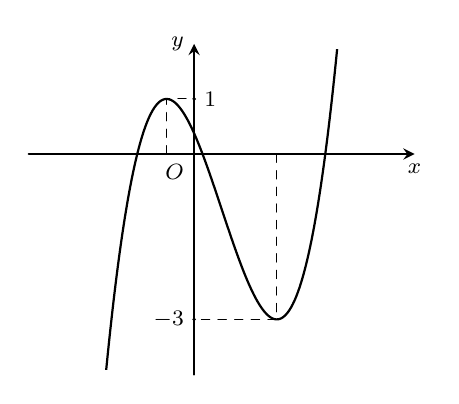
\begin{tikzpicture}[scale=.7,>=stealth, font=\footnotesize, line join=round, line cap=round,thick]
			\def\a{1} \def\b{-3} \def\c{0} \def\d{1} % Hệ số
			\def\xmin{-3} \def\xmax{4}
			\def\ymin{-4} \def\ymax{2}
			%\draw[color=gray!50,dashed] (\xmin,\ymin) grid (\xmax,\ymax);
			\draw[->] (\xmin,0)--(\xmax,0) node [below]{$x$};
			\draw[->] (0,\ymin)--(0,\ymax) node [left]{$y$};
			\node at (0,0) [below left]{$O$};
			\clip (\xmin+0.1,\ymin+0.1) rectangle (\xmax-0.1,\ymax-0.1);
			\draw[dashed,thin] (-.5,0)--(-.5,1)--(0,1)
			(1.5,0)--(1.5,-3)--(0,-3) ;
			\path[fill=black] (0,1) circle (1pt) node[right]{$1$} (0,-3) circle (1pt) node[left]{$-3$};
			\draw[smooth,samples=300]plot(\x,{\a*(\x+.5)^3+\b*(\x+.5)^2+\c*(\x+.5)+\d});
		\end{tikzpicture}
	\end{center}
	Tất cả các giá trị của tham số $m$ để hàm số $y=\left|f(x)+m\right|$ có ba điểm cực trị là:
	\choice
	{\True $m\le-1$ hoặc $m\ge 3$}
	{$m\le-3$ hoặc $m\ge 1$}
	{$m=-1$ hoặc $m=3$}
	{$1\le m\le 3$}
	\loigiai{
		\textbf{Cách 1:}\\
		Do $y=f(x)+m$ là hàm số bậc ba.\\
		Khi đó, hàm số $y=\left|f(x)+m\right|$ có ba điểm cực trị.\\
		$\Leftrightarrow$ hàm số $y=f(x)+m$ có $y_{\text{CĐ}}.y_{\text{CT}}\ge 0$.\\
		(hình minh họa).
		\begin{center}
			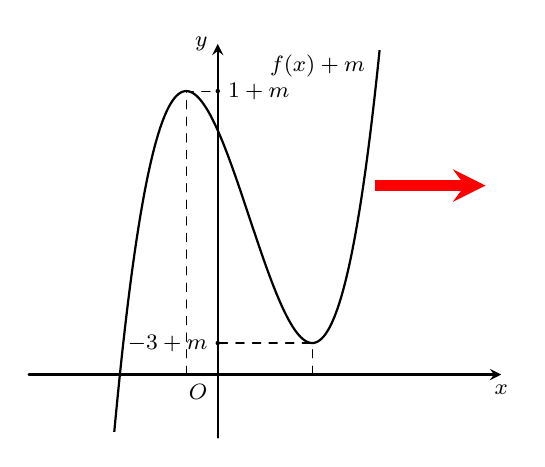
\begin{tikzpicture}[scale=.8,>=stealth, font=\footnotesize, line join=round, line cap=round,thick]
				\def\a{1} \def\b{-3} \def\c{0} \def\d{4.5} % Hệ số
				\def\xmin{-3} \def\xmax{4.5}
				\def\ymin{-1} \def\ymax{5.25}
				%\draw[color=gray!50,dashed] (\xmin,\ymin) grid (\xmax,\ymax);
				\draw[->] (\xmin,0)--(\xmax,0) node [below]{$x$};
				\draw[->] (0,\ymin)--(0,\ymax) node [left]{$y$};
				\node at (0,0) [below left]{$O$};
				\clip (\xmin+0.1,\ymin+0.1) rectangle (\xmax-0.1,\ymax-0.1);
				\draw[dashed,thin] (-.5,0)--(-.5,4.5)--(0,4.5)
				(1.5,0)--(1.5,.5)--(0,.5) ;
				\path[fill=black] (0,4.5) circle (1pt) node[right]{$1+m$} (0,.5) circle (1pt) node[left]{$-3+m$};
				\draw[smooth,samples=300] plot(\x,{\a*(\x+.5)^3+\b*(\x+.5)^2+\c*(\x+.5)+\d});
				\path (2.5,4.9) node[left]{$f(x)+m$};
				\draw[red,line width=4pt,line cap=butt,->] (2.5,3)--(4.25,3);
			\end{tikzpicture}
			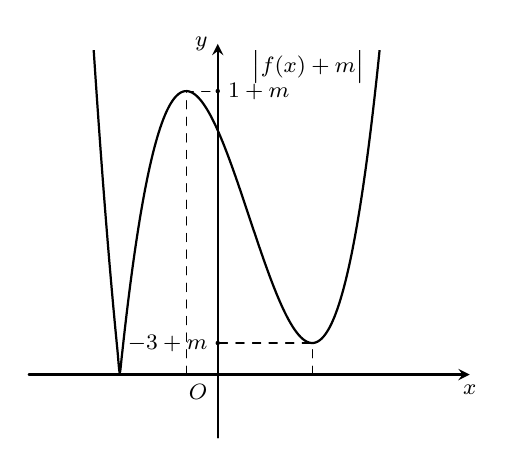
\begin{tikzpicture}[scale=.8,>=stealth, font=\footnotesize, line join=round, line cap=round,thick]
				\def\a{1} \def\b{-3} \def\c{0} \def\d{4.5} % Hệ số
				\def\xmin{-3} \def\xmax{4}
				\def\ymin{-1} \def\ymax{5.25}
				%\draw[color=gray!50,dashed] (\xmin,\ymin) grid (\xmax,\ymax);
				\draw[->] (\xmin,0)--(\xmax,0) node [below]{$x$};
				\draw[->] (0,\ymin)--(0,\ymax) node [left]{$y$};
				\node at (0,0) [below left]{$O$};
				\clip (\xmin+0.1,\ymin+0.1) rectangle (\xmax-0.1,\ymax-0.1);
				\draw[dashed,thin] (-.5,0)--(-.5,4.5)--(0,4.5)
				(1.5,0)--(1.5,.5)--(0,.5) ;
				\path[fill=black] (0,4.5) circle (1pt) node[right]{$1+m$} (0,.5) circle (1pt) node[left]{$-3+m$};
				\draw[smooth,samples=300] plot(\x,{abs(\a*(\x+.5)^3+\b*(\x+.5)^2+\c*(\x+.5)+\d)});
				\path (2.5,4.9) node[left]{$\big|f(x)+m\big|$};
			\end{tikzpicture}
		\end{center}
		$\Leftrightarrow\left(1+m\right)\left(-3+m\right)\ge 0\Leftrightarrow\left[\begin{aligned}
			&m\le-1\\
			&m\ge 3\\
		\end{aligned}\right.$.\\
		\textbf{Cách 2:}\\
		Ta có $y=\left|f(x)+m\right|$=$\sqrt{\left(f(x)+m\right)^2}\Rightarrow{y}'=\dfrac{\left(f(x)+m\right).f'(x)}{\sqrt{\left(f(x)+m\right)^2}}$.\\
		Để tìm cực trị của hàm số $y=\left| f(x)+m\right|$, ta tìm $x$ thỏa mãn $y'=0$ hoặc $y'$ không xác định.\\
		$\Leftrightarrow\left[\begin{aligned}
			&{f}'(x)=0(1)\\
			&f(x)=-m(2)\\
		\end{aligned}\right.$.\\
		Dựa vào đồ thị, suy ra hàm số có $2$ điểm cực trị $x_1$, $x_2$ trái dấu.\\
		Suy ra $(1)$ có hai nghiệm $x_1$, $x_2$ trái dấu.\\
		Vậy để đồ thị hàm số có $3$ cực trị thì $(2)$ có một nghiệm khác $x_1$, $x_2$.\\
		Số nghiệm của $(2)$ chính là số giao điểm của đồ thị $(C)$ và đường thẳng $y=-m$.\\
		Do đó để $(2)$ có một nghiệm thì dựa vào đồ thị ta có điều kiện: $\left[\begin{aligned}
			&-m\ge 1\\
			&-m\le-3\\
		\end{aligned}\right.\Leftrightarrow\left[\begin{aligned}
			&m\le-1\\
			&m\ge 3\\
		\end{aligned}\right.$.\\
		\textbf{Chú ý:}\\
		Nếu $x=x_0$ là cực trị của hàm số $y=f(x)$ thì $f'\left(x_0\right)=0$ hoặc không tồn tại $f'\left(x_0\right)$.
	}
\end{ex}
\begin{ex}[Đề Tham Khảo 2018]%Câu 2%[2D1G2-2]
	Có bao nhiêu giá trị nguyên của tham số $m$ để hàm số $y=\left|3x^4-4x^3-12x^2+m\right|$ có $7$ điểm cực trị?
	\choice
	{$5$}
	{$6$}
	{\True $4$}
	{$3$}
	\loigiai{
		$y=\left|f(x)\right|=\left|3x^4-4x^3-12x^2+m\right|$\\
		Ta có: $f'(x)=12x^3-12x^2-24x$; $f'(x)=0\Leftrightarrow x=0$ hoặc $x=-1$ hoặc $x=2$.\\
		\begin{center}
			
\begin{tikzpicture}[thick,>=stealth,line cap=round,line join=round,font=\footnotesize]
				\tkzTabInit[nocadre,lgt=1.25,espcl=2.5]
				{$x$/0.8,$f'(x)$/0.8,$f(x)$/2.5}
				{$-\infty$,$-1$,$0$,$2$,$+\infty$}
				\tkzTabLine{,-,0,+,0,-,0,+}
				\tkzTabVar{+/$+\infty$,-/$m-5$,+/$m$,-/$m-32$,+/$+\infty$}
			\end{tikzpicture}
		\end{center}
		Do hàm số $f(x)$ có ba điểm cực trị nên hàm số $y=\left|f(x)\right|$ có $7$ điểm cực trị khi\\
		Phương trình $f(x)=0$ có $4$ nghiệm $\Leftrightarrow\left\{\begin{aligned}
			&m>0\\
			&m-5<0\\
		\end{aligned}\right.\Leftrightarrow 0<m<5$.\\
		Vậy có $4$ giá trị nguyên thỏa đề bài là $m=1$; $m=2$; $m=3$; $m=4$.
	}
\end{ex}
\begin{ex}[Gia Bình 2019]%Câu 3%[2D1G2-2]
	Cho hàm số $y=f(x)$ có bảng biến thiên như sau.
	\begin{center}
		
\begin{tikzpicture}[line cap=round,line join=round,font=\footnotesize,thick]
			\tkzTabInit[nocadre=true,lgt=1.2,espcl=2.5,deltacl=0.6]
			{$x$ /0.6, $y'$ /0.6, $y$ /2.5}
			{$-\infty$,$-2$,$4$,$+\infty$}
			\tkzTabLine{,+,$0$,-,$0$,+,}
			\tkzTabVar{-/$-\infty$,+/$6$,-/$2$,+/$+\infty$}
		\end{tikzpicture}
	\end{center}
	Hàm số $y=f\left(\left|x-3\right|\right)$ có bao nhiêu điểm cực trị
	\choice
	{$5$}
	{$6$}
	{\True $3$}
	{$1$}
	\loigiai{
	$y=f\left(\left|x-3\right|\right)(1)$, Đặt $t=|x-3|$, $t\ge 0$ Thì $(1)$ trở thành:$y=f(t)$ $(t\geq 0)$.\\
	Có $t=\sqrt{(x-3)^2}\Rightarrow t'=\dfrac{x-3}{\sqrt{(x-3)^2}}$.\\
	Có $y_x'=t_x'f'(t)$.\\
	$y_x'=0\Leftrightarrow t_x'f'(t)=0\Leftrightarrow\left[\begin{aligned}
			&t_x'=0\\
			&f'(t)=0\\
		\end{aligned}\right.\Leftrightarrow\left[\begin{aligned}
			&x=3\\
			&t=-2~(\mathrm{L})\\
			&t=4\\
		\end{aligned}\right.\Leftrightarrow\left[\begin{aligned}
			&x=3\\
			&x=7\\
			&x=-1\\
		\end{aligned}\right.$.\\
		Lấy $x=8$ có $t'(8)f'(5)>0$, đạo hàm đổi dấu qua các nghiệm đơn nên ta có bảng biến thiên:
	\begin{center}
		\begin{tikzpicture}[font=\footnotesize,thick]
			\tkzTabInit[nocadre,lgt=1,espcl=2.5]
				{$x$/0.8,$y'$/0.8,$y$/2.5}
				{$-\infty$,$-1$,$3$,$7$,$+\infty$}
				\tkzTabLine{,-,z,+,d,-,z,+}
				\tkzTabVar{+/$+\infty$,-/$\text{CT}$,+/$\text{CĐ}$,-/$\text{CT}$,+/$+\infty$}
		\end{tikzpicture}
	\end{center}
	Dựa vào bảng biến thiên thì hàm số $y=f\left(\left|x-3\right|\right)$ có $3$ cực trị.
	}
\end{ex}
\begin{ex}[Cụm Liên Trường Hải Phòng 2019]%Câu 4%[2D1G2-1]
	Tìm số các giá trị nguyên của tham số $m$ để đồ thị hàm số $y=\left|x^4-2m{x^2}+2m^2+m-12\right|$ có bảy điểm cực trị
	\choice
	{$1$}
	{$4$}
	{\True $0$}
	{$2$}
	\loigiai{
	Đồ thị hàm số $y=\left|x^4-2m{x^2}+2m^2+m-12\right|$ có bảy điểm cực trị khi và chỉ khi đồ thị hàm số $y=x^4-2m{x^2}+2m^2+m-12$ cắt trục hoành tại bốn điểm phân biệt.\\
		$x^4-2m{x^2}+2m^2+m-12=0$ có bốn nghiệm phân biệt khi và chỉ khi $\left\{\begin{aligned}
			&{m^2}-\left(2m^2+m-12\right)>0\\
			&2m>0\\
			&2m^2+m-12>0\\
		\end{aligned}\right.\Leftrightarrow\left\{\begin{aligned}
			&-4<m<3\\
			&m>0\\
			&m<\dfrac{-1-\sqrt{97}}{4}\vee m>\dfrac{-1+\sqrt{97}}{4}\\
		\end{aligned}\right.$ $\Leftrightarrow\dfrac{-1+\sqrt{97}}{4}<m<3$.\\
	Vậy không có giá trị nguyên của tham số $m$ để đồ thị hàm số $y=\left|x^4-2m{x^2}+2m^2+m-12\right|$ có bảy điểm cực trị.
	}
\end{ex}
\begin{ex}[Sở Vĩnh Phúc 2019]%Câu 5%[2D1G2-2]
	Có bao nhiêu giá trị nguyên của tham số $m$ để hàm số $y=\left|3x^4-4x^3-12x^2+m^2\right|$ có đúng 5 điểm cực trị?
	\choice
	{$5$}
	{$7$}
	{\True $6$}
	{$4$}
	\loigiai{
	Xét hàm số $f(x)=3x^4-4x^3-12x^2+m^2$; $f'(x)=12x^3-12x^2-24x$.\\
	$f'(x)=0\Leftrightarrow{x_1}=0;{x_2}=-1;{x_3}=2$. Suy ra, hàm số $y=f(x)$ có $3$ điểm cực trị.\\
	$\Rightarrow $ Hàm số $y=\left|3x^4-4x^3-12x^2+m^2\right|$ có $5$ điểm cực trị khi đồ thị hàm số $y=f(x)$ cắt trục hoành tại $2$ điểm phân biệt $\Leftrightarrow $ $3x^4-4x^3-12x^2+m^2=0$ có $2$ nghiệm phân biệt.\\
	Phương trình $3x^4-4x^3-12x^2+m^2=0\Leftrightarrow-3x^4+4x^3+12x^2=m^2$ $(1)$.\\
	Xét hàm số $g(x)=-3x^4+4x^3+12x^2$; $g'(x)=-12x^3+12x^2+24x$.\\
	Bảng biến thiên:
	\begin{center}
		
\begin{tikzpicture}[font=\footnotesize,thick]
			\tkzTabInit[nocadre,lgt=1,espcl=2.5]
			{$x$/0.8,$g'(x)$/0.8,$g(x)$/2.5}
			{$-\infty$,$-1$,$0$,$2$,$+\infty$}
			\tkzTabLine{,+,0,-,0,+,0,-}
			\tkzTabVar{-/$-\infty$,+/$5$,-/$0$,+/$32$,-/$-\infty$}
		\end{tikzpicture}
	\end{center}
	Phương trình $(1)$ có $2$ nghiệm phân biệt $\Leftrightarrow\left[\begin{aligned}
			&{m^2}<0\\
			& 5<m^2<32\\
		\end{aligned}\right.\Leftrightarrow\sqrt{5}<\left|m\right|<\sqrt{32}$.\\
		Vậy $m\in\left\{3;4;5;-3;-4;-5\right\}$.
	}
\end{ex}
\begin{ex}[Chuyên Vĩnh Phúc 2019]%Câu 6%[2D1G2-2]
	Có bao nhiêu giá trị nguyên dương của tham số $m$ để hàm số $y=\left|3x^4-4x^3-12x^2+m\right|$ có $5$ điểm cực trị?
	\choice
	{$16$}
	{$44$}
	{\True $26$}
	{$27$}
	\loigiai{
		Đặt: $g(x)=3x^4-4x^3-12x^2+m$.\\
		Ta có: $g'(x)=12x^3-12x^2-24x=0\Leftrightarrow\left[\begin{aligned}
			&x=2\Rightarrow y=m-32\\
			&x=-1\Rightarrow y=m-5\\
			&x=0\Rightarrow y=m\\
		\end{aligned}\right.$.
		\begin{center}
			
\begin{tikzpicture}[font=\footnotesize,thick]
				\tkzTabInit[nocadre,lgt=1.2,espcl=2.5]
				{$x$/0.8,$g'(x)$/0.8,$g(x)$/2.5}
				{$-\infty$,$-1$,$0$,$1$,$+\infty$}
				\tkzTabLine{,-,0,+,0,-,0,+}
				\tkzTabVar{+/$+\infty$,-/$m-5$,+/$m$,-/$m-32$,+/$+\infty$}
			\end{tikzpicture}
		\end{center}
		Dựa vào bảng biến thiên, hàm số có $y=\left|g(x)\right|$ có $5$ điểm cực trị\\ khi $\left[\begin{aligned}
			&m<0\\
			&\left\{\begin{aligned}
				&m-5>0\\
				&m-32<0\\
			\end{aligned}\right.\\
		\end{aligned}\right.\Leftrightarrow\left[\begin{aligned}
			& m<0\\
			& 5<m<32\\
		\end{aligned}\right.$.\\
		Vì $m$ là số nguyên dương cho nên có $26$ số $m$ thỏa đề bài.
	}
\end{ex}
\begin{ex}[THPT Lương Thế Vinh Hà Nội 2019]%Câu 7%[2D1G2-1]
	Cho hàm số $y=\left|x^4-2mx^2+2m-1\right|$ với $m$ là tham số thực. Số giá trị nguyên trong khoảng $\left[-2;2\right]$ của $m$ để hàm số đã cho có $3$ điểm cực trị là
	\choice
	{$2$}
	{\True $4$}
	{$3$}
	{$1$}
	\loigiai{
		Đặt $f(x)=x^4-2m{x^2}+2m-1$, $f'(x)=4x^3-4mx$, $f'(x)=0\Leftrightarrow\left[\begin{aligned}
			&x=0\\
			&{x^2}=m\\
		\end{aligned}\right.$.\\
		\textbf{Trường hợp 1:} hàm số có một cực trị $\Rightarrow m\in\left[-2;0\right]$.\\
		Đồ thị hàm số $y=f(x)$ có một điểm cực trị là $A\left(0;2m-1\right)$.\\
		Do $m\in\left[-2;0\right]$ $\Rightarrow y_A=2m-1<0$ nên đồ thị hàm số $y=f(x)$ cắt trục hoành tại $2$ điểm phân biệt nên hàm số $y=\left| f(x)\right|$ có $3$ cực trị $\Rightarrow$ có $3$ giá trị nguyên của $m$ thỏa yêu cầu bài toán.\\
		\textbf{Trường hợp 2:} hàm số có ba cực trị $\Rightarrow m\in\left(0;2\right]$.\\
		Khi đó đồ thị hàm số có $3$ điểm cực trị là $A\left(0;2m-1\right)$, $B\left(\sqrt{m};-m^2+2m-1\right)$, $C\left(-\sqrt{m};-m^2+2m-1\right)$.\\
		Do $a=1>0$ nên hàm số $y=\left|f(x)\right|$ có $3$ điểm cực trị khi hàm số $y=f(x)$ có $y_B=y_C\ge 0$\\
		$\Leftrightarrow-m^2+2m-1\ge 0\Leftrightarrow m=1$.\\
		Nếu $y_B=y_C<0$ (trong bài toán này không xảy ra) thì hàm số có ít nhất $5$ điểm cực trị.\\
		Vậy có $4$ giá trị của $m$ thỏa yêu cầu bài toán.
	}
\end{ex}
\begin{ex}[Chuyên Bắc Ninh 2019]%Câu 8%[2D1G2-2]
	Tập hợp các giá trị của $m$ để hàm số $y=\left|3x^4-4x^3-12x^2+m-1\right|$ có $7$ điểm cực trị là:
	\choice
	{$(0;6)$}
	{$(6;33)$}
	{$(1;33)$}
	{\True $(1;6)$}
	\loigiai{
		Xét hàm số $f(x)=3x^4-4x^3-12x^2+m-1$.\\
		Có $\lim\limits_{x\to+\infty}f(x)=+\infty$, $\lim\limits_{x\to-\infty}f(x)=-\infty$.\\
		$f'(x)=12x^3-12x^2-24 x=12 x\left(x^2-x-2\right)$\\
		$f'(x)=0\Leftrightarrow\left[\begin{aligned}
			&x=0\\
			&x=-1\\
			&x=2\\
		\end{aligned}\right.$.\\
		Bảng biến thiên:
		\begin{center}
			
\begin{tikzpicture}[font=\footnotesize,thick,>=stealth]
				\tkzTabInit[nocadre,lgt=1.25,espcl=2.5]
				{$x$/0.8,$f'(x)$/0.8,$f(x)$/2.5}
				{$-\infty$,$-1$,$0$,$2$,$+\infty$}
				\tkzTabLine{,-,0,+,0,-,0,+}
				\tkzTabVar{+/$+\infty$,-/$m-6$,+/$m-1$,-/$m-33$,+/$+\infty$}
			\end{tikzpicture}
		\end{center}
		Từ bảng biến thiên, ta có hàm số $y=\left|f(x)\right|$ có $7$ điểm cực trị $\Leftrightarrow$ đồ thị hàm số $y=f(x)$ cắt $Ox$ tại $4$ điểm phân biệt $\Leftrightarrow m-6<0<m-1\Leftrightarrow 1<m<6$.
	}
\end{ex}
\begin{ex}[THPT Kinh Môn-2018]%Câu 9%[2D1G2-1]
	Cho hàm số $y=f(x)=x^3-(2m-1){x^2}+(2-m)x+2$. Tìm tất cả các giá trị của tham số $m$ để hàm số $y=f(\left|x\right|)$ có $5$ điểm cực trị.
	\choice
	{$\dfrac{5}{4}<m\le 2$}
	{$-2<m<\dfrac{5}{4}$}
	{$-\dfrac{5}{4}<m<2$}
	{\True $\dfrac{5}{4}<m<2$}
	\loigiai{
		Ta có: $y'=3x^2-2\left(2m-1\right)x+2-m$.\\
		Hàm số $y=f(\left| x\right|)$ có $5$ điểm cực trị khi và chỉ khi hàm số $f(x)$ có hai cực trị dương.\\
		$\Leftrightarrow\left\{\begin{aligned}
			&\Delta >0\\
			&S>0\\
			&P>0\\
		\end{aligned}\right.\Leftrightarrow\left\{\begin{aligned}
			&{\left(2m-1\right)^2}-3\left(2-m\right)>0\\
			&\dfrac{2\left(2m-1\right)}{3}>0\\
			&\dfrac{2-m}{3}>0\\
		\end{aligned}\right.\Leftrightarrow\left\{\begin{aligned}
			&4m^2-m-5>0\\
			&m>\dfrac{1}{2}\\
			&m<2\\
		\end{aligned}\right.\Leftrightarrow\dfrac{5}{4}<m<2$.
	}
\end{ex}
\begin{ex}[Chuyên Đh Vinh-2018]%Câu 10%[2D1G2-1]
	Cho hàm số $y=f(x)$ có đạo hàm $f'(x)=\left(x^3-2x^2\right)\left(x^3-2x\right)$ với mọi $x\in\mathbb{R}$. Hàm số $\left|f\left(1-2018x\right)\right|$ có nhiều nhất bao nhiêu điểm cực trị?
	\choice
	{\True $9$}
	{$2018$}
	{$2022$}
	{$11$}
	\loigiai{
		Ta có $f'(x)=x^3\left(x-2\right)\left(x^2-2\right)=0$ có $4$ nghiệm và đổi dấu $4$ lần nên hàm số $y=f(x)$ có $4$ cực trị. Suy ra $f(x)=0$ có tối đa $5$ nghiệm phân biệt.\\
		Do đó $y=\left|f\left(1-2018x\right)\right|$ có tối đa $9$ cực trị.
	}
\end{ex}
\begin{ex}[THPT Thạch Thanh 2-Thanh Hóa-2018]%Câu 11%[2D1G2-2]
	Hình vẽ bên là đồ thị của hàm số $y=f(x)$.
	\begin{center}
		%\begin{tikzpicture}[line join=round, line cap=round, >=stealth, scale=.7, thick,font=\footnotesize]
		%\draw[->] (-4.5,0)--(4.5,0)node[below]{$x$};
		%\draw[->] (0,-7)--(0,4)node[left]{$y$};
		%\draw [line width=1pt,blue]
		%(-4,4) .. controls + (-85:0.75) and + (-180:0.75) ..
		%(-3,-3) .. controls + (0:0.75) and + (-180:0.75) ..
		%(-.8,2) .. controls + (0:0.75) and + (-180:0.75) ..
		%(2,-6) .. controls + (0:0.75) and + (-180:0.05) ..
		%(4,4) ;
		%\draw[dashed] (0,2)--(-.8,2)--(-.8,0) (0,-3)--(-3,-3)--(-3,0) (0,-6)--(2,-6)--(2,0)
		%;
		%\path
		%(0,-6) node[left]{$-6$}
		%(0,-3) node[right]{$-3$}
		%(0,2) node[right]{$2$}
		%(0,0) node[below left]{$O$} ;
		%\foreach \diemx/\diemy in {0/0, 0/-6,0/-3,0/2}
		%\fill (\diemx,\diemy)circle(1.2pt);
%	\end{tikzpicture}
	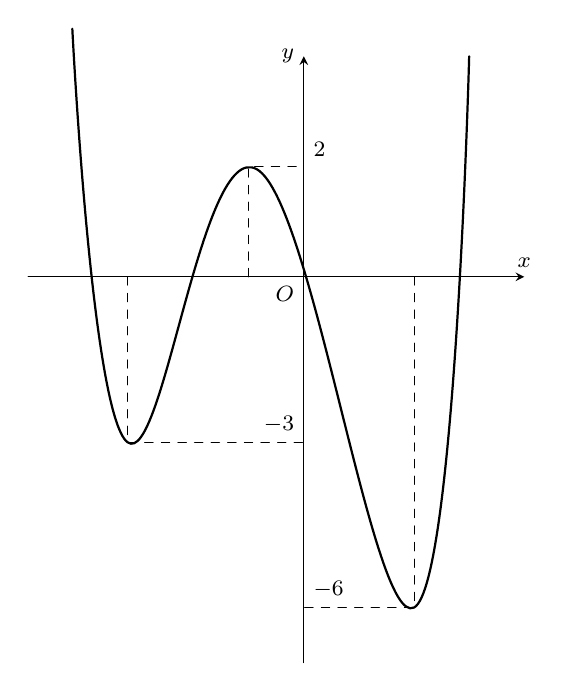
\begin{tikzpicture}[line join = round, line cap = round, >=stealth, font=\footnotesize, scale=0.7]
		%\tikzset{label style/.style={font=\footnotesize}}
		\draw[->] (-5,0)--(0,0) node[below left]{$O$} -- (4,0) node[above]{$x$};
		\draw[->] (0,-7) -- (0,4) node[left]{$y$};
		\draw[dashed] (-3.2,0)-- (-3.2,-3)--(0,-3)node[above left]{$-3$} (-1,0)--(-1,2)--(0,2)node[above right]{$2$} (2,0)--(2,-6)--(0,-6)node[above right]{$-6$};
		\draw[thick] plot[smooth,tension=0.7] coordinates{(-4.2,4.5) (-3.2,-3) (-0.85,1.95) (2,-6) (3,4)};
	\end{tikzpicture}
\end{center}
Gọi $S$ là tập hợp các giá trị nguyên dương của tham số $m$ để hàm số $y=\left|f\left(x-1\right)+m\right|$ có $5$ điểm cực trị. Tổng giá trị tất cả các phần tử của $S$ bằng
	\choice
	{$9$}
	{\True $12$}
	{$18$}
	{$15$}
	\loigiai{
	Nhận xét: Số giao điểm của $(C)\colon y=f(x)$ với $Ox$ bằng số giao điểm của $\left(C'\right):y=f\left(x-1\right)$ với $Ox$.\\
	Vì $m>0$ nên $\left(C''\right):y=f\left(x-1\right)+m$ có được bằng cách tịnh tiến $\left(C'\right):y=f\left(x-1\right)$ lên trên $m$ đơn vị.
	\begin{center}
		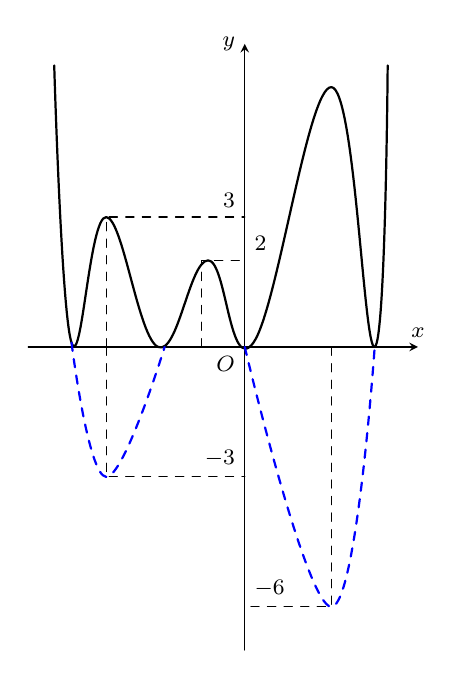
\begin{tikzpicture}[line join = round, line cap = round, >=stealth, font=\footnotesize, scale=0.55]
			%\tikzset{label style/.style={font=\footnotesize}}
			\draw[->] (-5,0)--(0,0) node[below left]{$O$} -- (4,0) node[above]{$x$};
			\draw[->] (0,-7) -- (0,7) node[left]{$y$};
			\draw[dashed] (-3.2,0)-- (-3.2,3)--(0,3)node[above left]{$3$}
			(-3.2,0)-- (-3.2,-3)--(0,-3)node[above left]{$-3$}
			(-1,0)--(-1,2)--(0,2)node[above right]{$2$}
			(2,0)--(2,-6)--(0,-6)node[above right]{$-6$};
			\draw[thick] plot[smooth,tension=0.7] coordinates{(-4.4,6.5) (-4,.1) (-3.2,3) (-2,0) (-0.85,2) (.2,.1) (2,6) (3,0) (3.3,6.5)};
			\draw[dashed,thick,blue] plot[smooth,tension=0.7] coordinates{ (-4,.1) (-3.2,-3) (-1.85,0)};
			\draw[dashed,thick,blue] plot[smooth,tension=0.7] coordinates{ (0,0) (2,-6) (3,0)};
		\end{tikzpicture}
		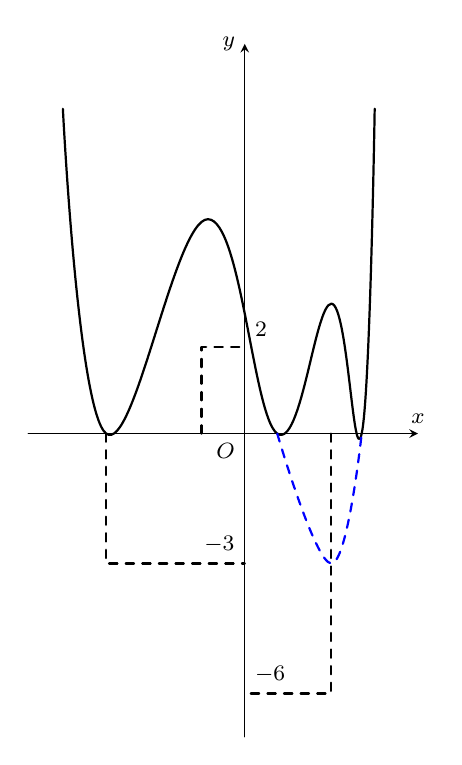
\begin{tikzpicture}[line join = round, line cap = round, >=stealth, font=\footnotesize, scale=0.55]
			%\tikzset{label style/.style={font=\footnotesize}}
			\draw[->] (-5,0)--(0,0) node[below left]{$O$} -- (4,0) node[above]{$x$};
			\draw[->] (0,-7) -- (0,9) node[left]{$y$};
			\draw[dashed,thick] (-3.2,0)-- (-3.2,-3)--(0,-3)node[above left]{$-3$} (-1,0)--(-1,2)--(0,2)node[above right]{$2$} (2,0)--(2,-6)--(0,-6)node[above right]{$-6$};
			\draw[thick] plot[smooth,tension=0.7] coordinates{(-4.2,7.5) (-3.2,0) (-0.85,4.95) (.75,0) (2,3) (2.7,0) (3,7.5)};
			\draw[dashed,thick,blue] plot[smooth,tension=0.7] coordinates{(.75,0) (2,-3) (2.7,0)};
		\end{tikzpicture}
		\begin{tikzpicture}[line join = round, line cap = round, >=stealth, font=\footnotesize, scale=0.55]
			%\tikzset{label style/.style={font=\footnotesize}}
			\draw[->] (-5,0)--(0,0) node[below left]{$O$} -- (4,0) node[above]{$x$};
			\draw[->] (0,-7) -- (0,11) node[left]{$y$};
			\draw[dashed] (-3.2,0)-- (-3.2,-3)--(0,-3)node[above left]{$-3$} (-1,0)--(-1,2)--(0,2)node[above right]{$2$} (2,0)--(2,-6)--(0,-6)node[above right]{$-6$};
			\draw[thick] plot[smooth,tension=0.7] coordinates{(-4.2,10.5) (-3.2,3) (-0.85,7.95) (2,0) (3,10.5)};
		\end{tikzpicture}
	\end{center}
	\textbf{Trường hợp 1:} $0<m<3$. Đồ thị hàm số có $7$ điểm cực trị. Loại.\\
	\textbf{Trường hợp 2:} $m=3$. Đồ thị hàm số có $5$ điểm cực trị. Nhận.\\
	\textbf{Trường hợp 3:} $3<m<6$. Đồ thị hàm số có $5$ điểm cực trị. Nhận.\\
	\textbf{Trường hợp 4:} $m\ge 6$. Đồ thị hàm số có $3$ điểm cực trị. Loại.\\
	Vậy $3\le m<6$. Do $m\in{\mathbb{Z}^*}$ nên $m\in\left\{ 3;4;5\right\}$.\\
	Vậy tổng giá trị tất cả các phần tử của $S$ bằng $12$.
}
\end{ex}
\begin{ex}[THPT Quảng Yên-Quảng Ninh-2018]%Câu 12%[2D1G2-2]
	Có bao nhiêu giá trị nguyên của tham số $m$ để hàm số $y=\left|3x^4+4x^3-12x^2+\dfrac{m}{2}\right|$ có $7$ điểm cực trị?
	\choice
	{$3$}
	{\True $9$}
	{$6$}
	{$4$}
	\loigiai{
	Ta có $y=\left|3x^4+4x^3-12x^2+\dfrac{m}{2}\right|=\sqrt{\left(3x^4+4x^3-12x^2+\dfrac{m}{2}\right)^2}$.\\
	$\Rightarrow{y}'=\dfrac{\left(12x^3+12x^2-24x\right)\left(3x^4+4x^3-12x^2+\dfrac{m}{2}\right)}{\sqrt{\left(3x^4+4x^3-12x^2+\dfrac{m}{2}\right)^2}}$.\\
	$\Rightarrow{y}'=0\Leftrightarrow\left[\begin{aligned}
		&12x^3+12x^2-24x=0~(1)\\
		&3x^4+4x^3-12x^2+\dfrac{m}{2}=0~(2)\\
	\end{aligned}\right.$.\\
	Từ $(1)\Rightarrow\left[\begin{aligned}
		&x=0\\
		&x=1\\
		&x=-2\\
	\end{aligned}\right.$.\\
	Vậy để hàm số có $7$ điểm cực trị thì $(2)$ phải có bốn nghiệm phân biệt khác $\left\{ 0;1;-2\right\}$.\\
	Xét hàm số $f(x)=3x^4+4x^3-12x^2+\dfrac{m}{2}\Rightarrow f'(x)=12x^3+12x^2-24x\Rightarrow f'(x)=0\Leftrightarrow\left[\begin{aligned}
		&x=0\\
		&x=1\\
		&x=-2\\
	\end{aligned}\right.$.
	\begin{center}
		
\begin{tikzpicture}[line cap=round, line join=round, line width=1pt, scale=1, font=\footnotesize]
			\tkzTabInit[nocadre,lgt=1.2,espcl=2.5]
			{$x$/0.8,$f'(x)$/0.8,$f(x)$/2.5}
			{$-\infty$,$-2$,$0$,$1$,$+\infty$}
			\tkzTabLine{,-,0,+,0,-,0,+}
			\tkzTabVar{+/$+\infty$,-/$-32+\dfrac{m}{2}$,+/$\dfrac{m}{2}$,-/$-5+\dfrac{m}{2}$,+/$+\infty$}
		\end{tikzpicture}
	\end{center}
	Để $(2)$ có $4$ nghiệm phân biệt thì $f(x)$ cắt trục hoành tại $4$ điểm phân biệt $\Rightarrow\left\{\begin{aligned}
		&-5+\dfrac{m}{2}<0\\
		&\dfrac{m}{2}>0\\
	\end{aligned}\right.\Leftrightarrow\left\{\begin{aligned}
		&m<10\\
		&m>0\\
	\end{aligned}\right.\Leftrightarrow 0<m<10$.\\
	Vậy có $9$ giá trị nguyên của tham số $m$ để hàm số $y=\left|3x^4+4x^3-12x^2+\dfrac{m}{2}\right|$ có $7$ điểm cực trị.
	}
\end{ex}
\begin{ex}[THPT Nguyễn Tất Thành-Yên Bái-2018]%Câu 13%[2D1G2-2]
	Có bao nhiêu giá trị nguyên của tham số $m$ để hàm số $y=\left|x^3-3x^2+m\right|$ có $5$ điểm cực trị?
	\choice
	{$5$}
	{\True $3$}
	{$6$}
	{$4$}
	\loigiai{
	Hàm số $y=\left|x^3-3x^2+m\right|$ có $5$ điểm cực trị $\Leftrightarrow $ đồ thị hàm số $y=x^3-3x^2+m$ có hai điểm cực trị và nằm về hai phía của trục hoành $\Leftrightarrow$ phương trình $x^3-3x^2+m=0~(1)$ có ba nghiệm phân biệt.\\
	Xét bbt của hàm số $y=x^3-3x^2$\\
	$y'=3x^2-6x=0\Rightarrow\left[\begin{aligned}
		&x=0\\
		&x=2\\
	\end{aligned}\right.$.
	\begin{center}
		
\begin{tikzpicture}[thick,font=\footnotesize,>=stealth]
			\tkzTabInit[nocadre,lgt=1.25,espcl=2.5]
			{$x$/0.8,$y'$/0.8,$y$/2.5}
			{$-\infty$,$0$,$2$,$+\infty$}
			\tkzTabLine{,+,0,-,0,+}
			\tkzTabVar{-/$-\infty$,+/$0$,-/$-4$,+/$+\infty$}
		\end{tikzpicture}
	\end{center}
	Từ đó ta được $(1)$ có ba nghiệm phân biệt $\Leftrightarrow-4<-m<0\Leftrightarrow 0<m<4$. Vậy có $3$ giá trị nguyên của $m$ thỏa mãn.
}
\end{ex}
\begin{ex}[Chuyên Nguyễn Thị Minh Khai-Sóc Trăng-2018]%Câu 14%[2D1G2-2]
Có bao nhiêu giá trị nguyên của tham số $m$ để hàm số $y=\left|3x^5-25x^3+60x+m\right|$ có 7 điểm cực trị?
	\choice
	{\True $42$}
	{$21$}
	{$40$}
	{$20$}
	\loigiai{
	$\begin{aligned}
		&y=3x^5-25x^3+60x+m\\
		&\Rightarrow{y}'=15x^4-75x^2+60\\
		&{y}'=0\Leftrightarrow\left[\begin{aligned}
			&{x^2}=1\\
			&{x^2}=4\\
		\end{aligned}\right.\Leftrightarrow\left[\begin{aligned}
			&x=-2\Rightarrow y=m-16\\
			&x=-1\Rightarrow y=m-38\\
			&x=1\Rightarrow y=m+38\\
			&x=2\Rightarrow y=m+16\\
		\end{aligned}\right.\\
	\end{aligned}$.
	\begin{center}
		\begin{tikzpicture}[line cap=round, line join=round, font=\footnotesize, scale=1, >=stealth, thick]
			\tkzTabInit[nocadre,lgt=1,espcl=2.5]
			{$x$/0.8,$y'$/0.8,$y$/3.2}
			{$-\infty$,$-2$,$-1$,$1$,$2$,$+\infty$}
			\tkzTabLine{,+,0,-,0,+,0,-,0,+}
			\tkzTabVar{%-/$-\infty$,+/$m-16$,-/$m-38$,+/$m+38$,-/$m+16$,+/$+\infty$
			}
			\path (N13) node[above](A){$-\infty$}
			($(N23)!.45!(N22)$) node[above](B){$m-16$}
			(N33) node[above](C){$m-38$}
			(N42) node[below](D){$m+38$}
			($(N53)!.55!(N52)$) node[below](E){$m+16$}
			(N62) node[below](F){$+\infty$}
			;
			\draw[->] (A)--(B);
			\draw[->] (B)--(C);
			\draw[->] (C)--(D);
			\draw[->] (D)--(E);
			\draw[->] (E)--(F);
			\draw[dashed] ($(N13)!.4!(N12)$)--($(N63)!.4!(N62)$) node[below left]{$y=0$};
		\end{tikzpicture}
	\end{center}
	Suy ra $y=\left|3x^5-25x^3+60x+m\right|$ có $7$ điểm cực trị \\ $\Leftrightarrow\left[\begin{aligned}
		&m-38<0<m-16\\
		&m+16<0<m+38\\
	\end{aligned}\right.\Leftrightarrow\left[\begin{aligned}
		&16<m<38\\
		&-38<m<-16\\
	\end{aligned}\right.\Leftrightarrow\left[\begin{aligned}
		&m=\overline{17,37}\\
		&m=\overline{-37,-17}\\
	\end{aligned}\right.$.\\
	Có tất cả $42$ giá trị nguyên của $m$.
}
\end{ex}
\begin{ex}[Sở Nam Định-2018]%Câu 15%[2D1G2-2]
Cho hàm số $y=f(x)$ có bảng biến thiên như hình vẽ
\begin{center}
	
\begin{tikzpicture}[thick,font=\footnotesize,line cap=round,line join=round]
		\tkzTabInit[nocadre,lgt=1.2,espcl=2.5]
		{$x$/0.8,$f'(x)$/0.8,$f(x)$/2.5}
		{$-\infty$,$1$,$2$,$+\infty$}
		\tkzTabLine{,+,0,-,0,+}
		\tkzTabVar{-/$-\infty$,+/$11$,-/$4$,+/$+\infty$}
	\end{tikzpicture}
\end{center}
	Đồ thị hàm số $y=\left| f(x)-2m\right|$ có $5$ điểm cực trị khi và chỉ khi
	\choice
	{$m\in\left(4;11\right)$}
	{\True $m\in\left(2;\dfrac{11}{2}\right)$}
	{$m=3$}
	{$m\in\left[2;\dfrac{11}{2}\right]$}
	\loigiai{
	Từ bảng biến thiên của hàm số $y=f(x)$ ta có bảng biến thiên của hàm số $y=f(x)-2m$ như sau
	\begin{center}
		
\begin{tikzpicture}[thick,font=\footnotesize,line cap=round,line join=round]
			\tkzTabInit[nocadre,lgt=2.5,espcl=2.5]
			{$x$/0.8,$[f(x)-2m]'$/0.8,$f(x)-2m$/2.5}
			{$-\infty$,$1$,$2$,$+\infty$}
			\tkzTabLine{,+,0,-,0,+}
			\tkzTabVar{-/$-\infty$,+/$11-2m$,-/$4-2m$,+/$+\infty$}
		\end{tikzpicture}
	\end{center}
	Đồ thị hàm số $y=\left| f(x)-2m\right|$ gồm hai phần:
	\begin{itemize}
		\item Phần đồ thị của hàm số $y=f(x)-2m$ nằm phía trên trục hoành.Phần đối xứng với đồ thị của hàm số $y=f(x)-2m$ nằm phía dưới trục hoành qua trục $Ox$.
	\end{itemize}
	Do đó, đồ thị hàm số $y=\left|f(x)-2m\right|$ có $5$ điểm cực trị khi và chỉ khi\\
	$\left(4-2m\right)\left(11-2m\right)<0$ $\Leftrightarrow m\in\left(2;\dfrac{11}{2}\right)$.
}
\end{ex}
\begin{ex}[THPT Nguyễn Huệ-Tt Huế-2018]%Câu 16%[2D1G2-2]
	\immini{Hình vẽ bên là đồ thị của hàm số $y=f(x)$. Gọi $S$ là tập hợp các giá trị nguyên dương của tham số $m$ để đồ thị hàm số $y=\left| f\left(x-2\right)+m\right|$ có $5$ điểm cực trị. Tổng giá trị tất cả các phần tử của $S$ bằng
	\choice
	{$15$}
	{$18$}
	{$9$}
	{\True $12$}
	}{
	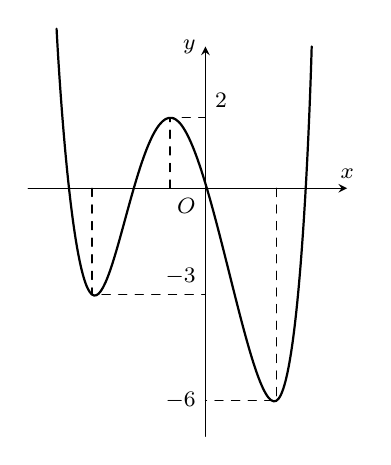
\begin{tikzpicture}[line join = round, line cap = round, >=stealth, font=\footnotesize, scale=0.45]
		%\tikzset{label style/.style={font=\footnotesize}}
		\draw[->] (-5,0)--(0,0) node[below left]{$O$} -- (4,0) node[above]{$x$};
		\draw[->] (0,-7) -- (0,4) node[left]{$y$};
		\draw[dashed] (-3.2,0)-- (-3.2,-3)--(0,-3)node[above left]{$-3$} (-1,0)--(-1,2)--(0,2)node[above right]{$2$} (2,0)--(2,-6)--(0,-6)node[left]{$-6$};
		\draw[thick] plot[smooth,tension=0.7] coordinates{(-4.2,4.5) (-3.2,-3) (-0.85,1.95) (2,-6) (3,4)};
	\end{tikzpicture}
	}
	\loigiai{
	\begin{center}
		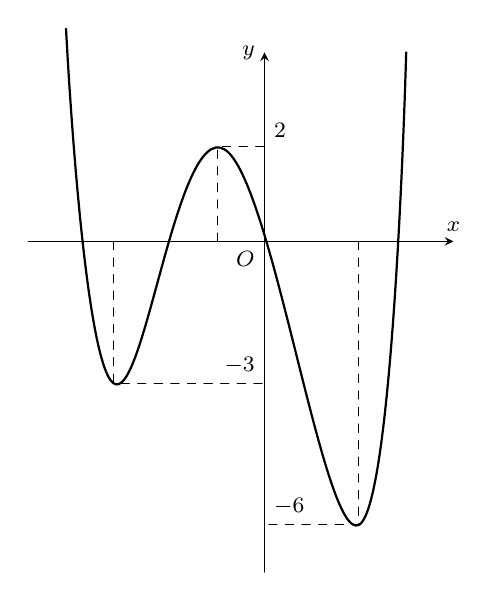
\begin{tikzpicture}[line join = round, line cap = round, >=stealth, font=\footnotesize, scale=0.6]
			%\tikzset{label style/.style={font=\footnotesize}}
			\draw[->] (-5,0)--(0,0) node[below left]{$O$} -- (4,0) node[above]{$x$};
			\draw[->] (0,-7) -- (0,4) node[left]{$y$};
			\draw[dashed] (-3.2,0)-- (-3.2,-3)--(0,-3)node[above left]{$-3$} (-1,0)--(-1,2)--(0,2)node[above right]{$2$} (2,0)--(2,-6)--(0,-6)node[above right]{$-6$};
			\draw[thick] plot[smooth,tension=0.7] coordinates{(-4.2,4.5) (-3.2,-3) (-0.85,1.95) (2,-6) (3,4)};
		\end{tikzpicture}
	\end{center}
	\textbf{Cách 1:} dùng đồ thị.\\
	Nhận thấy: số giao điểm của $(C)\colon y=f(x)$ với $Ox$ bằng số giao điểm của $\left(C_1\right):y=f\left(x-2\right)$ với $Ox$.\\
	Vì $m>0$ nên $\left(C_2\right)\colon y=f\left(x-2\right)+m$ có được bằng cách tịnh tiến $\left(C_1\right)\colon y=f\left(x-2\right)$ lên trên $m$ đơn vị.\\
	Đồ thị hàm số $y=\left|f\left(x-2\right)+m\right|$ có được bằng cách lấy đối xứng qua trục hoành $Ox$ phần đồ thị $\left(C_2\right)$ nằm phía dưới trục $Ox$ và giữ nguyên phần phía trên trục $Ox$ .\\
	Ta xét các trường hợp sau:
	\begin{center}
		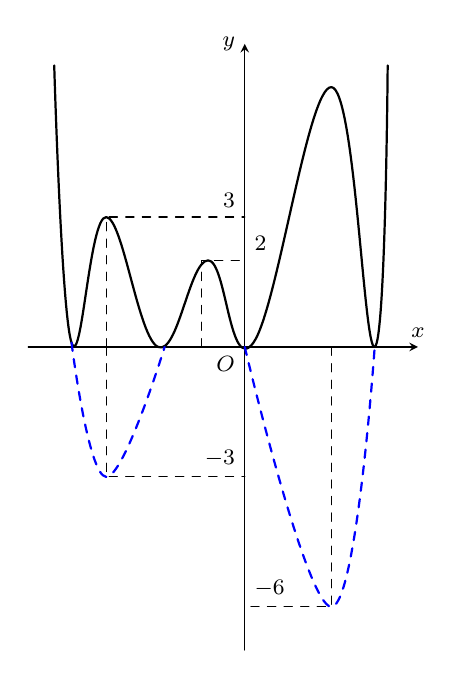
\begin{tikzpicture}[line join = round, line cap = round, >=stealth, font=\footnotesize, scale=0.55]
			%\tikzset{label style/.style={font=\footnotesize}}
			\draw[->] (-5,0)--(0,0) node[below left]{$O$} -- (4,0) node[above]{$x$};
			\draw[->] (0,-7) -- (0,7) node[left]{$y$};
			\draw[dashed] (-3.2,0)-- (-3.2,3)--(0,3)node[above left]{$3$}
			(-3.2,0)-- (-3.2,-3)--(0,-3)node[above left]{$-3$}
			(-1,0)--(-1,2)--(0,2)node[above right]{$2$}
			(2,0)--(2,-6)--(0,-6)node[above right]{$-6$};
			\draw[thick] plot[smooth,tension=0.7] coordinates{(-4.4,6.5) (-4,.1) (-3.2,3) (-2,0) (-0.85,2) (.2,.1) (2,6) (3,0) (3.3,6.5)};
			\draw[dashed,thick,blue] plot[smooth,tension=0.7] coordinates{ (-4,.1) (-3.2,-3) (-1.85,0)};
			\draw[dashed,thick,blue] plot[smooth,tension=0.7] coordinates{ (0,0) (2,-6) (3,0)};
		\end{tikzpicture}
		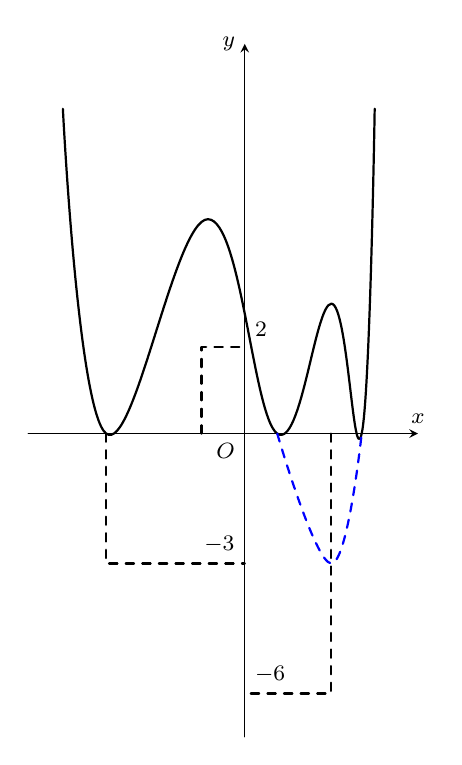
\begin{tikzpicture}[line join = round, line cap = round, >=stealth, font=\footnotesize, scale=0.55]
			%\tikzset{label style/.style={font=\footnotesize}}
			\draw[->] (-5,0)--(0,0) node[below left]{$O$} -- (4,0) node[above]{$x$};
			\draw[->] (0,-7) -- (0,9) node[left]{$y$};
			\draw[dashed,thick] (-3.2,0)-- (-3.2,-3)--(0,-3)node[above left]{$-3$} (-1,0)--(-1,2)--(0,2)node[above right]{$2$} (2,0)--(2,-6)--(0,-6)node[above right]{$-6$};
			\draw[thick] plot[smooth,tension=0.7] coordinates{(-4.2,7.5) (-3.2,0) (-0.85,4.95) (.75,0) (2,3) (2.7,0) (3,7.5)};
			\draw[dashed,thick,blue] plot[smooth,tension=0.7] coordinates{(.75,0) (2,-3) (2.7,0)};
		\end{tikzpicture}
		\begin{tikzpicture}[line join = round, line cap = round, >=stealth, font=\footnotesize, scale=0.55]
			%\tikzset{label style/.style={font=\footnotesize}}
			\draw[->] (-5,0)--(0,0) node[below left]{$O$} -- (4,0) node[above]{$x$};
			\draw[->] (0,-7) -- (0,11) node[left]{$y$};
			\draw[dashed] (-3.2,0)-- (-3.2,-3)--(0,-3)node[above left]{$-3$} (-1,0)--(-1,2)--(0,2)node[above right]{$2$} (2,0)--(2,-6)--(0,-6)node[above right]{$-6$};
			\draw[thick] plot[smooth,tension=0.7] coordinates{(-4.2,10.5) (-3.2,3) (-0.85,7.95) (2,0) (3,10.5)};
		\end{tikzpicture}
	\end{center}
	\begin{itemize}
		\item Trường hợp 1: $0<m<3$: đồ thị hàm số có $7$ điểm cực trị (loại).
		\item Trường hợp 2: $m=3$: đồ thị hàm số có $5$ điểm cực trị (thỏa mãn).
		\item Trường hợp 3: $3<m<6$: đồ thị hàm số có $5$ điểm cực trị (thỏa mãn).
		\item Trường hợp 4: $m\ge 6$: đồ thị hàm số có $3$ điểm cực trị (loại).
	\end{itemize}
	Vậy $3\le m<6$ Do $m\in\mathbb{Z}_+^*$ nên $m\in\left\{ 3;4;5\right\}$ hay $S=\left\{ 3;4;5\right\}$.\\
	Vậy tổng giá trị tất cả các phần tử của $S$ bằng $12$.\\
	\textbf{Cách 2:} đạo hàm hàm số hợp.\\
	Ta có: $y=\left|f\left(x-2\right)+m\right|$ $=\sqrt{\left[f\left(x-2\right)+m\right]^2}$ $\Rightarrow{y}'=\dfrac{\left(f\left(x-2\right)+m\right).f'\left(x-2\right)}{\sqrt{\left[f\left(x-2\right)+m\right]^2}}$\\
	Xét $f'\left(x-2\right)=0$ $(1)$\\
	Do phương trình $f'(x)=0$ có $3$ nghiệm phân biệt nên phương trình $f'\left(x-2\right)=0$ cũng có $3$ nghiệm phân biệt.\\
	-Xét $f\left(x-2\right)+m=0$ $\Leftrightarrow f\left(x-2\right)=-m$ $(2)$\\
	Nếu $-6<-m<-3$ $\Leftrightarrow 3<m<6$ thì phương trình $(2)$ có $2$ nghiệm phân biệt khác $3$ nghiệm của $(1)$.\\
	Nếu $-m=-3$ $\Leftrightarrow m=3$ thì $(2)$ có $3$ nghiệm phân biệt (trong đó có $2$ nghiệm đơn khác $3$ nghiệm của $(1)$ và $1$ nghiệm kép trùng với $1$ nghiệm của $(1)$)\\
	Tóm lại: với $3\le m<6$ thì hai phương trình $(1)$ và $(2)$ có tất cả $5$ nghiệm bội lẻ phân biệt và $y'$ đổi dấu khi $x$ đi qua các nghiệm đó, hay đồ thị hàm số $y=\left| f\left(x-2\right)+m\right|$ có $5$ điểm cực trị.\\
	-Lại do $m\in\mathbb{Z}_+^*$ nên $m\in\left\{ 3;4;5\right\}$ hay $S=\left\{3;4;5\right\}$.\\
	Vậy tổng giá trị tất cả các phần tử của $S$ bằng $12$.
}
\end{ex}
\begin{ex}[Sở Hưng Yên-2018]%Câu 17%[2D1G2-2]
	Cho hàm số $f(x)=\left|x^3-3x^2+m\right|$ với $m\in\left[-5;5\right]$ là tham số. Có bao nhiêu giá trị nguyên của $m$ để hàm số $f(x)$ có đúng ba điểm cực trị.
	\choice
	{$3$}
	{$0$}
	{\True $8$}
	{$6$}
	\loigiai{
	Xét hàm số $g(x)=x^3-3x^2+m$ có $g'(x)=0\Leftrightarrow 3x^2-6x=0\Leftrightarrow\left[\begin{aligned}
		&x=0\\
		&x=2\\
	\end{aligned}\right.$.\\
	Bảng biến thiên
	\begin{center}
		
\begin{tikzpicture}
			\tkzTabInit[nocadre,lgt=1.2,espcl=2.5]
			{$x$/0.8,$g'(x)$/0.8,$g(x)$/2.5}
			{$-\infty$,$0$,$2$,$+\infty$}
			\tkzTabLine{,+,0,-,0,+}
			\tkzTabVar{-/$-\infty$,+/$m$,-/$-4+m$,+/$+\infty$}
		\end{tikzpicture}
	\end{center}
	Từ bảng biến thiên ta thấy để hàm số $f(x)$ có đúng ba điểm cực trị thì đồ thị hàm số $g(x)$ phải có đúng một giao điểm hoặc tiếp xúc với $Ox$.\\
	Điều kiện này tương đương với $\left[\begin{aligned}
		&m\le 0\\
		&-4+m\ge 0\\
	\end{aligned}\right.\Leftrightarrow\left[\begin{aligned}
		&m\le 0\\
		&m\ge 4\\
	\end{aligned}\right.$. Kết hợp điều kiện $m\in\left[-5;5\right]$ ta có $m\in\left\{-5;-4;-3;-2;-1;0;4;5\right\}$. Vậy có 8 giá trị thoả mãn.
	}
\end{ex}
\begin{ex}[Chuyên Hùng Vương-Bình Dương-2018]%Câu 18%[2D1G2-2]
	Cho hàm số $y=f(x)$ có bảng biến thiên như sau.
	\begin{center}
		
\begin{tikzpicture}[thick,line cap=round,line join=round,font=\footnotesize]
			\tkzTabInit[nocadre,lgt=1.2,espcl=2.5]
			{$x$/0.8,$f'(x)$/0.8,$f(x)$/2.5}
			{$-\infty$,$-1$,$3$,$+\infty$}
			\tkzTabLine{,+,0,-,0,+}
			\tkzTabVar{-/$-\infty$,+/$2018$,-/$-2018$,+/$+\infty$}
		\end{tikzpicture}
	\end{center}
	Đồ thị hàm số $y=\left|f\left(x-2017\right)+2018\right|$ có bao nhiêu điểm cực trị?
	\choice
	{$2$}
	{\True $3$}
	{$5$}
	{$4$}
	\loigiai{
	Có $y=f\left(x-2017\right)$ bằng cách tịnh tiến sang bên phải $2017$ đơn vị ta có:\\
	bảng biến thiên của hàm số $y=f\left(x-2017\right)$.
	\begin{center}
		
\begin{tikzpicture}[thick,line cap=round,line join=round,font=\footnotesize]
			\tkzTabInit[nocadre,lgt=2.25,espcl=2.5]
			{$x$/0.8,$f(x-2017)$/2.5}
			{$-\infty$,$2016$,$2020$,$+\infty$}
			%\tkzTabLine{,+,0,-,0,+}
			\tkzTabVar{-/$-\infty$,+/$2018$,-/$-2018$,+/$+\infty$}
		\end{tikzpicture}
	\end{center}
	Tịnh tiến đồ thị hàm số $f\left(x-2017\right)$ lên trên 2018 đơn vị và lấy trị tuyệt đối ta có bảng biến thiên của hàm số $y=\left|f\left(x-2017\right)+2018\right|$.
	\begin{center}
		
\begin{tikzpicture}
			\tkzTabInit[nocadre,lgt=1.25,espcl=2.5]
			{$x$/0.8,$y$/2.5}
			{$-\infty$,,$2016$,$2020$,$+\infty$}
			%\tkzTabLine{,+,0,-,0,+}
			\tkzTabVar{+/$ $,-/$0$,+/$4036$,-/$0$,+/$ $}
		\end{tikzpicture}
	\end{center}
	Từ bảng biến thiên, suy ra hàm số có $3$ cực trị.
}
\end{ex}
\begin{ex}[Chuyên Ngữ-Hà Nội-2018]%Câu 19%[2D1G2-1]
Hàm số $f(x)$ có đạo hàm $f'(x)$ trên $\mathbb{R}$. Hình vẽ bên là đồ thị của hàm số $f'(x)$ trên $\mathbb{R}$.
\begin{center}
	\begin{tikzpicture}[join=round, cap=round, >=stealth, scale=1, thick]
		\draw[->] (-4,0)--(4,0)node[below]{$x$};
		\draw[->] (0,-2.5)--(0,5)node[left]{$y$};
		\draw [line width=1pt,blue ]
		(-3,-2) .. controls + (85:1.0) and + (-180:1.0) ..
		(-1.5,4) .. controls + (0:1.0) and + (-180:1.0) ..
		(1.5,-1) .. controls + (0:1.0) and + (-180:0.0) ..
		(3,4) ;
		\path
		%(-3,0) node[below left]{$-3$}
		%(-2,0) node[below left]{$-2$}
		%(-1,0) node[below left]{$-1$}
		(0,0) node[below left]{$O$} ;
		\foreach \diemx/\diemy in {-3/0,-2/0,-1/0, 0/0, 1/0,2/0,3/0, 0/-2,0/-1,0/1,0/2,0/3,0/4}
		\fill (\diemx,\diemy)circle(1.2pt);
	\end{tikzpicture}
\end{center}
	Hỏi hàm số $y=f\left(\left|x\right|\right)+2018$ có bao nhiêu điểm cực trị?
	\choice
	{\True $5$}
	{$3$}
	{$2$}
	{$4$}
	\loigiai{
	\textbf{Cách 1:} Từ đồ thị hàm số của $f'(x)$ ta thấy $f(x)$ có hai cực trị dương nên hàm số $y=f\left(\left| x\right|\right)$ lấy đối xứng phần đồ thị hàm số bên phải trục tung qua trục tung ta được bốn cực trị, cộng thêm giao điểm của đồ thị hàm số $y=f\left(\left| x\right|\right)+2018$ với trục tung nữa ta được tổng cộng là $5$ cực trị.\\
	\textbf{Cách 2:} Ta có: $y=f\left(\left|x\right|\right)+2018=f\left(\sqrt{x^2}\right)+2018$.\\
	Đạo hàm: $y'=f'\left(\sqrt{x^2}\right){\left(\sqrt{x^2}\right)'}=\dfrac{x}{\sqrt{x^2}}.f'\left(\left|x\right|\right)$.\\
	Từ đồ thị hàm số của $f'(x)$ suy ra $f'(x)$ cùng dấu với $\left(x-x_1\right)\left(x-x_2\right)\left(x-x_3\right)$ với $x_1<0$, $0<x_2<x_3$.\\
	Suy ra: $f'\left(\left|x\right|\right)$ cùng dấu với $\left(\left|x\right|-x_1\right)\left(\left|x\right|-x_2\right)\left(\left|x\right|-x_3\right)$.\\
	Do $\left| x\right|-x_1>0$ nên $y'=f'\left(\sqrt{x^2}\right){\left(\sqrt{x^2}\right)'}=\dfrac{x}{\sqrt{x^2}}{f}'\left(\left| x\right|\right)$ cùng dấu với $\left(\left| x\right|-x_2\right)\left(\left|x\right|-x_3\right).\dfrac{x}{\sqrt{x^2}}$.\\
	Vậy hàm số $y=f\left(\left|x\right|\right)+2018$ có $5$ cực trị.
}
\end{ex}
\begin{ex}[Sở-Nam Định-2018]%Câu 20%[2D1G2-2]
Cho hàm số $y=f(x)$ có bảng biến thiên như hình vẽ
\begin{center}
	
\begin{tikzpicture}[thick,font=\footnotesize,line cap=round,line join=round]
		\tkzTabInit[nocadre,lgt=1.2,espcl=2.5]
		{$x$/0.8,$f'(x)$/0.8,$f(x)$/2.5}
		{$-\infty$,$1$,$2$,$+\infty$}
		\tkzTabLine{,+,0,-,0,+}
		\tkzTabVar{-/$-\infty$,+/$11$,-/$4$,+/$+\infty$}
	\end{tikzpicture}
\end{center}
	Đồ thị hàm số $y=\left|f(x)-2m\right|$ có $5$ điểm cực trị khi và chỉ khi
	\choice
	{$m\in\left(4;11\right)$}
	{\True $m\in\left(2;\dfrac{11}{2}\right)$}
	{$m=3$}
	{$m\in\left[2;\dfrac{11}{2}\right]$}
	\loigiai{
	Từ bảng biến thiên ta có đồ thị hàm số $y=f(x)$ có hai điểm cực trị.\\
	Để đồ thị hàm số $y=\left|f(x)-2m\right|$ có $5$ điểm cực trị thì đồ thị $y=f(x)$ cắt đường thẳng $y=2m$ tại $5-2=3$ điểm phân biệt $\Leftrightarrow 4<2m<11\Leftrightarrow 2<m<\dfrac{11}{2}$.
	}
\end{ex}
\begin{ex}[Sở Hưng Yên-2021]%Câu 21%[2D1G2-1]
	Gọi $X$ là tập hợp các số nguyên $m\in\left[-2021;2021\right]$ sao cho đồ thị hàm số $y=\left|x^3-\left(2m+1\right){x^2}+mx+m\right|$ có $5$ điểm cực trị. Tổng các phần tử của $X$ là
	\choice
	{$0$}
	{$4036$}
	{\True $1$}
	{$-1$}
	\loigiai{
	Xét hàm số $f(x)=x^3-\left(2m+1\right){x^2}+mx+m$.\\
	Ta có $f'(x)=3x^2-2\left(2m+1\right)x+m$.\\
	$\Delta'=\left(2m+1\right)^2-3m=3m^2+\left(m+\dfrac{1}{2}\right)^2+\dfrac{3}{4}>0$, với mọi $m\in\mathbb{R}$.\\
	Suy ra hàm số $f(x)$ luôn có $2$ điểm cực trị, với mọi $m\in\mathbb{R}$.\\
	$f(x)=0\Leftrightarrow{x^3}-\left(2m+1\right){x^2}+mx+m=0$ $(1)$\\
	$\Leftrightarrow\left(x-1\right)\left(x^2-2mx-m\right)=0$ $\Leftrightarrow\left[\begin{aligned}
		&x=1\\
		&{x^2}-2mx-m=0~(2)\\
	\end{aligned}\right.$.\\
	Hàm số đã cho có $5$ điểm cực trị $\Leftrightarrow$ phương trình $(1)$ có $3$ nghiệm phân biệt.\\
	$\Leftrightarrow$ phương trình $(2)$ có $2$ nghiệm phân biệt, khác $1$.\\
	$\Leftrightarrow\left\{\begin{aligned}
		&{\Delta}'=m^2+m>0\\
		& 1-3m\ne 0\\
	\end{aligned}\right.$ $\Leftrightarrow\left\{\begin{aligned}
		&\left[\begin{aligned}
			& m<-1\\
			& m>0\\
		\end{aligned}\right.\\
		& m\ne\dfrac{1}{3}\\
	\end{aligned}\right.$.\\
	Vì $m\in\mathbb{Z}$ và $m\in\left[-2021;2021\right]$ nên $m\in\left\{\pm 2021;\pm 2020;\ldots;\pm 2;1\right\}$.\\
	Suy ra $X=\left\{\pm 2021;\pm 2020;\ldots;\pm 2;1\right\}$.\\
	Vậy tổng các phần tử của tập $X$ bằng $1$.
}
\end{ex}
\begin{ex}[Mã 101-2022]%Câu 22%[2D1G2-2]
	Có bao nhiêu giá trị nguyên dương của tham số $m$ để hàm số $y=\left|x^4-2m{x^2}+64x\right|$ có đúng ba điểm cực trị
	\choice
	{\True $5$}
	{$6$}
	{$12$}
	{$11$}
	\loigiai{
	Xét hàm số $y=x^4-2m{x^2}+64x$.\\
	Ta có: $y'=4x^3-4mx+64~(*)$.\\
	Phương trình hoành độ giao điểm: $x^4-2m{x^2}+64x=0\Leftrightarrow\left[\begin{aligned}
		&x=0\\
		&{x^3}-2mx+64=0~(1)\\
	\end{aligned}\right.$.\\
	Phương trình $(1)$ luôn có một nghiệm $x\ne 0$ nên đồ thị hàm số $y=x^4-2m{x^2}+64x$ cắt $Ox$ ít nhất hai điểm và $\underset{x\to\pm\infty}{\lim}\left(x^4-2m{x^2}+64x\right)=+\infty $.\\
	Suy ra để hàm số $y=\left|x^4-2m{x^2}+64x\right|$ có $3$ điểm cực trị thì hàm số $y=x^4-2m{x^2}+64x$ có đúng một điểm cực trị $\Leftrightarrow $ phương trình $(*)$ có đúng một nghiệm đơn.\\
	$m=x^2+\dfrac{16}{x}$ có đúng một nghiệm đơn.\\
	Xét hàm số: $f(x)=x^2+\dfrac{16}{x}$, $f'(x)=2x-\dfrac{16}{x^2}$.\\
	$f'(x)=0\Leftrightarrow 2x-\dfrac{16}{x^2}=0\Leftrightarrow x=2$.\\
	Bảng biến thiên:
	\begin{center}
		
\begin{tikzpicture}[scale=1,font=\footnotesize,line width=1pt]
			\tkzTabInit[nocadre,lgt=1.2,espcl=2.5]
			{$x$/0.8,$f'(x)$/0.8,$f(x)$/2.5}
			{$-\infty$,$0$,$2$,$+\infty$}
			\tkzTabLine{,-,d,-,0,+,}
			\tkzTabVar{+/$+\infty$,-D+/$-\infty$/$+\infty$,-/$12$,+/$+\infty$}
		\end{tikzpicture}
	\end{center}
	Từ bảng biến thiên suy ra $m\le 12$.\\
	Suy ra: $\left\{\begin{aligned}
		&m\in\mathbb{Z}_+^*\\
		&m\le 12\\
	\end{aligned}\right.\Rightarrow m\in\left\{1;2;3;\ldots;11;12\right\}$.\\
	Vậy có $12$ giá trị nguyên dương của tham số $m$ để hàm số $y=\left|x^4-2m{x^2}+64x\right|$ có đúng ba điểm cực trị.
}
\end{ex}
\begin{ex}[Mã 102-2022]%Câu 23%[2D1G2-2]
	Có bao nhiêu giá trị nguyên âm của tham số $a$ để hàm số $y=\left|x^4+2a{x^2}+8x\right|$ có đúng ba điểm cực trị?
	\choice
	{$2$}
	{$6$}
	{$5$}
	{\True $3$}
	\loigiai{
	Xét hàm số $f(x)=x^4+2a{x^2}+8x$ trên $\mathbb{R}$.\\
	$f'(x)=4x^3+4ax+8$.\\
	$f'(x)=0$ $\Leftrightarrow 4x^3+4ax+8=0\Leftrightarrow a=-x^2-\dfrac{2}{x}$ (Do $x=0$ không thỏa mãn nên $x\ne 0$).\\
	Xét hàm số $g(x)=-x^2-\dfrac{2}{x}$ trên $\mathbb{R}\setminus\left\{ 0\right\}$.\\
	$g'(x)=-2x+\dfrac{2}{x^2}$.\\
	$f'(x)=0$ $\Leftrightarrow $ $-2x+\dfrac{2}{x^2}=0$ $\Leftrightarrow $ $x=1$ .\\
	Bảng biến thiên của hàm số $g(x)$:
	\begin{center}
		
\begin{tikzpicture}[scale=1,thick,font=\footnotesize]
			\tkzTabInit[nocadre,lgt=1.2,espcl=2.5]
			{$x$/0.8,$g'(x)$/0.8,$g(x)$/2.5}
			{$-\infty$,$0$,$1$,$+\infty$}
			\tkzTabLine{,+,d,+,0,-,}
			\tkzTabVar{-/$-\infty$,+D-/$+\infty$/$-\infty$,+/$-3$,-/$-\infty$}
		\end{tikzpicture}
	\end{center}
	Dễ thấy phương trình $f(x)=0$ có ít nhất hai nghiệm phân biệt, trong đó có ít nhất một nghiệm đơn $x=0$ nên yêu cầu bài toán $\Leftrightarrow$ Hàm số $f(x)$ có đúng một điểm cực trị $\Leftrightarrow$ Phương trình $a=g(x)$ có một nghiệm đơn duy nhất $\Leftrightarrow$ $a\ge-3$.\\
	Do $a$ nguyên âm nên $a\in\left\{-3;-2;-1\right\}$.\\
	Vậy có $3$ giá trị nguyên âm của tham số $a$ thỏa mãn yêu cầu bài toán.
}
\end{ex}
\begin{ex}[Mã 103-2022]%Câu 24%[2D1G2-2]
	Có bao nhiêu giá trị nguyên âm của tham số $a$ để hàm số $y=\left|x^4+a{x^2}-8x\right|$ có đúng 3 điểm cực trị?
	\choice
	{$5$}
	{\True $6$}
	{$11$}
	{$10$}
	\loigiai{
	Xét $g(x)=x^4+a{x^2}-8x$.\\
	$g'(x)=4x^3+2ax-8$.\\
	Xét $g'(x)=0\Leftrightarrow 4x^3+2ax-8=0\Leftrightarrow-a=\dfrac{2x^3-4}{x}=2x^2-\dfrac{4}{x}=h(x)$ (do $x=0$ không là nghiệm).\\
	$g(x)=0\Leftrightarrow\left[\begin{aligned}
		&x=0\\
		&{x^3}+ax-8=0\Leftrightarrow-a=\dfrac{x^3-8}{x}=x^2-\dfrac{8}{x}=k(x)\\
	\end{aligned}\right.$\\
	$h'(x)=4x+\dfrac{4}{x^2}=0\Leftrightarrow x=-1$.\\
	$k'(x)=2x+\dfrac{8}{x^2}=0\Leftrightarrow x=\sqrt[3]{-4}$.
	\begin{center}
		\begin{tikzpicture}[scale=1,>=stealth,font=\footnotesize,line width=.8pt]
			\tkzTabInit[nocadre,lgt=1.5,espcl=2.5]
			{$x$/0.8,$h(x)$/2.5,$k(x)$/2.5}
			{$-\infty$,$\sqrt[3]{-4}$,$-1$,$0$,$+\infty$}
			\tkzTabLine{}
			\tkzTabVar{}
			\path (N11) node[below](A){$+\infty$}
			(N32) node[above](C){$6$}
			(barycentric cs:A=1,C=1) node(B){$h(\sqrt[3]{-4})$}
			(N41) node[below left](D){$+\infty$}
			(N42) node[above right](E){$-\infty$}
			(N51) node[below](F){$+\infty$}
			(N12) node[below](a){$+\infty$}
			(N23) node[above](b){$k(\sqrt[3]{-4})$}
			(N42) node[below left](d){$+\infty$}
			(barycentric cs:b=1,d=1) node(c){$9$}
			(N43) node[above right](e){$-\infty$}
			(N52) node[below](f){$+\infty$}
			;
			\draw[double] (N41)--(N43);
			\draw[->] (A)--(B);
			\draw[->] (B)--(C);
			\draw[->] (C)--(D);
			\draw[->] (E)--(F);
			\draw[->] (a)--(b);
			\draw[->] (b)--(c);
			\draw[->] (c)--(d);
			\draw[->] (e)--(f);
		\end{tikzpicture}
	\end{center}
	Để hàm số $y=\left|g(x)\right|$ có đúng $3$ cực trị $\Leftrightarrow-a\le 6\Leftrightarrow a\ge-6$.\\
	Mà $a$ là số nguyên âm nên $a\in\left\{-6;-5;-4;-3;-2;-1\right\}$.
}
\end{ex}
\begin{ex}[Mã 104-2022]%Câu 25%[2D1G2-2]
	Có bao nhiêu số nguyên dương của tham số $m$ để hàm số $y=\left|x^4-m{x^2}-64x\right|$ có đúng $3$ điểm cực trị?
	\choice
	{$23$}
	{$12$}
	{\True $24$}
	{$11$}
	\loigiai{
	Xét hàm số $g(x)=x^4-m{x^2}-64x$; $g'(x)=4x^3-2mx-64$; có $\underset{x\to\pm\infty}{\lim}f(x)=+\infty$.\\
	$g(x)=0\Leftrightarrow\left[\begin{aligned}
		&x=0\\
		&{x^3}-mx-64=0\\
	\end{aligned}\right.\Rightarrow g(x)=0$ có ít nhất $2$ nghiệm phân biệt.\\
	Do đó hàm số $y=\left|g(x)\right|$ có đúng $3$ điểm cực trị $\Leftrightarrow$ hàm số $y=g(x)$ có đúng 1 cực trị $\Leftrightarrow g'(x)$ đổi dấu đúng $1$ lần $(*)$.\\
	Nhận xét nếu $x=0\Rightarrow{g}'(0)=-64<0$ $\Rightarrow g(x)$ không có cực trị (hay $x=0$ không thỏa mãn).\\
	Nên $g'(x)=0\Leftrightarrow m=2x^2-\dfrac{32}{x}$. Đặt $h(x)=2x^2-\dfrac{32}{x}$.\\
	Có $h'(x)=4x+\dfrac{32}{x^2}=\dfrac{4\left(x^3+8\right)}{x^2}$; $h'(x)=0\Leftrightarrow x=-2$.\\
	Bảng biến thiên
	\begin{center}
		
\begin{tikzpicture}[scale=1,font=\footnotesize,line width=.8pt]
			\tkzTabInit[nocadre,lgt=1.2,espcl=2.5]
			{$x$/0.8,$h'(x)$/0.8,$h(x)$/2.5}
			{$-\infty$,$-2$,$0$,$+\infty$}
			\tkzTabLine{,-,0,+,d,+,}
			\tkzTabVar{+/$+\infty$,-/$24$,+D-/$+\infty$/$-\infty$,+/$+\infty$}
		\end{tikzpicture}
	\end{center}
	Từ bảng biến thiên suy ra $(*)\Leftrightarrow m\le 24$ .\\
	Kết hợp với điều kiện $m$ nguyên dương suy ra $m\in\left\{1;2;3;\ldots;24\right\}$.
}
\end{ex}
\begin{ex}[Liên trường Hà Tĩnh – 2022]%Câu 26%[2D1G2-2]
	Cho hàm số $f(x)=x^4-14x^3+36x^2+(16-m)x$ với $m$ là tham số thực. Có bao nhiêu giá trị nguyên của $m$ để hàm số $g(x)=f(|x|)$ có $7$ điểm cực trị?
	\choice
	{\True $33$}
	{$31$}
	{$32$}
	{$34$}
	\loigiai{
	Xét hàm số: $f(x)=x^4-14x^8+36x^2+(16-m)x$.\\
	Tập xác định: $\mathscr{D}=\mathbb{R}$.\\
	$f'(x)=4x^8-42x^2+72x+16-m$.\\
	Hàm số $g(x)=f(|x|)$ có $7$ điểm cực trị $\Leftrightarrow$ Hàm số $f(x)$ có $3$ điểm cực trị dương.\\
	$\Leftrightarrow$ Phương trình $f'(x)=0$ có $3$ nghiệm dương phân biệt.\\
	Xét phương trình $f\prime (x)=0\Leftrightarrow 4x^3-42x^2+72x+16=m$ $(1)$.\\
	Đặt $h(x)=4x^8-42x^2+72x+16\Rightarrow h'(x)=12x^2-84x+72\Rightarrow h'(x)=0\Leftrightarrow\left[\begin{aligned}
		&x=1\\
		&x=6\\
	\end{aligned}\right.$.\\
	Ta có bảng biến thiên
	\begin{center}
		\begin{tikzpicture}[scale=1,font=\footnotesize,line width=.8pt,>=stealth]
			\tkzTabInit[nocadre,lgt=1.2,espcl=2.5]
			{$x$/0.8,$h'(x)$/0.8,$h(x)$/2.5}
			{$0$,$1$,$\fbox{6}$,$+\infty$}
			\tkzTabLine{,+,0,-,0,+}
			\tkzTabVar{%-/$16$,+/$50$,-/$-200$,+/$+\infty$
			}
			\path($(N13)+(0,.3)$) node[above](A){$\fbox{16}$}
			($(N22)+(0,-.3)$) node[below](B){$\fbox{50}$}
			(N33) node[above](C){\fbox{$-200$}}
			(N42) node[below](D){$+\infty$}
			;
			\draw[->] (A)--(B);
			\draw[->] (B)--(C);
			\draw[->] (C)--(D);
		\end{tikzpicture}
	\end{center}
	Yêu cầu bài toán $\Leftrightarrow (1)$ có $3$ nghiệm dương phân biệt khi và chỉ khi đường thẳng $y=m$ cắt đồ thị hàm số $y=h(x)$ tại $3$ điểm phân biệt có hoành độ dương.\\
	Dựa vào bảng biến thiên ta có $16<m<50$.\\
	Vì $m$ là số nguyên nên $m\in\left\{17;18;\ldots;49\right\}$ nên có $33$ số nguyên.
}
\end{ex}
\begin{ex}[Sở Thanh Hóa 2022]%Câu 27%[2D1G2-2]
	Cho hàm số $f(x)$ có đạo hàm liên tục trên $\mathbb{R}$ và $f(0)<0$, đồ thị của $f'(x)$ như hình vẽ:
	\begin{center}
		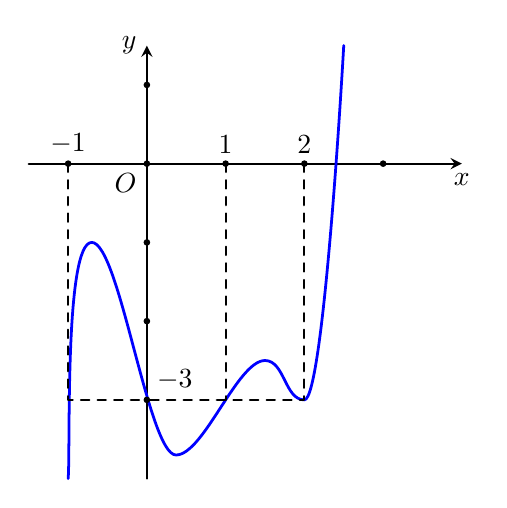
\begin{tikzpicture}[line join=round, line cap=round, >=stealth, scale=1, thick]
			\draw[->] (-1.5,0)--(4,0)node[below]{$x$};
			\draw[->] (0,-4)--(0,1.5)node[left]{$y$};
			\draw [line width=1pt,blue ]
			(-1,-4) .. controls + (85:.35) and + (-180:.35) ..
			(-0.7,-1) .. controls + (0:.35) and + (-180:.35) ..
			(0.37,-3.7) .. controls + (0:.35) and + (-180:.35) ..
			(1.5,-2.5) .. controls + (0:.25) and + (180:.25) ..
			(2,-3) .. controls + (0:.25) and + (-180:.0) ..
			(2.5,1.5);
			\draw[dashed] (-1,0)--(-1,-3)--(0,-3) (1,0)--(1,-3) (2,0)--(2,-3)--(0,-3)
			;
			\path
			(-1,0) node[above]{$-1$}
			(1,0) node[above]{$1$}
			(2,0) node[above]{$2$}
			(0,-3) node[above right]{$-3$}
			(0,0) node[below left]{$O$} ;
			\foreach \diemx/\diemy in {-1/0,0/0,1/0,2/0,3/0, 0/-3,0/-2,0/-1,0/1}
			\fill (\diemx,\diemy)circle(1.2pt);
		\end{tikzpicture}
	\end{center}
	Gọi $m$, $n$ lần lượt là số điểm cực đại, số điểm cực tiểu của hàm số $g(x)=|f(|x|)+3|x||$. Giá trị của $m^n$ bằng
	\choice
	{$4$}
	{\True $8$}
	{$27$}
	{$16$}
	\loigiai{
	Xét hàm số $u(x)=f(|x|)+3|x|$ là một hàm số chẵn nên chỉ cần xét trên $[0;+\infty)$ đế suy ra bảng biến thiên của $u(x)$ trên cả $\mathbb{R}$. Với $x\ge 0\Rightarrow u(x)=f(x)+3x\Rightarrow u'(x)=f'(x)+3=0\Leftrightarrow f'(x)=-3\overset{x\ge 0}{\longleftrightarrow}x=0;x=1;x=2$.\\
	Bảng biến thiên:
	\begin{center}
		\begin{tikzpicture}[line cap=round, line join=round, font=\footnotesize, >=stealth, scale=1, thick]
			\tkzTabInit[nocadre,lgt=1.2,espcl=2]
			{$x$/0.8,$u'(x)$/0.8,$u(x)$/3}
			{$-\infty$,$-2$,$-1$,$0$,$1$,$2$,$+\infty$}
			\tkzTabLine{,-,0,-,0,+,0,-,0,+,0,+}
			\tkzTabVar{%+/$+\infty$,R,-/$u(-1)$,+/$f(0)$,-/$u(1)$,R,+/$+\infty$
			}
			\path (N12) node[below](A){$+\infty$}
			(N33) node[above](B){$u(-1)$}
			($(N42)!.35!(N43)$) node[below](C){$f(0)<0$}
			(N53) node[above](D){$u(1)$}
			(N72) node[below](E){$+\infty$}
			;
			\draw[->] (A)--(B);
			\draw[->] (B)--(C);
			\draw[->] (C)--(D);
			\draw[->] (D)--(E);
			\draw[dashed] ($(N12)!.3!(N13)$)--($(N72)!.3!(N73)$) node[below left]{$y=0$};
		\end{tikzpicture}
	\end{center}
	Trong đó $u(-1)=u(1)=f(1)+3; u(0)=f(0)<0$.\\
	Suy $g(x)=|u(x)|$ có tất cả $5$ điểm cực trị trong đó $2$ điểm cực đại và $3$ điểm cực tiểu.
}
\end{ex}
\begin{ex}[THPT Lương Tài 2-Bắc Ninh-2022]%Câu 28%[2D1G2-2]
	Cho hàm số$y=f(x)=2x^3+b{x^2}+cx+d$ thỏa mãn $4b+2c+d+16<0$ và $9b-3c+d>54$. Hàm số $y=\left|f(x)\right|$ có tất cả bao nhiêu điểm cực trị?
	\choice
	{$2$}
	{$3$}
	{\True $5$}
	{$4$}
	\loigiai{
	Ta có $y=f(x)=2x^3+b{x^2}+cx+d$ liên tục trên$\mathbb{R}$. Vì $f(2)=4b+2c+d+16<0$, $f\left(-3\right)=9b-3c+d-54>0$, $\underset{x\to-\infty}{\lim}f(x)=-\infty$, $\underset{x\to+\infty}{\lim}f(x)=+\infty$ nên phương trình $f(x)=0$ có ba nghiệm phân biệt $x_1<-3<x_2<2<x_3$\\
	Suy ra $y=f(x)$ có hai điểm cực trị $x_1<m<x_2<n<x_3$.\\
	Ta có bảng biến thiên
	\begin{center}
		\begin{tikzpicture}[scale=1,font=\footnotesize,line width=1pt,>=stealth]
			\tkzTabInit[nocadre,lgt=1.5,espcl=2]
			{$x$/0.8,$f'(x)$/0.8,$f(x)$/2.5,$|f(x)|$/2.5}
			{$-\infty$,$x_1$,$m$,$x_2$,$n$,$x_3$,$+\infty$}
			\tkzTabLine{,,+,,0,,-,,0,,+}
			\tkzTabVar{%-/$-\infty$,R,+/$ $,R,-/$ $,R,+/$+\infty$
			}
			\tkzTabVar{+/,-/,+/,-/,+/,-/,+/}
			\path (N13) node[above](A){$-\infty$}
			(N32) node[below](B){}
			(N53) node[above](C){}
			(N72) node[below](D){$+\infty$}
			(barycentric cs:A=1,B=1) node(mAB){$0$}
			(barycentric cs:B=1,C=1) node(mBC){$0$}
			(barycentric cs:C=1,D=1) node(mCD){$0$}
			;
			\draw[->,blue] (A)--(mAB)--(B);
			\draw[->,blue] (B)--(mBC)--(C);
			\draw[->,blue] (C)--(mCD)--(D);
		\end{tikzpicture}
	\end{center}
	Vậy hàm số $y=\left| f(x)\right|$ có $5$ điểm cực trị.
}
\end{ex}
\begin{ex}[Chuyên Bắc Ninh 2022]%Câu 29%[2D1G2-1]
	Gọi $S$ là tập giá trị nguyên $m\in\left[0;100\right]$ để hàm số $y=\left|x^3-3m{x^2}+4m^3-12m-8\right|$ có $5$ cực trị. Tính tổng các phần tử của $S$.
	\choice
	{$10096$}
	{$4048$}
	{\True $5047$}
	{$10094$}
	\loigiai{
	Xét hàm số $f(x)=x^3-3m{x^2}+4m^3-12m-8$ trên $\mathbb{R}$.\\
	Ta có $f'(x)=3x^2-6mx$.\\
	$f'(x)=0\Leftrightarrow\left[\begin{aligned}
		&x=0\\
		&x=2m\\
	\end{aligned}\right.$.\\
	Hàm số $y=\left|x^3-3m{x^2}+4m^3-12m-8\right|$ có $5$ cực trị $\Leftrightarrow f(x)$ có hai giá trị cực trị trái dấu$\Leftrightarrow \Leftrightarrow\left\{\begin{aligned}
		&m\ne 0\\
		&\left(4m^3-12m-8\right)\left(8m^3-12m^3+4m^3-12m-8\right)<0\\
	\end{aligned}\right.$.\\
	$\Leftrightarrow\left\{\begin{aligned}
		&m\ne 0\\
		&\left(4m^3-12m-8\right)\left(-12m-8\right)<0\\
	\end{aligned}\right.$.\\
	Kết hợp với $m\in\left[0;100\right]$ và $m\in\mathbb{Z}$ ta được $m\in\left\{ 3;4;\ldots,100\right\}$.\\
	Vậy $S=\left\{ 3,4,\ldots,100\right\}$.\\
	Tổng các phần tử của $S$ là $5047$.
}
\end{ex}
\begin{ex}[Chuyên Quang Trung-Bình Phước 2022]%Câu 30%[2D1G2-2]
	Cho hàm số $f(x)=x^3+m{x^2}+nx-1$ với $m$, $n$ là các tham số thực thỏa mãn $\left\{\begin{aligned}
		&m+n>0\\
		&7+2(2m+n)<0\\
	\end{aligned}\right.$\\
	Tìm số cực trị của hàm $y=\left|f\left(\left|x\right|\right)\right|$.
	\choice
	{$2$}
	{$5$}
	{$9$}
	{\True $11$}
	\loigiai{
	Ta có $f(x)=x^3+m{x^2}+nx-1$ là hàm đa thức nên liên tục trên $\mathbb{R}$,\\ mặt khác $\left\{\begin{aligned}
		&f(1)=m+n>0\\
		&f(2)=7+2(2m+n)<0\\
	\end{aligned}\right.\Rightarrow f(1).f(2)<0$ suy ra $f(x)=0$ có ít nhất một nghiệm thuộc khoảng $\left(1;2\right)$.\\
	Ta có $\underset{x\to-\infty}{\mathop{{lim}}}f(x)=-\infty ;\underset{x\to+\infty}{\mathop{{lim}}}f(x)=+\infty $ ta có bảng biến thiên của hàm $y=f(x)$.
	\begin{center}
		\begin{tikzpicture}[line cap=round, line join=round, font=\footnotesize, scale=1, thick, >=stealth]
			\tkzTabInit[nocadre,lgt=1.2,espcl=1.5]
			{$x$/0.8,$f(x)$/3}
			{$-\infty$,,$1$,,$2$,,$+\infty$}
			%\tkzTabLine{,+,0,-,0,+}
			\tkzTabVar{%-/$-\infty$,+/$2$,-/$-2$,+/$+\infty$
			}
			\path (N12) node[above](A){$-\infty$}
			(N41) node[below](B){}
			(N62) node[above](C){}
			(N71) node[below](D){$+\infty$}
			($(barycentric cs:A=1,B=2)+(0,-.3)$) node(a){$f(1)$}
			($(intersection of B--C and N51--N52)+(0,-.3)$) node(b){$f(2)$}
			;
			\draw[->] (A)--(B);
			\draw[->] (B)--(C);
			\draw[->] (C)--(D);
			\draw[dashed,cyan] ($(N11)!.4!(N12)$)--($(N71)!.4!(N72)$) node[below,black]{$y=0$};
			\draw[thin,cyan] (N31)--(a) (N51)--(b);
		\end{tikzpicture}
	\end{center}
	Hàm số $y=f(x)$ có $2$ cực trị dương nên hàm số $y=f\left(\left|x\right|\right)$ có $5$ cực trị.\\ Mặt khác, đồ thị hàm số $y=f\left(\left|x\right|\right)$ cắt trục $Ox$ tại $6$ điểm. Suy ra hàm số $y=\left|f\left(\left|x\right|\right)\right|$ có $11$ cực trị.
}
\end{ex}
\begin{ex}[THPT Đồng Lộc-Hà Tĩnh 2022]%Câu 31%[2D1G2-2]
	Cho hàm số $y=f(x)=\left(x-1\right)g(x)$ có bảng biến thiên như sau
	\begin{center}
		
\begin{tikzpicture}
			\tkzTabInit[nocadre,lgt=1.2,espcl=2.5]
			{$x$/0.8,$f'(x)$/0.8,$f(x)$/2.5}
			{$-\infty$,$0$,$2$,$+\infty$}
			\tkzTabLine{,+,0,-,0,+}
			\tkzTabVar{-/$-\infty$,+/$2$,-/$-2$,+/$+\infty$}
		\end{tikzpicture}
	\end{center}
	Đồ thị hàm số $y=\left|x-1\right|g(x)$ có bao nhiêu điểm cực trị?
	\choice
	{$1$}
	{$4$}
	{$2$}
	{\True $3$}
	\loigiai{
	Ta có $y=\left|x-1\right|g(x)=\left\{\begin{aligned}
		&\left(x-1\right)g(x){khi}x\ge 1\\
		&-\left(x-1\right)g(x){khi}x<1\\
	\end{aligned}\right.$ hay $y=\left|x-1\right|g(x)=\left\{\begin{aligned}
		& f(x){khi}x\ge 1\\
		&-f(x){khi}x<1\\
	\end{aligned}\right.$.\\
	Dựa vào đồ thị hàm số $y=f(x)=\left(x-1\right)g(x)$ ta có bảng biến thiên của hàm số $y=\left|x-1\right|g(x)$ như sau:
	\begin{center}
		\begin{tikzpicture}[thick,>=stealth,line cap=round, line join=round]
			\tkzTabInit[nocadre,lgt=1.2,espcl=2]
			{$x$/0.8,$f(x)$/3}
			{$-\infty$,,$0$,$1$,$2$,,$+\infty$}
			%\tkzTabLine{,+,0,-,0,+}
			\tkzTabVar{%+/$+\infty$,R,-/$-2$,+/,-/$-2$,R,+/$+\infty$
			}
			\path(N11) node[below](A){$+\infty$}
			(N32) node[above](B){$-2$}
			(barycentric cs:N31=1,N52=1) node(C){}
			(N52) node[above](D){$-2$}
			(N71) node[below](E){$+\infty$}
			(N12) node[above](a){$-\infty$}
			(N31) node[below](b){$2$}
			(N51) node[below](c){$2$}
			;
			\draw[->,red] (A)--(B);
			\draw[->,red] (B)--(C)--(D);
			\draw[->,red] (D)--(E);
			\draw[->,dashed,blue] (a)--(b);
			\draw[dashed,blue] (C)--(b);
			\draw[dashed,red] (barycentric cs:N11=1,N12=1)--(barycentric cs:N71=1,N72=1);
		\end{tikzpicture}
	\end{center}
	Do đó, đồ thị hàm số $y=\left| x-1\right|g(x)$ có $3$ điểm cực trị.
	}
\end{ex}
\begin{ex}[THPT Nguyễn Viết Xuân – Vĩnh Phúc 2022]%Câu 32%[2D1G2-1]
	Cho hàm số $y=f(x)$ liên tục trên tập $\mathbb{R}$, biết $f'(x)=x^{2022}(x-2)^{2021}\left(x^2-8 x+m^2-3 m-4\right),\quad\forall x\in \mathbb{R}$. Gọi $S$ là tập tất cả các giá trị nguyên của $m$ để đồ thị hàm số $y=f(|x|)$ có $5$ điểm cực trị. Số phần tử của $S$ là:
	\choice
	{$7$}
	{\True $6$}
	{$4$}
	{$5$}
	\loigiai{
	$f'(x)=x^{2022}{(x-2)^{2021}}\left(x^2-8x+m^2-3m-4\right)=x^{2022}{(x-2)^{2020}}(x-2)\left(x^2-8x+m^2-3m-4\right)$.\\
	Để hàm số $y=g(x)=f(|x|)$ có $5$ điểm cực trị thì đồ thị hàm số $y=f(x)$ có 2 cực trị dương.\\
	Ta có $f'(x)=0\Leftrightarrow\left[\begin{aligned}
		&x=0\\
		&x=2\\
		&x^2-8 x+m^2-3 m-4=0~(1)\\
	\end{aligned}\right.$\\
	Có $x=0$ là nghiệm bội $2$, $x=2$ là nghiệm đơn.\\
	Vậy $x^2-8x+m^2-3m-4=0$ $(1)$ có hai nghiệm phân biệt, có một nghiệm dương $x\neq 2$, có một nghiệm $x\leq 0$\\
	\textbf{Trường hợp 1:} Có nghiệm $x=0$ khi đó $m^2-3m-4=0\Leftrightarrow\left[\begin{aligned}
		&m=-1\\
		&m=4\\
	\end{aligned}\right.$.\\
	Với $m=-1$, $m=4$ ta được $x^2-8x=0\Leftrightarrow\left[\begin{aligned}
		&x=0\\
		&x=8\\
	\end{aligned}(TM)\right.$\\
	\textbf{Trường hợp 2:} $x^2-8x+m^2-3m-4=0$ $(1)$ có hai nghiệm phân biệt, có một nghiệm dương $x\neq 2$, có một nghiệm âm điều kiện tương đương.\\
	$\left\{\begin{aligned}
		\begin{aligned}
			&{m^2}-3m-4<0\\
			&{2^2}-8.2+m^2-3m-4\ne 0\\
		\end{aligned}\\
	\end{aligned}\Leftrightarrow\left\{\begin{aligned}
		\begin{aligned}
			&-1<m<4\\
			&{m^2}-3m-16\ne 0\\
		\end{aligned}\\
	\end{aligned}\Leftrightarrow\left\{\begin{aligned}
		\begin{aligned}
			&-1<m<4\\
			& m\ne\dfrac{3\pm\sqrt{73}}{2}\\
		\end{aligned}\\
	\end{aligned}\Leftrightarrow-1<m<4.\right.\right.\right.$.\\
	Vì $m\in\mathbb{Z}\Rightarrow m=0$, $m=1$, $m=2$, $m=3$.\\
	Vậy có $6$ giá trị nguyên của $m$ thỏa mãn.
}
\end{ex}
\begin{ex}[Chuyên Phan Bội Châu – Nghệ An 2022]%Câu 33%[2D1G2-2]
	Có bao nhiêu số nguyên $a$ thuộc đoạn $[-20;20]$ sao cho hàm số $y=-2x+2+a\sqrt{x^2-4x+5}$ có cực đại?
	\choice
	{$35$}
	{$17$}
	{$36$}
	{\True $18$}
	\loigiai{
	Ta có $y'=-2+\dfrac{a(x-2)}{\sqrt{x^2-4 x+5}},\forall x$; $y''=\dfrac{a}{\left(\sqrt{x^2-4 x+5}\right)^3},\forall x$.\\
	Xét $a=0: y=-2 x+2$. Suy ra hàm số không có cực trị.\\
	Xét $a\neq 0$:\\
	Hàm số có cực đại $\Leftrightarrow\left\{\begin{aligned}
		&y'=0\\
		&y''<0\\
	\end{aligned}\right.$ có nghiệm $\Leftrightarrow a<0$ và phương trình $y'=0$ có nghiệm.\\
	$y'=0\Leftrightarrow\dfrac{a(x-2)}{\sqrt{x^2-4x+5}}=2\Leftrightarrow f(x)=\dfrac{x-2}{\sqrt{x^2-4x+5}}=\dfrac{2}{a}$.\\
	Ta có: $f'(x)=\dfrac{1}{\left(\sqrt{x^2-4 x+5}\right)^3}>0,\forall x$; $\lim_{x\rightarrow-\infty}f(x)=-1$ ; $\lim_{x\rightarrow+\infty}f(x)=1$.
	\begin{center}
		
\begin{tikzpicture}
			\tkzTabInit[nocadre,lgt=1.5,espcl=6]
			{$x$/0.8,$f'(x)$/0.8,$f(x)$/2.5}
			{$-\infty$,$+\infty$}
			\tkzTabLine{,+,}
			\tkzTabVar{-/$-1$,+/$1$}
		\end{tikzpicture}
	\end{center}
	Vậy hàm số có cực đại $\Leftrightarrow\left\{\begin{aligned}
		&a<0\\
		&-1<\dfrac{2}{a}<1\\
	\end{aligned}\Leftrightarrow a<-2\right.$.
}
\end{ex}
\begin{ex}[THPT Nguyễn Huệ-Huế-2022]%Câu 34%[2D1G2-1]
	Cho hàm số $y=f(x)$ có đạo hàm $f'(x)=\left(x+1\right)^4\left(x-m\right)^5\left(x+3\right)^3$, $\forall x\in\mathbb{R}$. Có bao nhiêu số nguyên $m\in\left[-5;5\right]$ để hàm số $g(x)=f\left(\left|x\right|\right)$ có $3$ điểm cực trị?
	\choice
	{$6$}
	{$3$}
	{$4$}
	{\True $5$}
	\loigiai{
	Ta có đồ thị hàm số $g(x)=f\left(\left|x\right|\right)$ đối xứng qua trục $Oy$ nên ta chỉ xét số điểm cực trị dương của hàm số $g(x)=f\left(\left| x\right|\right)$.\\
	$f'(x)$ đổi dấu qua hai điểm $x=m$, $x=-3$.\\
	Xét $x>0\Rightarrow g(x)=f(x)\Rightarrow$ Số điểm cực trị dương của hàm $g(x)=f(x)$ bằng số nghiệm dương và đổi dấu của phương trình $f'(x)=\left(x+1\right)^4\left(x-m\right)^5\left(x+3\right)^3=0$.\\
	Yêu cầu bài toán $\Leftrightarrow{f}'(x)=0$ có $1$ nghiệm dương và $f'(x)$ đổi dấu qua nghiệm đó$\Leftrightarrow m>0$.\\
	Với $\left\{\begin{aligned}
		&m\in\mathbb{Z}\\
		&m\in\left[-5;5\right]\\
	\end{aligned}\right.\Rightarrow m=\left\{1;2;3;4;5\right\}$.\\
	Vậy có $5$ số.
	}
\end{ex}
\begin{dang}
	{Số điểm cực trị của hàm hợp không chứa dấu giá trị tuyết đối}
\end{dang}
\begin{ex}[Đề Tham Khảo 2020 Lần 1]%Câu 35%[2D1G2-2]
	Cho hàm số bậc bốn $y=f(x)$ có đồ thị như hình bên. Số điểm cực trị của hàm số $g(x)=f\left(x^3+3x^2\right)$ là
	\begin{center}
		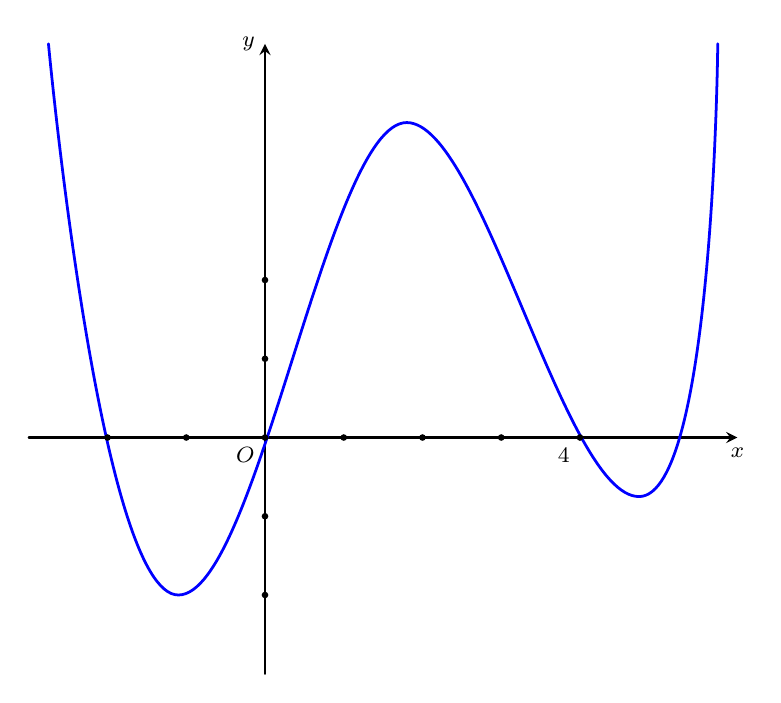
\begin{tikzpicture}[line join=round, line cap=round, >=stealth, scale=1, thick, font=\footnotesize]
			\draw[->] (-3,0)--(6,0)node[below]{$x$};
			\draw[->] (0,-3)--(0,5)node[left]{$y$};
			\draw [line width=1pt,blue ]
			(-2.75,5) .. controls + (0:.0) and + (-180:1) ..
			(-1.1,-2) .. controls + (0:1) and + (-180:1) ..
			(1.8,4) .. controls + (0:.95) and + (-180:.95) ..
			(4.75,-0.75) .. controls + (0:.95) and + (-180:.0) ..
			(5.75,5) ;
			\path
			(4,0) node[below left]{$4$}
			(0,0) node[below left]{$O$} ;
			\foreach \diemx/\diemy in {-2/0,-1/0,0/0,1/0,2/0,3/0,4/0, 0/-2,0/-1,0/1,0/2}
			\fill (\diemx,\diemy)circle(1.2pt);
		\end{tikzpicture}
	\end{center}
	\choice
	{$5$}
	{$3$}
	{\True $7$}
	{$11$}
	\loigiai{
	Từ đồ thị ta có bảng biến thiên của hàm số $y=f(x)$ như sau:
	\begin{center}
		
\begin{tikzpicture}[line cap=round, line join=round, font=\footnotesize, scale=1, thick, >=stealth]
			\tkzTabInit[nocadre,lgt=1.2,espcl=2.5]
			{$x$/0.8,$f'(x)$/0.8,$f(x)$/2.5}
			{$-\infty$,$a$,$b$,$c$,$+\infty$}
			\tkzTabLine{,-,0,+,0,-,0,+}
			\tkzTabVar{+/$+\infty$,-/$ $,+/$ $,-/$ $,+/$+\infty$}
		\end{tikzpicture}
	\end{center}
	Ta có $g(x)=f\left(x^3+3x^2\right)$ $\Rightarrow g'(x)=\left(3x^2+6x\right).f'\left(x^3+3x^2\right)$.\\
	Cho $g'(x)=0$ $\Leftrightarrow \left[\begin{aligned}
		&3x^2+6x=0\\
		&{f}'\left(x^3+3x^2\right)=0\\
	\end{aligned}\right.$ $\Leftrightarrow \left[\begin{aligned}
		&x=0\\
		&x=-2\\
		&{x^3}+3x^2=a;a<0\\
		&{x^3}+3x^2=b;0<b<4\\
		&{x^3}+3x^2=c;c>4\\
	\end{aligned}\right.$.\\
	Xét hàm số $h(x)=x^3+3x^2\Rightarrow h'(x)=3x^2+6x$. Cho $h'(x)=0$ $\Leftrightarrow \left[\begin{aligned}
		&x=0\\
		&x=-2\\
	\end{aligned}\right.$.\\
	Bảng biến thiên:
	\begin{center}
		
\begin{tikzpicture}[line cap=round, line join=round, font=\footnotesize, scale=1, thick, >=stealth]
			\tkzTabInit[nocadre,lgt=1.2,espcl=2.5]
			{$x$/0.8,$h'(x)$/0.8,$h(x)$/2.5}
			{$-\infty$,$-2$,$0$,$+\infty$}
			\tkzTabLine{,+,0,-,0,+}
			\tkzTabVar{-/$-\infty$,+/$4$,-/$0$,+/$+\infty$}
		\end{tikzpicture}
	\end{center}
	\immini{
		Ta có đồ thị của hàm $h(x)=x^3+3x^2$ như sau:\\
		Từ đồ thị ta thấy:\\
		Đường thẳng $y=a$ cắt đồ thị hàm số $y=h(x)$ tại $1$ điểm.\\
		Đường thẳng $y=b$ cắt đồ thị hàm số $y=h(x)$ tại $3$ điểm.\\
		Đường thẳng $y=c$ cắt đồ thị hàm số $y=h(x)$ tại $1$ điểm.\\
		Như vậy phương trình $g'(x)=0$ có tất cả $7$ nghiệm đơn phân biệt.\\
		Vậy hàm số $g(x)=f\left(x^3+3x^2\right)$ có $7$ cực trị.
	}{
		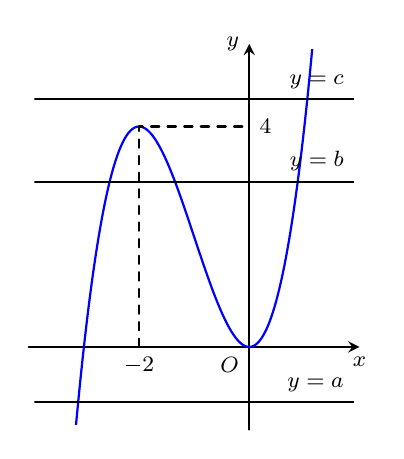
\begin{tikzpicture}[scale=.7,>=stealth, font=\footnotesize, line join=round, line cap=round, thick]
			\def\a{1} \def\b{3} \def\c{0} \def\d{0} % Hệ số
			\def\xmin{-4} \def\xmax{2}
			\def\ymin{-1.5} \def\ymax{5.5}
			%\draw[color=gray!50,dashed] (\xmin,\ymin) grid (\xmax,\ymax);
			\draw[->] (\xmin,0)--(\xmax,0) node [below]{$x$};
			\draw[->] (0,\ymin)--(0,\ymax) node [left]{$y$};
			\node at (0,0) [below left]{$O$};
			\clip (\xmin+0.1,\ymin+0.1) rectangle (\xmax-0.1,\ymax-0.1);
			\draw[smooth,samples=300,blue] plot(\x,{\a*(\x)^3+\b*(\x)^2+\c*(\x)+\d});
			\draw[dashed] (-2,0) node[below]{$-2$}--(-2,4)--(0,4) node[right]{$4$};
			\draw (-3.9,-1)--(1.9,-1) node[above left]{$y=a$}
			(-3.9,3)--(1.9,3) node[above left]{$y=b$}
			(-3.9,4.5)--(1.9,4.5) node[above left]{$y=c$}
			;
		\end{tikzpicture}
	}
}
\end{ex}
\begin{ex}[Mã 101-2019]%Câu 36%[2D1G2-2]
	Cho hàm số $y=f(x)$, bảng biến thiên của hàm số $f'(x)$ như sau:
	\begin{center}
		\begin{tikzpicture}[line cap=round, line join=round, font=\footnotesize, scale=1, thick, >=stealth]
			\tkzTabInit[nocadre,lgt=1.2,espcl=2.5]
			{$x$/0.8,$f'(x)$/2.5}
			{$-\infty$,$-1$,$0$,$1$,$+\infty$}
			%\tkzTabLine{,-,0,+,0,-,0,+}
			\tkzTabVar{%+/$+\infty$,-/$-3$,+/$2$,-/$-1$,+/$+\infty$
			}
			\path (N11) node[below](A){$+\infty$}
			(N22) node[above](B){$-3$}
			(N31) node[below](C){$2$}
			($(N42)+(0,.4)$) node[above](D){$-1$}
			(N51) node[below](E){$+\infty$}
			;
			\draw[->] (A)--(B);
			\draw[->] (B)--(C);
			\draw[->] (C)--(D);
			\draw[->] (D)--(E);
		\end{tikzpicture}
	\end{center}
	Số điểm cực trị của hàm số $y=f\left(x^2-2x\right)$ là
	\choice
	{$9$}
	{$3$}
	{\True $7$}
	{$5$}
	\loigiai{
	Ta có $y'=2\left(x-1\right).f'\left(x^2-2x\right)$.\\
	$y'=0\Leftrightarrow\left[\begin{aligned}
		&x=1\\
		&f'\left(x^2-2x\right)=0\\
	\end{aligned}\right.\Leftrightarrow\left[\begin{aligned}
		&x=1\\
		&x^2-2x=a\in\left(-\infty;-1\right)\\
		&x^2-2x=b\in\left(-1;0\right)\\
		&x^2-2x=c\in\left(0;1\right)\\
		&x^2-2x=d\in\left(1;+\infty\right)\\
	\end{aligned}\right.\Leftrightarrow\left[\begin{aligned}
		&x=1\\
		&x^2-2x-a=0,a\in\left(-\infty;-1\right)(1)\\
		&x^2-2x-b=0,b\in\left(-1;0\right)(2)\\
		&x^2-2x-c=0,c\in\left(0;1\right)(3)\\
		&x^2-2x-d=0,d\in\left(1;+\infty\right)(4)\\
	\end{aligned}\right.$.\\
	Phương trình $(1)$ vô nghiệm, các phương trình $(2)$, $(3)$, $(4)$ đều có hai nghiệm phân biệt khác $1$ và do $b$, $c$, $d$ đôi một khác nhau nên các nghiệm của phương trình $(2)$, $(3)$, $(4)$ cũng đôi một khác nhau. Do đó $f'\left(x^2-2x\right)=0$ có 6 nghiệm phân biệt.\\
	Vậy $y'=0$ có $7$ nghiệm phân biệt, do đó số điểm cực trị của hàm số $y=f\left(x^2-2x\right)$ là $7$.
}
\end{ex}
\begin{ex}[Mã 104-2019]%Câu 37%[2D1G2-2]
	Cho hàm số $f(x)$, bảng biến thiên của hàm số $f'(x)$ như sau:
	\begin{center}
		\begin{tikzpicture}[line cap=round, line join=round, font=\footnotesize, scale=1, thick, >=stealth]
			\tkzTabInit[nocadre,lgt=1.2,espcl=2.5]
			{$x$/0.8,$f'(x)$/2.5}
			{$-\infty$,$-1$,$0$,$1$,$+\infty$}
			%\tkzTabLine{,-,0,+,0,-,0,+}
			\tkzTabVar{%+/$+\infty$,-/$-3$,+/$2$,-/$-1$,+/$+\infty$
			}
			\path (N11) node[below](A){$+\infty$}
			(N22) node[above](B){$-3$}
			(N31) node[below](C){$2$}
			($(N42)+(0,.4)$) node[above](D){$-1$}
			(N51) node[below](E){$+\infty$}
			;
			\draw[->] (A)--(B);
			\draw[->] (B)--(C);
			\draw[->] (C)--(D);
			\draw[->] (D)--(E);
		\end{tikzpicture}
	\end{center}
	Số điểm cực trị của hàm số $y=f\left(4x^2+4x\right)$ là
	\choice
	{$5$}
	{$9$}
	{\True $7$}
	{$3$}
	\loigiai{
	Có $\left(f\left(4x^2+4x\right)\right)'=\left(8x+4\right){f}'\left(4x^2+4x\right)$, $\left(f\left(4x^2+4x\right)\right)'=0\Leftrightarrow\left[\begin{aligned}
		&x=-\dfrac{1}{2}\\
		&{f}'\left(4x^2+4x\right)=0\\
	\end{aligned}\right.$.
	\begin{center}
		\begin{tikzpicture}[line cap=round, line join=round, font=\footnotesize, scale=1, thick, >=stealth]
			\tkzTabInit[nocadre,lgt=1.2,espcl=2.5]
			{$x$/0.8,$f'(x)$/2.5}
			{$-\infty$,$-1$,$0$,$1$,$+\infty$}
			%\tkzTabLine{,-,0,+,0,-,0,+}
			\tkzTabVar{%+/$+\infty$,-/$-3$,+/$2$,-/$-1$,+/$+\infty$
			}
			\path (N11) node[below](A){$+\infty$}
			(N22) node[above](B){$-3$}
			(N31) node[below](C){$2$}
			($(N42)+(0,.4)$) node[above](D){$-1$}
			(N51) node[below](E){$+\infty$}
			($(N11)!.5!(N22)$) node[above]{$a_1$}
			($(N22)!.5!(N31)$) node[above]{$a_2$}
			($(N31)!.5!(N42)$) node[above right]{$a_3$}
			($(N42)!.5!(N51)$) node[above left]{$a_4$}
			;
			\draw[->] (A)--(B);
			\draw[->] (B)--(C);
			\draw[->] (C)--(D);
			\draw[->] (D)--(E);
			\draw ($(N11)!.5!(N12)$)--($(N51)!.5!(N52)$);
		\end{tikzpicture}
	\end{center}
	Từ bảng biến thiên trên ta có $f'\left(4x^2+4x\right)=0\Leftrightarrow\left[\begin{aligned}
		&4x^2+4x=a_1\in\left(-\infty;-1\right)\\
		&4x^2+4x=a_2\in\left(-1;0\right)\\
		&4x^2+4x=a_3\in\left(0;1\right)\\
		&4x^2+4x=a_4\in\left(1;+\infty\right)\\
	\end{aligned}\right.$ $(1)$.\\
	Xét $g(x)=4x^2+4x$, $g'(x)=8x+4$, $g'(x)=0\Leftrightarrow x=-\dfrac{1}{2}$ ta có bảng biến thiên
	\begin{center}
		
\begin{tikzpicture}[line cap=round, line join=round, font=\footnotesize, scale=1, thick, >=stealth]
			\tkzTabInit[nocadre,lgt=1.5,espcl=2.5]
			{$x$/0.9,$g'(x)$/0.8,$g(x)$/2.5}
			{$-\infty$,$-\dfrac{1}{2}$,$+\infty$}
			\tkzTabLine{,-,0,+,}
			\tkzTabVar{+/$+\infty$,-/$-1$,+/$+\infty$}
		\end{tikzpicture}
	\end{center}
	Kết hợp bảng biến thiên của $g(x)$ và hệ $(1)$ ta thấy:\\
	Phương trình $4x^2+4x=a_1\in\left(-\infty;-1\right)$ vô nghiệm.\\
	Phương trình $4x^2+4x=a_2\in\left(-1;0\right)$ tìm được hai nghiệm phân biệt khác $-\dfrac{1}{2}$.\\
	Phương trình $4x^2+4x=a_2\in\left(0;1\right)$ tìm được thêm hai nghiệm mới phân biệt khác $-\dfrac{1}{2}$.\\
	Phương trình $4x^2+4x=a_2\in\left(1;+\infty\right)$ tìm được thêm hai nghiệm phân biệt khác $-\dfrac{1}{2}$.\\
	Vậy hàm số $y=f\left(4x^2+4x\right)$ có tất cả $7$ điểm cực trị.
	}
\end{ex}
\begin{ex}[Chuyên ĐH Vinh-Nghệ An-2020]%Câu 38%[2D1G2-2]
	Cho hàm số $f(x)$ có đạo hàm liên tục trên $\mathbb{R}$. Đồ thị hàm số $y=f'(x)$ như hình vẽ bên. Hàm số $y=f\left(x^2+4x\right)-x^2-4x$ có bao nhiêu điểm cực trị thuộc khoảng $\left(-5;1\right)$ ?
	\begin{center}
		\begin{tikzpicture}[scale=.7,>=stealth, font=\footnotesize, line join=round, line cap=round, thick]
			\def\a{1} \def\b{-4} \def\c{3} % Hệ số
			\def\xmin{-6} \def\xmax{6}
			\def\ymin{-3} \def\ymax{4.5}
			%\draw[color=gray!50,dashed] (\xmin,\ymin) grid (\xmax,\ymax);
			\draw[->] (\xmin,0)--(\xmax,0) node [below]{$x$};
			\draw[->] (0,\ymin)--(0,\ymax) node [left]{$y$};
			\node at (0,0) [below left]{$O$};
			\clip (\xmin+0.1,\ymin+0.1) rectangle (\xmax-0.1,\ymax-0.1);
			\draw[smooth,samples=300]
			plot[domain=-5.5:-4](\x,{-2*(\x+4)^2+1})
			plot[domain=-4:1](\x,{.5*(\x)^2+2*(\x)+1})
			plot[domain=1:5.5](\x,{-1/3*(\x-1)^2+3.5}) ;
			\draw[dashed] (-5,0) node[below left]{$-5$}--(-5,-1)
			(-4,0) node[below]{$-4$}--(-4,1)--(0,1) node[right]{$1$}
			(1,0) node[below]{$1$}--(1,3.5)
			(5,0) node[below left]{$5$}--(5,-1.83) ;
		\end{tikzpicture}
	\end{center}
	\choice
	{\True $5$}
	{$4$}
	{$6$}
	{$3$}
	\loigiai{
	Đặt $g(x)=f\left(x^2+4x\right)-x^2-4x$.\\
	$\Rightarrow{g}'(x)=\left(2x+4\right){f}'\left(x^2+4x\right)-\left(2x+4\right)=\left(2x+4\right)\left[f'\left(x^2+4x\right)-1\right]$.\\
	Ta có $g'(x)=0\Leftrightarrow\left[\begin{aligned}
		&2x+4=0\\
		&{x^2}+4x=-4~(1)\\
		&{x^2}+4x=0~(2)\\
		&{x^2}+4x=a\in\left(1;5\right)(3)\\
	\end{aligned}\right.$.\\
	Xét phương trình $x^2+4x=a\in\left(1;5\right)$, ta có bảng biến thiên của hàm số $y=x^2+4x$ trên $\left(-5;1\right)$ như sau:
	\begin{center}
		\begin{tikzpicture}[line cap=round, line join=round, font=\footnotesize, scale=1, thick, >=stealth]
			\tkzTabInit[nocadre,lgt=1,espcl=2.5]
			{$x$/0.8,$y'$/0.8,$y$/2.5}
			{$-5$,$-4$,$-2$,$0$,$1$}
			\tkzTabLine{,,-,,0,,+,,}
			\tkzTabVar{%+/$5$,R,-/$-4$,R,+/$5$
			}
			\path (N12) node[below](A){$5$}
			($(N12)!.5!(N33)$) node(B){$0$}
			(N33) node[above](C){$-4$}
			($(N33)!.5!(N52)$) node(D){$0$}
			(N52) node[below](E){$5$}
			;
			\draw[->] (A)--(B); \draw[->] (B)--(C); \draw[->] (C)--(D); \draw[->] (D)--(E);
		\end{tikzpicture}
	\end{center}
	Suy ra $(1)$ có nghiệm kép $x=-2$, $(2)$ có $2$ nghiệm phân biệt $x=-4$; $x=0$, $(3)$ có $2$ nghiệm phân biệt $x=x_1$; $x=x_2$ khác $-2$; $0$; $-4$. Do đó phương trình $g'(x)=0$ có $5$ nghiệm trong đó có $x=-2$ là nghiệm bội ba, các nghiệm $x=-4$; $x=0$; $x=x_1$; $x=x_2$ là các nghiệm đơn.\\
	Vậy $g(x)$ có $5$ điểm cực trị.
}
\end{ex}
\begin{ex}[Chuyên Hưng Yên-2020]%Câu 39%[2D1G2-2]
	Cho hàm số $y=f(x)$ có đạo hàm đến cấp hai trên $\mathbb{R}$ và có bảng xét dấu của hàm số $y=f'(x)$ như hình sau:
	\begin{center}
		\begin{tikzpicture}
			\tkzTabInit[nocadre,lgt=1.5,espcl=2,deltacl=0.6]
			{$x$ /0.6,$f'(x)$ /0.6}
			{$-\infty$,$-2$,$0$,$4$,$+\infty$}
			\tkzTabLine{,-,$0$,+,$0$,-,$0$,+,}
		\end{tikzpicture}
	\end{center}
	Hỏi hàm số $g(x)=f\left(1-x\right)+\dfrac{x^3}{3}-2x^2+3x$ đạt cực tiểu tại điểm nào trong các điểm sau?
	\choice
	{\True $x=3$}
	{$x=0$}
	{$x=-3$}
	{$x=1$}
	\loigiai{
	$g'(x)=-f'\left(1-x\right)+x^2-4x+3$.\\
	$-f'\left(1-x\right)>0\Leftrightarrow{f}'\left(1-x\right)<0\Leftrightarrow\left[\begin{aligned}
		&1-x<-2\\
		&0<1-x<4\\
	\end{aligned}\right.\Leftrightarrow\left[\begin{aligned}
		&x>3\\
		&-3<x<1\\
	\end{aligned}\right.$.\\
	Bảng xét dấu $g'(x)$:
	\begin{center}
		\begin{tikzpicture}
			\tkzTabInit[nocadre,lgt=2.5,espcl=2.85,deltacl=0.6]
			{$x$ /0.6,$-f'(1-x)$ /0.6,$x^2-4x+3$/0.6,$g'(x)$/0.6}
			{$-\infty$,$-3$,$1$,$3$,$+\infty$}
			\tkzTabLine{,-,$0$,+,$0$,-,$0$,+,}
			\tkzTabLine{,+,d,+,$0$,-,$0$,+,}
			\tkzTabLine{,\text{không xác định},d,+,$0$,-,$0$,+,}
		\end{tikzpicture}
	\end{center}
	Từ bảng xét dấu $g'(x)$ ta suy ra hàm số đạt cực tiểu tại $x=3$.
}
\end{ex}
\begin{ex}[Chuyên KHTN-2020]%Câu 40%[2D1G2-2]
	Cho hàm số $y=f(x)$ xác định trên $\mathbb{R}$, có đồ thị $f(x)$ như hình vẽ.
	\begin{center}
		\begin{tikzpicture}[scale=1,>=stealth, font=\footnotesize, line join=round, line cap=round, thick]
			\def\a{-1} \def\b{3} \def\c{0} \def\d{-1} % Hệ số
			\def\xmin{-2} \def\xmax{4}
			\def\ymin{-2} \def\ymax{4}
			%\draw[color=gray!50,dashed] (\xmin,\ymin) grid (\xmax,\ymax);
			\draw[->] (\xmin,0)--(\xmax,0) node [below]{$x$};
			\draw[->] (0,\ymin)--(0,\ymax) node [left]{$y$};
			\node at (0,0) [below left]{$O$};
			\clip (\xmin+0.1,\ymin+0.1) rectangle (\xmax-0.1,\ymax-0.1);
			\draw[smooth,samples=300] plot(\x,{\a*(\x)^3+\b*(\x)^2+\c*(\x)+\d});
			\draw[dashed] (0,-1) node[below right]{$-1$}
			(2,0) node[below]{$2$}--(2,3)--(0,3) node[left]{$3$}
			(3,-1) node[above,rotate=-84]{$y=f(x)$};
		\end{tikzpicture}
	\end{center}
	Hàm số $g(x)=f\left(x^3+x\right)$ đạt cực tiểu tại điểm $x_0$. Giá trị $x_0$ thuộc khoảng nào sau đây
	\choice
	{$\left(1;3\right)$}
	{\True $\left(-1;1\right)$}
	{$\left(0;2\right)$}
	{$\left(3;+\infty\right)$}
	\loigiai{
	Ta có $g(x)=f\left(x^3+x\right)\Rightarrow{g}'(x)=\left(3x^2+1\right){f}'\left(x^3+x\right)$.\\
	$\Rightarrow{g}'(x)=0\Leftrightarrow\left(3x^2+1\right){f}'\left(x^3+x\right)=0\Leftrightarrow{f}'\left(x^3+x\right)=0\Leftrightarrow\left[\begin{aligned}
		&x^3+x=0\\
		&x^3+x=2\\
	\end{aligned}\right.\Leftrightarrow\left[\begin{aligned}
		&x=0\\
		&x=1\\
	\end{aligned}\right.$.\\
	Do đó $g'(x)>0\Leftrightarrow\left(3x^2+1\right){f}'\left(x^3+x\right)>0\Leftrightarrow{f}'\left(x^3+x\right)>0\Leftrightarrow 0<x^3+x<2\Leftrightarrow 0<x<1$.\\
	Bảng biến thiên:
	\begin{center}
		\begin{tikzpicture}
			\tkzTabInit[nocadre,lgt=1.2,espcl=2.5,deltacl=0.6]
			{$x$ /0.6, $g'(x)$ /0.6, $g(x)$ /2.5}
			{$-\infty$,$0$,$1$,$+\infty$}
			\tkzTabLine{,-,$0$,+,$0$,-,}
			\tkzTabVar{+/$+\infty$,-/$ $,+/$ $,-/$-\infty$}
		\end{tikzpicture}
	\end{center}
	Vây hàm số $g(x)=f\left(x^3+x\right)$ đạt cực tiểu tại điểm $x_0=0$. Suy ra $x_0\in\left(-1;1\right)$.
}
\end{ex}
\begin{ex}[Chuyên KHTN-2020]%Câu 41%[2D1G2-2]
	Cho hàm số $y=f(x)$ liên tục trên $\mathbb{R}$, có đồ thị $f'(x)$ như hình vẽ.
	\begin{center}
		\begin{tikzpicture}[scale=1,>=stealth, font=\footnotesize, line join=round, line cap=round, thick]
			\def\a{0} \def\b{1} \def\c{-2} \def\d{0} % Hệ số
			\def\xmin{-1.5} \def\xmax{3.5}
			\def\ymin{-1.5} \def\ymax{3.5}
			%\draw[color=gray!50,dashed] (\xmin,\ymin) grid (\xmax,\ymax);
			\draw[->] (\xmin,0)--(\xmax,0) node [below]{$x$};
			\draw[->] (0,\ymin)--(0,\ymax) node [left]{$y$};
			\node at (0,0) [below left]{$O$};
			\clip (\xmin+0.1,\ymin+0.1) rectangle (\xmax-0.1,\ymax-0.1);
			\draw[smooth,samples=300] plot(\x,{\a*(\x)^3+\b*(\x)^2+\c*(\x)+\d});
			\draw[dashed] (2,0) node[below]{$2$}
			(2.7,2) node[above,rotate=72]{$y=f(x)$};
		\end{tikzpicture}
	\end{center}
	Số điểm cực tiểu của hàm số $g(x)=f\left(-x^2+x\right)$ là
	\choice
	{\True $1$}
	{$4$}
	{$3$}
	{$2$}
	\loigiai{
	Ta có $g(x)=f\left(-x^2+x\right)\Rightarrow{g}'(x)=\left(-2x+1\right){f}'\left(-x^2+x\right)$.\\
	$\Rightarrow{g}'(x)=0\Leftrightarrow\left(-2x+1\right){f}'\left(-x^2+x\right)=0\Leftrightarrow\left[\begin{aligned}
		&-2x+1=0\\
		&f'\left(-x^2+x\right)=0\\
	\end{aligned}\right.\Leftrightarrow\left[\begin{aligned}
		&x=\dfrac{1}{2}\\
		&-x^2+x=0\\
		&-x^2+x=2\\
	\end{aligned}\right.\Leftrightarrow\left[\begin{aligned}
		&x=\dfrac{1}{2}\\
		&x=1\\
		&x=0\\
	\end{aligned}\right.$.\\
	Do đó $g'(x)>0\Leftrightarrow\left(-2x+1\right){f}'\left(-x^2+x\right)>0\Leftrightarrow\left[\begin{aligned}
		&\left\{\begin{aligned}
			&-2x+1>0\\
			&f'\left(-x^2+x\right)>0\\
		\end{aligned}\right.\\
		&\left\{\begin{aligned}
			&-2x+1<0\\
			&f'\left(-x^2+x\right)<0\\
		\end{aligned}\right.\\
	\end{aligned}\right.$.\\
	$\Leftrightarrow\left[\begin{aligned}
		&\left\{\begin{aligned}
			&x<\dfrac{1}{2}\\
			&\left[\begin{aligned}
				&-x^2+x>2\\
				&-x^2+x<0\\
			\end{aligned}\right.\\
		\end{aligned}\right.\\
		&\left\{\begin{aligned}
			&x>\dfrac{1}{2}\\
			&0<-x^2+x<2\\
		\end{aligned}\right.\\
	\end{aligned}\right.\Leftrightarrow\left[\begin{aligned}
		&\left\{\begin{aligned}
			&x<\dfrac{1}{2}\\
			&\left[\begin{aligned}
				&x>1\\
				&x<0\\
			\end{aligned}\right.\\
		\end{aligned}\right.\\
		&\left\{\begin{aligned}
			&x>\dfrac{1}{2}\\
			&0<x<1\\
		\end{aligned}\right.\\
	\end{aligned}\right.\Leftrightarrow\left[\begin{aligned}
		&x<0\\
		&\dfrac{1}{2}<x<1\\
	\end{aligned}\right.$.\\
	Bảng biến thiên
	\begin{center}
		\begin{tikzpicture}
			\tkzTabInit[nocadre,lgt=1.2,espcl=2.5,deltacl=0.6]
			{$x$ /1, $g'(x)$ /0.8, $g(x)$ /2}
			{$-\infty$,$0$,$\dfrac{1}{2}$,$1$,$+\infty$}
			\tkzTabLine{,+,$0$,-,$0$,+,$0$,-,}
			\tkzTabVar{-/$-\infty$,+/$ $,-/$ $,+/$ $,-/$-\infty$}
		\end{tikzpicture}
	\end{center}
	Vậy hàm số có $1$ điểm cực tiểu.
}
\end{ex}
\begin{ex}[Chuyên Lam Sơn-2020]%Câu 42%[2D1G2-2]
Cho hàm số $y=f(x)$ có đạo hàm liên tục trên $\mathbb{R}$, bảng biến thiên của hàm số $f'(x)$ như sau:
\begin{center}
	\begin{tikzpicture}
		\tkzTabInit[nocadre,lgt=1.2,espcl=2.5]
		{$x$/0.8,$f'(x)$/2.5}
		{$-\infty$,$-1$,$1$,$+\infty$}
		%\tkzTabLine{,+,0,-,0,+}
		\tkzTabVar{-/$-\infty$,+/$4$,-/$-2$,+/$+\infty$}
	\end{tikzpicture}
\end{center}
	Số điểm cực trị của hàm số $y=f\left(x^2+2x\right)$ là
	\choice
	{$4$}
	{\True $5$}
	{$1$}
	{$7$}
	\loigiai{
	Ta có $y'=\left(2x+2\right)f'\left(x^2+2x\right)=0\Leftrightarrow\left[\begin{aligned}
		&x=-1\\
		&f'\left(x^2+2x\right)=0~(1)\\
	\end{aligned}\right.$.\\
	Từ bảng biến thiên ta thấy phương trình $(1)\Leftrightarrow\left[\begin{aligned}
		&x^2+2x=a<-1~(2)\\
		&x^2+2x=b\in\left(-1;1\right)~(3)\\
		&x^2+2x=c>1~(4)\\
	\end{aligned}\right.$.\\
	Đồ thị hàm số $y=x^2+2x$ có dạng:
	\begin{center}
		\begin{tikzpicture}[scale=1,>=stealth, font=\footnotesize, line join=round, line cap=round, thick]
			\def\a{0} \def\b{1} \def\c{2} \def\d{0} % Hệ số
			\def\xmin{-3.5} \def\xmax{1.5}
			\def\ymin{-1.5} \def\ymax{3.5}
			%\draw[color=gray!50,dashed] (\xmin,\ymin) grid (\xmax,\ymax);
			\draw[->] (\xmin,0)--(\xmax,0) node [below]{$x$};
			\draw[->] (0,\ymin)--(0,\ymax) node [left]{$y$};
			\node at (0,0) [below right]{$O$};
			\clip (\xmin+0.1,\ymin+0.1) rectangle (\xmax-0.1,\ymax-0.1);
			\draw[smooth,samples=300] plot(\x,{\a*(\x)^3+\b*(\x)^2+\c*(\x)+\d});
			\draw[dashed] (-2,0) node[below left]{$-2$};
		\end{tikzpicture}
	\end{center}
	Từ đồ thị hàm số $y=x^2+2x$ ta thấy phương trình $(2)$ vô nghiệm; phương trình $(3)$; phương trình $(4)$ đều có $2$ nghiệm phân biệt.\\
	Do đó $y'=0$ có $5$ nghiệm đơn phân biệt. Vậy hàm số $y=f\left(x^2+2x\right)$ có $5$ điểm cực trị.
}
\end{ex}
\begin{ex}[Sở Bắc Giang-2018]%Câu 43%[2D1G2-1]
	Cho hàm số $y=f(x)$ có đúng ba điểm cực trị là $-2$; $-1$; $0$ và có đạo hàm liên tục trên $\mathbb{R}$. Khi đó hàm số $y=f\left(x^2-2x\right)$ có bao nhiêu điểm cực trị?
	\choice
	{\True $3$}
	{$8$}
	{$10$}
	{$7$}
	\loigiai{
	Vì hàm số $y=f(x)$ có đúng ba điểm cực trị là $-2$; $-1$; $0$ và có đạo hàm liên tục trên $\mathbb{R}$ nên $f'(x)=0$ có ba nghiệm là $-2$; $-1$; $0$ (ba nghiệm bội lẻ).\\
	Xét hàm số $y=f\left(x^2-2x\right)$ có $y'=\left(2x-2\right).f'\left(x^2-2x\right)$; $y'=0\Leftrightarrow\left(2x-2\right).f'\left(x^2-2x\right)=0$.\\
	$\Leftrightarrow\left[\begin{aligned}
		&x=1\\
		&x^2-2x=-2\\
		&x^2-2x=-1\\
		&x^2-2x=0\\
	\end{aligned}\right.\Leftrightarrow\left[\begin{aligned}
		&x=1\\
		&x=0\\
		&x=2\\
	\end{aligned}\right.$.\\
	Do $y'=0$ có một nghiệm bội lẻ ($x=1$) và hai nghiệm đơn ($x=0$; $x=2$) nên hàm số $y=f\left(x^2-2x\right)$ chỉ có ba điểm cực trị.
}
\end{ex}
\begin{ex}[Mã 102-2019]%Câu 44%[2D1G2-2]
	Cho hàm số $f(x)$, bảng biến thiên của hàm số $f'(x)$ như sau
	\begin{center}
		\begin{tikzpicture}[line cap=round, line join=round, font=\footnotesize, scale=1, thick, >=stealth]
			\tkzTabInit[nocadre,lgt=1.2,espcl=2.5]
			{$x$/0.8,$f'(x)$/2.5}
			{$-\infty$,$-1$,$0$,$1$,$+\infty$}
			%\tkzTabLine{,-,0,+,0,-,0,+}
			\tkzTabVar{%+/$+\infty$,-/$-3$,+/$2$,-/$-1$,+/$+\infty$
			}
			\path (N11) node[below](A){$+\infty$}
			(N22) node[above](B){$-3$}
			(N31) node[below](C){$2$}
			($(N42)+(0,.4)$) node[above](D){$-1$}
			(N51) node[below](E){$+\infty$}
			;
			\draw[->] (A)--(B); \draw[->] (B)--(C);
			\draw[->] (C)--(D);\draw[->] (D)--(E);
		\end{tikzpicture}
	\end{center}
	Số điểm cực trị của hàm số $y=f\left(x^2+2x\right)$ là
	\choice
	{$9$}
	{$5$}
	{\True $7$}
	{$3$}
	\loigiai{
	Ta có $y'=\left(2x+2\right)f'\left(x^2+2x\right)=0\Leftrightarrow\left[\begin{aligned}
		&2x+2=0\\
		&x^2+2x=a,a<-1\\
		&x^2+2x=b,-1<b<0\\
		&x^2+2x=c,0<c<1\\
		&x^2+2x=d,d>1\\
	\end{aligned}\right.$.
	\begin{center}
		\begin{tikzpicture}[scale=1,>=stealth, font=\footnotesize, line join=round, line cap=round, thick]
			\def\a{0} \def\b{1} \def\c{2} \def\d{0} % Hệ số
			\def\xmin{-3.5} \def\xmax{1.5}
			\def\ymin{-2} \def\ymax{3.5}
			%\draw[color=gray!50,dashed] (\xmin,\ymin) grid (\xmax,\ymax);
			\draw[->] (\xmin,0)--(\xmax,0) node [below]{$x$};
			\draw[->] (0,\ymin)--(0,\ymax) node [left]{$y$};
			\node at (0,0) [below right]{$O$};
			\clip (\xmin+0.1,\ymin+0.1) rectangle (\xmax-0.1,\ymax-0.1);
			\draw[smooth,samples=300,magenta] plot(\x,{\a*(\x)^3+\b*(\x)^2+\c*(\x)+\d});
			\path[fill=black] (-2,0) node[below left]{$-2$}
			(0,-1) circle(1pt) node[right]{$-1$}
			(0,1) circle(1pt) node[right]{$1$}
			(0,2) circle(1pt) node[right]{$2$};
			\draw[blue] (-3.3,-1.5)--(1.3,-1.5) node[above left]{$a$}
			(-3.3,-.5)--(1.3,-.5) node[above left]{$b$}
			(-3.3,.5)--(1.3,.5) node[above left]{$c$}
			(-3.3,1.5)--(1.3,1.5) node[above left]{$d$}
			;
		\end{tikzpicture}
	\end{center}
	Dựa vào đồ thị ta được $y'=0$ có $7$ nghiệm đơn nên nó có $7$ cực trị.
	}
\end{ex}
\begin{ex}%[2D1K2-2][Mã 103-2019]%Câu 45
	Cho hàm số $f(x)$, bảng biến thiên của hàm số $f'(x)$ như sau:
	\begin{center}
		\begin{tikzpicture}
			\tkzTabInit[lgt=1.2,espcl=3]
			{$x$/1.2,$f'(x)$/2.5}
			{$-\infty$,$-1$,$0$,$1$,$+\infty$}
			%\tkzTabLine{ ,-,z,+,z,-,z,+, }
			\tkzTabVar{+/$+\infty$,-/$-3$,+/$2$,-/$-1$,+/$+\infty$}
		\end{tikzpicture}
	\end{center}
	\noindent 
	Số cực trị của hàm số $y=f\left(4x^2-4x\right)$ là
	\choice
	{$3$}
	{$9$}
	{$5$}
	{\True $7$}
	\loigiai{
		Từ bảng biến thiên 
		\begin{center}
			\begin{tikzpicture}
				\tkzTabInit[lgt=1.2,espcl=3]
				{$x$/0.6,$ f''(x) $/0.6,$f'(x)$/3.0}
				{$-\infty$,$-1$,$0$,$1$,$+\infty$}
				\tkzTabLine{ ,-,z,+,z,-,z,+, }
				%\tkzTabVar{+/$+\infty$,-/$f(x_1)$,+/$c$,-/$f(x_2)$,+/$+\infty$}
				\path
				(N12)node[below](1){$+\infty$}
				(N23)node[above](2){$ -3 $}
				(N32)node[below](3){$ 2 $}
				(N43)node[above](4){$ -1 $}
				(N52)node[below](5){$ +\infty $}
				(M11)node[above](6){$ a $}
				(M21)node[above](7){$ b$}
				(M31)node[above](8){$ c $}
				(M41)node[above](9){$ d $}
				($ (M12)!0.5!(M13) $) node(10){}
				($ (M22)!0.5!(M23) $) node(11){}
				($ (M32)!0.5!(M33) $) node(12){}
				($ (M42)!0.5!(M43) $) node(13){}
				;
				\foreach \x/\y in {1/10,10/2,2/11,11/3,3/12,12/4,4/13,13/5}\draw[-stealth] (\x)--(\y);
				\draw ($ (N12)!0.5!(N13) $) --($ (N52)!0.5!(N53) $);
				\draw[dashed] (6)--(10) (7)--(11) (8)--(12) (9)--(13);
			\end{tikzpicture}
		\end{center}
		\noindent 
		Ta thấy $f'(x)=0\Leftrightarrow \hoac{
			&x=a\in\left(-\infty;-1\right)\\
			&x=b\in\left(-1;0\right)\\
			&x=c\in\left(0;1\right)\\
			&x=d\in\left(1;+\infty\right).
		}
		$ \\
		Với $y=f\left(4x^2-4x\right)$, ta có $y'=\left(8x-4\right) f '\left(4x^2-4x\right)$.\\
		$y'=0\Leftrightarrow\hoac{
			&8x-4=0\\
			&f'\left(4x^2-4x\right)=0 
		}\Leftrightarrow\hoac{
			&x=\dfrac{1}{2}\\
			&4x^2-4x=a\in\left(-\infty ;-1\right)(1)\\
			&4x^2-4x=b\in\left(-1;0\right)(2)\\
			&	4x^2-4x=c\in\left(0;1\right)(3)\\
			&	4x^2-4x=d\in\left(1;+\infty\right)(4).
		}$\\
		Xét hàm số $g(x)=4x^2-4x$, ta có $g'(x)=8x-4=0\Leftrightarrow x=\dfrac{1}{2}$.\\
		Bảng biến thiên\\
		\begin{center}
			\begin{tikzpicture}
				\tkzTabInit[lgt=1.2,espcl=3]
				{$x$/0.8, $g’(x)$/0.8, $g(x)$/2.5}
				{$-\infty$,$\tfrac{1}{2}$, $+\infty$}
				\tkzTabLine{ ,-,z,-, }
				\tkzTabVar{+/$+\infty$,-/$-1$,+/$+\infty$}
			\end{tikzpicture}
		\end{center}
		\noindent		Từ bảng biến thiên của $g(x)$ ta có:
		\begin{itemize}
			\item Vì $a\in\left(-\infty;-1\right)$ nên $(1)$ vô nghiệm.
			\item Vì $b\in\left(-1;0\right)$ nên $(2)$ có $2$ nghiệm phân biệt.
			\item Vì $c\in\left(0;1\right)$ nên $(3)$ có $2$ nghiệm phân biệt.
			\item Vì $d\in\left(1;+\infty\right)$ nên $(4)$ có $2$ nghiệm phân biệt.
		\end{itemize}
		Vậy hàm số $y=f\left(4x^2-4x\right)$ có $7$ điểm cực trị\\
		\textbf{Cách khác:}\\
		Ta có: $y'=\left(8x-4\right)\cdot f'\left(4x^2-4x\right)$.\\
		$y'=0\Leftrightarrow\left(8x-4\right)\cdot f'\left(4x^2-4x\right)=0
		\Leftrightarrow\hoac{
			&8x-4=0\\
			&f'\left(4x^2-4x\right)=0}$\\
		\begin{itemize}
			\item $8x-4=0\Leftrightarrow x=\dfrac{1}{2}$.\\
			\item 	$f'\left(4x^2-4x\right)=0\Leftrightarrow\hoac{
				&4x^2-4x=a\left(a<-1\right)~(1)\\
				&4x^2-4x=b\left(-1<b<0\right)~(2)\\					 
				&4x^2-4x=c\left(0<c<1\right)~(3)\\
				&4x^2-4x=d\left(d>1\right).~(4)\\
			}$
		\end{itemize}
		Phương trình $4x^2-4x=m\Leftrightarrow 4x^2-4x-m=0$ có nghiệm khi $\Delta'=4-4m\ge 0$ hay $m\le 1$.\\
		Từ đó, ta có phương trình $(1)$; $(2)$; $(3)$ luôn có hai nghiệm phân biệt.\\
		Phương trình $(4)$ vô nghiệm.\\
		Do đó, hàm số đã cho có $7$ cực trị.
	}
\end{ex}
\begin{ex}%[2D1K2-2][Chuyên An Giang-2018]%Câu 46
	\immini{Cho hàm số $y=f(x)$. Đồ thị của hàm số $y=f'(x)$ như hình bên. 
		\noindent	Hàm số $g(x)=f\left(x^2\right)$ có bao nhiêu điểm cực trị?
		\choice
		{$4$}
		{$3$}
		{\True $5$}
		{$2$}}{\begin{tikzpicture}
			\draw[gray!30](-3,-5) grid (4,4);
			\draw[->] (-3,0)--(4,0)node[below]{$ x $};
			\draw[->] (0,-5)--(0,4) node[left]{$ y $};
			\draw (-2.3,-4)..controls+(80:0.5) and +(-90:0.5)..
			(-2,0)..controls +(80:0.5)and +(180:0.5)..
			(-1.5,2)..controls+(0:0.5) and+(180:0.5)..
			(0,0)..controls+(0:0.5) and+(140:0.5)..
			(1,0)..controls+(-45:0.5) and+(180:0.5)..
			(2.5,-5)..controls+(0:0.5) and +(-90:0.5)..
			(3,0)..controls +(90:0.2)and+(-90:0.5)..(3.1,2);
			\draw[fill=black] (-2,0)circle (1pt) node[shift={(120:0.5)}]{$ -2 $};
			\draw[fill=black] (1,0)circle (1pt) node[shift={(40:0.5)}]{$ 1 $};
			\draw[fill=black] (3,0)circle (1pt) node[shift={(-20:0.5)}]{$ 3 $};
			\draw[fill=black] (0,0)circle (1pt) node[shift={(-20:0.5)}]{$ O $};
			%    \foreach \p/\g in {A/90,B/90,C/-90,D/-90} \draw[fill] (\p) circle(.5pt)node [shift={(\g:.3)}] {$\p$};
	\end{tikzpicture}}
	\loigiai{
		Từ đồ thị $y=f'(x)$ ta có $f'(x)=0\Leftrightarrow\left[\begin{aligned}
			&x=-2\\ 
			&x=0\\ 
			&x=1\\ 
			&x=3. 
		\end{aligned}\right.$\\
		$f'(x)>0\Leftrightarrow\left[\begin{aligned}
			&x>3\\ 
			&-2<x<1\\ 
		\end{aligned}\right.$; $f'(x)<0\Leftrightarrow\left[\begin{aligned}
			&x<-2\\ 
			&1<x<3\\ 
		\end{aligned}\right.$.\\
		Ta có $g'(x)=2x{f}'\left(x^2\right)$; $g'(x)=0\Leftrightarrow\left[\begin{aligned}
			&x=0\\ 
			&f'\left(x^2\right)=0\\ 
		\end{aligned}\right.\Leftrightarrow\left[\begin{aligned}
			&x=0\\ 
			&x^2=1\\ 
			&x^2=3\\ 
			&x^2=0\\ 
		\end{aligned}\right.\Leftrightarrow\left[\begin{aligned}
			&x=0\\ 
			&x=\pm 1\\ 
			&x=\pm\sqrt{3}. 
		\end{aligned}\right.$ \\
		Ta có $f'\left(x^2\right)>0\Leftrightarrow\left[\begin{aligned}
			&0<x^2<1\\ 
			&x^2>3\\ 
		\end{aligned}\right.\Leftrightarrow\left[\begin{aligned}
			&\left\{\begin{aligned}
				&-1<x<1\\ 
				& x\ne 0\\ 
			\end{aligned}\right.\\ 
			&\left[\begin{aligned}
				&x>\sqrt{3}\\ 
				&x<-\sqrt{3}.
			\end{aligned}\right.\\ 
		\end{aligned}\right.$ \\
		Ta có bảng biến thiên
		
		\begin{center}
			\begin{tikzpicture}
				\tkzTabInit[lgt=1.2,espcl=2.5]
				{$x$ /0.8, $ g'(x) $ /0.8, $g(x)$ /2.5}
				{$-\infty$,$-\sqrt{3}$,$-1$,$ 0 $,$ 1 $,$ \sqrt{3} $,$+\infty$}
				\tkzTabLine{ ,-,z,+,z,-,z,+,z,-,z,+, }
				\tkzTabVar{+/,-/,+/,-/,+/,-/,+/}
			\end{tikzpicture}
		\end{center}
		
		Từ bảng biến thiên ta có hàm số $g(x)=f\left(x^2\right)$ có $5$ điểm cực trị.
	}
\end{ex}

\begin{ex}%[2D1K2-2][THPT Lê Văn Thịnh Bắc Ninh 2019]%Câu 47
	\immini{Cho hàm số $y=f(x)$ xác định trên $\mathbb{R}$ và hàm số $y=f'(x)$ có đồ thị như hình vẽ. Tìm số điểm cực trị của hàm số $y=f\left(x^2-3\right)$. 
		\choice
		{$4$}
		{$2$}
		{$5$}
		{\True $3$}}{\begin{tikzpicture}[scale=1,line cap=round,line join=round,font=\footnotesize,>=stealth]
			%		\draw[gray!30] (-3,-2.5) grid (3.0,4.5);
			\draw[->] (-3,0)--(2.5,0)node[below]{$ x $};
			\draw[->] (0,-2.5)--(0,4.5)node[left]{$ y $};
			\draw (-2.2,-2)..controls +(85:0.5) and+(-100:0.5)
			..(-2,0)..controls+(90:0.5) and+(180:0.5)
			..(-1,4)..controls+(0:0.5) and+(110:0.3) ..(0,2)..controls+(-70:0.5)
			and+(180:0.3)
			..(1,0) ..controls+(0:0.3) and+(-100:0.5)..(2,4);
			
			\draw[fill=black] (-2,0)circle (1pt) node[shift={(150:0.5)}]{$ -2 $};
			\draw[fill=black] (1,0)circle (1pt) node[shift={(-90:0.5)}]{$ 1 $};
			\draw[fill=black] (0,2)circle (1pt) node[shift={(0:0.5)}]{$ 2 $};
			\draw[fill=black] (0,0)circle (1pt) node[shift={(-50:0.5)}]{$ O $};
	\end{tikzpicture}}
	\loigiai{
		Quan sát đồ thị ta có $y=f'(x)$ đổi dấu từ âm sang dương qua $x=-2$ nên hàm số $y=f(x)$ có một điểm cực trị là $x=-2$.\\
		Ta có $y'=\left[f\left(x^2-3\right)\right]'=2x\cdot f'\left(x^2-3\right)$ $=0\Leftrightarrow\left[\begin{aligned}
			&x=0\\ 
			&x^2-3=-2\\ 
			&x^2-3=1\\ 
		\end{aligned}\right.\Leftrightarrow\left[\begin{aligned}
			&x=0\\ 
			&x=\pm 1\\ 
			&x=\pm 2.
		\end{aligned}\right.$\\
		Mà $x=\pm 2$ là nghiệp kép, còn các nghiệm còn lại là nghiệm đơn nên hàm số $y=f\left(x^2-3\right)$ có ba cực trị.
	}
\end{ex}
\begin{ex}%[2D1K2-2][Chuyên Lê Quý Đôn Quảng Trị 2019]%Câu 48
	\immini{	Cho hàm số $f(x)$ có đạo hàm là $f'(x)$. Đồ thị của hàm số $y=f'(x)$ như hình vẽ bên. Tính số điểm cực trị của hàm số $y=f\left(x^2\right)$ trên khoảng $\left(-\sqrt{5};\sqrt{5}\right)$.\\
		
		\choice
		{$2$}
		{$4$}
		{\True $3$}
		{$5$}}{	\begin{tikzpicture}[scale=1,line cap=round,line join=round,font=\footnotesize,>=stealth]
			%		\draw[gray!40] (-1.25,-1.25) grid (5.5,3.5);
			\draw[->] (-1.25,0)--(6,0)node[below]{$ x $};
			\draw[->] (0,-1.25)--(0,3) node[left]{$ y $};
			\draw (-1,1)..controls+(0:0.5) and+(130:0.3)..(0,0)..controls+(-45:0.3)and+(180:0.5)..(1,-0.5)..controls+(0:0.5)and+(-135:0.5) ..(2,0)..controls+(45:0.5) and+(180:0.5)..(5,3.2);	
			\draw[fill=black] (2,0) circle (1pt) node[shift={(-35:0.35)}]{$ 2 $};
			\draw[fill=black] (0,0) circle (1pt) node[shift={(-135:0.35)}]{$ O $};
			\draw[fill=black] (5,0) circle (1pt) node[shift={(-90:0.35)}]{$ 5 $};
			\draw (3,1.5)node[rotate=48]{$ y=f'(x) $};
	\end{tikzpicture}}
	\loigiai{
		Xét hàm số $g(x)=f\left(x^2\right)\Rightarrow{g}'(x)=2x{f}'\left(x^2\right)$.\\
		$g'(x)=0\Leftrightarrow\left[\begin{aligned}
			&x=0\\ 
			&f'\left(x^2\right)=0\\ 
		\end{aligned}\right.$ $\Leftrightarrow\left[\begin{aligned}
			&x=0\\ 
			&x^2=0\\ 
			&x^2=2\\ 
		\end{aligned}\right.\Leftrightarrow\left[\begin{aligned}
			&x=0\\ 
			&x=\pm\sqrt{2}. 
		\end{aligned}\right.$\\
		Ta có bảng xét dấu 
		\begin{center}
			\begin{tikzpicture}
				\tkzTabInit[lgt=1.2,espcl=2.5]
				{$x$ /0.8, $f(x)$ /0.8}
				{$-\sqrt{5}$,$ -\sqrt{2} $, $ 0 $,$\sqrt{2}$,$ \sqrt{5} $}
				\tkzTabLine{ ,-,z,+,z, -,z,+,}
			\end{tikzpicture}
		\end{center}
		\noindent
		Từ đó suy ra hàm số $y=f\left(x^2\right)$ có $3$ điểm cực trị.
	}
\end{ex}

\begin{ex}%[2D1K2-2][Chuyên Vinh-2018]%Câu 49
	\immini{	Cho hàm số bậc bốn $y=f(x)$. Hàm số $y=f'(x)$ có đồ thị như hình vẽ bên. Số điểm cực đại của hàm số $y=f\left(\sqrt{x^2+2x+2}\right)$ là
		\choice
		{\True $1$}
		{$2$}
		{$4$}
		{$3$}}{	\begin{tikzpicture}[scale=0.6,line join=round, line cap=round,>=stealth,thick]
			\tikzset{every node/.style={scale=0.9}}
			\draw[->] (-1.6,0)--(3.6,0) node[below left] {$x$};
			\draw[->] (0,-3.6)--(0,3.6) node[below left] {$y$};
			\draw (0,0) node [below left] {$O$};
			\begin{scope}
				\clip (-1.5,-3.5) rectangle (3.5,3.5);
				\draw[samples=200,domain=-1.5:3.33,smooth,variable=\x] plot (\x,{1*((\x)^3)+-3*((\x)^2)+-1*(\x)+3});
			\end{scope}
			\draw[fill=black] (-1,0)circle (1pt) node[shift={(140:0.3)}]{$ -1 $};
			\draw[fill=black] (1,0)circle (1pt) node[shift={(-140:0.3)}]{$ 1 $};
			\draw[fill=black] (3,0)circle (1pt) node[shift={(130:0.3)}]{$ 3 $};
	\end{tikzpicture}}
	\loigiai{
		Từ đồ thị của $y=f'(x)$ ta chọn $f'(x)=\left(x+1\right)\left(x-1\right)\left(x-3\right)$.\\
		Áp dụng công thức $y=\left[f(u)\right]'=u'{f}'(u)$ với $u=\sqrt{x^2+2x+2}$.\\
		Ta có
		\allowdisplaybreaks
		\begin{eqnarray*}
			y'&=&\left[f\left(\sqrt{x^2+2x+2}\right)\right]'\\
			&=&\dfrac{x+1}{\sqrt{x^2+2x+2}}\cdot \left(\sqrt{x^2+2x+2}+1\right)\left(\sqrt{x^2+2x+2}-1\right)\left(\sqrt{x^2+2x+2}-3\right)\\
			&=&\dfrac{\left(x+1\right)\left(\sqrt{x^2+2x+2}+1\right){\left(x+1\right)^2}\left(x^2+2x-7\right)}{\sqrt{x^2+2x+2}\left(\sqrt{x^2+2x+2}+1\right)\left(\sqrt{x^2+2x+2}+3\right)}
		\end{eqnarray*}
		$\Rightarrow{y}'=0\Leftrightarrow\left[\begin{aligned}
			&x=-1\\ 
			&x=-1+2\sqrt{2}\\ 
			&x=-1-2\sqrt{2}.
		\end{aligned}\right.$\\
		Ta có bảng biến thiên
		\begin{center}
			\begin{tikzpicture}
				\tkzTabInit[lgt=1.2,espcl=3]
				{$x$/1.0,$f’(x)$/1.0,$f(x)$/2.5}
				{$-\infty$,$-1-2\sqrt{2}$,$-1$,$-1+2\sqrt{2}$,$+\infty$}
				\tkzTabLine{ ,-,z,+,z,-,z,+, }
				\tkzTabVar{+/,-/,+/,-/,+/}
			\end{tikzpicture}
		\end{center}
		\noindent		Từ bảng biến thiên ta thấy hàm số có một điểm cực đại.
	}
\end{ex}
%\begin{ex}[Lặp lại Chuyên Thoại Ngọc Hầu 2018]%Câu 50
%	Cho hàm số $y=f(x)$. Đồ thị hàm số $y=f'(x)$ như hình vẽ sau.\\
%	{\color{red}HÌNH Ở ĐÂY}\\
%	Hàm số $g(x)=f\left(x^2\right)$ có bao nhiêu điểm cực trị?
%	\choice
%	{$4$}
%	{$3$}
%	{\True $5$}
%	{$2$}
%	\loigiai{
	%		Có $g'(x)=\left[f\left(x^2\right)\right]'=2x{f}'\left(x^2\right)$.\\
	%		$g'(x)=0\Leftrightarrow\left[\begin{aligned}
		%			&x=0\\ 
		%			&f'\left(x^2\right)=0\\ 
		%		\end{aligned}\right.\Leftrightarrow\left[\begin{aligned}
		%			&x=0\\ 
		%			&x=\pm 1\\ 
		%			&x=\pm\sqrt{3}\\ 
		%		\end{aligned}\right.$.\\
	%		Bảng xét dấu $g'(x)$:\\
	%		{\color{red}HÌNH Ở ĐÂY}\\
	%		Từ bảng xét dấu của $g'(x)$ suy ra hàm số có $5$ điểm cực trị.
	%	}
%\end{ex}

\begin{ex}%[2D1K2-2]%Câu 51
	\immini{	Cho hàm số $y=f(x)$ xác định và liên tục trên $\mathbb{R}$ có đồ thị như hình vẽ. Hàm số $g(x)=f\left(x^2-2x-4\right)$ có bao nhiêu điểm cực tiểu? 
		\choice
		{$1$}
		{\True $3$}
		{$2$}
		{$4$}}{	\begin{tikzpicture}[line join=round, line cap=round,>=stealth,thick]
			\tikzset{every node/.style={scale=0.9}}
			\draw[->] (-3.1,0)--(1.1,0) node[below left] {$x$};
			\draw[->] (0,-2.6)--(0,2.6) node[below left] {$y$};
			\draw (0,0) node [below left] {$O$};
			\begin{scope}
				\clip (-3,-2.5) rectangle (1,2.5);
				\draw[samples=200,domain=-3:1,smooth,variable=\x] plot (\x,{1*((\x)^3)+3*((\x)^2)+0*(\x)+-2});
			\end{scope}
			\draw[dashed] (-2,0)node[below]{$ -2 $}--(-2,2);
			
	\end{tikzpicture}}
	\loigiai{
		Ta có  $g'(x)=2\left(x-1\right){f}'\left(x^2-2x-4\right)$.\\
		Khi đó 
		\begin{eqnarray*}
			g'(x)=0&\Leftrightarrow&\left(x-1\right){f}'\left(x^2-2x-4\right)=0\\
			&\Leftrightarrow&\left[\begin{aligned}
				&x=1\\ 
				&f'\left(x^2-2x-4\right)=0 
			\end{aligned}\right.\\
			&\Leftrightarrow&\left[\begin{aligned}
				&x=1\\ 
				&x^2-2x-4=-2\\ 
				&x^2-2x-4=0\\ 
			\end{aligned}\right.\\
			&\Leftrightarrow&\left[\begin{aligned}
				&x=1\\ 
				&x=1+\sqrt{3}\\ 
				&x=1-\sqrt{3}\\ 
				&x=1+\sqrt{5}\\ 
				&x=1-\sqrt{5}. 
			\end{aligned}\right.
		\end{eqnarray*}
		\noindent   
		Ta chọn $x=-2$ để xét dấu của $g'(x)$ có  $g'\left(-2\right)=2\cdot \left(-3\right)\cdot f'(4)$.\\
		Vì hàm số $y=f(x)$ đồng biến trên khoảng $\left(0;+\infty\right)$ do đó  $f'(4)>0$.\\
		Suy ra  $g'\left(-2\right)<0$.\\
		Theo tính chất qua nghiệm bội lẻ $g'(x)$ đổi dấu, ta có bảng xét dấy $g'(x)$ như sau 
		\begin{center}
			\begin{tikzpicture}
				\tkzTabInit[lgt=1.2,espcl=2.5]
				{$x$ /1, $f(x)$ /1}
				{$-\infty$,$1-\sqrt{5}$,$ 1-\sqrt{3} $,$ 1 $,$ 1+\sqrt{3} $,$1+\sqrt{5}$,$+\infty$}
				\tkzTabLine{ ,-,z,+,z,-,z,+,z,-,z,+, }
			\end{tikzpicture}
		\end{center}
		
		Từ bảng xét dấu, suy ra hàm số $y=g(x)$ có $ 3 $ điểm cực tiểu.}
\end{ex}
\begin{ex}%[2D1K2-2][Đặng Thúc Hứa-Nghệ An-2018]%Câu 52
	\immini{	Biết rằng hàm số $f(x)$ có đồ thị được cho như hình vẽ bên. Tìm số điểm cực trị của hàm số $y=f\left[f(x)\right]$. 
		\choice
		{$5$}
		{$3$}
		{\True $4$}
		{$6$}}{	\begin{tikzpicture}[line join=round, line cap=round,>=stealth,thick]
			\tikzset{every node/.style={scale=0.9}}
			\draw[->] (-1.6,0)--(3.6,0) node[below left] {$x$};
			\draw[->] (0,-4.6)--(0,1.6) node[below left] {$y$};
			\draw (0,0) node [above left] {$O$};
			\draw[dashed,thin](2,0)--(2,-4)--(0,-4);
			\draw (2,0)node[above]{$ 2 $} (0,-4)node[left]{$ -4 $};
			\begin{scope}
				\clip (-1.5,-4.5) rectangle (3.5,1.5);
				\draw[samples=200,domain=-1.1:3.1,smooth,variable=\x] plot (\x,{1*((\x)^3)+-3*((\x)^2)+0*(\x)+0});
			\end{scope}
	\end{tikzpicture}}
	\loigiai{
		Xét hàm số $y=f\left[f(x)\right]$, $y'=f'(x)\cdot f'\left[f(x)\right]$;\\
		Ta có $y'=0\Leftrightarrow\left[\begin{aligned}
			&f'(x)=0\\ 
			&f'\left[f(x)\right]=0\\ 
		\end{aligned}\right.\Leftrightarrow\left[\begin{aligned}
			&x=0\\ 
			&x=2\\ 
			&f(x)=0\\ 
			&f(x)=2\\ 
		\end{aligned}\right.\Leftrightarrow\left[\begin{aligned}
			&x=0\\ 
			&x=2\\ 
			&x=a\in\left(2;+\infty\right)\\ 
			&x=b\in\left(a;+\infty\right). 
		\end{aligned}\right.$  
		\begin{itemize}
			\item Với $x>b$, ta có $f(x)>2$ $\Rightarrow{f}'\left[f(x)\right]>0$.
			\item Với $a<x<b$, ta có $0<f(x)<2$ $\Rightarrow{f}'\left[f(x)\right]<0$.
			\item Với $0<x<a$ hoặc $x<0$, ta có $f(x)<0$ $\Rightarrow{f}'\left[f(x)\right]>0$.
		\end{itemize}
		Bảng biến thiên:
		\begin{center}
			\begin{tikzpicture}
				\tkzTabInit[lgt=1.2,espcl=3]
				{$x$/1.2,$y'$/1.2,$y$/2.5}
				{$-\infty$,$0$,$2$,$a$,$ b $,$+\infty$}
				\tkzTabLine{ ,+,z,-,z,+,z,-,z,+, }
				\tkzTabVar{-/,+/,-/,+/,-/,+/}
			\end{tikzpicture}
		\end{center}
		\noindent 	Dựa vào bảng biến thiên suy ra hàm số $y=f\left[f(x)\right]$ có bốn điểm cực trị.
	}
\end{ex}
\begin{ex}%[2D1K2-2][Sở Bình Phước-2018]%Câu 53
	\immini{Cho hàm số $y=f(x)$ liên tục và có đạo hàm trên $\left[0;6\right]$. Đồ thị của hàm số $y=f'(x)$ trên đoạn $\left[0;6\right]$ được cho bởi hình bên dưới. Hỏi hàm số $y=\left[f(x)\right]^2$ có tối đa bao nhiêu cực trị.	
		\choice
		{$3$}
		{\True $7$}
		{$6$}
		{$4$}}{\begin{tikzpicture}
			\draw[gray!40] (-0.5,-2) grid (7,2);
			\draw[->] (-0.5,0)--(7,0)node[below]{$ x $};
			\draw[->] (0,-2)--(0,2) node[left]{$ y $};
			\draw (0,1)..controls+(0:0.5) and+(120:0.5)..(1,0)..controls+(-60:0.3) and+(180:0.3)..(2,-1.5)..controls+(0:0.3) and+(-120:0.3)..(3,0)..controls+(60:0.3) and+(180:0.3)..(4,1.5)..controls+(0:0.3) and+(120:0.3)..(5,0)..controls+(-60:0.3)and+(180:0.3)..(6,-2);
			\draw (4,2)node{$ y=f'(x) $};
			\foreach \x in{2,4,6} \draw (\x,0)node[below]{$ \x $};
	\end{tikzpicture}}
	\loigiai{
		Ta có $y'=2f(x)f'(x)$ nên $y'=0\Leftrightarrow\left[\begin{aligned}
			&f(x)=0\\ 
			&f'(x)=0. 
		\end{aligned}\right.$\\
		Từ đồ thị ta suy ra $f(x)=0$ có tối đa $4$ nghiệm, $f'(x)=0$ có tối đa $3$ nghiệm.\\
		Do đó, hàm số $y=\left[f(x)\right]^2$ có tối đa $7$ điểm cực trị nên có tối đa $7$ cực trị.
	}
\end{ex}
\begin{ex}%[2D1K2-2]%Câu 54
	\immini{	Biết rằng hàm số $f(x)$ có đồ thị được cho như hình vẽ bên. Tìm số điểm cực trị của hàm số $y=f\left[f(x)\right]$?\\
		
		\choice
		{$5$}
		{\True $4$}
		{$3$}
		{$6$}}{\begin{tikzpicture}[line join=round, line cap=round,>=stealth,thick]
			\tikzset{every node/.style={scale=0.9}}
			\draw[->] (-1.6,0)--(3.6,0) node[below left] {$x$};
			\draw[->] (0,-4.6)--(0,1.6) node[below left] {$y$};
			\draw[dashed,thin](2,0)--(2,-4)--(0,-4);
			\begin{scope}
				\clip (-1.5,-4.5) rectangle (3.5,1.5);
				\draw[samples=200,domain=-1.1:3.1,smooth,variable=\x] plot (\x,{1*((\x)^3)+-3*((\x)^2)+0*(\x)+0});
			\end{scope}
			\draw[fill=black] (2,0)circle (1pt) node[shift={(90:0.5)}]{$ 2 $};
			\draw[fill=black] (0,-4)circle (1pt) node[shift={(-180:0.5)}]{$-4 $};
			\draw[fill=black] (0,0)circle (1pt) node[shift={(60:0.5)}]{$ O $};
	\end{tikzpicture}}
	\loigiai{
		Ta có  $y'=\left[f\left(f(x)\right)\right]'=f'(x)\cdot f'\left(f(x)\right)$; $y'=0\Leftrightarrow\left[\begin{aligned}
			&f'(x)=0\\ 
			&f'\left(f(x)\right)=0.
		\end{aligned}\right.$ \\
		Có $f'(x)=0\Leftrightarrow\left[\begin{aligned}
			&x=0\\ 
			&x=2\\ 
		\end{aligned}\right.$.\\ 
		Vì hàm số $f(x)$ có hai điểm cực trị $x=0;x=2$.\\
		$f'\left(f(x)\right)=0\Leftrightarrow\left[\begin{aligned}
			&f(x)=0\\ 
			&f(x)=2\\ 
		\end{aligned}\right.$.\\
		
		\begin{center}
			\begin{tikzpicture}[line join=round, line cap=round,>=stealth,thick]
				\tikzset{every node/.style={scale=0.9}}
				\draw[->] (-1.6,0)--(3.6,0) node[below left] {$x$};
				\draw[->] (0,-4.6)--(0,2.6) node[below left] {$y$};
				\draw[dashed,thin](2,0)--(2,-4)--(0,-4);
				\begin{scope}
					\clip (-1.5,-4.5) rectangle (5.4,2.6);
					\draw[samples=200,domain=-1.1:5.5,smooth,variable=\x] plot (\x,{1*((\x)^3)+-3*((\x)^2)+0*(\x)+0});
				\end{scope}
				\draw[fill=black] (2,0)circle (1pt) node[shift={(90:0.5)}]{$ 2 $};
				\draw[fill=black] (0,-4)circle (1pt) node[shift={(-180:0.5)}]{$-4 $};
				\draw[fill=black] (0,0)circle (1pt) node[shift={(60:0.5)}]{$ O $};
				\draw  (-1.6,2) --(3.6,2) node[above right]{$ y=2 $};
			\end{tikzpicture}
		\end{center}
		Quan sát đồ thị ta thấy phương trình $f(x)=0$ có một nghiệm bội chẵn $x=0$ và một 
		nghiệm đơn hoặc bội lẻ $x=a>2$.\\
		Kẻ đường thẳng $y=2$ nhận thấy phương trình $f(x)=2$ có một nghiệm đơn hoặc bội lẻ $x=b>a$.\\
		Do đó $y'$ có các điểm đổi dấu là $x=0;x=2,x=a,x=b$.\\
		Vậy hàm số có $4$ điểm cực trị.
	}
\end{ex}
\begin{ex}%[2D1K2-2][THPT Đô Lương 3-Nghệ An-2019]%Câu 55
	\immini{ Cho hàm số $f(x)$ có đồ thị như hình vẽ bên dưới. Số điểm cực trị của hàm số $g(x)=f\left(f(x)\right)$ là 
		
		\choice
		{$3$}
		{$7$}
		{\True $6$}
		{$5$}}{\begin{tikzpicture}[line join=round, line cap=round,>=stealth,thick]
			\tikzset{every node/.style={scale=0.9}}
			\draw[->] (-1.6,0)--(3.6,0) node[below left] {$x$};
			\draw[->] (0,-1.1)--(0,4.7) node[below left] {$y$};
			%			\draw (0,0) node [below left] {$O$};
			\begin{scope}
				\clip (-1.5,-1) rectangle (3.5,4.6);
				\draw[samples=200,domain=-1.2:3.1,smooth,variable=\x] plot (\x,{1*((\x)^3)+-3*((\x)^2)+0*(\x)+4});
				\draw[fill=black] (0,0)circle (1pt) node[shift={(60:0.5)}]{$ O $};
				\draw[fill=black] (2,0)circle (1pt) node[shift={(-90:0.5)}]{$ 2 $};
				\draw[fill=black] (-1,0)circle (1pt) node[shift={(120:0.5)}]{$ -1 $};
				\draw[fill=black] (0,4)circle (1pt) node[shift={(60:0.5)}]{$ 4 $};
			\end{scope}
	\end{tikzpicture}}
	\loigiai{
		Ta có $g'(x)=f'(x)\cdot f'\left(f(x)\right)$.\\
		$g'(x)=0\Leftrightarrow\left[\begin{aligned}
			&f'(x)=0\\ 
			&f'\left(f(x)\right)=0. 
		\end{aligned}\right.$ \\
		$f'(x)=0\Leftrightarrow\left[\begin{aligned}
			&x=0\\ 
			&x=2. 
		\end{aligned}\right.$ \\
		$f'\left(f(x)\right)=0\Leftrightarrow\left[\begin{aligned}
			&f(x)=0~(*)\\ 
			&f(x)=2.~(**)\\ 
		\end{aligned}\right.$ \\
		Dựa vào đồ thị suy ra \\
		Phương trình $(*)$ có hai nghiệm $\left[\begin{aligned}
			&x=-1\\ 
			&x=2\\ 
		\end{aligned}\right.$.\\
		Phương trình $(**)$ có ba nghiệm $\left[\begin{aligned}
			&x=m\left(-1<n<0\right)\\ 
			&x=n\left(0<n<1\right)\\ 
			&x=p\left(p>2\right).
		\end{aligned}\right.$ \\
		$g'(x)=0$ có nghiệm $\left[\begin{aligned}
			&x=-1\\ 
			&x=m\\ 
			&x=0\\ 
			&x=n\\ 
			&x=2\\ 
			&x=p. 
		\end{aligned}\right.$  \\
		Bảng biến thiên 
		\begin{center}
			\begin{tikzpicture}
				\tkzTabInit[lgt=1.2,espcl=2.0]
				{$x$/1.2,$g’(x)$/1.2,$g(x)$/2.5}
				{$-\infty$,$-1$,$m$,$0$,$ n $,$ 2 $,$ p $,$+\infty$}
				\tkzTabLine{ ,+,z,-,z,+,z,-,z,+,z,-,z,+ }
				\path
				(N13)node[above](1){}
				(N22)node[below](2){}
				(N33)node[above](3){}
				(N42)node[below](4){}
				(N53)node[above](5){}
				(N62)node[below](6){}
				(N73)node[above](7){}
				(N82)node[below](8){};
				\draw[->](1)--(2);
				\draw[->](2)--(3);
				\draw[->](3)--(4);
				\draw[->](4)--(5);
				\draw[->](5)--(6);
				\draw[->](6)--(7);
				\draw[->](7)--(8);
			\end{tikzpicture}
		\end{center}
		\noindent
		Nhìn bảng biến thiên ta thấy hàm số $g(x)=f\left(f(x)\right)$ có $6$ cực trị.
	}
\end{ex}
\begin{ex}%[2D1K2-2][Sở GD Bắc Ninh-2019]%Câu 56
	\immini{Cho hàm số $y=f(x)$ có đồ thị như hình vẽ. 
		Biết tất cả các điểm cực trị của hàm số $y=f(x)$ là $-2$; $0$; $2$; $a$; $6$ với $4<a<6$. Số điểm cực trị của hàm số $y=f\left(x^6-3x^2\right)$ là
		\choice
		{$8$}
		{\True $11$}
		{$9$}
		{$7$}}{	\begin{tikzpicture}[scale=0.6]
			%		\draw[gray!40] (-4,-4) grid (8,8);
			\draw[->] (-4,0)--(8.5,0)node[below]{$ x $};
			\draw[->] (0,-4) --(0,8)node[left]{$ y $};
			\draw (-3.5,-3)..controls+(80:0.5) and +(180:0.5) ..(-2,6)..controls+(0:0.5) and +(180:0.5)..(0,1.5)..controls+(0:0.5) and+(180:0.5)..(2,7.5)..controls+(0:0.5) and+(180:0.5)..(4,1)..controls+(0:0.5)and+(180:0.5)..(6,4)..controls+(0:0.5) and+(100:0.5)..(7,-3);
			\draw[dashed] (-2,6)--(-2,0) (2,7.5)--(2,0) (4,0)--(4,1)  (6,0)--(6,4);
			\foreach \i in {-2,2,6} \draw[fill=black] (\i,0) circle (1pt) node[shift={(-90:0.3)}]{$ \i $};
			\draw[fill=black] (4,0) circle (1pt) node[below]{$ a $};
	\end{tikzpicture}}
	\loigiai{
		Từ đồ thị ta có $-2$; $0$; $2$; $a$; $6$ là tất cả các nghiệm của $f'(x)$.\\
		Ta có: $y'=\left(f\left(x^6-3x^2\right)\right)'=\left(6x^5-6x\right){f}'\left(x^6-3x^2\right)$.\\
		$y'=0\Leftrightarrow\left[\begin{aligned}
			&6x^5-6x=0\\
			&f'\left(x^6-3x^2\right)=0\\
		\end{aligned}\right.\Leftrightarrow\left[\begin{aligned}
			&x=0,x=\pm 1\\ 
			&x^6-3x^2=-2\\ 
			&x^6-3x^2=0\\ 
			&x^6-3x^2=2\\ 
			&x^6-3x^2=a\\ 
			&x^6-3x^2=6\\ 
		\end{aligned}\right.$ $\Leftrightarrow\left[\begin{aligned}
			&x=0,x=\pm 1\\ 
			&x=\pm 1\\ 
			&x=0,x=\pm\sqrt[4]{3}\\ 
			&x=\pm\sqrt{2}\\ 
			&x=\pm m,m>\sqrt{2}\\ 
			&x=\pm n,n>m.\\ 
		\end{aligned}\right.$ \\
		Ta có bảng biến thiên của hàm số $g(x)=x^6-3x^2$ \\
		\begin{center}
			\begin{tikzpicture}
				\tkzTabInit[lgt=1.2,espcl=3]
				{$x$/1.2,$g’(x)$/1.2,$g(x)$/2.5}
				{$-\infty$,$-1$,$0$,$1$,$+\infty$}
				\tkzTabLine{ ,-,z,+,z,-,z,+, }
				\tkzTabVar{+/$+\infty$,-/$-2$,+/$0$,-/$-2$,+/$+\infty$}
			\end{tikzpicture}
		\end{center}
		\noindent		Dựa vào bảng biến thiên của hàm số $g(x)=x^6-3x^2$, ta suy ra $\pm 1$ là nghiệm kép của phương trình $x^6-3x^2=-2$ và $0$ là nghiệm kép của phương trình $x^6-3x^2=0$.\\
		Do đó $\pm 1$ và $0$ là nghiệm kép của $f'\left(x^6-3x^2\right)$. Do vậy $\pm 1$ và $0$ là nghiệm bội ba của $y'$.\\
		Các nghiệm khác $\pm 1$ và $0$ của $y'$ đều là nghiệm đơn.\\
		Vậy hàm số đã cho có $11$ cực trị.
	}
\end{ex}

\begin{ex}%[2D1K2-2][Toán Học Tuổi Trẻ 2019]%Câu 57
	\immini{	Cho hàm số $f(x)$ xác định trên $\mathbb{R}$ và có đồ thị $f'(x)$ như hình vẽ bên. Đặt $g(x)=f(x)-x$. Hàm số đạt cực đại tại điểm thuộc khoảng nào dưới đây? 
		
		\choice
		{$\left(\dfrac{3}{2};3\right)$}
		{\True $\left(-2;0\right)$}
		{$\left(0;1\right)$}
		{$\left(\dfrac{1}{2};2\right)$}}{\begin{tikzpicture}
			%		\draw[gray!40] (-2,-2) grid (3,3);
			\draw[->] (-2,0)--(3,0)node[below]{$ x $};
			\draw[->] (0,-2)--(0,3) node[left]{$ y $};
			\draw (-1.2,3)..controls+(-80:0.5) and+(95:0.5)..(-1,1)..controls+(-86:0.5) and+(180:0.3)..(-0.5,-1.5)..controls+(0:0.3) and+(-120:0.3)..(0,-1)..controls+(50:0.3) and+(180:0.3)..(1,1)..controls+(0:0.3) and+(-135:0.5)..(2,1)..controls+(45:0.5) and+(-100:0.5)..(2.5,3);
			\draw[dashed] (-1,0)--(-1,1)--(2,1)--(2,0) (1,0)--(1,1);
			\foreach \i in{-1,1,2}\draw[fill=black] (\i,0) circle (1pt) node[shift={(-110:0.5)}]{$ \i $};
			\draw[fill=black] (0,1) circle (1pt) node[shift={(45:0.3)}]{$ 1 $};
			\draw[fill=black] (0,-1) circle (1pt) node[shift={(-20:0.3)}]{$ -1 $};
	\end{tikzpicture}}
	\loigiai{
		Ta có $g'(x)=f'(x)-1;g'(x)=0\Leftrightarrow f'(x)=1\Leftrightarrow\left[\begin{aligned}
			&x=1\\ 
			&x=-1\\ 
			&x=2. 
		\end{aligned}\right.$ \\
		Bảng xét dấu của $g'(x)$ \\
		\begin{center}
			\begin{tikzpicture}
				\tkzTabInit[lgt=1.2,espcl=3]
				{$x$ /0.8, $f(x)$ /0.8}
				{$-\infty$,$-1$,$1$,$ 2 $,$+\infty$}
				\tkzTabLine{ ,+,z,-,z,-,z,+,}
			\end{tikzpicture}
		\end{center}
		\noindent 
		Từ bảng xét dấu nhận thấy $g(x)$ đạt cực đại tại $x=-1\in\left(-2;0\right)$.
	}
\end{ex}
\begin{ex}%[2D1K2-2][Thpt Hoàng Hoa Thám Hưng Yên 2019]%Câu 58
	\immini{Cho hàm số $y=f'(x-1)$ có đồ thị như hình vẽ.
		Hàm số $y=\pi^{2f(x)-4x}$ đạt cực tiểu tại điểm nào?
		\choice
		{$x=1$}
		{\True $x=0$}
		{$x=2$}
		{$x=-1$}}{	\begin{tikzpicture}
			%		\draw[gray!40] (-2,-3)grid (3,3);
			\draw[->] (-2,0)--(3,0)node[below]{$ x $};
			\draw[->] (0,-3)--(0,4)node[left]{$ y $};
			\path[name path=d]
			(-1.2,-2.5) ..controls+(85:0.5) and+(180:0.3)..(-1,2)..controls+(0:0.3) and+(180:0.3)..(0,-2)..controls+(0:0.3)and+(-100:0.5)..(1,2)..controls+(80:0.3) and+(180:0.3) ..(1.5,3.5)..controls+(0:0.3)and+(180:0.3)..(2,2)..controls+(0:0.3) and+(-100:0.3)..(2.5,3);
			
			\draw (-1.2,-2.5) ..controls+(85:0.5) and+(180:0.3)..(-1,2)..controls+(0:0.3) and+(180:0.3)..(0,-2)..controls+(0:0.3)and+(-100:0.5)..(1,2)..controls+(80:0.3) and+(180:0.3) ..(1.5,3.5)..controls+(0:0.3)and+(180:0.3)..(2,2)..controls+(0:0.3) and+(-100:0.3)..(2.5,4);
			\draw[dashed] (-1,0)--(-1,2)--(2,2)--(2,0) (1,2)--(1,0);
			\foreach \i in{-1,1,2} \draw[fill=black] (\i,0) circle (1pt) node[shift={(-70:0.5)}]{$ \i $};
			\draw[fill=black] (0,2) circle (1pt) node[shift={(120:0.5)}]{$ 2 $};
			\draw[fill=black] (0,-2) circle (1pt) node[shift={(-40:0.5)}]{$ -2$};
			\draw[fill=black] (0,0) circle (1pt) node[shift={(-45:0.3)}]{$ O $};
	\end{tikzpicture}}
	\loigiai{
		Ta có  $y'=\left[2f'(x)-4\right]{\pi^{2f(x)-4x}}\ln \pi$.\\
		$y'=0\Leftrightarrow 2f'(x)-4=0\Leftrightarrow{f}'(x)=2$.\\
		Đồ thị hàm số $y=f'(x)$ nhận được từ việc tịnh tiến đồ thị hàm số $y=f'\left(x-1\right)$ sang trái 1 đơn vị. 
		\begin{center}
			\begin{tikzpicture}
				%		\draw[gray!40] (-2,-3)grid (3,3);
				\draw[->] (-3,0)--(3,0)node[below]{$ x $};
				\draw[->] (0,-3)--(0,4)node[left]{$ y $};
				\draw (-1.2,-2.5) ..controls+(85:0.5) and+(180:0.3)..(-1,2)..controls+(0:0.3) and+(180:0.3)..(0,-2)..controls+(0:0.3)and+(-100:0.5)..(1,2)..controls+(80:0.3) and+(180:0.3) ..(1.5,3.5)..controls+(0:0.3)and+(180:0.3)..(2,2)..controls+(0:0.3) and+(-100:0.3)..(2.5,4);
				\draw[thick,shift={(180:1)}] (-1.2,-2.5) ..controls+(85:0.5) and+(180:0.3)..(-1,2)..controls+(0:0.3) and+(180:0.3)..(0,-2)..controls+(0:0.3)and+(-100:0.5)..(1,2)..controls+(80:0.3) and+(180:0.3) ..(1.5,3.5)..controls+(0:0.3)and+(180:0.3)..(2,2)..controls+(0:0.3) and+(-100:0.3)..(2.5,4);
				\draw[dashed] (-1,0)--(-1,2)--(2,2)--(2,0) (1,2)--(1,0) (-2,0)--(-2,2);
				\foreach \i in{-1,1,2} \draw[fill=black] (\i,0) circle (1pt) node[shift={(-70:0.5)}]{$ \i $};
				\draw[fill=black] (0,2) circle (1pt) node[shift={(120:0.5)}]{$ 2 $};
				\draw[fill=black] (0,-2) circle (1pt) node[shift={(-40:0.5)}]{$ -2$};
				\draw[fill=black] (0,0) circle (1pt) node[shift={(-45:0.3)}]{$ O $};
			\end{tikzpicture}
		\end{center}
		Do đó $f'(x)=2$ $\Leftrightarrow\left[\begin{aligned}
			&x=-2\\ 
			&x=0\\ 
			&x=1.
		\end{aligned}\right.$ \\
		Do $x=-2$ và $x=1$ là nghiệm bội chẵn nên ta có bảng biến thiên sau 		
		\begin{center}
			\begin{tikzpicture}
				\tkzTabInit[lgt=1.2,espcl=3]
				{$x$/0.8,$f’(x)$/0.8,$f(x)$/2.5}
				{$-\infty$,$-2$,$0$,$1$,$+\infty$}
				\tkzTabLine{ ,-,z,-,z,+,z,+, }
				\path
				(N12)node[below](1){$+\infty$}
				(N33)node[above](3){}
				(N52)node[below](5){$ +\infty $}
				;
				\draw[->] (1)--(3);
				\draw[->] (3)--(5);
			\end{tikzpicture}
		\end{center}
		
		\noindent	Từ bảng biến thiên ta có hàm số đạt cực tiểu tại $x=0$.
	}
\end{ex}
\begin{ex}%[2D1K2-2][THPT Minh Châu Hưng Yên 2019]%Câu 59
	\immini{Cho hàm số $y=f(x)$ có đạo hàm liên tục trên $\mathbb{R}$ và đồ thị hàm số $y=f'(x)$ như hình vẽ bên.\\
		Số điểm cực trị của hàm số $y=f\left(x-2017\right)-2018x+2019$ là.
		\choice
		{$3$}
		{$4$}
		{\True $1$}
		{$2$}}{\begin{tikzpicture}[line join=round, line cap=round,>=stealth,thick]
			\tikzset{every node/.style={scale=0.9}}
			\draw[->] (-3.1,0)--(2.6,0) node[below left] {$x$};
			\draw[->] (0,-1.1)--(0,4.6) node[below left] {$y$};
			\draw (0,0) node [below left] {$O$};
			\foreach \x in {-1,1}
			\draw[thin] (\x,1pt)--(\x,-1pt) node [below] {$\x$};
			\begin{scope}
				\clip (-3,-1) rectangle (2.5,4.5);
				\draw[samples=200,domain=-2.1:2.05,smooth,variable=\x] plot (\x,{1*((\x)^3)+0*((\x)^2)+-3*(\x)+2});
			\end{scope}
			\draw[dashed] (-1,0)--(-1,4)--(0,4)node[right]{$ 4 $};
	\end{tikzpicture}}
	\loigiai{
		Ta có  $\left[f\left(x-2017\right)-2018x+2019\right]'=0\Leftrightarrow{f}'\left(x-2017\right)-2018=0\Leftrightarrow{f}'\left(x-2017\right)=2018$.\\
		Dựa vào đồ thị hàm số $y=f'(x)$ suy ra phương trình $f'\left(x-2017\right)=2018$ có $1$ nghiệm đơn duy nhất.\\
		Suy ra hàm số $y=f\left(x-2017\right)-2018x+2019$ có $1$ điểm cực trị.
	}
\end{ex}

\begin{ex}%[2D1K2-2][Chuyên Thái Bình-2018]%Câu 60
	\immini{Cho hàm số $y=f'(x)$ có đồ thị như hình vẽ dưới đây.	
		Tìm số điểm cực trị của hàm số $y=\mathrm{e}^{2f(x)+1+5^f(x)}$.
		\choice
		{$1$}
		{$2$}
		{$4$}
		{\True $3$}}{\begin{tikzpicture}
			%		\draw (-1.5,-2)grid (4.5,4);
			\draw[->] (-1.5,0)--(4.5,0)node[below]{$ x $};
			\draw[->](0,-2)--(0,3) node[left]{$ y $};
			\draw (-1.5,-2) ..controls+(80:0.5) and+(-110:0.5)..(-1,0)..controls+(70:0.5) and+(180:0.3)..(0,1)..controls+(0:0.3)and+(120:0.3)..(1,0)..controls+(-60:0.5) and+(180:1)..(3,-2).. controls+(0:0.5)and +(-100:0.3)..(4,0)..controls+(80:0.5)and+(-100:0.5)..(4.5,2.5);
			\draw[fill=black] (-1,0) circle (1pt) node[shift={(120:0.3)}]{$ -1 $};
			\draw[fill=black] (1,0) circle (1pt) node[shift={(20:0.3)}]{$ 1 $};
			\draw[fill=black] (4,0) circle (1pt) node[shift={(120:0.3)}]{$ 4 $};
	\end{tikzpicture}}
	\loigiai{
		Ta có $y=\mathrm{e}^{2 f(x)+1}+5^{f(x)}$.\\
		$y'=2f'(x)\cdot \mathrm{e}^{2f(x)+1}+f'(x)\cdot 5^{f(x)}\ln 5=f'(x)\left(2\mathrm{e}^{2f(x)+1}+5^{f(x)}\ln 5\right)$.\\
		Nhận xét $2\mathrm{e}^{2 f(x)+1}+5^{f(x)}\ln 5>0$, $\forall x$ làm cho $f(x)$ xác định nên dấu của $y'$ phụ thuộc hoàn toàn vào $f'(x)$.\\
		Vì vậy do $f'(x)$ đổi dấu $3$ lần nên số điểm cực trị của hàm số $y=\mathrm{e}^{2f(x)+1}+5^{f(x)}$ là $3$.
	}
\end{ex}
\begin{ex}%[2D1K2-2][THPT Quỳnh Lưu-Nghệ An-2018]%Câu 61
	Cho hàm số $y=f(x)$ có bảng biến thiên như sau 
	\begin{center}
		\begin{tikzpicture}
			\tkzTabInit[lgt=1.2,espcl=3]
			{$x$/0.8, $f’(x)$/0.8, $f(x)$/2.5}
			{$-\infty$,$0$,$2$,$+\infty$}
			\tkzTabLine{ ,-,z,+,z,-, }
			\tkzTabVar{+/$+\infty$,-/$1$,+/$5$,-/$-\infty$}
		\end{tikzpicture}
	\end{center}
	\noindent
	Hàm số $y=2f(x)+1$ đạt cực tiểu tại điểm
	\choice
	{$x=2$}
	{\True $x=0$}
	{$x=1$}
	{$x=5$}
	\loigiai{
		Ta có  $y=2f(x)+1$ $\Rightarrow y'=2f'(x)$.\\
		Suy ra, điểm cực tiểu của hàm số $y=f(x)$ cũng chính là điểm cực tiểu của hàm số $y=2f(x)+1$.\\
		Vậy, hàm số $y=2f(x)+1$ đạt cực tiểu tại điểm $x=0$.
	}
\end{ex}
\begin{ex}%[2D1K2-2][Liên Trường-Nghệ An-2018]%Câu 62
	\immini{Cho hàm số $y=f(x)$ có đạo hàm liên tục trên $\mathbb{R}$. Đồ thị hàm số $y=f'(x)$ như hình vẽ sau. Số điểm cực trị của hàm số $y=f(x)+2x$ là \\
		\choice
		{$4$}
		{\True $1$}
		{$3$}
		{$2$}}{	\begin{tikzpicture}
			\draw[->](-2,0)--(4,0)node[below]{$ x $};
			\draw[->] (0,-3)--(0,2.2)node[left]{$ y $};
			\draw (-1.5,2)..controls+(-80:0.5) and+(180:0.5)..(-1,-2)..controls+(0:0.5)and+(180:0.5)..(0.5,1)..controls+(0:0.5) and+(120:0.5)..(2.3,-2.2);
			\draw[dashed] (-1,0)--(-1,-2)--(0,-2) (0,1)--(0.5,1);
			\draw[fill=black] (-1,0)circle (1pt) node[shift={(90:0.3)}]{$ -1 $};
			\draw[fill=black] (0,1)circle (1pt) node[shift={(180:0.3)}]{$ 1 $};
			\draw[fill=black] (0,-2)circle (1pt) node[shift={(0:0.3)}]{$ -2 $};
	\end{tikzpicture}}
	\loigiai{
		Đặt $g(x)=f(x)+2x$ suy ra $g'(x)=0\Leftrightarrow{f}'(x)+2=0\Leftrightarrow{f}'(x)=-2\Leftrightarrow\left[\begin{aligned}
			&x=-1\\ 
			&x=x_0>-1.
		\end{aligned}\right.$ \\
		Dựa vào đồ thị ta có,  trên $\left(-\infty;-1\right)$ thì $f'(x)>-2\Leftrightarrow{f}'(x)+2>0$.\\
		Trên $\left(-1;x_0\right)$ thì $f'(x)>-2\Leftrightarrow{f}'(x)+2>0$.\\
		Trên $\left(x_0;+\infty\right)$ thì $f'(x)<-2\Leftrightarrow{f}'(x)+2<0$.\\
		\begin{center}
			\begin{tikzpicture}
				\tkzTabInit[lgt=1.2,espcl=3]
				{$x$ /0.8, $f’(x)$ /0.8, $f(x)$ /2.5}
				{$-\infty$,$-1$,$x_0$,$+\infty$}
				\tkzTabLine{ ,+,z,+,z,-, }
				\path
				(N13)node[above](1){$  $}
				(N32)node[below](2){$  $}
				(N43)node[above](3){$  $};
				\draw[->](1)--(2);
				\draw[->](2)--(3);
				%\path
				%(N12)node[below](1){$+\infty$}
				%(N23)node[above](2){$ -3 $}
				%(N32)node[below](3){$ 2 $}
				%(N43)node[above](4){$ -1 $}
				%(N52)node[below](5){$ +\infty $}
				%(M11)node[above](6){$ a $}
				%(M21)node[above](7){$ b$}
				%(M31)node[above](8){$ c $}
				%(M41)node[above](9){$ d $}
				%($ (M12)!0.5!(M13) $) node(10){}
				%($ (M22)!0.5!(M23) $) node(11){}
				%($ (M32)!0.5!(M33) $) node(12){}
				%($ (M42)!0.5!(M43) $) node(13){}
				%;
				%\tkzTabVar{-/$-\infty$,+/$f(x_1)$,-/$f(x_2)$,+/$+\infty$}
			\end{tikzpicture}
		\end{center}
		
		Vậy hàm số $g(x)=f(x)+2x$ có $1$ cực trị.
	}
\end{ex}

\begin{ex}%[2D1K2-2]%Câu 63
	\immini{Cho hàm số $f(x)$ có đồ thị $f'(x)$ như hình vẽ dưới. Hàm số $g(x)=f(x)-\dfrac{x^3}{3}+2x^2-5x+2001$ có bao nhiêu điểm cực trị? 	
		\choice
		{$3$}
		{$1$}
		{\True $2$}
		{$0$}}{ \begin{tikzpicture}[line join=round, line cap=round,>=stealth,thick]
			\tikzset{every node/.style={scale=0.9}}
			\draw[->] (-1.1,0)--(4.6,0) node[below left] {$x$};
			\draw[->] (0,-1.1)--(0,5.1) node[below left] {$y$};
			\draw (0,0) node [below left] {$O$};
			\foreach \x in {1,2,3}
			\draw[thin] (\x,1pt)--(\x,-1pt) node [below] {$\x$};
			\begin{scope}
				\clip (-1,-1) rectangle (4.5,5);
				\draw[samples=200,domain=0.2:3.8,smooth,variable=\x] plot (\x,{1*((\x)^4)+-8*((\x)^3)+22*((\x)^2)+-24*(\x)+9});
			\end{scope}
	\end{tikzpicture}}
	\loigiai{
		Có $g'(x)=f'(x)-x^2+4x-5$ $\Rightarrow{g}'(x)=0\Leftrightarrow{f}'(x)=x^2-4x+5$.\\
		Ta có đồ thị hàm số $y=x^2-4x+5$ và đồ thị hàm $y=f'(x)$ như hình vẽ dưới \\
		\begin{center}
			\begin{tikzpicture}[line join=round, line cap=round,>=stealth,thick]
				\tikzset{every node/.style={scale=0.9}}
				\draw[->] (-1.1,0)--(4.6,0) node[below left] {$x$};
				\draw[->] (0,-1.1)--(0,5.1) node[below left] {$y$};
				\draw (0,0) node [below left] {$O$};
				\foreach \x in {1,2,3}
				\draw[thin] (\x,1pt)--(\x,-1pt) node [below] {$\x$};
				\begin{scope}
					\clip (-1,-1) rectangle (4.5,5);
					\draw[samples=200,domain=0.2:3.8,smooth,variable=\x] plot (\x,{1*((\x)^4)+-8*((\x)^3)+22*((\x)^2)+-24*(\x)+9});
					\draw[samples=200,domain=-0.3:4.5,smooth,variable=\x] plot (\x,{1*(\x)^2+-4*(\x)+5});
				\end{scope}
			\end{tikzpicture}
		\end{center}
		\noindent	Quan sát hình vẽ ta thấy $g'(x)=0$ có $3$ nghiệm phân biệt trong đó chỉ có $1$ nghiệm bội chẵn.\\
		Vậy hàm số $g(x)$ có $2$ điểm cực trị.
	}
\end{ex}
\begin{ex}%[2D1K2-2]%Câu 64
	\immini{Cho hàm số $y=f(x)$ có đạo hàm trên $\mathbb{R}$ và không có cực trị, đồ thị của hàm số $y=f(x)$ là đường cong của như hình vẽ dưới đây.
		Xét hàm số $h(x)=\dfrac{1}{2}{\left[f(x)\right]^2}-2x\cdot f(x)+2x^2$. Mệnh đề nào sau đây đúng?
		\choice
		{\True Đồ thị của hàm số $y=h(x)$ có điểm cực tiểu là $M\left(1;0\right)$}
		{Hàm số $y=h(x)$ không có cực trị}
		{Đồ thị hàm số $y=h(x)$ có điểm cực đại là $N\left(1;2\right)$}
		{Đồ thị hàm số $y=h(x)$ có điểm cực đại là $M\left(1;0\right)$}}{\begin{tikzpicture}
			\draw[->](-1,0)--(2.5,0)node[below] {$ x $};
			\draw[->] (0,-1)--(0,5) node[left]{$ y $};
			\draw (-0.2,4.5)..controls+(-70:0.5) and+(130:1) ..(1,2)..controls+(-50:1) and+(100:0.5)..(2,-1);
			\draw[dashed] (1,0)--(1,2)--(0,2);
			\draw[fill=black] (0,2)circle (1pt) node[shift={(180:0.3)}]{$ 2 $};
			\draw[fill=black] (1,0)circle (1pt) node[shift={(-90:0.3)}]{$1 $};
			\draw[fill=black] (0,0)circle (1pt) node[shift={(-120:0.3)}]{$ O $};
	\end{tikzpicture}}
	\loigiai{
		Theo bài ra ta có\\
		$h'(x)=f'(x)\cdot f(x)-2f(x)+2x\cdot f'(x)+4x$ $=f'(x)\left(f(x)-2x\right)-2\left(f(x)-2x\right)=\left(f'(x)-2\right)\left(f(x)-2x\right)$.\\
		Từ đồ thị ta thấy $y=f(x)$ nghịch biến nên $f'(x)<0$ suy ra $f'(x)-2<0$.\\
		Suy ra $h'(x)=0\Leftrightarrow f(x)-2x=0$.\\
		Từ đồ thị dưới ta thấy $f(x)-2x=0\Leftrightarrow x=1$.
		\begin{center}
			\begin{tikzpicture}
				\draw[->](-1,0)--(2.5,0)node[below] {$ x $};
				\draw[->] (0,-1)--(0,5) node[left]{$ y $};
				\draw (-0.2,4.5)..controls+(-70:0.5) and+(130:1) ..(1,2)..controls+(-50:1) and+(100:0.5)..(2,-1);
				\draw[dashed] (1,0)--(1,2)--(0,2);
				\draw[fill=black] (0,2)circle (1pt) node[shift={(180:0.3)}]{$ 2 $};
				\draw[fill=black] (1,0)circle (1pt) node[shift={(-90:0.3)}]{$1 $};
				\draw[fill=black] (0,0)circle (1pt) node[shift={(-45:0.3)}]{$ O $};
				\draw (-1/2,-1)--(5/2,5) node[below,rotate=65]{$ y=2x $};
			\end{tikzpicture}
		\end{center}	
		Ta có bảng biến thiên 
		\begin{center}
			\begin{tikzpicture}
				\tkzTabInit[lgt=1.2,espcl=4]
				{$x$/0.8,$f(x)$/2}
				{$-\infty$,$1$,$+\infty$}
				%\tkzTabLine{ ,-,z,+, }
				\tkzTabVar{+/$+\infty$,-/$0$,+/$+\infty$}
			\end{tikzpicture}
		\end{center}
		Suy ra đồ thị của hàm số $y=h(x)$ có điểm cực tiểu là $M\left(1;0\right)$.
	}
\end{ex}
\begin{ex}%[2D1K2-2]%Câu 65
	Cho hàm số $f(x)=x^4$. Hàm số $g(x)=f'(x)-3x^2-6x+1$ đạt cực tiểu, cực đại lần lượt tại $x_1,{{x}_2}$. Tính $m=g\left(x{_1}\right)g\left(x_2\right)$.
	\choice
	{$m=0$}
	{$m=\dfrac{-371}{16}$}
	{$m=\dfrac{1}{16}$}
	{\True $m=-11$}
	\loigiai{
		Theo bài ra ta có $f'(x)=4x^3$.\\
		Suy ra $g(x)=4x^3-3x^2-6x+1$.\\
		Suy ra $g'(x)=12x^2-6x-6=0\Leftrightarrow\left[\begin{aligned}
			&{x_1}=1\\ 
			&{x_2}=-\dfrac{1}{2}. 
		\end{aligned}\right.$\\
		Đồ thị hàm số lên - xuống – lên.\\
		Hàm số $g(x)=f'(x)-3x^2-6x+1$ đạt cực tiểu, cực đại lần lượt tại $x_1=1,{{x}_2}=-\dfrac{1}{2}$.\\
		Suy ra $m=g(1)\cdot g(2)=\left(4-3-6+1\right)\left[4\cdot \left(\dfrac{-1}{2}\right)^3-3\cdot \left(\dfrac{-1}{2}\right)^2-6\cdot \left(\dfrac{-1}{2}\right)+1\right]=-11$.
	}
\end{ex}
\begin{ex}%[2D1K2-2][Chuyên Lê Quý Đôn Điện Biên 2019]%Câu 66
	\immini{Biết đạo hàm của hàm số $y=f(x)$ có đồ thị như hình vẽ. Hàm số $y=f(x)-2x$ có bao nhiêu điểm cực trị? 
		
		\choice
		{$2$}
		{\True $1$}
		{$0$}
		{$3$}}{
		\begin{tikzpicture}[line join=round, line cap=round,>=stealth,thick]
			\tikzset{every node/.style={scale=0.9}}
			\draw[->] (-2.3,0)--(2.3,0) node[below left] {$x$};
			\draw[->] (0,-2.3)--(0,3.1) node[below left] {$y$};
			\draw (0,0) node [below left] {$O$};
			\draw[dashed,thin](-1,0)--(-1,2)--(0,2);
			\draw[dashed,thin](1,0)--(1,-2)--(0,-2);
			\begin{scope}
				\clip (-2.2,-2.2) rectangle (2.2,3);
				\draw[samples=200,domain=-2.3:2.3,smooth,variable=\x] plot (\x,{1*((\x)^3)+0*((\x)^2)+-3*(\x)+0});
			\end{scope}
			\draw[fill=black] (-1,0)circle (1pt) node[shift={(-90:0.3)}]{$ -1 $};
			\draw[fill=black] (1,0)circle (1pt) node[shift={(90:0.3)}]{$ 1 $};
			\draw[fill=black] (0,2)circle (1pt) node[shift={(0:0.3)}]{$2 $};
			\draw[fill=black] (0,-2)circle (1pt) node[shift={(180:0.3)}]{$ -2 $};
	\end{tikzpicture}}
	\loigiai{
		Đặt $g(x)=f'(x)$.\\
		$g(x)=a{x^3}+b{x^2}+cx+d$.\\
		Đồ thị hàm số $g(x)$ đi qua các điểm $O\left(0;0\right)$, $\left(-1;2\right)$, $\left(1;-2\right)$ nên ta có \\
		$$\left\{\begin{aligned}
			&d=0\\
			&a+b+c+d=-2\\
			&-a+b-c+d=2\\
		\end{aligned}\right.\Leftrightarrow\left\{\begin{aligned}
			&d=0\\
			&b=0\\
			&a+c=-2.
		\end{aligned}\right.$$
		Do đó  $g(x)=a{x^3}+cx\Rightarrow{g}'(x)=3a{x^2}+c$.\\
		Hàm số đạt cực trị tại $x=\pm 1$ nên $g'\left(\pm 1\right)=0\Leftrightarrow 3a+c=0$.\\
		Từ đó có  $a=1;c=-3\Rightarrow g(x)=f'(x)=x^3-3x$.\\
		Xét hàm số  $y=f(x)-2x$.\\
		$y'=f'(x)-2=x^3-3x-2=\left(x+1\right)^2\left(x-2\right)$,
		$y'=0\Leftrightarrow\left[\begin{aligned}
			&x=1\\
			&x=2.
		\end{aligned}\right.$\\
		Dấu của $y'$\\
		\begin{center}
			\begin{tikzpicture}
				\tkzTabInit[lgt=1.2,espcl=3]
				{$x$ /1, $f(x)$ /1}
				{$-\infty$,$-1$,$2$,$+\infty$}
				\tkzTabLine{ ,-,z,-,z,+, }
			\end{tikzpicture}
		\end{center}
		\noindent		Do đó hàm số có $1$ điểm cực trị.
	}
\end{ex}   
\begin{ex}%[2D1K2-2][Kim Liên-Hà Nội 2019]%Câu 67
	\immini{Cho hàm số $y=f(x)$ có đạo hàm trên $\mathbb{R}$. Biết hàm số $y=f'(x)$ có đồ thị như hình vẽ.	
		Hàm số $g(x)=f(x)+x$ đạt cực tiểu tại điểm
		\choice
		{\True $x=1$}
		{$x=2$}
		{Không có điểm cực tiểu}
		{$x=0$}}{\begin{tikzpicture}
			\draw[->] (-1.5,0)--(3,0)node[below]{$ x $};
			\draw[->] (0,-3)--(0,1.5)node[left]{$ y $};
			\draw (-0.6,-2.2)..controls+(80:0.5) and+(180:0.3)..(0,-1)..controls+(0:0.25) and+(-150:0.5)..(1,-1)..controls+(40:0.3) and+(180:0.2)..(1.6,-0.5)..controls+(0:0.2) and+(120:0.3)..(2,-1)..controls+(-60:0.3)..(2.6,-2.5);
			\draw[dashed] (0,-1)--(2,-1)--(2,0) (1,0)--(1,-1);
			\draw[fill=black] (0,-1) circle (1pt) node[shift={(150:0.4)}]{$ -1 $};
			\draw[fill=black] (1,0) circle (1pt) node[shift={(90:0.3)}]{$ 1 $};
			\draw[fill=black] (2,0) circle (1pt) node[shift={(90:0.3)}]{$ 2 $};
			\draw[fill=black] (0,0) circle (1pt) node[shift={(50:0.3)}]{$ O $};
	\end{tikzpicture}}
	\loigiai{
		Xét hàm số $g(x)=f(x)+x$ có $g'(x)=f'(x)+1$.\\
		Dựa vào đồ thị hàm số $y=f'(x)$ có \\
		$$g'(x)=0\Leftrightarrow f'(x)=-1\Leftrightarrow\left[\begin{aligned}
			&x=0\\ 
			&x=1\\ 
			&x=2. 
		\end{aligned}\right.$$
		Bảng biến thiên \\
		\begin{center}
			\begin{tikzpicture}
				\tkzTabInit[lgt=1.2,espcl=3]
				{$x$/0.8,$f’(x)$/0.8,$f(x)$/2.5}
				{$-\infty$,$0$,$1$,$2$,$+\infty$}
				\tkzTabLine{ ,-,z,-,z,+,z,-, }
				\path
				(N12)node[below](1){}
				(N33)node[above](2){$ CT $}
				(N42)node[below](3){$ \text{CĐ} $}
				(N53)node[above](4){}
				;
				\draw[->] (1)--(2);
				\draw[->] (2)--(3);
				\draw[->] (3)--(4);
				
			\end{tikzpicture}
		\end{center}
		\noindent		Từ đó suy ra hàm số $y=g(x)$ đạt cực tiểu tại điểm $x=1$.
	}
\end{ex}

\begin{ex}%[2D1K2-2]%Câu 68
	\immini{Cho hàm số $y=f(x)$ có đạo hàm liên tục trên $\mathbb{R}$ và đồ thị hàm số $y=f'(x)$ là parabol như hình bên dưới. 	 
		Hàm số $y=f(x)-2x$ có bao nhiêu cực trị?
		\choice
		{$3$}
		{\True $2$}
		{$0$}
		{$1$}}{\begin{tikzpicture}[line join=round, line cap=round,>=stealth,thick]
			\tikzset{every node/.style={scale=0.9}}
			\draw[->] (-1.1,0)--(3.1,0) node[below left] {$x$};
			\draw[->] (0,-1.1)--(0,3.1) node[below left] {$y$};
			\draw (0,0) node [below left] {$O$};
			\foreach \y in {1,2}
			\draw[thin] (1pt,\y)--(-1pt,\y) node [left] {$\y$};
			\draw[dashed,thin](1,0)--(1,1)--(0,1);
			\begin{scope}
				\clip (-1,-1) rectangle (3,3);
				\draw[samples=200,domain=-0.5:2.5,smooth,variable=\x] plot (\x,{1*(\x)^2+-2*(\x)+2});
			\end{scope}
	\end{tikzpicture}}
	\loigiai{	
		Ta có $y'=f'(x)-2$.\\
		khi đó $y'=0\Leftrightarrow{f}'(x)-2=0$ $\Leftrightarrow{f}'(x)=2$.
		Số nghiệm của phương trình là số giao điểm của hai đồ thị $ y=f'(x) $ và $ y=2 $.
		\begin{center}
			\begin{tikzpicture}[line join=round, line cap=round,>=stealth,thick]
				\tikzset{every node/.style={scale=0.9}}
				\draw[->] (-1.1,0)--(3.1,0) node[below left] {$x$};
				\draw[->] (0,-1.1)--(0,3.1) node[below left] {$y$};
				\draw (0,0) node [below left] {$O$};
				\foreach \y in {1,2}
				\draw[thin] (1pt,\y)--(-1pt,\y) node [left] {$\y$};
				\draw[dashed,thin](1,0)--(1,1)--(0,1);
				\begin{scope}
					\clip (-1,-1) rectangle (3,3);
					\draw[samples=200,domain=-0.5:2.5,smooth,variable=\x] plot (\x,{1*(\x)^2+-2*(\x)+2});
				\end{scope}
				\draw(-1,2)--(3,2);
			\end{tikzpicture}
		\end{center} 
		Từ đồ thị ta  có $ f'(x)=2\Leftrightarrow\left[\begin{aligned}
			&x=0\\ 
			&x=x_1>1.
		\end{aligned}\right.$ \\
		Dựa vào đồ thị $y=f'(x)$ và đường thẳng $y=2$, ta có bảng biến thiên sau\\
		\begin{center}
			\begin{tikzpicture}
				\tkzTabInit[lgt=1.2,espcl=3]
				{$x$ /0.8, $f’(x)$ /0.8, $f(x)$ /2.5}
				{$-\infty$,$0$,$x_1$,$+\infty$}
				\tkzTabLine{ ,+,z,-,z,+, }
				\tkzTabVar{-/,+/,-/,+/}
			\end{tikzpicture}
		\end{center}
		\noindent	Vậy hàm số $y=f(x)-2x$ có hai điểm cực trị.
	}
\end{ex}
\begin{ex}%[2D1K2-2]%Câu 69
	\immini{	Cho hàm số $y=f(x)$ có đồ thị đạo hàm $y=f'(x)$ như hình bên.	
		Khẳng định nào sau đây là đúng?
		\choice
		{\True Hàm số $y=f(x)-x^2-x$ đạt cực đại tại $x=0$}
		{Hàm số $y=f(x)-x^2-x$ đạt cực tiểu tại $x=0$}
		{Hàm số $y=f(x)-x^2-x$ không đạt cực trị tại $x=0$}
		{Hàm số $y=f(x)-x^2-x$ không có cực trị}}{ \begin{tikzpicture}
			\draw[gray!30] (-2,-2.5) grid (4,6);
			\draw[->] (-2,0)--(4.5,0)node[below]{$ x $};
			\draw[->](0,-2.5)--(0,6.5) node[left]{$ y $};
			\draw (-1,6)..controls+(-80:0.5) and+(130:0.5)..(0,1)..controls+(-50:01) and+(-130:0.5)..(2,5)..controls+(50:0.5) and+(100:0.5)..(4,-2); 
			\draw[dashed] (2,0)--(2,5)--(0,5);
			\draw[fill=black] (2,0) circle (1pt) node[shift={(-90:0.3)}]{$ 2 $};
			\draw[fill=black] (0,1) circle (1pt) node[shift={(-130:0.3)}]{$ 2 $};
			\draw[fill=black] (0,5) circle (1pt) node[shift={(180:0.3)}]{$ 5 $};
	\end{tikzpicture}}
	\loigiai{
		Xét hàm số $g(x)=f(x)-x^2-x$.\\
		Tập xác định  $D=\mathbb{R}$.\\
		Ta có $g'(x)=f'(x)-2x-1$.\\
		Cho $g'(x)=0\Leftrightarrow{f}'(x)=2x+1\Leftrightarrow\left[\begin{aligned}
			&x=0\\ 
			&x=2.
		\end{aligned}\right.$ \\
		Dựa vào đồ thị ta có  $g'(1)=f'(1)-3<0$, $g'(3)=f'(3)-7<0$ nên $x=0$ là nghiệm đơn và $x=2$ là nghiệm kép.\\
		Bảng biến thiên 
		\begin{center}
			\begin{tikzpicture}
				\tkzTabInit[lgt=1.2,espcl=3]
				{$x$ /0.8, $f’(x)$ /0.8, $f(x)$ /2.5}
				{$-\infty$,$0$,$2$,$+\infty$}
				\tkzTabLine{ ,+,z,-,z,-, }
				\path
				(N13)node[above](1){}
				(N22)node[below](2){}
				(N43)node[above](3){}
				;
				\draw[->] (1)--(2);
				\draw[->](2)--(3);
				%\tkzTabVar{-/$-\infty$,+/$f(x_1)$,-/$f(x_2)$,+/$+\infty$}
			\end{tikzpicture}
		\end{center}
		
		Từ bảng biến thiên ta có $x=0$ là điểm cực đại.
	}
\end{ex}
\setcounter{ex}{68} 
\begin{ex}%[2D1K2-2]%Câu 70
	\immini{Cho hàm số $f(x)$ xác định trên $\mathbb{R}$ và có đồ thị $f'(x)$ như hình vẽ.	
		Đặt $g(x)=f(x)-x$. Hàm số $g(x)$ đạt cực đại tại điểm nào sau đây?
		\choice
		{$x=1$}
		{$x=2$}
		{$x=0$}
		{\True $x=-1$}}{\begin{tikzpicture}
			
			\draw[->](-2,0)--(2.5,0)node[below]{$ x $};
			\draw[->](0,-2)--(0,2.5)node[left]{$ y $};
			\draw
			(-1.1,1.5)--(-1,1)..controls+(-80:0.5)and+(-110:1)..(0,-1)..controls+(60:0.5) and+(180:0.5) ..(1,1)..controls+(0:0.5) and+(-130:0.5)..(2,1)--(2.4,1.5);
			\draw[fill=black] (-1,0)circle (1pt) node[shift={(-100:0.5)}]{$ -1 $};
			%	\draw[fill=black] (0,1)circle (1pt) node[shift={(0:0.5)}]{$ -1 $};
			\draw[fill=black] (1,0)circle (1pt) node[shift={(-90:0.5)}]{$ 1 $};
			\draw[fill=black] (0,1)circle (1pt) node[shift={(150:0.5)}]{$ 1 $};
			\draw[fill=black] (0,0)circle (1pt) node[shift={(-150:0.5)}]{$O $};
			\draw[fill=black] (2,0)circle (1pt) node[shift={(-90:0.5)}]{$ 2 $};
			\draw[dashed](-1,0)--(-1,1)--(2,1)--(2,0) (1,1)--(1,0);
	\end{tikzpicture}}
	\loigiai{
		Ta có $g'(x)=f'(x)-1=0\Leftrightarrow f'(x)=1$.\\
		Từ đồ thị ta thấy đường thẳng $y=1$ cắt đồ thị $f'(x)$ tại ba điểm có hoành độ là $x=-1,\ x=1$ và $x=2$\\
		Bảng biến thiên\\
		\begin{center}
			\begin{tikzpicture}
				\tkzTabInit[lgt=1.2,espcl=3]
				{$x$/0.8,$f’(x)$/0.8,$f(x)$/2.5}
				{$-\infty$,$-1$,$1$,$2$,$+\infty$}
				\tkzTabLine{ ,+,z,-,z,-,z,+, }
				\path
				(N13) node[above](1){$ -\infty $}
				(N22)node[below](2){$  $}
				(N43)node[above](3){}
				(N52)node[below](4){$ +\infty $}
				;
				\draw[->](1)--(2);
				\draw[->](2)--(3);
				\draw[->](3)--(4);
				%\tkzTabVar{-/$-\infty$,+/$f(x_1)$,-/$c$,+/$f(x_2)$,-/$-\infty$}
			\end{tikzpicture}
		\end{center}
		\noindent	Từ bảng biến thiên ta suy ra $x_\text{CĐ}=-1$.
	}
\end{ex}
\begin{ex}%[2D1K2-2][THPT Hoàng Hoa Thám-Hưng Yên 2019]%Câu 71
	\immini{Cho hàm số $y=f(x)$ có đạo hàm trên $\mathbb{R}$ và có đồ thị là đường cong như hình vẽ.
		Đặt $g(x)=3f\left(f(x)\right)+4$. Tìm số cực trị của hàm số $g(x)$.
		\choice
		{$2$}
		{\True $8$}
		{$10$}
		{$6$}}{	\begin{tikzpicture}
			\draw[gray!30] (-2,-5)grid (5,5);
			\draw[->](-2.5,0)--(5,0)node[below]{$ x $};
			\draw[->](0,-5)--(0,5)node[left]{$ y $};
			\draw (-1.5,-5)..controls+(80:0.5)and+(180:0.5)..(0,3)..controls+(0:0.5) and+(180:0.5)..(2.6,-4.8)..controls+(0:0.5) and+(-110:0.5)..(4,4);
			\foreach\i in{-1,1,3,4} \draw[fill=black] (\i,0)circle (1pt) node[shift={(70:0.5)}]{$ \i $};
			\foreach\j in{-5,-4,3,4} \draw[fill=black] (0,\j)circle (1pt) node[shift={(150:0.5)}]{$ \j $};
			\draw[dashed] (2.6,0)--(2.6,-4.8)--(0,-4.8);
	\end{tikzpicture}}
	\loigiai{
		Ta có  $g'(x)=3f'(x).f'\left(f(x)\right),g'(x)=0\Leftrightarrow 3f'(x).f'\left(f(x)\right)\Leftrightarrow\left[\begin{aligned}
			&f'(x)=0\\ 
			&f'\left(f(x)\right)=0. 
		\end{aligned}\right.$ \\
		Từ đồ thị hàm số trên ta thấy, phương trình $f'(x)=0$ có $2$ nghiệm phân biệt là $x=0$; $x=\alpha$ với $\alpha\in\left(1;3\right)$.\\
		Phương trình $f'\left(f(x)\right)=0\Leftrightarrow\left[\begin{aligned}
			&f(x)=0\\ 
			&f(x)=\alpha. 
		\end{aligned}\right.$\\
		Phương trình $f(x)=0$ có $3$ nghiệm phân biệt khác $2$ nghiệm trên.\\
		Phương trình $f(x)=\alpha$ với $\alpha\in\left(1;3\right)$ có $3$ nghiệm phân biệt khác các nghiệm trên.\\
		Vậy phương trình $g'(x)=0$ có $8$ nghiệm phân biệt và $g'(x)$ đổi dấu qua các nghiệm.\\
		Do đó hàm số $g(x)$ có $8$ điểm cực trị.
	}
\end{ex}
\begin{ex}%[2D1K2-2][THPT Thăng Long-Hà Nội-2019]%Câu 72
	\immini{Cho hàm số $y=f(x)$, hàm số $y=f'(x)$ có đồ thị như hình bên. Hàm số $g(x)=2f\left(\dfrac{5\sin x-1}{2}\right)+\dfrac{(5\sin x-1)^2}{4}+3$ có bao nhiêu điểm cực trị trên khoảng $(0;2\pi)$. 
		\choice
		{$9$}
		{\True $7$}
		{$6$}
		{$8$}}{\begin{tikzpicture}
			\draw[gray!30](-3.5,-2) grid (3.5,4);
			\draw[->] (-3.5,0)--(3.5,0)node[below]{$ x $};
			\draw[->] (0,-2)--(0,4)node[left]{$ y $};
			\draw (-3.1,3.5)--(-3,3)..controls+(-80:0.5) and+(180:0.5)..(-2,0.5)..controls+(0:0.5) and+(180:0.5) ..(-1,1)..controls+(0:0.5) and+(120:0.5)..(1/3,-1/3)..controls+(-60:0.5) and+(180:0.2)..(1,-1)..controls+(0:0.5) and+(-100:1)..(2.5,2)--(2.7,3);
			\draw[dashed] (-3,0)--(-3,3)--(0,3) (-1,0)--(-1,1)--(0,1) (1/3,0)--(1/3,-1/3)--(0,-1/3)  (0,-1)--(1,-1)--(1,0) (2.5,0)--(2.5,2)--(0,2);
			\draw[fill=black] (0,-1)circle (1pt) node[shift={(180:0.5)}]{$ -1$};
			\draw[fill=black] (0,1)circle (1pt) node[shift={(0:0.5)}]{$ 1$};
			\draw[fill=black] (0,1)circle (1pt) node[shift={(0:0.5)}]{$ 1$};
			\foreach\i in{-3,-1,1} \draw[fill=black] (\i,0)circle (1pt) node[shift={(-90:0.25)}]{$ \i $};
			\draw[fill=black] (0,-1/3)circle (1pt) node[shift={(-180:0.25)}]{$ \tiny -\tfrac{1}{3}$};
			\draw[fill=black] (1/3,0)circle (1pt) node[shift={(90:0.35)}]{$ \tiny \tfrac{1}{3}$};
	\end{tikzpicture}}
	\loigiai{
		Ta có  $g'(x)=5\cos x{f}'\left(\dfrac{5\sin x-1}{2}\right)+\dfrac{5}{2}\cos x\left(5\sin x-1\right)$.\\
		$g'(x)=0\Leftrightarrow 5\cos x{f}'\left(\dfrac{5\sin x-1}{2}\right)+\dfrac{5}{2}\cos x\left(5\sin x-1\right)=0$.\\
		$\Leftrightarrow\left[\begin{aligned}
			&\cos x=0\\ 
			&f'\left(\dfrac{5\sin x-1}{2}\right)=-\dfrac{5\sin x-1}{2} .	\end{aligned}\right.$ \\
		Ta có đồ thị 
		\begin{center}
			\begin{tikzpicture}
				\draw[gray!30](-4,-2) grid (3.5,5);
				\draw[->] (-4,0)--(3.5,0)node[below]{$ x $};
				\draw[->] (0,-2)--(0,5)node[left]{$ y $};
				\draw (-3.1,3.5)--(-3,3)..controls+(-80:0.5) and+(180:0.5)..(-2,0.5)..controls+(0:0.5) and+(180:0.5) ..(-1,1)..controls+(0:0.5) and+(120:0.5)..(1/3,-1/3)..controls+(-60:0.5) and+(180:0.2)..(1,-1)..controls+(0:0.5) and+(-100:1)..(2.5,2)--(2.7,3);
				\draw[dashed] (-3,0)--(-3,3)--(0,3) (-1,0)--(-1,1)--(0,1) (1/3,0)--(1/3,-1/3)--(0,-1/3)  (0,-1)--(1,-1)--(1,0) (2.5,0)--(2.5,2)--(0,2);
				\draw[fill=black] (0,-1)circle (1pt) node[shift={(180:0.5)}]{$ -1$};
				\draw[fill=black] (0,1)circle (1pt) node[shift={(0:0.5)}]{$ 1$};
				\draw[fill=black] (0,1)circle (1pt) node[shift={(0:0.5)}]{$ 1$};
				\foreach\i in{-3,-1,1} \draw[fill=black] (\i,0)circle (1pt) node[shift={(-90:0.25)}]{$ \i $};
				\draw[fill=black] (0,-1/3)circle (1pt) node[shift={(-180:0.25)}]{$ \tiny -\tfrac{1}{3}$};
				\draw[fill=black] (1/3,0)circle (1pt) node[shift={(90:0.35)}]{$ \tiny \tfrac{1}{3}$};
				\draw (-3.5,3.5)--(1.5,-1.5);
			\end{tikzpicture}
		\end{center} 
		Từ đồ thị suy ra
		$\left[\begin{aligned}
			&\cos x=0\\ 
			&\dfrac{5\sin x-1}{2}=-3\\ 
			&\dfrac{5\sin x-1}{2}=-1\\ 
			&\dfrac{5\sin x-1}{2}=\dfrac{1}{3}\\ 
			&\dfrac{5\sin x-1}{2}=1\\ 
		\end{aligned}\right.\Leftrightarrow\left[\begin{aligned}
			&\cos x=0\\ 
			&5\sin x-1=-6\\ 
			&5\sin x-1=-2\\ 
			&5\sin x-1=\dfrac{2}{3}\\ 
			&5\sin x-1=2\\ 
		\end{aligned}\right.\Leftrightarrow\left[\begin{aligned}
			&\cos x=0\\ 
			&\sin x=-1\\ 
			&\sin x=-\dfrac{1}{5}\\ 
			&\sin x=\dfrac{1}{3}\\ 
			&\sin x=\dfrac{3}{5}\\ 
		\end{aligned}\right.$\\
		$\Leftrightarrow\left[\begin{aligned}
			&\cos x=0\\ 
			&\sin x=-1\\ 
			&\sin x=-\dfrac{1}{5}\\ 
			&\sin x=\dfrac{1}{3}\\ 
			&\sin x=\dfrac{3}{5}\\ 
		\end{aligned}\right.\Leftrightarrow\left[\begin{aligned}
			&x=\dfrac{\pi}{2}\vee x=\dfrac{3\pi}{2}\\ 
			&x=\dfrac{3\pi}{2}\\ 
			&x=\pi-\arcsin\left(-\dfrac{1}{5}\right)\vee x=2\pi+\arcsin\left(-\dfrac{1}{5}\right)\\ 
			&x=\arcsin\left(\dfrac{1}{3}\right)\vee x=\pi-\arcsin\left(\dfrac{1}{3}\right)\\ 
			&x=\arcsin\left(\dfrac{3}{5}\right)\vee x=\pi-\arcsin\left(\dfrac{3}{5}\right)\\ 
		\end{aligned}\right.$, (vì $0<x<2\pi$).\\
		Suy phương trình $g'(x)=0$ có $9$ nghiệm, trong đó có nghiệm $x=\dfrac{3\pi}{2}$ là nghiệm kép.\\
		Vậy hàm số $y=g(x)$ có $7$ cực trị.
	}
\end{ex}
\begin{ex}%[2D1K2-2][Mã 101-2020 Lần 1]%Câu 73
	Cho hàm số bậc bốn $f(x)$ có bảng biến thiên như sau 
	\begin{center}
		\begin{tikzpicture}
			\tkzTabInit[lgt=1.2,espcl=3]
			{$x$/0.8,$f’(x)$/0.8,$f(x)$/2.5}
			{$-\infty$,$-1$,$0$,$1$,$+\infty$}
			\tkzTabLine{ ,-,z,+,z,-,z,+, }
			\tkzTabVar{+/$+\infty$,-/$-2$,+/$3$,-/$-2$,+/$+\infty$}
		\end{tikzpicture}
	\end{center}
	
	Số điểm cực trị của hàm số $g(x)=x^4\left[f\left(x+1\right)\right]^2$ là
	\choice
	{$11$}
	{\True $9$}
	{$7$}
	{$5$}
	\loigiai{
		Ta chọn hàm $f(x)=5x^4-10x^2+3$.\\
		Đạo hàm\\
		$g'(x)=4x^3\left[f\left(x+1\right)\right]^2+2x^4f\left(x+1\right)f'\left(x+1\right)=2x^3f\left(x+1\right)\left[2f\left(x+1\right)+xf'\left(x+1\right)\right]$.\\
		Ta có $g'(x)=0\Leftrightarrow\left[\begin{aligned}
			&2x^3f\left(x+1\right)=0\\ 
			&2f\left(x+1\right)+x{f}'\left(x+1\right)=0\\ 
		\end{aligned}\right.\Leftrightarrow\left[\begin{aligned}
			&x=0\\ 
			&f\left(x+1\right)=0\\ 
			&2f\left(x+1\right)+x{f}'\left(x+1\right)=0\\ 
		\end{aligned}\right.$.\\
		$f\left(x+1\right)=0$ $(*)$ $\Leftrightarrow $ $5\left(x+1\right)^4-10\left(x+1\right)+3=0$ $\Leftrightarrow $ $\left[\begin{aligned}
			&x+1\approx 1,278\\ 
			&x+1\approx 0,606\\ 
			&x+1\approx-0,606\\ 
			&x+1\approx-1,278.
		\end{aligned}\right.$\\
		$\Rightarrow$ Phương trình có bốn nghiệm phân biệt khác $0$.\\
		\begin{eqnarray*}
			&&2f\left(x+1\right)+x{f}'\left(x+1\right)=0\\
			&\overset{t=x+1}{\mathop{\Rightarrow}}&2\left(5t^4-10t^2+3\right)+\left(t-1\right)\left(20t^3-20t\right)=0\\
			&\Leftrightarrow&30t^4-20t^3-40t^2+20t+6=0\\
			&\Leftrightarrow &\left[\begin{aligned}
				&t\approx 1,199\\ 
				&t\approx 0,731\\ 
				&t\approx-0,218\\ 
				&t\approx-1,045. 
			\end{aligned}\right.
		\end{eqnarray*}		 
		$\Rightarrow$ Phương trình có bốn nghiệm phân biệt khác $0$ và khác các nghiệm của phương trình $(*)$.\\
		Vậy số điểm cực trị của hàm số $g(x)$ là $9$.
	}
\end{ex}
\begin{ex}%[2D1K2-2][Mã 102-2020 Lần 1]%Câu 74
	Cho hàm số bậc bốn $f(x)$ có bảng biến thiên như sau:
	\begin{center}
		\begin{tikzpicture}
			\tkzTabInit[lgt=1.2,espcl=3]
			{$x$/0.8,$f’(x)$/0.8,$f(x)$/2.5}
			{$-\infty$,$-1$,$0$,$1$,$+\infty$}
			\tkzTabLine{ ,+,z,-,z,+,z,-, }
			\tkzTabVar{-/$-\infty$,+/$3$,-/$-1$,+/$3$,-/$-\infty$}
		\end{tikzpicture} 
	\end{center}
	Số điểm cực trị của hàm số $g(x)=x^2\left[f\left(x-1\right)\right]^4$ là
	\choice
	{$7$}
	{$8$}
	{\True $5$}
	{$9$} 
	\loigiai{
		Ta có $g'(x)=2x\cdot \left[f\left(x-1\right)\right]^4+4x^2f'\left(x-1\right){\left[f\left(x-1\right)\right]^3}=2x\cdot \left[f\left(x-1\right)\right]^3\left(f\left(x-1\right)+2x{f}'\left(x-1\right)\right)$.\\
		Vậy $g'(x)=0\Rightarrow\left[\begin{aligned}
			&x=0\\ 
			&f\left(x-1\right)=0~(1)\\
			&f\left(x-1\right)+2x{f}'\left(x-1\right)=0.~(2)\\
		\end{aligned}\right. $ \\
		Phương trình $(1)$ có $4$ nghiệm phân biệt.\\
		Phương trình $(2)$ có $f\left(x-1\right)=-2x{f}'\left(x-1\right)\Rightarrow f(x)=-2\left(x+1\right){f}'(x)$.\\
		Từ bảng biến thiên suy ra hàm $f(x)$ là bậc bốn trùng phương nên ta có:\\
		$f(x)=-3x^4+6x^2-1$ thay vào $f(x)=-2\left(x+1\right){f}'(x)$ vô nghiệm.\\
		Vậy hàm $g(x)$ có $5$ điểm cực trị.
	}
\end{ex}
\begin{ex}%[2D1G2-2][Mã 103-2020 Lần 1]%Câu 75
	Cho hàm số bậc bốn $f(x)$ có bảng biên thiên như sau 
	\begin{center}
		\begin{tikzpicture}
			\tkzTabInit[lgt=1.2,espcl=3]
			{$x$/0.8,$f’(x)$/0.8,$f(x)$/2.5}
			{$-\infty$,$-1$,$0$,$1$,$+\infty$}
			\tkzTabLine{ ,-,z,+,z,-,z,+, }
			\tkzTabVar{+/$+\infty$,-/$-1$,+/$3$,-/$-1$,+/$+\infty$}
		\end{tikzpicture}
	\end{center}
	
	Số điểm cực trị của hàm số $g(x)=x^4[f(x-1)]^2$ là
	\choice
	{$7$}
	{$5$}
	{\True $9$}
	{$11$}
	\loigiai{
		Ta có  $f(x)=4x^4-8x^2+3\Rightarrow{f}'(x)=16x(x^2-1)$.\\
		Ta có $g'(x)=2x^3\cdot f(x-1)\cdot [2f(x-1)+x\cdot f'(x-1)]$\\
		$g'(x)=0\Leftrightarrow\left[\begin{aligned}
			&{x^3}=0~(1)\\ 
			&f(x-1)=0~(2)\\ 
			&2f(x-1)+x\cdot f'(x-1)=0.~(3)\\ 
		\end{aligned}\right.$\\
		Phương trình $(1)$ có $x=0$ (nghiệm bội ba).\\
		Phương trình $(2)$ có cùng số nghiệm với phương trình $f(x)=0$ nên $(2)$ có $4$ nghiệm đơn.\\
		Phương trình $(3)$ có cùng số nghiệm với phương trình \\
		\begin{eqnarray*}
			&&2f(x)+(x+1)\cdot f'(x)=0\\
			&\Leftrightarrow &2(4x^4-8x^2+3)+16x(x+1)(x^2-1)=0 .\\
			&\Leftrightarrow& 24x^4+16x^3-32x^2-16x+6=0.
		\end{eqnarray*}
		Phương trình  $4$ nghiệm phân biệt.\\
		Dễ thấy $9$ nghiệm trên phân biệt nên hàm số $g(x)=0$ có tất cả $9$ điểm cực trị.
	}
\end{ex}
\begin{ex}%[2D1G2-2][Mã 104-2020 Lần 1]%Câu 76
	Cho hàm số bậc bốn $f(x)$ có bảng biến thiên như sau 
	\begin{center}
		\begin{tikzpicture}
			\tkzTabInit[lgt=1.2,espcl=3]
			{$x$/0.8,$f’(x)$/0.8,$f(x)$/2.5}
			{$-\infty$,$-1$,$0$,$1$,$+\infty$}
			\tkzTabLine{ ,+,z,-,z,+,z,-, }
			\tkzTabVar{-/$-\infty$,+/$3$,-/$-2$,+/$3$,-/$-\infty$}
		\end{tikzpicture}
	\end{center}
	
	Số điểm cực trị của hàm số $g(x)=x^2\left[f(x+1)\right]^4$ 
	\choice
	{$7$}
	{$8$}
	{\True $9$}
	{$5$}
	\loigiai{
		$g'(x)=2x{\left[f(x+1)\right]^4}+4x^2\left[f(x+1)\right]^3\cdot f'(x+1)=2x{\left[f(x+1)\right]^3}\cdot \left[f(x+1)+2x\cdot f'(x+1)\right]$\\
		$g'(x)=0$ ta được\\
		\textbf{Trường hợp 1:} $x=0$\\
		\textbf{Trường hợp 2:} $f(x+1)=0\Leftrightarrow\left[\begin{aligned}
			&x=a<-2\\ 
			&x=b\in (-2;-1)\\ 
			&x=c\in (-1;0)\\ 
			&x=d>0\\ 
		\end{aligned}\right.$\\
		\textbf{Trường hợp 3:} $f(x+1)+2x.f'(x+1)=0$ .\\
		Từ bảng biến thiên ta có hàm số thỏa mãn là $f(x)=-5x^4+10x^2-2$.
		\begin{eqnarray*}
			&\Rightarrow& f(x+1)+2x.f'(x+1)=0\\
			&\Leftrightarrow& h(x)=f(x+1)+2(x+1)\cdot f'(x+1)-2f'(x+1)=0.
		\end{eqnarray*}
		Với $t=x+1$ ta có  $$h(t)=-5t^4+10t^2-2+2t(-20t^3+20t)-2(-20t^3+20t)=0 
		\Leftrightarrow  -45t^4+40t^3+50t^2-40t-2=0.$$
		Lập bảng biến thiên ta suy ra có $4$ nghiệm $t\Rightarrow 4$ nghiệm $x$\\
		Vậy có $9$ cực trị.
	}
\end{ex}
\begin{ex}%[2D1G2-2][Chuyên Vĩnh Phúc-2020]%Câu 77
	\immini{Cho hàm số $f(x)=a{x^3}+b{x^2}+cx+d$ (với $a,b,c,d\in\mathbb{R}$ và $a\ne 0$) có đồ thị như hình vẽ. Số điểm cực trị của hàm số $g(x)=f\left(-2x^2+4x\right)$\\
		
		\choice
		{$2$}
		{$5$}
		{$4$}
		{\True $3$}}{ \begin{tikzpicture}
			%	 	\draw[gray!30](-4,-3)grid (2,4);
			\draw[->] (-4,0)--(2,0)node[below]{$ x $};
			\draw[->] (0,-3)--(0,4)node[left]{$ y $};
			\draw (-3.5,-3)..controls+(80:0.5)and+(180:0.5)..(-2,2)..controls+(0:0.5) and+(180:0.5) ..(0,-2)..controls+(0:0.5) and+(-105:1)..(1.5,3.5);
			\draw[dashed](-2,0)--(-2,2)--(0,2);
			\draw[fill=black] (-2,0)circle (1pt) node[shift={(-90:0.3)}]{$ -2 $};
			\draw[fill=black] (0,-2)circle (1pt) node[shift={(-40:0.3)}]{$ -2 $};
			\draw[fill=black] (0,2)circle (1pt) node[shift={(0:0.3)}]{$ 2 $};
			\draw[fill=black] (0,0)circle (1pt) node[shift={(-130:0.3)}]{$ O$};
	\end{tikzpicture}}
	\loigiai{ 
		Dựa vào đồ thị hàm số $y=f(x)$ có hai điểm cực trị là $x=-2;x=0$.\\
		$g(x)=f\left(-2x^2+4x\right)$ liên tục trên $\mathbb{R}$.\\ $g'(x)=\left(-4x+4\right)f'\left(-2x^2+4x\right)$.\\
		$g'(x)=0\Leftrightarrow\left[\begin{aligned}
			&-4x+4=0\\ 
			&-2x^2+4x=0\\ 
			&-2x^2+4x=-2\\ 
		\end{aligned}\right.\Leftrightarrow\left[\begin{aligned}
			&x=1\\ 
			&x=0\\ 
			&x=2\\ 
			&{\left(x-1\right)^2}=0.
		\end{aligned}\right.$\\
		Như vậy $g'(x)$ có $3$ nghiệm, trong đó $1$ là nghiệm bội $3$, $0$ và $2$ là nghiệm đơn nên $g(x)$ có $3$ điểm cực trị.
	}
\end{ex}
\begin{ex}%[2D1G2-2][Sở Phú Thọ-2020]%Câu 78
	\immini{Cho hàm số bậc ba $y=f(x)$ có đồ thị như hình vẽ\\
		Số điểm cực tiểu của hàm số $g(x)=f\left(-x^2+x\right)$ bằng
		\choice
		{$1$}
		{$5$}
		{$2$}
		{\True $3$}}{	\begin{tikzpicture}
			\draw[gray!30] (-4,-3)grid (3,3);
			\draw[->] (-4,0)--(3,0)node[below]{$ x $};
			\draw[->](0,-3)--(0,3)node[left]{$ y $};
			\draw (-3,3)..controls+(-80:0.5) and+(180:0.5)..(-2,-2)..controls+(0:0.5) and+(180:0.5)..(0,2)..controls+(0:0.5) and+(120:0.5)..(2,-2.5);
			\draw[dashed] (-2,0)--(-2,-2)--(0,-2);
			\draw[fill=black] (-2,0)circle (1pt) node[above]{$ -2 $};
			\draw[fill=black] (0,-2)circle (1pt) node[right]{$ -2 $};
			\draw[fill=black] (0,2)circle (1pt) node[above right]{$ 2 $};
			\draw[fill=black] (0,0)circle (1pt) node[below left]{$ O $};
			
	\end{tikzpicture}}
	\loigiai{
		Đặt $f(x)=a{x^3}+b{x^2}+cx+d$. Khi đó $f'(x)=3a{x^2}+2bx+c$.\\
		Theo đồ thị hàm số $y=f(x)$, ta có\\
		$\left\{\begin{aligned}
			&{f}'\left(-2\right)=0\\ 
			&{f}'(0)=0\\ 
			&f\left(-2\right)=-2\\ 
			&f(0)=2\\ 
		\end{aligned}\right.\Leftrightarrow\left\{\begin{aligned}
			&12a-4b+c=0\\ 
			&c=0\\ 
			&-8a+4b-2c+d=-2\\ 
			&d=2\\ 
		\end{aligned}\right.\Leftrightarrow\left\{\begin{aligned}
			& 12a-4b=0\\ 
			&-8a+4b=-4\\ 
			&c=0\\ 
			&d=2\\ 
		\end{aligned}\right.\Leftrightarrow\left\{\begin{aligned}
			&a=-1\\ 
			&b=-3\\ 
			&c=0\\ 
			&d=2.
		\end{aligned}\right.$\\
		Vậy $f(x)=-x^3-3x^2+2$.\\
		Khi đó, ta có $g(x)=f\left(-x^2+x\right)=x^6-3x^5+5x^3-3x^2+2$.\\
		$g'(x)=3x\left(2x^4-5x^3+5x-2\right)\Rightarrow{g}'(x)=0\Leftrightarrow\left[\begin{aligned}
			&x=-1\\ 
			&x=0\\ 
			&x=\dfrac{1}{2}\\ 
			&x=1\\ 
			&x=2\\ 
		\end{aligned}\right.$.\\
		Bảng biến thiên:
		\begin{center}
			\begin{tikzpicture}
				\tkzTabInit[lgt=1.2,espcl=2.5]
				{$x$/0.8,$f’(x)$/0.8,$f(x)$/2.5}
				{$-\infty$,$-1$,$0$,$\tfrac{1}{2}$,$ 1 $,$ 2 $,$+\infty$}
				\tkzTabLine{ ,-,z,+,z,-,z,+,z,-,z,+, }
				\path
				(N12)node[below](1){}
				(N23)node[above](2){}
				(N32)node[below](3){}
				(N43)node[above](4){}
				(N52)node[below](5){}
				(N63)node[above](6){}
				(N72)node[below](7){};
				\draw[->](1)--(2);
				\draw[->](2)--(3);
				\draw[->](3)--(4);
				\draw[->](4)--(5);
				\draw[->](5)--(6);
				\draw[->](6)--(7);
				%\tkzTabVar{+/$+\infty$,-/$f(x_1)$,+/$c$,-/$f(x_2)$,+/$+\infty$}
			\end{tikzpicture}
		\end{center}
		
		Suy ra, hàm số$g(x)=f\left(-x^2+x\right)$ có ba điểm cực tiểu.
	}
\end{ex}
\begin{ex}%[2D2K4-4][Sở Bắc Ninh-2020]%Câu 79
	\immini{Cho hàm số $f(x)$ liên tục trên $\mathbb{R}$ và có đồ thị như hình vẽ. Hàm số $g(x)=f\left(\mathrm{e}^x-\dfrac{x^2+2x}{2}\right)$ có bao nhiêu điểm cực trị?
		
		\choice
		{\True $3$}
		{$7$}
		{$6$}
		{$4$}}{
		\begin{tikzpicture}[scale=0.6]
			%		\draw[gray!40] (-4,-4)grid(8,6);
			\draw[->] (-4,0)--(8,0) node[below]{$ x $};
			\draw[->] (0,-4)--(0,5)node[left]{$ y $};
			\draw (-4,5)..controls+(-80:0.5) and+(180:1)..(-2,-1.5)..controls+(0:1) and+(180:1)..(1,2)..controls+(0:1) and+(180:0.8)..(4,-3)..controls+(0:0.8)..(7,5);	
			\draw[dashed] (-2,0)--(-2,-1.5) (1,0)--(1,2) (4,0)--(4,-3);
			\draw[fill=black] (-2,0)circle (1pt) node[above]{$ -2 $};
			\draw[fill=black] (1,0)circle (1pt) node[below]{$1 $};
			\draw[fill=black] (4,0)circle (1pt) node[above]{$ 4 $};
			\draw[fill=black] (0,0)circle (1pt) node[below right]{$ O $};
	\end{tikzpicture}}
	\loigiai{
		Ta có $g'(x)=\left(\mathrm{e}^x-x-1\right)f'\left(\mathrm{e}^x-\dfrac{x^2+2x}{2}\right)$.\\
		Xét
		\begin{eqnarray*}
			g'(x)=0&\Leftrightarrow&\left(\mathrm{e}^x-x-1\right)f'\left(\mathrm{e}^x-\dfrac{x^2+2x}{2}\right)=0\\
			&\Leftrightarrow&\left[\begin{aligned}
				&{\mathrm{e}^x}-x-1=0\\ 
				&f'\left(\mathrm{e}^x-\dfrac{x^2+2x}{2}\right)=0\\ 
			\end{aligned}\right.\\
			&\Leftrightarrow&\left[\begin{aligned}
				&{\mathrm{e}^x}-x-1=0(1)\\ 
				&{\mathrm{e}^x}-\dfrac{x^2+2x}{2}=-2(2)\\ 
				&{\mathrm{e}^x}-\dfrac{x^2+2x}{2}=1(3)\\ 
				&{\mathrm{e}^x}-\dfrac{x^2+2x}{2}=4(4). 
			\end{aligned}\right.
		\end{eqnarray*}  
		Ta xét $u(x)=\mathrm{e}^x-x-1;v(x)=\mathrm{e}^x-\dfrac{x^2+2x}{2}$.\\
		Ta có $u'(x)=\mathrm{e}^x-1;u'(x)=0\Leftrightarrow x=0$ $u'(x)=\mathrm{e}^x-1;v'(x)=\mathrm{e}^x-x-1$.\\
		Bảng biến thiên 
		\begin{center}
			\begin{tikzpicture}
				\tkzTabInit[lgt=1.2,espcl=4]
				{$x$/0.8,$f’(x)$/0.8,$f(x)$/2}
				{$-\infty$,$0$,$+\infty$}
				\tkzTabLine{ ,-,z,+, }
				\tkzTabVar{+/$+\infty$,-/$0$,+/$+\infty$}
			\end{tikzpicture}
		\end{center}
		\noindent	Vậy $u(x)\ge 0~\forall x\in\mathbb{R}$.\\
		Xét hàm số $v(x)=\mathrm{e}^x-\dfrac{x^2+2x}{2}$.\\
		Ta có $v'(x)=\mathrm{e}^x-x-1\ge 0\forall x\in\mathbb{R}\Rightarrow$ hàm số đồng biến trên $\mathbb{R}$.\\
		Bảng biến thiên: 
		\begin{center}
			\begin{tikzpicture}
				\tkzTabInit[lgt=1.2,espcl=4]
				{$x$/0.8,$f’(x)$/0.8,$f(x)$/2}
				{$-\infty$,$0$,$+\infty$}
				\tkzTabLine{ ,-,z,+, }
				\path 
				(N13)node[above](1){$ -\infty $}
				($ (N22)!0.5!(N23) $) node(2){}
				(N32) node[below](3){$ +\infty $};
				\draw[->] (1)--(3);
				%			\tkzTabVar{+/$+\infty$,-/$0$,+/$+\infty$}
			\end{tikzpicture}
		\end{center}
		Khi đó các phương trình $(2)$, $(3)$, $(4)$ có nghiệm duy nhất và $g'(x)$ đổi dấu qua các nghiệm đó. Vậy hàm số $g(x)$ có $3$ điểm cực trị.
	}
\end{ex}
\begin{ex}%[2D1K2-2][Sở Yên Bái-2020]%Câu 80
	\immini{Cho hàm số $y=f(x)$ có đạo hàm trên $\mathbb{R}$. Đồ thị hàm số $y=f'(x)$ như hình bên. Đặt $g(x)=2f(x)+x^2+1$. Khẳng định nào sau đây đúng? 
		\choice
		{Hàm số $y=g(x)$ nghịch biến trên khoảng $\left(1;+\infty\right)$}
		{Hàm số $y=g(x)$ đồng biến trên khoảng $\left(-1;0\right)$}
		{\True Hàm số $y=g(x)$ đạt cực tiểu tại $x=0$}
		{Hàm số $y=g(x)$ đạt cực đại tại $x=1$}}{ \begin{tikzpicture}
			%  	\draw[gray!40] (-2,-3) grid (4,2);
			\draw[->](-2,0)--(4,0) node[below]{$ x $};
			\draw[->] (0,-3)--(0,2.2)node[left]{$ y $};
			\draw 
			(-1.05,1.5)--(-1,1)..controls+(-80:0.5) and+(180:0.3)..(-0.5,-3)..controls+(0:0.3) and+(-110:0.5) ..(0,0)..controls+(70:0.5) and+(145:0.5)..(1,-1).. controls+(-35:0.5) and+(180:0.3)..(1.8,-1.2)..controls+(-80:0.5) and+(135:0.2)..(2,-2) ..controls+(0:0.5) and+(-100:1)..(3,2);
			%  	\draw(-1.5,1.5)--(3,-3);
			\draw[fill=black](0,0) circle (1pt) node[shift={(-150:0.4)}]{$O $};
			\draw[fill=black](-1,0) circle (1pt) node[shift={(-90:0.4)}]{$ -1 $};
			\draw[fill=black](1,0) circle (1pt) node[shift={(90:0.4)}]{$ 1 $};
			\draw[fill=black](2,0) circle (1pt) node[shift={(90:0.4)}]{$ 2 $};
			\draw[fill=black](0,-1) circle (1pt) node[shift={(-40:0.4)}]{$ -1 $};
			\draw[fill=black](0,-2) circle (1pt) node[shift={(-50:0.4)}]{$ -2 $};
			\draw[fill=black](0,1) circle (1pt) node[shift={(0:0.4)}]{$ 1 $};
			\draw[dashed] (-1,0)--(-1,1)--(0,1) (1,0)--(1,-1)--(0,-1) (2,0)--(2,-2)--(0,-2);
	\end{tikzpicture}}
	\loigiai{
		$g'(x)=2f'(x)+2x$.\\
		$g'(x)=0\Leftrightarrow{f}'(x)=-x$.\\
		Ta vẽ thêm đường thẳng $y=-x$ và đồ thị.
		\begin{center}
			\begin{tikzpicture}
				%  	\draw[gray!40] (-2,-3) grid (4,2);
				\draw[->](-2,0)--(4,0) node[below]{$ x $};
				\draw[->] (0,-3)--(0,2.2)node[left]{$ y $};
				\draw 
				(-1.05,1.5)--(-1,1)..controls+(-80:0.5) and+(180:0.3)..(-0.5,-3)..controls+(0:0.3) and+(-110:0.5) ..(0,0)..controls+(70:0.5) and+(145:0.5)..(1,-1).. controls+(-35:0.5) and+(180:0.3)..(1.8,-1.2)..controls+(-80:0.5) and+(135:0.2)..(2,-2) ..controls+(0:0.5) and+(-100:1)..(3,2);
				\draw(-1.5,1.5)--(3,-3);
				\draw[fill=black](0,0) circle (1pt) node[shift={(-150:0.4)}]{$O $};
				\draw[fill=black](-1,0) circle (1pt) node[shift={(-90:0.4)}]{$ -1 $};
				\draw[fill=black](1,0) circle (1pt) node[shift={(90:0.4)}]{$ 1 $};
				\draw[fill=black](2,0) circle (1pt) node[shift={(90:0.4)}]{$ 2 $};
				\draw[fill=black](0,-1) circle (1pt) node[shift={(-40:0.4)}]{$ -1 $};
				\draw[fill=black](0,-2) circle (1pt) node[shift={(-50:0.4)}]{$ -2 $};
				\draw[fill=black](0,1) circle (1pt) node[shift={(0:0.4)}]{$ 1 $};
				\draw[dashed] (-1,0)--(-1,1)--(0,1) (1,0)--(1,-1)--(0,-1) (2,0)--(2,-2)--(0,-2);
			\end{tikzpicture}
		\end{center}		 
		Khi đó phương trình $g'(x)=0$ có các nghiệm $x=-1$, $x=1$, $x=2$.\\
		Ta có bảng biến thiên \\
		\begin{center}
			\begin{tikzpicture}
				\tkzTabInit[lgt=1.2,espcl=3]
				{$x$/0.8,$g’(x)$/0.8,$g(x)$/2.5}
				{$-\infty$,$-1$,$0$,$1$,$ 2 $,$+\infty$}
				\tkzTabLine{ ,+,z,-,z,+,z,+,+, }
				\path
				(N13)node[above](1){}
				(N22)node[below](2){}
				(N33)node[above](3){}
				(N62)node[below](4){};
				\draw[->](1)--(2);
				\draw[->](2)--(3);
				\draw[->](3)--(4);
				%\draw[->](1)--(2);
			\end{tikzpicture}
		\end{center}
		\noindent	Dựa vào bảng biến thiên, hàm số đạt cực tiểu tại $x=0$.
	}
\end{ex}
\begin{ex}%[2D1K2-2][Lý Nhân Tông-Bắc Ninh-2020]%Câu 81
	Cho hàm số $y=f(x)$ có bảng biến thiên như hình vẽ dưới đây: 
	
	\begin{center}
		\begin{tikzpicture}
			\tkzTabInit[lgt=1.2,espcl=2.5]
			{$x$/0.8,$f’(x)$/0.8,$f(x)$/2.5}
			{$-\infty$,$-1$,$0$,$2$,$+\infty$}
			\tkzTabLine{ ,+,z,-,z,+,z,-, }
			\tkzTabVar{-/,+/$1$,-/$-2$,+/$1$,-/}
		\end{tikzpicture}
	\end{center}
	
	Hàm số $y=f(2x)$ đạt cực đại tại
	\choice
	{$x=\dfrac{1}{2}$}
	{$x=-1$}
	{\True $x=1$}
	{$x=-2$}
	\loigiai{
		Đặt $t=2x\Rightarrow y=f(t)$.\\
		Từ bảng biến thiên ta thấy hàm số $y=f(t)$ đạt cực đại tại $\left[\begin{aligned}
			&t=-1\\ 
			&t=2\\ 
		\end{aligned}\right.\Rightarrow\left[\begin{aligned}
			&2x=-1\\ 
			&2x=2\\ 
		\end{aligned}\right.\Rightarrow\left[\begin{aligned}
			&x=-\dfrac{1}{2}\\ 
			&x=1\\ 
		\end{aligned}\right.$.\\
		Vậy hàm số $y=f(2x)$ đạt cực đại tại điểm $x=1$ và $x=-\dfrac{1}{2}$.
	}
\end{ex}
\begin{ex}%[2D2K4-3][Hải Hậu-Nam Định-2020]%Câu 82
	\immini{Cho hàm số $y=f(x)$ liên tục trên $\mathbb{R}$ và có đồ thị hàm số $y=f'(x)$ như hình vẽ bên.	 
		Tìm điểm cực đại của hàm số $y=2019^{-f(x)}-2020^{f(x)}$.
		\choice
		{\True $2$}
		{$3$}
		{$0$}
		{$1$}}{\begin{tikzpicture}
			%	 \draw[gray!40](-2,-4) grid (5,3);
			\draw[->] (-2,0)--(5,0)node[below]{$ x$};
			\draw[->] (0,-4) --(0,3) node[left]{$ y $};
			\draw (-1.8,-4)..controls+(80:0.5)and+(-100:0.5)..(-1,0) ..controls+(80:0.5) and+(180:0.5)..(0,2)..controls+(0:0.5) and+(110:0.5)..(1,0)..controls+(-70:0.5) and+(180:0.5)..(2.8,-4)..controls+(0:0.5) and+(-100:0.5)..(4,0)..controls+(80:0.5) and+(-100:0.5)..(4.5,2.5);
			\draw[fill=black] (0,2) circle (1pt) node[shift={(110:0.4)}]{$ 2 $};
			\draw[fill=black] (-1,0) circle (1pt) node[shift={(130:0.4)}]{$ -1 $};
			\draw[fill=black] (1,0) circle (1pt) node[shift={(50:0.4)}]{$ 1 $};
			\draw[fill=black] (4,0) circle (1pt) node[shift={(130:0.4)}]{$ 4 $};
			\draw[fill=black] (0,0) circle (1pt) node[shift={(50:0.4)}]{$ O $};
	\end{tikzpicture}}
	\loigiai{
		Từ đồ thị hàm số $y=f'(x)$ ta có bảng xét dấu của $y=f'(x)$ như sau \\
		\begin{center}
			\begin{tikzpicture}
				\tkzTabInit[lgt=1.2,espcl=3]
				{$x$ /1, $f(x)$ /1}
				{$-\infty$,$-1$,$1$,$ 4 $,$+\infty$}
				\tkzTabLine{ ,-,z,+,z,-,z,+,}
			\end{tikzpicture}
		\end{center}
		
		Xét hàm số $y=2019^{-f(x)}-2020^{f(x)}\Rightarrow{y}'=-f'(x)\left(2019^{-f(x)}\ln 2019+2020^{f(x)}\ln 2020\right)$.\\
		Vì $2019^{-f(x)}\ln 2019+2020^{f(x)}\ln 2020>0$.\\
		Nên $y'=-f'(x)\left(2019^{-f(x)}\ln 2019+2020^{f(x)}\ln 2020\right)$ có bảng xét dấu như sau   
		\begin{center}
			\begin{tikzpicture}
				\tkzTabInit[lgt=1.2,espcl=3]
				{$x$ /1, $f(x)$ /1}
				{$-\infty$,$-1$,$1$,$ 4 $,$+\infty$}
				\tkzTabLine{ ,+,z,-,z,+,z,-,}
			\end{tikzpicture}
		\end{center}
		Vậy hàm số $y=2019^{-f(x)}-2020^{f(x)}$ có hai điểm cực đại.
	}
\end{ex}
\begin{ex}%[2D1K2-2][Chuyên Lê Quý Đôn-Điện Biên-2021]%Câu 83
	\immini{Cho hàm số $f(x)=a{x^4}+b{x^3}+c{x^2}+dx+e,\left(a\ne 0\right)$ có đồ thị của đạo hàm $f'(x)$ như hình vẽ.
		Biết rằng $e>n$. Số điểm cực trị của hàm số $y=f'\left(f(x)-2x\right)$ bằng
		\choice
		{\True $7$}
		{$10$}
		{$14$}
		{$6$}}{	\begin{tikzpicture}
			%		\draw[gray!30] (-4,-2) grid (3,5);
			\draw[->] (-4,0)--(4,0)node[below]{$ x $};
			\draw[->] (0,-2.2)--(0,5)node[left]{$ y $};
			\draw
			(-3.5,5)..controls+(-80:0.5) and+(180:0.6)..(-2,-2)..controls+(0:0.6) and+(-110:0.5)..(0,2)..controls+(70:0.5) and+(180:0.5)..(1.2,4.5) ..controls+(0:0.5) and+(110:0.5)..(3,-2);
			\draw[fill=black] (-2,0) circle (1pt) node[shift={(90:0.4)}]{$ m $};
			\draw[fill=black] (1.2,0) circle (1pt) node[shift={(-90:0.4)}]{$ n $};
			\draw[fill=black] (0,2) circle (1pt) node[shift={(120:0.4)}]{$ 2 $};
			\draw[dashed] (-2,0)--(-2,-2) (1.2,0)--(1.2,4.5);
			\draw[fill=black] (0,0) circle (1pt) node[shift={(-50:0.4)}]{$ O $};
	\end{tikzpicture}}
	\loigiai{
		Ta có $y'=\left(f(x)-2x\right)'\cdot f''\left(f(x)-2x\right)=\left(f'(x)-2\right)\cdot f''\left(f(x)-2x\right)$.\\
		$y'=0\Leftrightarrow\left[\begin{aligned}
			&f'(x)-2=0\\ 
			&f''\left(f(x)-2x\right)=0\\ 
		\end{aligned}\right.$.\\
		$f'(x)-2=0\Leftrightarrow f'(x)=2$ có $3$ nghiệm.\\
		$f''\left(f(x)-2x\right)=0\Rightarrow\left[\begin{aligned}
			&f(x)-2x=m~(1)\\ 
			&f(x)-2x=n.~(2)\\ 
		\end{aligned}\right.$ \\
		Xét phương trình $(1)\colon f(x)-2x=m\left(m<0\right)$, đặt $g(x)=f(x)-2x\Rightarrow g'(x)=f'(x)-2$ .\\
		$g'(x)=0\Leftrightarrow f'(x)=2\Leftrightarrow\left[\begin{aligned}
			&x=x_1<m\\ 
			&x=0\\ 
			&x=x_2>n.\\ 
		\end{aligned}\right.$ \\
		Bảng biến thiên \\
		\begin{center}
			\begin{tikzpicture}
				\tkzTabInit[lgt=1.2,espcl=3]
				{$x$/0.8,$f’(x)$/0.8,$f(x)$/2.5}
				{$-\infty$,$x_1<m$,$0$,$x_2>n$,$+\infty$}
				\tkzTabLine{ ,+,z,-,z,+,z,-, }
				\tkzTabVar{-/$-\infty$,+/$f(x_1)$,-/$e$,+/$f(x_2)$,-/$-\infty$}
			\end{tikzpicture}
		\end{center}
		\noindent	Từ bảng biến thiên $\Rightarrow$ phương trình $(1)$ có $2$ nghiệm.\\
		Xét phương trình $(2):f(x)-2x=n\left(n<e\right)$, đặt $h(x)=f(x)-2x\Rightarrow h'(x)=f'(x)-2$.\\
		$h'(x)=0\Leftrightarrow f'(x)=2\Leftrightarrow\left[\begin{aligned}
			&x=x_1<m\\ 
			&x=0\\ 
			&x=x_2>n.
		\end{aligned}\right.$\\
		Bảng biến thiên:	 \begin{center}
			\begin{tikzpicture}
				\tkzTabInit[lgt=1.2,espcl=3]
				{$x$/0.8,$f’(x)$/0.8,$f(x)$/2.5}
				{$-\infty$,$x_1<m$,$0$,$x_2>n$,$+\infty$}
				\tkzTabLine{ ,+,z,-,z,+,z,-, }
				\tkzTabVar{-/$-\infty$,+/$f(x_1)$,-/$e$,+/$f(x_2)$,-/$-\infty$}
			\end{tikzpicture}
		\end{center}
		Từ bảng biến thiên $\Rightarrow$ phương trình $(2)$ có $2$ nghiệm.\\
		Vậy hàm số $y=f'\left(f(x)-2x\right)$ có $7$ điểm cực trị.
	}
\end{ex}
\begin{ex}%[2D1K2-2][Chuyên Hạ Long-Quảng Ninh-2021]%Câu 84
	Cho hàm số $y=f(x)$ có bẳng biến thiên như sau\\
	\begin{center}
		\begin{tikzpicture}
			\tkzTabInit[lgt=1.2,espcl=3]
			{$x$/0.8, $f’(x)$/0.8, $f(x)$/2.5}
			{$-\infty$,$-2$,$1$,$+\infty$}
			\tkzTabLine{ ,-,z,+,z,-, }
			\tkzTabVar{+/$+\infty$,-/$2$,+/$5$,-/$-\infty$}
		\end{tikzpicture}
	\end{center}
	
	Số điểm cực đại của hàm số $g(x)=\left[f\left(2x^2+x\right)\right]^2$ là
	\choice
	{$3$}
	{$4$}
	{\True $2$}
	{$1$}
	\loigiai{
		Ta có $g'(x)=\left(\left[f\left(2x^2+x\right)\right]^2\right)'=2f\left(2x^2+x\right)\left(4x+1\right){f}'\left(2x^2+x\right)$.\\
		$g'(x)=0\Leftrightarrow\left[\begin{aligned}
			&f\left(2x^2+x\right)=0\\ 
			&4x+1=0\\ 
			&{f}'\left(2x^2+x\right)=0\\ 
		\end{aligned}\right.\Leftrightarrow\left[\begin{aligned}
			&2x^2+x=a\left(a>1\right)\\ 
			&x=-\dfrac{1}{4}\\ 
			&2x^2+x=1\\ 
			&2x^2+x=-2\\ 
		\end{aligned}\right.\Leftrightarrow\left[\begin{aligned}
			&x=\dfrac{-1\pm\sqrt{1+8a}}{4}\left(a>1\right)\\ 
			&x=-\dfrac{1}{4}\\ 
			&x=\dfrac{1}{2}\\ 
			&x=-1. 
		\end{aligned}\right.$.\\
		Vì $a>1$ nên có thứ tự các nghiệm của $g'(x)=0$ là \\
		$x_1=\dfrac{-1-\sqrt{1+8a}}{4}<x_2=-1<x_3=-\dfrac{1}{4}<x_4=\dfrac{1}{2}<x_5=\dfrac{-1+\sqrt{1+8a}}{4}$.\\
		Vậy $g'(x)=0$ có $5$ nghiệm đơn như trên suy ra $g'(x)$ đổi dấu khi $x$ chạy qua các nghiệm đơn.\\
		Với $0\in\left(-\dfrac{1}{4};\dfrac{1}{2}\right)\left(0\in\left(x_3;{x_4}\right)\right)$ . Xét $g'(0)=2.f(0){f}'(0)>0$. Suy ra $g'(x)>0$ trên khoảng $\left(-\dfrac{1}{4};\dfrac{1}{2}\right)$ hay khoảng $\left(x_3;{x_4}\right)$. Ta có bảng xét dấu của $g'(x)$ như sau \\
		\begin{center}
			\begin{tikzpicture}
				\tkzTabInit[lgt=1.2,espcl=2.5]
				{$x$ /1, $f(x)$ /1}
				{$-\infty$,$x_1$,$x_2$,$x_3$,$x_4$,$x_5$,$+\infty$}
				\tkzTabLine{ ,-,z,+,z,-,z,+,z,-,z,+,}
			\end{tikzpicture}
		\end{center}
		\noindent 
		Ta có hàm$f(x)$ liên tục trên $\mathbb{R}$ nên hàm số $g(x)=\left[f\left(2x^2+x\right)\right]^2$ cũng liên tục trên $\mathbb{R}$.\\
		Vậy hàm số $g(x)=\left[f\left(2x^2+x\right)\right]^2$ có $2$ điểm cực đại là $x=x_2=-1$ và $x=x_4=\dfrac{1}{2}$.
	}
\end{ex}
\begin{ex}%[2D1K2-2][Chuyên ĐHSP Hà Nội-2021]%Câu 85
	Cho hàm số bậc bốn trùng phương $f(x)$ có bảng biến thiên như sau:\\
	\begin{center}
		\begin{tikzpicture}
			\tkzTabInit[lgt=1.2,espcl=3]
			{$x$/0.8,$f’(x)$/0.8,$f(x)$/2.5}
			{$-\infty$,$-1$,$0$,$1$,$+\infty$}
			\tkzTabLine{ ,-,z,+,z,-,z,+, }
			\tkzTabVar{+/$+\infty$,-/$-1$,+/$1$,-/$-1$,+/$+\infty$}
		\end{tikzpicture}
	\end{center}
	
	Số điểm cực trị của hàm số $y=\dfrac{1}{x^4}{\left[f(x)-1\right]^4}$ là
	\choice
	{$6$}
	{$7$}
	{\True $5$}
	{$4$}
	\loigiai{
		Giả sử $f(x)=a{x^4}+b{x^2}+c.$\\
		Từ $\left[\begin{aligned}
			&f'(0)=0\\ 
			&f(0)=1\\ 
			&f'(\pm 1)=0\\ 
			&f(\pm 1)=0\\ 
		\end{aligned}\right.\leftrightarrow\left[\begin{aligned}
			&a=2\\ 
			&b=-4\\ 
			&c=1\\ 
		\end{aligned}\right.$.\\
		Suy ra $f(x)=2x^4-4x^2+1$.\\
		Khi đó $y=\dfrac{1}{x^4}{\left[2x^4-4x^2\right]^4}=2^4x^4(x^2-2)^4$.\\
		Có $y'=2^4\cdot 4\cdot x^3\cdot (x^2-2)^3\cdot (3x^2-2)$.\\
		Và $y'=0\Leftrightarrow x=0$ (nghiệm bội lẻ); $x=\pm\sqrt{2}$ (nghiệm bội lẻ); $x=\pm\sqrt{\dfrac{2}{3}}$.\\
		Do đó, hàm số $y$ có $5$ cực trị.
	}
\end{ex}
\begin{ex}%[2D1K2-2][THPT Hậu Lộc 4-Thanh Hóa-2021]%Câu 86
	Cho hàm số bậc bốn $f(x)$ có bảng biến thiên như sau 
	\begin{center}
		\begin{tikzpicture}
			\tkzTabInit[lgt=1.2,espcl=2.5]
			{$x$/0.8,$f’(x)$/0.8,$f(x)$/2.5}
			{$-\infty$,$-1$,$0$,$1$,$+\infty$}
			\tkzTabLine{ ,+,z,-,z,+,z,-, }
			\tkzTabVar{-/$-\infty$,+/$3$,-/$-1$,+/$3$,-/$-\infty$}
		\end{tikzpicture}
	\end{center}
	
	Số điểm cực trị của hàm số $g(x)=\dfrac{\left(x-2\right)^4}{\left[f\left(x+1\right)\right]^3}$ là
	\choice
	{$7$}
	{$4$}
	{\True $5$}
	{$6$}
	\loigiai{
		Từ bảng biến thiên $\Rightarrow$ phương trình $f'(x)=0$ có ba nghiệm là $x=-1$; $x=0$; $x=1$.\\
		$\Rightarrow{f}'(x)$ có dạng $f'(x)=kx\left(x-1\right)\left(x+1\right)=k\left(x^3-x\right)$, với $k\in\mathbb{R}$ và $k\ne 0$.\\
		$\Rightarrow f(x)=k\left(\dfrac{x^4}{4}-\dfrac{x^2}{2}+C\right)$, $C$ là một hằng số.\\
		Mà đồ thị hàm số $f(x)$ đi qua $\left(1;3\right)$ và $\left(0;-1\right)$ $\Rightarrow\left\{\begin{aligned}
			&k\left(-\dfrac{1}{4}+C\right)=3\\ 
			&kC=-1\\ 
		\end{aligned}\right.\Leftrightarrow\left\{\begin{aligned}
			&k=-16\\ 
			&C=\dfrac{1}{16}\\ 
		\end{aligned}\right.$.\\
		$\Rightarrow f(x)=-16\left(\dfrac{x^4}{4}-\dfrac{x^2}{2}+\dfrac{1}{16}\right)=-4x^4+8x^2-1$\\
		$\Rightarrow f\left(x+1\right)=-4\left(x+1\right)^4+8\left(x+1\right)^2-1$\\
		$\Rightarrow f\left(x+1\right)=-4\left(x^4+4x^3+6x^2+4x+1\right)+8\left(x^2+2x+1\right)-1$\\
		$\Rightarrow f\left(x+1\right)=-4x^4-16x^3-16x^2+3\Rightarrow{f}'\left(x+1\right)=-16x^3-48x^2-32x$.\\
		Ta có: $g'(x)=\dfrac{4\left(x-2\right)^3\left[f\left(x+1\right)\right]^3-\left(x-2\right)^4.3\left[f\left(x+1\right)\right]^2\cdot f'\left(x+1\right)}{\left[f\left(x+1\right)\right]^6}$.\\
		$\Rightarrow{g}'(x)=\dfrac{4\left(x-2\right)^3f\left(x+1\right)-3\left(x-2\right)^4f'\left(x+1\right)}{\left[f\left(x+1\right)\right]^4}=\dfrac{\left(x-2\right)^3\left[4f\left(x+1\right)-3\left(x-2\right){f}'\left(x+1\right)\right]}{\left[f\left(x+1\right)\right]^4}$.\\
		Do đó: $g'(x)=0\Leftrightarrow\left[\begin{aligned}
			&x-2=0\Leftrightarrow x=2\\ 
			&4f\left(x+1\right)-3\left(x-2\right){f}'\left(x+1\right)=0\\ 
		\end{aligned}\right.$.\\
		Phương trình: $4f\left(x+1\right)-3\left(x-2\right){f}'\left(x+1\right)=0$.\\
		$\Leftrightarrow 4\left(-4x^4-16x^3-16x^2+3\right)-3\left(x-2\right)\left(-16x^3-48x^2-32x\right)=0$.\\
		$\Leftrightarrow-16x^4-64x^3-64x^2+12-3\left(-16x^4-16x^3+64x^2+64x\right)=0$.\\
		$\Leftrightarrow-16x^4-64x^3-64x^2+12+48x^4+48x^3-192x^2-192x=0$.\\
		$\Leftrightarrow 32x^4-16x^3-256x^2-192x+12=0$ $\Leftrightarrow 8x^4-4x^3-64x^2-48x+3=0$.\\
		Xét hàm số $h(x)=8x^4-4x^3-64x^2-48x+3$.\\
		Ta có: $h'(x)=32x^3-48x^2-128x+12=0$ $\Leftrightarrow\left[\begin{aligned}
			&x=x_1\\ 
			&x=x_2\\ 
			&x=x_3\\ 
		\end{aligned}\right.$ với $x_1<-1<0<x_2<1<2<x_3$.\\
		Bảng biến thiên		
		\begin{center}
			\begin{tikzpicture}
				\tkzTabInit[lgt=1.2,espcl=3.5]
				{$x$/0.8,$f’(x)$/0.8,$f(x)$/2.5}
				{$-\infty$,$x_1$,$0$,$x_2$,$+\infty$}
				\tkzTabLine{ ,-,z,+,z,-,z,+, }
				\path 
				($ (N21)!1/3!(N31) $)node[shift={(90:0.4)}]{$ -1 $}
				($ (N21)!2/3!(N31) $)node[shift={(90:0.4)}]{$ 0 $}
				(M31)node[shift={(90:0.4)}]{$ 1 $}
				(N12)node[below](1){$ +\infty $}
				(N23)node[above](2){$ h(x_1) $}
				($ (N23)!1/3!(N32) $) node(3){$ -1 $}
				($ (N23)!2/3!(N32) $) node(4){$ 3 $}
				(N32)node[below](5){$ h(x_2) $}
				($ (N32)!0.5!(N43) $) node(6){$ -105 $}
				(N43)node[above](7){$ h(x_3) $}
				(N52)node[below](8){$ +\infty $}
				;
				\draw[->] (1)--(2);
				\draw[->] (2)--(3);
				\draw[->] (3)--(4);
				\draw[->] (4)--(5);
				\draw[->] (5)--(6);
				\draw[->] (6)--(7);
				\draw[->] (7)--(8);
				%\tkzTabVar{+/$+\infty$,-/$f(x_1)$,+/$c$,-/$f(x_2)$,+/$+\infty$}
			\end{tikzpicture}
		\end{center}
		\noindent		Từ bảng biến thiên suy ra phương trình $h(x)=0$ có $4$ nghiệm phân biệt.\\
		Mà $h(2)=-233$ $\Rightarrow x=2$ không là nghiệm của phương trình $h(x)=0$.\\
		$\Rightarrow$ Phương trình $g'(x)=0$ có $5$ nghiệm phân biệt.\\
		Vậy hàm số $g(x)=\dfrac{\left(x-2\right)^4}{\left[f\left(x+1\right)\right]^3}$ có $5$ điểm cực trị.
	}
\end{ex}
\begin{ex}%[2D1G2-2][THPT Đồng Quan-Hà Nội-2021]%Câu 87
	\immini{Cho hàm đa thức bậc bốn $y=f(x)$, hàm số $y=f'(x)$ có đồ thị như hình vẽ 
		Số điểm cực tiểu của hàm số $g(x)=f\left(x^4\right)-2x^3+1$ là
		\choice
		{$3$}
		{$6$}
		{\True $4$}
		{$5$}}{ \begin{tikzpicture}
			\draw[->] (-1,0) --(5,0)node[below]{$ x $};
			\draw[->] (0,-3)--(0,3)node[left]{$ y $};
			\draw (0.2,-2.5)..controls+(80:0.5) and+(-130:0.3)..(1,1.5)..controls+(50:1.2) and+(160:0.5)..(3,-2)..controls+(-30:1.2) and+(-100:0.8)..(4.5,2);
			\draw[dashed] (1,0)--(1,1.5)--(0,1.5) (3,0)--(3,-2)--(0,-2);
			\draw[fill=black] (1,0) circle (1pt) node[shift={(-90:0.3)}]{$ 1 $};
			\draw[fill=black] (3,0) circle (1pt) node[shift={(90:0.3)}]{$ 3 $};
			\draw[fill=black] (0,-2) circle (1pt) node[shift={(-180:0.3)}]{$ -2 $};
			\draw[fill=black] (0,1.5) circle (1pt) node[shift={(-180:0.3)}]{$ \tfrac{3}{2} $};
	\end{tikzpicture}}
	\loigiai{
		Ta có  $g(x)=f\left(x^4\right)-2x^3+1$ $\Rightarrow g'(x)=4x^3\cdot f'\left(x^4\right)-6x^2=2x^2\cdot \left[2x\cdot f'\left(x^4\right)-3\right]$.\\
		Xét $g'(x)=0\Leftrightarrow\left[\begin{aligned}
			&{x^2}=0\\ 
			&f'\left(x^4\right)=\dfrac{3}{2x}.~(*)\\ 
		\end{aligned}\right.$ \\
		\begin{center}
			\begin{tikzpicture}
				%	\draw[gray!30] (-1,-3) grid (5,3);
				\draw[->] (-1,0) --(5,0)node[below]{$ x $};
				\draw[->] (0,-3)--(0,3)node[left]{$ y $};
				\draw (0.2,-2.5)..controls+(80:0.5) and+(-130:0.3)..(1,1.5)..controls+(50:1.2) and+(160:0.5)..(3,-2)..controls+(-30:1.2) and+(-100:0.8)..(4.5,2);
				\draw[dashed] (1,0)--(1,1.5)--(0,1.5) (3,0)--(3,-2)--(0,-2);
				\draw  (0.1,-2.5)..controls+(80:0.3) and+(-130:0.2)
				..(0.28,-2)..controls+(50:0.25) and+(-155:0.5)
				..(1,-1.5)..controls+(25:0.5)and+(-170:0.3)
				..(4.4,-1.2) -- (4.8,-1.18);
				\draw  (0.1,2.5)..controls+(-80:0.3) and+(130:0.2)
				..(0.28,2)..controls+(-50:0.25) and+(155:0.5)
				..(1,1.5)..controls+(-25:0.5)and+(170:0.3)
				..(4.4,1.2) -- (4.8,1.18);
				\draw (3,1.3)node[above]{$ y= \tfrac{3}{2\sqrt[4]{x}}$}  (4.5,-1.5)node[below]{\tiny $ y= -\tfrac{3}{2\sqrt[4]{x}}$};
				\draw[fill=black] (1,0) circle (1pt) node[shift={(-90:0.3)}]{$ 1 $};
				\draw[fill=black] (3,0) circle (1pt) node[shift={(90:0.3)}]{$ 3 $};
				\draw[fill=black] (0,-2) circle (1pt) node[shift={(-180:0.3)}]{$ -2 $};
				\draw[fill=black] (0,1.5) circle (1pt) node[shift={(-180:0.3)}]{$ \tfrac{3}{2} $};
			\end{tikzpicture}
		\end{center}
		Từ đồ thị, suy ra\\
		$(*)\Leftrightarrow\left[\begin{aligned}
			&\left\{\begin{aligned}
				&x<0\\ 
				&f'\left(x^4\right)=-\dfrac{3}{2\sqrt[4]{x^4}}\\ 
			\end{aligned}\right.\\ 
			&\left\{\begin{aligned}
				&x>0\\ 
				&f'\left(x^4\right)=\dfrac{3}{2\sqrt[4]{x^4}}\\ 
			\end{aligned}\right.\\ 
		\end{aligned}\right.\Leftrightarrow\left[\begin{aligned}
			&\left\{\begin{aligned}
				&x<0\\ 
				&{x^4}=f\vee x^4=a\vee x^4=c\vee x^4=d\\ 
			\end{aligned}\right.\\ 
			&\left\{\begin{aligned}
				&x>0\\ 
				&{x^4}=1\vee x^4=b\vee x^4=e\\ 
			\end{aligned}\right.\\ 
		\end{aligned}\right.\Leftrightarrow\left[\begin{aligned}
			&x=-\sqrt[4]{f}\\ 
			&x=-\sqrt[4]{a}\\ 
			&x=-\sqrt[4]{c}\\ 
			&x=-\sqrt[4]{d}\\ 
			&x=1\\ 
			&x=\sqrt[4]{b}\\ 
			&x=\sqrt[4]{e}. 
		\end{aligned}\right.$\\
		Bảng biến thiên \\
		\begin{center}
			\begin{tikzpicture}
				\tkzTabInit[lgt=1.2,espcl=1.6]
				{$x$/0.8,$f’(x)$/.8,$f(x)$/2.5}
				{$-\infty$,$-\sqrt[4]{d}$,$-\sqrt[4]{c}$,$-\sqrt[4]{a}$,$-\sqrt[4]{f}$,$0$,$1$,$\sqrt[4]{b}$,$\sqrt[4]{e}$,$+\infty$}
				\tkzTabLine{ ,-,z,+,z,-,z,+,z,-,z,-,z,+,z,-,z,+, }
				\path
				(N12) node[below](1){}
				(N23) node[above](2){}
				(N32) node[below](3){}
				(N43) node[above](4){}
				(N52) node[below](5){}
				(N63) node[above](6){}
				(N73) node[above](7){}
				(N82) node[below](8){}
				(N93) node[above](9){}
				(N102) node[below](10){}
				;
				\draw[->] (1)--(2);
				\draw[->] (2)--(3);
				\draw[->] (3)--(4);
				\draw[->] (4)--(5);
				\draw[->] (5)--(7);
				\draw[->] (7)--(8);
				\draw[->] (8)--(9);
				\draw[->] (9)--(10);
			\end{tikzpicture}
		\end{center}
		\noindent Vậy hàm số $g(x)$ có $4$ điểm cực tiểu.
	}
\end{ex}
\begin{ex}%[2D1G2-2][Sở Hà Tĩnh-2021]%Câu 88
	\immini{Cho hàm số $y=f(x)$ có đạo hàm $f'(x)$ có đồ thị như hình vẽ bên. 
		Số điểm cực đại của hàm số $g(x)=f(x)-\dfrac{1}{9}{x^3}$ là
		\choice
		{$4$}
		{\True $1$}
		{$2$}
		{$3$}}{	\begin{tikzpicture}
			\draw[gray!30] (-1,-1) grid (3,3);
			\draw[->] (-1.5,0)--(3.5,0)node[below]{$ x $};
			\draw[->] (0,-1.5)--(0,3.5)node[left]{$ y $};
			\draw (-0.5,-1)..controls +(80:0.5) and+(-120:0.5)..(0,1)..controls+(60:0.5) and +(150:0.5)..(1,1)..controls+(-30:0.5) and+(-120:0.5)..(2,1)..controls+(60:0.5) and +(-110:0.5)..(3,3.3);
			\draw[dashed] (2,0)--(2,1)--(0,1)  (1,1)--(1,0);
			\draw[fill=black] (1,0) circle (1pt) node[below]{$ 1 $};
			\draw[fill=black] (2,0) circle (1pt) node[below]{$ 2 $};
			\draw[fill=black] (0,1) circle (1pt) node[above left]{$ 1 $};
			\draw[fill=black] (0,0) circle (1pt) node[below right]{$ O $};
	\end{tikzpicture}}
	\loigiai{
		Ta có $g'(x)=f'(x)-\dfrac{1}{3}{x^2}$.\\
		$g'(x)=0\Leftrightarrow{f}'(x)=\dfrac{1}{3}{x^2}$ $(1)$.\\
		Vẽ parabol $(P)$: $y=\dfrac{1}{3}{x^2}$. Ta thấy $(P)$ đi qua các điểm $\left(-1;\dfrac{1}{3}\right),\left(0;0\right),\left(1;\dfrac{1}{3}\right),\left(2;\dfrac{4}{3}\right),\left(3;3\right)$.\\
		Parabol này cắt đồ thị $y=f'(x)$ tại các điểm có hoành độ lần lượt là $a\in\left(-1;0\right),b\in\left(1;2\right)$ và$c\in\left(2;+\infty\right)$. Suy ra $(1)$ có các nghiệm là: $x=a,x=b,x=c$.
		\begin{center}
			\begin{tikzpicture}
				\draw[gray!30] (-1,-1) grid (3,3);
				\draw[->] (-1.5,0)--(3.5,0)node[below]{$ x $};
				\draw[->] (0,-1.5)--(0,3.5)node[left]{$ y $};
				\draw (-0.5,-1)..controls +(80:0.5) and+(-120:0.5)..(0,1)..controls+(60:0.5) and +(150:0.5)..(1,1)..controls+(-30:0.5) and+(-120:0.5)..(2,1)..controls+(60:0.5) and +(-110:0.5)..(3.0,3.3);
				\draw[dashed] (2,0)--(2,1)--(0,1)  (1,1)--(1,0);
				\draw[fill=black] (1,0) circle (1pt) node[below]{$ 1 $};
				\draw[fill=black] (2,0) circle (1pt) node[below]{$ 2 $};
				\draw[fill=black] (0,1) circle (1pt) node[above left]{$ 1 $};
				\draw[fill=black] (0,0) circle (1pt) node[below right]{$ O $};
				\begin{scope}
					\clip (-3,-1) rectangle (3.2,4);
					\draw[samples=200,domain=-3.2:3.2,smooth,variable=\x] plot (\x,{1/3*(\x)^2+0*(\x)+0});
				\end{scope}
				\draw[dashed] (1.5,0.68)--(1.5,0)node[below]{$ b $} (2.5,2)--(2.5,0)node[below]{$ c $} (-0.2,0) node[below]{$ a $};
			\end{tikzpicture}
		\end{center}
		\noindent
		Bảng biến thiên của hàm $g(x)=f(x)-\dfrac{1}{9}{x^3}$ như sau:\\
		\begin{center}
			\begin{tikzpicture}
				\tkzTabInit[lgt=1.2,espcl=3]
				{$x$/0.8,$f’(x)$/0.8,$f(x)$/2.5}
				{$-\infty$,$a$,$b$,$c$,$+\infty$}
				\tkzTabLine{ ,-,z,+,z,-,z,+, }
				\tkzTabVar{+/,-/,+/,-/,+/}
			\end{tikzpicture}
		\end{center}
		\noindent
		Từ bảng biến thiên ta thấy hàm số đã cho có một điểm cực đại.
	}
\end{ex}
\begin{ex}%[2D1G2-2][THPT Quảng Xương 1-Thanh Hóa-2021]%Câu 89
	\immini{Cho hàm số $y=f(x)$. Hàm số $y=f'(x)$ có đồ thị như hình vẽ.	
		Số điểm cực đại của đồ thị hàm số $y=g(x)=f\left(x^2-4x+3\right)-3\left(x-2\right)^2+\dfrac{1}{2}{\left(x-2\right)^4}$ là
		\choice
		{\True $3$}
		{$7$}
		{$4$}
		{$5$}}{	\begin{tikzpicture}
			\draw[gray!30] (-3,-5)grid (3,5);
			\draw[->] (-3,0)--(3.5,0)node[below]{$ x $};
			\draw[->] (0,-5)--(0,5)node[left]{$ y $};
			\draw (-2.03,4.5)--(-2,4)..controls+(-70:0.5)and+(-180:0.3)..(-1,-5)..controls+(0:0.5)and +(-110:1)..(0,2)..controls+(70:1)and+(100:1)..(1,1)..controls+(-80:0.5)and+(180:0.2)..(1.5,-1)..controls+(0:0.3) and+(-100:0.5)..(2,0)..controls+(80:0.5)..(2.5,4);
			%			\draw[dashed] (-2.5,4.5)--(3,-1);
			\draw[fill=black] (-2,0) circle (1pt)node[shift={(-90:0.4)}]{$ -2 $};
			\draw[fill=black] (1,0) circle (1pt)node[shift={(-90:0.4)}]{$ 1 $};
			\draw[fill=black] (2,0) circle (1pt)node[shift={(45:0.4)}]{$ 2 $};
			\draw[fill=black] (0,1) circle (1pt)node[shift={(0:0.4)}]{$ 1 $};
			\draw[fill=black] (0,2) circle (1pt)node[shift={(180:0.5)}]{$ 2 $};
			\draw[fill=black] (0,4) circle (1pt)node[shift={(0:0.4)}]{$ 4 $};
			\draw[dashed] (-2,0)--(-2,4)--(0,4) (1,0)--(1,1)--(0,1);
	\end{tikzpicture}}
	\loigiai{
		Ta có: $g(x)=f\left(x^2-4x+3\right)-3\left(x-2\right)^2+\dfrac{1}{2}{\left(x-2\right)^4}$.\\
		$g'(x)=f'\left(x^2-4x+3\right).2\left(x-2\right)-6\left(x-2\right)+2\left(x-2\right)^3$.\\
		$=\left(x-2\right)\left(2f'\left(x^2-4x+3\right)-6+2\left(x-2\right)^2\right)$\\
		$g'(x)=0\Leftrightarrow\left[\begin{aligned}
			&x=2\left(\text{ 1 nghiệm}\right)\\
			&{f}'\left(x^2-4x+3\right)=3-\left(x-2\right)^2~(*)\\
		\end{aligned}\right.$.\\
		Ta có 	\begin{eqnarray*}
			(*)&\Leftrightarrow& f'\left(x^2-4x+3\right)=3-\left(x-2\right)^2\\
			&\Leftrightarrow&{f}'\left(x^2-4x+3\right)=3-x^2+4x-4=-\left(x^2-4x+3\right)+2
		\end{eqnarray*} 
		Đặt  $t=x^2-4x+3$ suy ra phương trình trở thành  $f'(t)=-t+2$.\\
		\begin{center}
			\begin{tikzpicture}
				\draw[gray!30] (-3,-5)grid (3,5);
				\draw[->] (-3,0)--(3.5,0)node[below]{$ x $};
				\draw[->] (0,-5)--(0,5)node[left]{$ y $};
				\draw (-2.03,4.5)--(-2,4)..controls+(-70:0.5)and+(-180:0.3)..(-1,-5)..controls+(0:0.5)and +(-110:1)..(0,2)..controls+(70:1)and+(100:1)..(1,1)..controls+(-80:0.5)and+(180:0.2)..(1.5,-1)..controls+(0:0.3) and+(-100:0.5)..(2,0)..controls+(80:0.5)..(2.5,4);
				\draw  (-2.5,4.5)--(3,-1) node[below]{$ y=2-x $};
				\draw[fill=black] (-2,0) circle (1pt)node[shift={(-90:0.4)}]{$ -2 $};
				\draw[fill=black] (1,0) circle (1pt)node[shift={(-90:0.4)}]{$ 1 $};
				\draw[fill=black] (2,0) circle (1pt)node[shift={(45:0.4)}]{$ 2 $};
				\draw[fill=black] (0,1) circle (1pt)node[shift={(0:0.4)}]{$ 1 $};
				\draw[fill=black] (0,2) circle (1pt)node[shift={(180:0.5)}]{$ 2 $};
				\draw[fill=black] (0,4) circle (1pt)node[shift={(0:0.4)}]{$ 4 $};
				\draw[dashed] (-2,0)--(-2,4)--(0,4) (1,0)--(1,1)--(0,1);
				\draw (2.5,4)node[above]{$ y=f'(x) $};
			\end{tikzpicture}
		\end{center}		
		\noindent	Phương trình trên tương ứng với tương giao giữa đồ thị $y=f'(t)$ và đường thẳng $y=-t+2$.\\
		Dựa vào hình vẽ trên, ta thấy phương trình có $3$ nghiệm là $t=0$, $t=1$, $t=2$.\\
		$\Leftrightarrow\left[\begin{aligned}
			&t=0\\ 
			&t=1\\ 
			&t=2\\ 
		\end{aligned}\right.\Leftrightarrow\left[\begin{aligned}
			&{x^2}-4x+3=0\\ 
			&{x^2}-4x+3=1\\ 
			&{x^2}-4x+3=2\\ 
		\end{aligned}\right.\Leftrightarrow\left[\begin{aligned}
			&{x^2}-4x+3=0\\ 
			&{x^2}-4x+2=0\\ 
			&{x^2}-4x+1=0\\ 
		\end{aligned}\right.\Leftrightarrow\left[\begin{aligned}
			&x=1,x=3\\ 
			&x=2-\sqrt{2};x=2+\sqrt{2}\\ 
			&x=2-\sqrt{3};x=2+\sqrt{3}.
		\end{aligned}\right.$ \\
		Từ đó, ta có bảng biến thiên của hàm $g(x)$ như sau:
		
		\begin{center}
			\begin{tikzpicture}
				\tkzTabInit[lgt=1.2,espcl=2]
				{$x$ /0.8, $f'(x)$ /1}
				{$-\infty$,$2-\sqrt{3}$,$2-\sqrt{2}$,$ 1 $,$ 2 $,$ 3 $,$ 2+\sqrt{2} $,$ 2+\sqrt{3} $,$+\infty$}
				\tkzTabLine{ ,-,z,+,z,-,z,+,z,-,z,+,z,-,z,+, }
			\end{tikzpicture}
		\end{center}
		Dựa vào BBT trên, ta kết luận hàm số $g(x)$ có $3$ điểm cực đại.
	}
\end{ex}
\begin{ex}[THPT Thanh Chương 1-Nghệ An-2021]%Câu 1
	Cho hàm bậc ba $y=f(x)$ có đồ thị như hình vẽ bên. Số điểm cực trị của hàm số $y=\left[xf\left(x-1\right)\right]^2$ là
	\begin{center}
		\begin{tikzpicture}[line join=round, line cap=round, >=stealth,font=\footnotesize, scale=0.9]
			\draw[->] (-2.7,0) -- (3,0) node[below]{$x$};
			\draw[->] (0,-3) -- (0,3.7) node[left]{$y$};
			
			\foreach \x in {-2,...,2}
			\draw[shift={(\x,0)},color=black] (0pt,2pt) -- (0pt,-2pt);
			\foreach \y in {-2,...,3}
			\draw[shift={(0,\y)},color=black] (2pt,0pt) -- (-2pt,0pt);
			\draw[samples=100,smooth,domain=-2.3:2.2,red] plot(\x,{5/6*(\x^3) - (17/6)*(\x) + 1});
			
			\node[right] at (0,0) [below left]{$O$};
			\node[right] at (-1,0) [below]{$-1$};
			\node[right] at (1,0) [below]{$1$};
			\node[right] at (0,1) [left]{$1$};
			\node[right] at (0,3) [left]{$3$};
			
		\end{tikzpicture}
	\end{center}
	
	\choice
	{$9$}
	{\True $7$}
	{$6$}
	{$5$}
	\loigiai{
		Đặt: $f(x)=a{x^3}+b{x^2}+cx+d$ $\Rightarrow{f}'(x)=3a{x^2}+2bx+c$.\\
		Ta có: đồ thị giao với trục $Oy$ tại điểm $\left(0;1\right)$ $\Rightarrow d=1$.\\
		Đồ thị hàm số $y=f(x)$ có hai điểm cực trị là $\left(-1;3\right);\left(1;-1\right)$ nên\\
		$\Rightarrow\left\{\begin{aligned}
			&3a-2b+c=0\\ 
			&3a+2b+c=0\\ 
			&a+b+c+1=-1\\ 
			&-a+b-c+1=3\\ 
		\end{aligned}\right.\Leftrightarrow\left\{\begin{aligned}
			&b=0\\ 
			&a=1\\ 
			&c=-3\\ 
		\end{aligned}\right.\Rightarrow f(x)=x^3-3x+1$.\\
		$\Rightarrow f\left(x-1\right)=\left(x-1\right)^3-3\left(x-1\right)+1=x^3-3x^2+3\Rightarrow{f}'\left(x-1\right)=3x^2-6x$.\\
		$g(x)=\left[xf\left(x-1\right)\right]^2\Rightarrow g'(x)=2xf\left(x-1\right)\left[f\left(x-1\right)+x{f}'\left(x-1\right)\right]$.\\
		$\Rightarrow{g}'(x)=2x\left(x^3-3x^2+3\right)\left(4x^3-9x^2+3\right)$.\\
		Suy ra $g'(x)=0\Leftrightarrow\left[\begin{aligned}
			&x=0\\ 
			&{x^3}-3x^2+3=0\\ 
			&4x^3-9x^2+3=0\\ 
		\end{aligned}\right.\Leftrightarrow\left[\begin{aligned}
			&x=0\\ 
			&x\approx 2,532\\ 
			&x\approx 1,347\\ 
			&x\approx-0,879\\ 
			&x\approx 2,076\\ 
			&x\approx 0,694\\ 
			&x\approx-0,52\\ 
		\end{aligned}\right.$.\\
		$g'(x)$ là phương trình bậc $7$ và có $7$ nghiệm phân biệt nên hàm số $g(x)$ có $7$ điểm cực trị.
	}
\end{ex}
\begin{ex}%Câu 2
	Cho hàm số $y=f(x)$ có đạo hàm $f'(x)=4x^3+2x$ và $f(0)=1$. Số điểm cực tiểu của hàm số $g(x)=f^3\left(x^2-2x-3\right)$ là
	\choice
	{$0$}
	{\True $2$}
	{$1$}
	{$3$}
	\loigiai{
		Ta có: $f(x)=\displaystyle\int{\left(4x^3+2x\right)}dx=x^4+x^2+C$ và $f(0)=1\Rightarrow C=1$.\\
		Do đó ta có: $f(x)=x^4+x^2+1>0,\\forall x$.\\
		Ta có: $g'(x)=3(2x-2).f^2(x^2-2x-3).f'(x^2-2x-3)$.\\
		$g'(x)=0\Leftrightarrow\left[\begin{aligned}
			&2x-2=0\\ 
			&4\left(x^2-2x-3\right)^3+2\left(x^2-2x-3\right)=0\\ 
		\end{aligned}\right.\Leftrightarrow\left[\begin{aligned}
			&x=1\\ 
			&x=-1\\ 
			&x=3\\ 
		\end{aligned}\right.$.\\
		Bảng biến thiên:
		\begin{center}
			\begin{tikzpicture}[line join=round, line cap=round, >=stealth,font=\footnotesize, scale=0.9]
				\tikzset{t style/.style = {style }}
				\tkzTabInit[nocadre=false,lgt=1.2,espcl=2.5,deltacl=0.6]
				{$x$ /0.6,$g’\left(x\right)$ /0.6,$g\left(x \right)$ /2}
				{$-\infty$ , $-1$ , $1$ , $3$, $+\infty$}%
				\tkzTabLine{ ,-,0,+,0,- , 0, + }
				\tkzTabVar{+/ $+\infty$, -/ , +/,-/ , +/$+\infty$}
			\end{tikzpicture}
		\end{center}
		Từ bảng biến thiên suy ra hàm số $y=g(x)$ có hai cực tiểu.
	}
\end{ex}
\begin{ex}[Chuyên Vinh-2022]%Câu 3
	Cho hàm số bậc ba $y=f(x)$. Biết rằng hàm số $y=f'\left(1-x^2\right)$ có đồ thị như hình vẽ bên.
	\begin{center}
		\begin{tikzpicture}[line join=round, line cap=round, >=stealth,font=\footnotesize, scale=0.9]
			\draw[->] (-3,0) -- (3,0) node[below]{$x$};
			\draw[->] (0,-1.5) -- (0,3) node[left]{$y$};
			
			\foreach \x in {-2,...,2}
			\draw[shift={(\x,0)},color=black] (0pt,2pt) -- (0pt,-2pt);
			\foreach \y in {-1,...,1}
			\draw[shift={(0,\y)},color=black] (2pt,0pt) -- (-2pt,0pt);
			\draw[samples=100,smooth,domain=-2.9:2.9,red] plot(\x,{(5/24)*(\x)^4 - (41/24)*(\x)^2 + 5/2});
			
			\node[right] at (0,0) [below left]{$O$};
			\node[right] at (-1,0) [below]{$-1$};
			\node[right] at (1,0) [below]{$1$};
			\node[right] at (0,1) [left]{$1$};
			\node[right] at (0,-1) [left]{$-1$};
			\node[right] at (2,0) [below right]{$2$};
			
			\draw[dashed] (0,1) -- (1,1) -- (1,0);
			\draw[dashed] (2,0) -- (2,-1) -- (0,-1);
		\end{tikzpicture}
	\end{center}
	
	Số điểm cực trị của hàm số $g(x)=f\left(\dfrac{x^2-1}{x^2}\right)+\dfrac{2}{x}$ là
	\choice
	{\True $5$}
	{$4$}
	{$3$}
	{$7$}
	\loigiai{
		Ta có\\
		$\begin{aligned}
			&{g'}(x)=\dfrac{2}{x^3}\cdot{f'}\left(\dfrac{x^2-1}{x^2}\right)-\dfrac{2}{x^2}=\dfrac{2}{x^2}\left[\dfrac{1}{x}\cdot{f'}\left(\dfrac{x^2-1}{x^2}\right)-1\right]\\ 
			&\Rightarrow{g'}(x)=0\Leftrightarrow\dfrac{1}{x}\cdot{f'}\left(\dfrac{x^2-1}{x^2}\right)-1=0\Rightarrow{f'}\left(\dfrac{x^2-1}{x^2}\right)=x\Leftrightarrow{f'}\left(1-\dfrac{1}{x^2}\right)=x\\ 
		\end{aligned}$\\
		Đặt ta được $f'\left(1-t^2\right)=\dfrac{1}{t}$.\\
		Xét hàm số $h(t)=\dfrac{1}{t}(t\neq 0)\Rightarrow h'(t)=-\dfrac{1}{t^2}<0,\forall t\neq 0$.\\
		Vẽ đồ thị hàm $h(t)=\dfrac{1}{t}$ trên cùng hệ trục toạ độ với hàm số $y=f'\left(1-t^2\right)$.\\
		Từ đồ thị suy ra $g'(x)=0$ có $5$ nghiệm đơn.\\
		Vậy hàm số $g(x)=f\left(\dfrac{x^2-1}{x^2}\right)+\dfrac{2}{x}$ có 5 điểm cực trị.
	}
\end{ex}
\begin{ex}[THPT Lê Thánh Tông-HCM-2022]%Câu 4
	Cho hàm số bậc bốn $y=f(x)$ có đồ thị $\left(C_1\right)$ và $y=f'(x)$ có đồ thị $\left(C_2\right)$ như hình vẽ dưới.
	\begin{center}
		\begin{tikzpicture}[line join=round, line cap=round, >=stealth,font=\footnotesize, scale=0.9]
			\draw[->] (-3,0) -- (3,0) node[below]{$x$};
			\draw[->] (0,-4.5) -- (0,3.5) node[left]{$y$};
			
			\foreach \x in {-2,...,2}
			\draw[shift={(\x,0)},color=black] (0pt,2pt) -- (0pt,-2pt);
			\foreach \y in {-4,...,3}
			\draw[shift={(0,\y)},color=black] (2pt,0pt) -- (-2pt,0pt);
			\draw[samples=100,smooth,domain=-2.85:2.85,red] plot(\x,{(1/3)*(\x)^4 - (7/3)*(\x)^2})
			node[right]{$C_{1}$};
			\draw[samples=100,smooth,domain=-2.6:2.5,blue] plot(\x,{(3/5)*(\x)^3 - (12/5)*(\x)}) node[left]{$C_{2}$};
			\node[right] at (0,0) [above right]{$O$};
			\node[right] at (-2,0) [below]{$-2$};
			\node[right] at (1,0) [below]{$1$};
			\node[right] at (0,2) [left]{$2$};
			\node[right] at (0,-2) [left]{$-2$};
			\node[right] at (2,0) [below right]{$2$};
			
		\end{tikzpicture}
	\end{center}
	
	Số điểm cực đại của đồ thị hàm số $g(x)=f\left[e^{-x}f(x)\right]$ trên khoảng $\left(-\infty;3\right)$ là
	\choice
	{$5$}
	{$3$}
	{$6$}
	{\True $4$}
	\loigiai{
		$g'(x)=\left[-e^{-x}f(x)+e^{-x}{f}'(x)\right].f'\left[e^{-x}f(x)\right]=0\Leftrightarrow\left[\begin{aligned}
			&-f(x)+f'(x)=0\\ 
			&{e^{-x}}f(x)=-2\\ 
			&{e^{-x}}f(x)=0\\ 
			&{e^{-x}}f(x)=2\\ 
		\end{aligned}\right.\Leftrightarrow\left[\begin{aligned}
			&f(x)=f'(x)\\ 
			&f(x)=0\\ 
			&f(x)=-2e^x\\ 
			&f(x)=2e^x\\ 
		\end{aligned}\right.$.\\
		$f(x)=f'(x)$ có bốn nghiệm đơn trong đó $3$ nghiệm phân biệt nhỏ hơn $3$ (có một nghiệm $x=0$) và một nghiệm lớn hơn $3$.\\
		$f(x)=0$ có hai nghiệm đơn phân biệt và một nghiệm bội chẵn $x=0$.
		\begin{center}
			\begin{tikzpicture}[line join=round, line cap=round, >=stealth,font=\footnotesize, scale=0.9]
				\draw[->] (-3,0) -- (3,0) node[below]{$x$};
				\draw[->] (0,-4.5) -- (0,3.5) node[left]{$y$};
				
				\foreach \x in {-2,...,2}
				\draw[shift={(\x,0)},color=black] (0pt,2pt) -- (0pt,-2pt);
				\foreach \y in {-4,...,3}
				\draw[shift={(0,\y)},color=black] (2pt,0pt) -- (-2pt,0pt);
				\draw[samples=100,smooth,domain=-2.85:2.85,red] plot(\x,{(1/3)*(\x)^4 - (7/3)*(\x)^2})
				node[right]{$C_{1}$};
				\draw[samples=100,smooth,domain=-3:0.5,blue] plot(\x,{(2)*exp(\x)}) node[right]{$y = 2e^{x}$};
				\draw[samples=100,smooth,domain=-3:0.5,black] plot(\x,{(-2)*exp(\x)}) node[below]{$y = -2e^{x}$};
				\node[right] at (0,0) [above right]{$O$};
				\node[right] at (-2,0) [below]{$-2$};
				\node[right] at (1,0) [below]{$1$};
				\node[right] at (0,2) [left]{$2$};
				\node[right] at (0,-2) [left]{$-2$};
				\node[right] at (2,0) [below right]{$2$};
				
			\end{tikzpicture}
		\end{center}
		
		$f(x)=2e^x$ có một nghiệm đơn.\\
		$f(x)=-2e^x$ có hai nghiệm đơn phân biệt.\\
		Như vậy, trên khoảng $\left(-\infty;3\right)$ đạo hàm$g'(x)$ đổi dấu qua $8$ điểm nên số điểm cực đại và cực tiểu bằng nhau và bằng $4$.
	}
\end{ex}
\begin{ex}%Câu 5
	(Sở Hà Tình 2022) Cho hàm số bậc ba $f(x)$ và hàm số $g(x)=f(x+1)$ thoả mãn $(x-1)g'(x+3)=(x+1)g'(x+2)$, $\forall x\in\mathbb{R}$. Số điếm cực trị của hàm số $y=f\left(2 x^2-4 x+5\right)$ là
	\choice
	{$1$}
	{\True $3$}
	{$2$}
	{$5$}
	\loigiai{
		Có $g(x)=f(x+1)\Rightarrow g'(x)=f'(x+1)\Rightarrow g'(x+3)=f'(x+4)$; $g'(x+2)=f'(x+3)$.\\
		Thay vào giả thiết đã cho có: $(x-1)g'(x+3)=(x+1)g'(x+2)\Leftrightarrow(x-1)f'(x+4)=(x+1)f'(x+3)~(*)$.\\
		Thay $x=-1$ vào hai vế của $(*)$ có $f'(3)=0$; thay $x=1$ vào haì vế của $(*)$ có $f'(4)=0$.\\
		Do đó $f'(x)$ là đa thức bậc hai có $2$ nghiệm $x_1=3$; $x_2=4$ nên $f'(x)=a(x-3)(x-4)$.\\
		Khi đó hàm số $y=f\left(2x^2-4x+5\right)$ có đạo hàm\.\
		$y'=(4x-4)f'\left(2x^2-4x+5\right)=4a(x-1)\left(2x^2-4x+5-3\right)\left(2x^2-4x+5-4\right)=8a(x-1)^3\left(2x^2-4x+1\right)$ đổi dấu $3$ lần nên hàm số có $3$ điểm cực trị.
	}
\end{ex}
\begin{ex}[Sở Thanh Hóa 2022]%Câu 6
	Cho hàm số bậc bốn $f(x)$ có đồ thị của đạo hàm như hình vẽ:
	\begin{center}
		\begin{tikzpicture}[line join=round, line cap=round, >=stealth,font=\footnotesize, scale=0.9]
			\draw[->] (-3.5,0) -- (5.2,0) node[below]{$x$};
			\draw[->] (0,-4.5) -- (0,3) node[left]{$y$};
			
			\foreach \x in {-3,...,4}
			\draw[shift={(\x,0)},color=black] (0pt,2pt) -- (0pt,-2pt);
			\foreach \y in {-4,...,2}
			\draw[shift={(0,\y)},color=black] (2pt,0pt) -- (-2pt,0pt);
			\draw[samples=100,smooth,domain=-3.5:5,red] plot(\x,{(2/13)*(\x)^3 - (4/13)*(\x)^2 - (45/26)*(\x)});
			
			\node[right] at (0,0) [above right]{$O$};
			\node[right] at (-2,0) [below]{$-2$};
			\node[right] at (4,0) [above]{$4$};
			\node[right] at (0,1) [right]{$1$};
			\node[right] at (0,-2) [left]{$-2$};
			
			\draw[dashed] (-2,0) -- (-2,1) -- (0,1);
			\draw[dashed] (4,0) -- (4,-2) -- (0,-2);
		\end{tikzpicture}
	\end{center}
	
	Số điểm cực tiểu của hàm số $g(x)=4f\left(x^2-4\right)+x^4-8x^2$ là
	\choice
	{\True $4$}
	{$7$}
	{$3$}
	{$5$}
	\loigiai{
		Có $g'(x)=8xf'\left(x^2-4\right)+4x^3-16x=8x\left(f'\left(x^2-4\right)+\dfrac{x^2-4}{2}\right)$.\\
		Xét $f'(x)+\dfrac{x}{2}=0\Leftrightarrow f'(x)=-\dfrac{x}{2}\Leftrightarrow x=-2$; $x=0$; $x=4$. Suy ra $f'(x)+\dfrac{x}{2}$ là đa thức bậc ba có $3$ nghiệm là $x=-2$; $x=0$; $x=4$ nên $f'(x)+\dfrac{x}{2}=a(x+2)x(x-4),\left(a>0 ;\lim_{x\rightarrow+\infty}f' (x)=+\infty\right)$ .\\
		Do đó $g'(x)=8ax\left(x^2-4+2\right)\left(x^2-4\right)\left(x^2-4-4\right)=8 a x\left(x^2-2\right)\left(x^2-4\right)\left(x^2-8\right)$ đổi dấu tử âm sang dương khi qua các điểm $x=-2\sqrt{2}$; $x=-\sqrt{2}$; $x=\sqrt{2}$; $x=2\sqrt{2}$ nên $g(x)$ có $4$ điểm cực tiểu.
	}
\end{ex}
\begin{ex}[Sở Bạc Liêu 2022]%Câu 7
	Cho hàm số $y=f(x)$ liên tục trên $\mathbb{R}$ và có đồ thị có $3$ điểm cực trị như hình vẽ.
	\begin{center}
		\begin{tikzpicture}[line join=round, line cap=round, >=stealth,font=\footnotesize, scale=1]
			\draw[->] (-4,0) -- (2,0) node[below]{$x$};
			\draw[->] (0,-2) -- (0,2) node[left]{$y$};
			
			\foreach \x in {-3,...,2}
			\draw[shift={(\x,0)},color=black] (0pt,2pt) -- (0pt,-2pt);
			\foreach \y in {-1,...,1}
			\draw[shift={(0,\y)},color=black] (2pt,0pt) -- (-2pt,0pt);
			\draw[samples=100,smooth,domain=-3.2:1.5,red] plot(\x,{(-0.24)*(\x)^4 - (0.71)*(\x)^3 + (0.24)*(\x)^2 + (0.71)*(\x)});
			\node[right] at (0,0) [below right]{$O$};
			\node[right] at (-3,0) [above left]{$-3$};
			\node[right] at (1,0) [below]{$1$};
			\node[right] at (-1,0) [below left]{$-1$};
			
		\end{tikzpicture}
	\end{center}
	Số điểm cực trị của hàm số $g(x)=f\left(x^3-3x+2\right)$ là
	\choice
	{$5$}
	{$11$}
	{$9$}
	{\True $7$}
	\loigiai{
		Ta có $g'(x)=\left(3x^2-3\right){f}'\left(x^3-3x+2\right)$.\\
		$g'(x)=0\Leftrightarrow\left[\begin{aligned}
			&3x^2-3=0\\ 
			&{f}'\left(x^3-3x+2\right)=0\\ 
		\end{aligned}\right.\Leftrightarrow\left[\begin{aligned}
			&x=1\\ 
			&x=-1\\ 
			&{x^3}-3x+2=a\in\left(-3;-1\right)\\ 
			&{x^3}-3x+2=a\in\left(-1;0\right)\\ 
			&{x^3}-3x+2=a\in\left(0;1\right)\\ 
		\end{aligned}\right.$.\\
		Đặt $h(x)=x^3-3x+2\Rightarrow{h}'(x)=3x^2-3=0\Leftrightarrow\left[\begin{aligned}
			&x=1\\ 
			&x=-1\\ 
		\end{aligned}\right.$.\\
		Bảng biến thiên:
		\begin{center}
			\begin{tikzpicture}[line join=round, line cap=round, >=stealth,font=\footnotesize, scale=0.9]
				\tikzset{t style/.style = {style }}
				\tkzTabInit[nocadre=false,lgt=1.2,espcl=2.5,deltacl=0.6]
				{$x$ /0.6,$h’\left(x\right)$ /0.6,$h\left(x \right)$ /2}
				{$-\infty$ , $-1$ , $1$ , $+\infty$}%
				\tkzTabLine{ ,+,0,-,0,+ }
				\tkzTabVar{-/ $-\infty$, +/$4$ , -/$0$, +/$+\infty$}
			\end{tikzpicture}
		\end{center}
		Với $x^3-3x+2=a\in\left(-3;-1\right)$ có $1$ nghiệm.\\
		Với $x^3-3x+2=a\in\left(-1;0\right)$ có $1$ nghiệm.\\
		Với $x^3-3x+2=a\in\left(0;1\right)$ có $3$ nghiệm.\\
		Vậy $g(x)=f\left(x^3-3x+2\right)$ có $7$ điểm cực trị.
	}
\end{ex}
\begin{ex}[Sở Hà Tĩnh 2022]%Câu 8
	Cho hàm số $y=f(x)$ là hàm số đa thức bậc bốn và có bảng biến thiên như hình bên. Tìm số điểm cực trị của hàm số $g(x)=2^{-\dfrac{1}{x^4}}{\left[f\left(2x+1\right)\right]^3}$
	\begin{center}
		\begin{tikzpicture}[line join=round, line cap=round, >=stealth,font=\footnotesize, scale=0.9]
			\tikzset{t style/.style = {style }}
			\tkzTabInit[nocadre=false,lgt=1.2,espcl=2.5,deltacl=0.6]
			{$x$ /0.6,$f’\left(x\right)$ /0.6,$f\left(x \right)$ /2}
			{$-\infty$ , $-1$ , $0$ , $1$, $+\infty$}%
			\tkzTabLine{ ,-,0,+,0,- , 0, + }
			\tkzTabVar{+/ $+\infty$, -/ $-2$ , +/$3$,-/$-2$ , +/$+\infty$}
		\end{tikzpicture}
	\end{center}
	
	\choice
	{$7$}
	{$5$}
	{\True $4$}
	{$6$}
	\loigiai{
		Ta có:\\
		$g'(x)=\dfrac{4}{x^5}{2^{-\dfrac{1}{x^4}}}.\ln 2.\left[f\left(2x+1\right)\right]^3+2^{-\dfrac{1}{x^4}}.6.\left[f\left(2x+1\right)\right]^2.f'\left(2x+1\right)$.\\
		$=2.2^{-\dfrac{1}{x^4}}.\left[f\left(2x+1\right)\right]^2\left[\dfrac{2\ln 2}{x^5}f\left(2x+1\right)+3f'\left(2x+1\right)\right]$\\
		$g'(x)=0\Leftrightarrow\left[\begin{aligned}
			&{\left[f\left(2x+1\right)\right]^2}=0(1)\\ 
			&\dfrac{2\ln 2}{x^5}f\left(2x+1\right)+3f'\left(2x+1\right)=0(2)\\ 
		\end{aligned}\right.$.\\
		Xét phương trình $\left[f\left(2x+1\right)\right]^2=0$ có các nghiệm đều là nghiệm bội chẵn do đó $g'(x)$ không đổi dấu khi qua các nghiệm đó.\\
		Xét phương trình $\dfrac{2\ln 2}{x^5}f\left(2x+1\right)+3f'\left(2x+1\right)=0$. Đặt $2x+1=t$; phương trình tương đương.\\
		$\dfrac{64\ln 2}{\left(t-1\right)^5}f(t)+3f'(t)=0~(*)$.\\
		Do $f(t)$ và $f'(t)$ không đồng thời bằng $0$ nên $\dfrac{64\ln 2}{\left(t-1\right)^5}+3\dfrac{f'(t)}{f(t)}=0~(*)$.\\
		Dựa vào bảng biến thiên ta có: $f(t)=a\left(t-t_1\right)\left(t-t_2\right)\left(t-t_3\right)\left(t-t_4\right)$.\\
		Tính $f'(t)$ thay vào $(*)$ ta được phương trình: $\dfrac{64\ln 2}{\left(t-1\right)^5}+\dfrac{3}{t-t_1}+\dfrac{3}{t-t_2}+\dfrac{3}{t-t_3}+\dfrac{3}{t-t_4}=0$.\\
		Xét hàm số:\\
		$h(t)=\dfrac{64\ln 2}{\left(t-1\right)^5}+\dfrac{3}{t-t_1}+\dfrac{3}{t-t_2}+\dfrac{3}{t-t_3}+\dfrac{3}{t-t_4}$; $h'(t)=-\dfrac{320\ln 2}{\left(t-1\right)^6}-\dfrac{3}{\left(t-t_1\right)^2}-\dfrac{3}{\left(t-t_2\right)^2}-\dfrac{3}{\left(t-t_3\right)^2}-\dfrac{3}{\left(t-t_4\right)^2}<0$; $\forall t\in\mathbb{R}$.\\
		Ta có bảng biến thiên của $h(t)$:
		\begin{center}
			\begin{tikzpicture}[line join=round, line cap=round, >=stealth,font=\footnotesize, scale=0.9]
				\tikzset{t style/.style = {style }}
				\tkzTabInit[nocadre=false,lgt=1.2,espcl=2.5,deltacl=0.6]
				{$t$ /0.6,$h’\left(t\right)$ /0.6,$h\left(t \right)$ /2.5}
				{$-\infty$ , $t_{1}$ , $t_{2}$ , $t_{3}$ , 1 ,$t_{4}$ , $+\infty$}%
				\tkzTabLine{ ,-,d,-,d,- ,d,-,d,-,d,- }
				\draw ($(N12)!0.4!(N13)$)node[below](A){$0$} (N23) node[above left] (B){$-\infty$};
				\draw[double] ([yshift=-1mm]N22)--(N23);
				%
				\draw (N22)node[below right](C){$+\infty$} (N33) node[above left] (D){$-\infty$};
				\draw[double] ([yshift=-1mm]N32)--(N33);
				%
				\draw (N32)node[below right](E){$+\infty$} (N43) node[above left] (F){$-\infty$};
				\draw[double] ([yshift=-1mm]N42)--(N43);
				%
				\draw (N42)node[below right](M){$+\infty$} (N53) node[above left] (N){$-\infty$};
				\draw[double] ([yshift=-1mm]N52)--(N53);
				%
				\draw (N52)node[below right](G){$+\infty$} (N63) node[above left] (H){$-\infty$};
				\draw[double] ([yshift=-1mm]N62)--(N63);
				%
				\draw (N62)node[below right](I){$+\infty$} ($(N72)!0.4!(N73)$) node[below] (J){$0$};
				\draw[-stealth] (A)--(B);
				\draw[-stealth] (C)--(D);
				\draw[-stealth] (E)--(F);
				\draw[-stealth] (G)--(H);
				\draw[-stealth] (I)--(J);
				\draw[-stealth] (M)--(N);
				\draw (A) -- (J) node[below left]{$y = 0$};
			\end{tikzpicture}
		\end{center}
		Phương trình có $4$ nghiệm nên hàm số có $4$ điểm cực trị.
	}
\end{ex}
\begin{ex}[Sở Thái Nguyên 2022]%Câu 9
	Cho hàm số $y=f(x)$ liên tục trên $\mathbb{R}$ có đạo hàm $f'(x)=\left(x+1\right)\left(2x^2-3x-9\right),\forall x\in\mathbb{R}$. Hàm số $g(x)=f(x)+x^3-3x^2-9x+6$ có bao nhiêu điểm cực trị?
	\choice
	{$2$}
	{$1$}
	{$0$}
	{\True $3$}
	\loigiai{
		Vì hàm số $y=f(x)$ liên tục trên $\mathbb{R}$ nên hàm số $g(x)=f(x)+x^3-3x^2-9x+6$ liên tục trên $\mathbb{R}$.\\
		Ta có: $g'(x)=f'(x)+3x^2-6x-9$ $=\left(x+1\right)\left(2x^2-3x-9\right)+3\left(x+1\right)\left(x-3\right)$.\\
		$=\left(x+1\right)\left(x-3\right)\left(2x-6\right)$.\\
		$g'(x)=0\Leftrightarrow\left[\begin{aligned}
			&x=-1\\ 
			&x=3\\ 
			&x=-3\\ 
		\end{aligned}\right.$.\\
		Ta có bảng biến thiên:
		\begin{center}
			\begin{tikzpicture}[line join=round, line cap=round, >=stealth,font=\footnotesize, scale=0.9]
				\tikzset{t style/.style = {style }}
				\tkzTabInit[nocadre=false,lgt=1.2,espcl=2.5,deltacl=0.6]
				{$x$ /0.6,$g’\left(x\right)$ /0.6,$g\left(x \right)$ /2}
				{$-\infty$ , $-3$ , $-1$ , $3$, $+\infty$}%
				\tkzTabLine{ ,-,0,+,0,- , 0, + }
				\tkzTabVar{+/ $+\infty$, -/  , +/,-/ , +/$+\infty$}
			\end{tikzpicture}
		\end{center}
		
		Từ bảng biến thiên suy ra hàm số có $3$ điểm cực trị.
	}
\end{ex}
\begin{ex}[Sở Thái Nguyên 2022]%Câu 10
	Cho hàm số đa thức bậc bốn $y=f(x)$ có bảng biến thiên như sau
	\begin{center}
		\begin{tikzpicture}[line join=round, line cap=round, >=stealth,font=\footnotesize, scale=0.9]   \tkzTabInit[nocadre=false,lgt=1.2,espcl=2.5,deltacl=0.6]
			{$x$ /0.6,$f’\left(x\right)$ /0.6,$f\left(x \right)$ /2}
			{$-\infty$ , $-1$ , $0$ , $1$, $+\infty$}%
			\tkzTabLine{ ,-,0,+,0,- , 0, + }
			\tkzTabVar{+/ $+\infty$, -/ $-2$ , +/$3$ ,-/$-2$ , +/$+\infty$}
		\end{tikzpicture}
	\end{center}
	
	Số điểm cực trị của hàm số $g(x)=\left(x^3-x\right){\left[f\left(x+1\right)\right]^2}$ là
	\choice
	{$11$}
	{$8$}
	{$13$}
	{\True $10$}
	\loigiai{
		Từ bảng biến thiên ta thấy rằng $f(x)=0$ có $4$ nghiệm phân biệt, gọi $4$ nghiệm đó lần lượt là $x_1$, $x_2$, $x_3$, $x_4$ với $x_1<-1<x_2<0<x_3<1<x_4$. Khi đó:\\
		$g(x)=\left(x^3-x\right){\left[a\left(x+1-x_1\right)\left(x+1-x_2\right)\left(x+1-x_3\right)\left(x+1-x_4\right)\right]^2}$ (với $a>0$).\\
		Ta có $g(x)=0\Leftrightarrow x\in\left\{0;\pm1;x_1-1;x_2-1;x_3-1;x_4-1\right\}$, trong đó $x_1-1,x_2-1,x_3-1,x_4-1$ là các nghiệm kép. Ta có bảng biến thiên của $g(x)$ như sau:
		\begin{center}
			\begin{tikzpicture}
				\tkzTabInit[nocadre,lgt=2,espcl=0.9,deltacl=0.5]
				{$x$/1, $f(x)$/3.}
				{$-\infty$,,$x_{1}-1$,,$x_{2} - 1$,,$-1$,,$x_{3} - 1$,,$0$,,$x_{4} - 1$,,$1$,$+\infty$}
				\draw (N12)node[above](A){} ($(N31)!0.3!(N32)$) node (B){} ($(N41)!0.7!(N42)$)	node(C){} ($(N51)!0.3!(N52)$) node (D){} ($(N61)!0.7!(N62)$)	node(E){} (N81)node[below](F){} ($(N91)!0.3!(N92)$) node (I){} (N101)node[below](K){} ($(N121)!0.7!(N122)$)node(M){} ($(N131)!0.3!(N132)$) node (N){} ($(N141)!0.7!(N142)$)node(P){}
				(N161)node[below](Q){};
				\draw[dashed] (B) -- (N31);
				\draw[dashed] (D) -- (N51);
				\draw[dashed] ($(N71)!0.3!(N72)$) -- (N71);
				\draw[dashed] (I) -- (N91);
				\draw[dashed] ($(N111)!0.3!(N112)$) -- (N111);
				\draw[dashed] (N) -- (N131);
				\draw[dashed] ($(N151)!0.3!(N152)$) -- (N151);
				\draw[-stealth] (A)--(B);
				\draw[-stealth] (B)--(C);
				\draw[-stealth] (C)--(D);
				\draw[-stealth] (D)--(E);
				\draw[-stealth] (E)--(F);
				\draw[-stealth] (F)--(I);
				\draw[-stealth] (I)--(K);
				\draw[-stealth] (K)--(M);
				\draw[-stealth] (M)--(N);
				\draw[-stealth] (N)--(P);
				\draw[-stealth] (P)--(Q);
				\draw ($(N11)!0.33!(N12)$) node(A1){} ($(N161)!0.33!(N162)$) node(Q1){};
				\draw[color = red] (A1) -- (Q1) node[above right]{$y = 0$};
			\end{tikzpicture}
		\end{center}
		
		Vậy $g(x)$ có $10$ điểm cực trị.
	}
\end{ex}
\begin{ex}[Chuyên Lam Sơn 2022]%Câu 11
	Cho hàm số bậc ba $y=f(x)$ có đồ thị như hình vẽ
	\begin{center}
		\begin{tikzpicture}[line join=round, line cap=round, >=stealth,font=\footnotesize, scale=0.9]
			\draw[->] (-0.5,0) -- (3.6,0) node[below]{$x$};
			\draw[->] (0,-4.3) -- (0,1) node[left]{$y$};
			
			\draw  (-0.05,-4.3) -- (0,-4) .. controls +(80:0.3) and +(-135:0.2) .. (1,0) .. controls +(60:0.3) and +(180:0.2) .. (1.5,0.3) .. controls +(0:0.2) and +(135:0.2) .. (2,0) .. controls +(-45:0.3) and +(180:0.2) .. (2.5,-0.3) .. controls +(0:0.3) and +(-135:0.2) .. (3,0) -- (3.3,0.4);
			\node[right] at (0,0) [below left]{$O$};
			\node[right] at (3,0) [below]{$1$};
			\draw (3,0) circle (1pt);
		\end{tikzpicture}
	\end{center}
	Tìm số điểm cực trị của hàm số $y=f^2(g(x))$ với $g(x)=x^2-4x+2\sqrt{4 x-x^2}$ 
	\choice
	{$17$}
	{$21$}
	{$23$}
	{\True $19$}
	\loigiai{
		\begin{center}
			\begin{tikzpicture}[line join=round, line cap=round, >=stealth,font=\footnotesize, scale=0.9]
				\draw[->] (-0.5,0) -- (3.6,0) node[below]{$x$};
				\draw[->] (0,-4.3) -- (0,1) node[left]{$y$};
				
				\draw  (-0.05,-4.3) -- (0,-4) .. controls +(80:0.3) and +(-135:0.2) .. (1,0) .. controls +(60:0.3) and +(180:0.2) .. (1.5,0.3) .. controls +(0:0.2) and +(135:0.2) .. (2,0) .. controls +(-45:0.3) and +(180:0.2) .. (2.5,-0.3) .. controls +(0:0.3) and +(-135:0.2) .. (3,0) -- (3.3,0.4);
				\node[right] at (0,0) [below left]{$O$};
				\node[right] at (3,0) [below]{$1$};
				\draw (1,0) node[below left]{$a$} circle (1pt);
				\draw[dashed] (1.5,0) node[below]{$c$} -- (1.5,0.3);
				\draw (2,0)node[below]{$b$} circle (1pt);
				\draw[dashed] (2.5,0) node[above]{$d$} -- (2.5,-0.3);
				\draw (3,0) circle (1pt);
			\end{tikzpicture}
		\end{center}
		Xét hàm số $g(x)=x^2-4 x+2\sqrt{4 x-x^2}$:\\
		Tập xác định: $[0;4]$.\\
		$g'(x)=2 x-4+\dfrac{2(2-x)}{\sqrt{4 x-x^2}}=2(x-2)\dfrac{\sqrt{4 x-x^2}-1}{\sqrt{4 x-x^2}},\forall x\in(0;4)$.\\
		$g'(x)=0\Leftrightarrow\left[\begin{aligned}
			&x=2\\
			&\sqrt{4x-x^2}=1\\
		\end{aligned}\Leftrightarrow\left[\begin{aligned}
			&x=2\\ 
			&x=2\pm\sqrt{3}\\
		\end{aligned}\right.\right.$.\\
		$y=f^2(g(x))\Rightarrow y'=2f(g(x))\cdot g'(x)f'(g(x))$.\\
		$y'=0\Leftrightarrow\left[\begin{aligned}
			&f(g(x))=0~(1)\\ 
			&g'(x)=0~(2)\\ 
			&f'(g(x))=0~(3)\\ 
		\end{aligned}\right.$.\\
		$(1)\Leftrightarrow\left[\begin{aligned}
			&g(x)=a~(4)\\ 
			&g(x)=b~(5)\\ 
			&g(x)=1~(6)
		\end{aligned}\right.(0<a<b<1)$.\\
		$(3)\Leftrightarrow\left[\begin{aligned}
			&g(x)=c~(7)\\ 
			&g(x)=d~(8)
		\end{aligned}\right.(0<a<c<b<d<1)$.\\
		Mỗi phương trình $(4)$, $(5)$, $(7)$, $(8)$ có $4$ nghiệm phân biệt\\
		Phương trình $(6)$ có nghiệm kép $x=1$\\
		Phương trình $(2)$ có $3$ nghiệm phân biệt\\
		Tất cả các nghiệm của các phương trình $(2)$, $(4)$, $(5)$, $(7)$, $(8)$ là phân biệt và $y'$ đổi dấu qua các nghiệm đó.\\
		$y'$ không đổi dấu qua $x=1$.\\
		Vậy hàm số đã cho có $19$ điểm cực trị.
	}
\end{ex}
\begin{ex}[Chuyên Lương Văn Tụy – Ninh Bình – 2022]%Câu 12
	Cho hàm số $y=f(x)$ liên tục trên $\mathbb{R}$ và có đồ thị có $3$ điểm cực trị như hình dưới đây. Số điểm cực trị của hàm số $g(x)=f\left(x^3-3 x+2\right)$ là
	\begin{center}
		\begin{tikzpicture}[line join=round, line cap=round, >=stealth,font=\footnotesize, scale=0.9]
			\draw[->] (-4.5,0) -- (2.5,0) node[below]{$x$};
			\draw[->] (0,-1.2) -- (0,2.5) node[left]{$y$};
			
			\draw[samples=100,smooth,domain=-4.4:2.4,red] plot(\x,{(-0.06)*(\x)^4 - (0.19)*(\x)^3 + (0.39)*(\x)^2 + (0.51)*(\x)});
			
			\node[right] at (0,0) [below right]{$O$};
			\node[right] at (-4,0) [below]{$-4$};
			\node[right] at (-1,0) [below left]{$-1$};
			
		\end{tikzpicture}
	\end{center}
	\choice
	{$5$}
	{$9$}
	{$11$}
	{\True $7$}
	\loigiai{
		Ta có $g'(x)=\left(3x^2-3\right)f'\left(x^3-3x+2\right)$, $g'(x)=0\Leftrightarrow\left[\begin{aligned}
			&x=\pm 1\\
			&\begin{aligned}
				&{x^3}-3x+2=m_1~(1)\\ 
				&{x^3}-3x+2=m_2~(2)\\ 
				&{x^3}-3x+2=m_3~(3)\\ 
			\end{aligned}\\
		\end{aligned}\right.$.\\
		$m_1\in(-4;-1);{m_2}\in(-1;0);{m_3}\in(0;1)$.\\
		Xét hàm số $y=x^3-3x+2$, có $y'=3x^2-3$
		\begin{center}
			\begin{tikzpicture}[line join=round, line cap=round, >=stealth,font=\footnotesize, scale=0.9]
				\tikzset{t style/.style = {style }}
				\tkzTabInit[nocadre=false,lgt=1.2,espcl=2.5,deltacl=0.6]
				{$x$ /0.6,$h’\left(x\right)$ /0.6,$h\left(x \right)$ /2}
				{$-\infty$ , $-1$ , $1$ , $+\infty$}%
				\tkzTabLine{ ,+,0,-,0,+ }
				\tkzTabVar{-/ $-\infty$, +/$4$ , -/$0$, +/$+\infty$}
			\end{tikzpicture}
		\end{center}                     
		Với $m_1\in(-4;-1)\Rightarrow(1)$ có $1$ nghiệm\\
		Với $m_2\in(-1;0)\Rightarrow(2)$ có $1$ nghiệm\\
		Với $m_3\in(0;1)\Rightarrow(3)$ có $3$ nghiệm phân biệt\\
		Vậy $g' (x)=0$ có $7$ nghiệm bội lẻ, nên có $7$ điểm cực trị.
	}
\end{ex}
\begin{ex}[Sở Phú Thọ 2022]%Câu 13
	Cho hàm số $y=f(x)$ có đạo hàm cấp hai liên tục trên $\mathbb{R}$. Hình vẽ bên dưới là đồ thị hàm số $y=f' (x)$ trên $(-\infty;-2]$, đồ thị hàm số $y=f(x)$ trên đoạn $[-2;3]$ và đồ thị hàm số $y=f''(x)$ trên $[3;+\infty)$. Số điểm cực trị tối đa của hàm số $y=f(x)$ là
	\begin{center}
		\begin{tikzpicture}[line join=round, line cap=round, >=stealth,font=\footnotesize, scale=0.9]
			\draw[->] (-4.8,0) -- (6.5,0) node[below]{$x$};
			\draw[->] (0,-4) -- (0,3) node[left]{$y$};
			
			\draw[samples=100,smooth,domain=-4.7:-2,blue] plot(\x,{(1.64)*(\x)^2 + (9.69)*(\x) + 10.83});
			\draw[samples=100,smooth,domain=-2:3,red] plot(\x,{(-0.2)*(\x)^3 + (0.35)*(\x)^2 + (1.65)*(\x) - 1.76});
			\draw[samples=100,smooth,domain=3:6.5,blue] plot(\x,{(-0.82)*(\x)^2 + (6.73)*(\x) - 11.82});
			
			\node[right] at (0,0) [below left]{$O$};
			\draw[dashed] (-2,0) node[above]{$-2$} -- (-2,-2);
			\draw[dashed] (3,0) node[below]{$3$} -- (3,1);
			\draw (-3.8,1.7) node[below,blue]{$y = f'(x)$};
			\draw (0,-2) node[right,red]{$y = f(x)$};
			\draw (4,2) node[above right,blue]{$y = f''(x)$};
		\end{tikzpicture}
	\end{center}
	\choice
	{$7$}
	{\True $5$}
	{$3$}
	{$6$}
	\loigiai{
		Đầu tiên từ hình vẽ, ta dễ dàng nhận thấy $f(x)$ có $2$ điểm cực trị trên đoạn $[-2;3]$.\\
		Tiếp đến xét trên $(-\infty;-2]$, ta thấy phương trình $f'(x)=0$ có $1$ nghiệm nên $f(x)$ có $1$ điểm cực trị. Cuối cùng, xét trên $[3;+\infty)$, ta nhận thấy phương trình $f''(x)=0$ có $1$ nghiệm nên suy ra $f'(x)=0$ có tối đa $2$ nghiệm trên $[3;+\infty)$, tức $f(x)$ có tối đa $2$ điểm cực trị trên $[3;+\infty)$.\\
		Vậy tổng cộng số điểm cực trị tối đa của hàm số $y=f(x)$ là $5$ điểm cực trị.
	}
\end{ex}
\begin{ex}[Sở Hải Dương 2022]%Câu 14
	Cho $f(x)$ là hàm số đa thức bậc bốn và hàm số $y=f'(x)$ có đồ thị là đường cong như hình dưới đây.
	\begin{center}
		\begin{tikzpicture}[line join=round, line cap=round, >=stealth,font=\footnotesize, scale=0.9]
			\draw[->] (-1.5,0) -- (3.5,0) node[below]{$x$};
			\draw[->] (0,-1.5) -- (0,4.5) node[left]{$y$};
			
			\foreach \x in {-1,...,3}
			\draw[shift={(\x,0)},color=black] (0pt,2pt) -- (0pt,-2pt);
			\foreach \y in {-1,...,4}
			\draw[shift={(0,\y)},color=black] (2pt,0pt) -- (-2pt,0pt);
			\draw[samples=100,smooth,domain=-1.2:3.5,red] plot(\x,{(5/12)*(\x)^3 - (3/2)*(\x)^2 + (7/12)*(\x) + 5/2}) node[left]{$f'\left(x\right)$};
			
			\node[right] at (0,0) [above right]{$O$};
			\node[right] at (-1,0) [above left]{$-1$};
			\node[right] at (1,0) [below]{$1$};
			\node[right] at (0,2) [left]{$2$};
			
			\draw[dashed] (1,0) -- (1,2) -- (0,2);
		\end{tikzpicture}
	\end{center}
	Hỏi hàm số $g(x)=f\left(\sin x-1\right)+\dfrac{\cos 2x}{4}$ có bao nhiêu điểm cực trị thuộc khoảng $\left(0;2\pi\right)$?
	\choice
	{\True $3$}
	{$5$}
	{$4$}
	{$2$}
	\loigiai{
		Ta có $g(x)=f\left(\sin x-1\right)+\dfrac{1}{4}-\dfrac{\sin^2x}{2}\Rightarrow{g}'(x)=\cos x.f'\left(\sin x-1\right)-\sin x.\cos x$.\\
		Xét $g'(x)=0\Leftrightarrow\left[\begin{aligned}
			&\cos x=0~(1)\\ 
			&f'\left(\sin x-1\right)-\sin x=0~(2)\\ 
		\end{aligned}\right.$.\\
		$(1)\Leftrightarrow\cos x=0\Leftrightarrow x=\dfrac{\pi}{2}+k\pi,k\in\mathbb{Z}$. Vì $x\in\left(0;2\pi\right)\Rightarrow 0<\dfrac{\pi}{2}+k\pi<2\pi\Leftrightarrow k\in\left\{0;1\right\}$.\\
		$(2)\Leftrightarrow f'\left(\sin x-1\right)-\sin x=0\Leftrightarrow f'\left(\sin x-1\right)=\sin x$.\\
		Đặt $t=\sin x-1,x\in\left(0;2\pi\right)\Rightarrow t\in\left(-2;0\right)$. Khi đó:\\
		$f'(t)=t+1,t\in\left(-2;0\right)\Leftrightarrow t=-1\Leftrightarrow\sin x=0\Leftrightarrow x=k\pi ,k\in\mathbb{Z}$.\\
		Vì $x\in\left(0;2\pi\right)\Rightarrow 0<k\pi <2\pi\Leftrightarrow k\in\left\{1\right\}$.\\
		Vậy hàm số có $3$ điểm cực trị thuộc khoảng $\left(0;2\pi\right)$.
	}
\end{ex}
\begin{ex}[Chuyên Thái Bình 2022]%Câu 15
	Cho hàm đa thức bậc ba $y=f(x)$ có đồ thị như hình vẽ
	\begin{center}
		\begin{tikzpicture}[line join=round, line cap=round, >=stealth,font=\footnotesize, scale=0.9]
			\draw[->] (-1.5,0) -- (3.5,0) node[below]{$x$};
			\draw[->] (0,-1.5) -- (0,3.5) node[left]{$y$};
			
			\draw[samples=100,smooth,domain=-0.9:2.4,red] plot(\x,{(-26/15)*(\x)^3 + (4)*(\x)^2 + (13/30)*(\x) - 1});
			
			\node[right] at (0,0) [above right]{$O$};
			\draw (-0.5,0)  circle (1pt);
			\draw (0.5,0)  circle (1pt);
			\draw ({30/13},0)  circle (1pt);
		\end{tikzpicture}
	\end{center}
	
	Số điểm cực tiểu của hàm số $y=\sqrt[3]{\left(f(x)\right)^2}$ là
	\choice
	{$1$}
	{$2$}
	{\True $3$}
	{$5$}
	\loigiai{
		\begin{center}
			\begin{tikzpicture}[line join=round, line cap=round, >=stealth,font=\footnotesize, scale=0.9]
				\draw[->] (-1.5,0) -- (3.5,0) node[below]{$x$};
				\draw[->] (0,-1.5) -- (0,3.5) node[left]{$y$};
				
				\draw[samples=100,smooth,domain=-0.9:2.4,red] plot(\x,{(-26/15)*(\x)^3 + (4)*(\x)^2 + (13/30)*(\x) - 1});
				
				\node[right] at (0,0) [above right]{$O$};
				\draw (-0.5,0) node[below left]{$a$}  circle (1pt);
				\draw (0.5,0) node[below]{$b$} circle (1pt);
				\draw ({30/13},0) node[below right]{$c$} circle (1pt);
				\draw[dashed] (1.6,0) node[below]{$k$} -- (1.6,2.8);
			\end{tikzpicture}
		\end{center}
		Đặt $g(x)=\sqrt[3]{\left(f(x)\right)^2}$.\\
		$g'(x)=\dfrac{2f'(x)}{3\sqrt[3]{f(x)}}$.\\
		$g'(x)=0\Leftrightarrow{f}'(x)=0\Leftrightarrow\left[\begin{aligned}
			&x=0\\ 
			&x=k\\ 
		\end{aligned}\right.$.\\
		$g'(x)=0$ không xác định $\Leftrightarrow f(x)=0\Leftrightarrow\left[\begin{aligned}
			&x=a\\ 
			&x=b\\ 
			&x=c\\ 
		\end{aligned}\right.$.\\
		Bảng biến thiên hàm số $y=g(x)$:
		\begin{center}
			\begin{tikzpicture}[line join=round, line cap=round, >=stealth,font=\footnotesize, scale=0.9]   \tkzTabInit[nocadre=false,lgt=1.2,espcl=2.5,deltacl=0.6]
				{$x$ /0.6,$g’\left(x\right)$ /0.6,$g\left(x \right)$ /2}
				{$-\infty$ , $a$ , $0$ , $b$, $k$, $c$ , $+\infty$}%
				\tkzTabLine{ ,-,d,+,0,- , d, + , 0 , - , d, + }
				\tkzTabVar{+/ $+\infty$, -/ $0$ , +/ ,-/$0$ , +/, -/$0$, +/$+\infty$}
			\end{tikzpicture}
		\end{center}
		Vậy hàm số đã cho có $3$ điểm cực tiểu.
	}
\end{ex}
\begin{ex}[Cụm trường Nam Định 2022]%Câu 16
	Cho hàm số $f(x)$ có đạo hàm trên $\mathbb{R}$ và có bảng biến thiên như sau:
	\begin{center}
		\begin{tikzpicture}
			\tkzTabInit[nocadre,lgt=2,espcl=3,deltacl=0.5]
			{$x$/0.6, $f(x)$/2.5}
			{$-\infty$,$0$,$+\infty$}
			%\tkzTabLine{,-,z,-,d,+,z,-,}
			\draw (N11)node[below](A){$+\infty$} (N33) node (B)[left = 5pt]{$-3$} ($(N42)!0.5!(N43)$)
			node[above left](C)[right]{$0$};
			\draw[-stealth] (A)--(B);
			\draw[-stealth] (B)--(C);
		\end{tikzpicture}
	\end{center}
	Hàm số $g(x)=\dfrac{f(x)}{x^3}$ có bao nhiêu điểm cực trị trên khoảng $\left(0;+\infty\right)$?
	\choice
	{Vô số}
	{$1$}
	{$2$}
	{\True $0$}
	\loigiai{
		Ta có $g'(x)=\dfrac{x^3f'(x)-3x^2f(x)}{x^6}=\dfrac{x{f}'(x)-3f(x)}{x^4}$.\\
		Từ bảng biến thiên, trên khoảng $\left(0;+\infty\right)$ hàm số $f(x)$ đồng biến nên $f'(x)\ge 0$.\\
		Hơn nữa $f(x)<0,\forall x\in (0;+\infty)$.\\
		Do đó $g'(x)=\dfrac{x{f}'(x)-3f(x)}{x^4}>0$, $\forall x\in (0;+\infty)$.\\
		Vậy hàm số $g(x)$ không có điểm cực trị trên khoảng $\left(0;+\infty\right)$.
	}
\end{ex}
\begin{ex}[THPT Hoàng Hoa Thám-Đà Nẵng 2022]%Câu 17
	Cho hàm số $y=f(x)$ có đạo hàm $f{'}(x)=a x^4+b x^3+c x^2+d x+e$ (với $a\ne 0;\left\{b,c,d,e\right\}\subset\mathbb{R}$) và $f'(x)$ có đồ thị như hình vẽ.
	\begin{center}
		\begin{tikzpicture}[line join=round, line cap=round, >=stealth,font=\footnotesize, scale=1]
			\draw[->] (-0.5,0) -- (2.5,0) node[below]{$x$};
			\draw[->] (0,-2.3) -- (0,2.5) node[left]{$y$};
			
			\draw[samples=100,smooth,domain=-0.1:2.1,red] plot(\x,{(207/20)*(\x)^4 - (207/5)*(\x)^3 + (203/4)*(\x)^2 - (187/10)*(\x)});
			
			\node[right] at (0,0) [above right]{$O$};
			\draw (1,0) node[below]{$1$};
			\draw (0,1) node[left]{$1$};
			\draw (2,0) node[ below right]{$2$};
			\draw[dashed] (1,0) -- (1,1) -- (0,1);
			\foreach \x in {0,...,2}
			\draw[shift={(\x,0)},color=black] (0pt,2pt) -- (0pt,-2pt);
			\foreach \y in {-2,...,2}
			\draw[shift={(0,\y)},color=black] (2pt,0pt) -- (-2pt,0pt);
		\end{tikzpicture}
	\end{center}
	
	Biết đồ thị hàm số $y=f'(x)+x^2-2 x$ tiếp xúc với trục hoành tại điểm có hoành độ $x=1$. Tích các điểm cực đại của hàm số $g(x)=f\left(x^2-2\right)+\dfrac{x^6}{3}-3 x^4+8 x^2$ là
	\choice
	{\True $-2$}
	{$1$}
	{$4$}
	{$2$}
	\loigiai{
		Xét $g(x)=f\left(x^2-2\right)+\dfrac{x^6}{3}-3 x^4+8 x^2$ có $g'(x)=2x{f}'\left(x^2-2\right)+2x^5-12x^3+16x$\\
		$g'(x)=0\Leftrightarrow 2x\left[f'\left(x^2-2\right)+x^4-6x^2+8\right]=0$ $\Leftrightarrow\left[\begin{aligned}
			&x=0\\ 
			&f'\left(x^2-2\right)=-x^4+6x^2-8~(*)\\ 
		\end{aligned}\right.$.\\
		Đặt $t=x^2-2$. Khi đó, $(*)\Leftrightarrow f'(t)=-t^2+2t$. Các nghiệm của phương trình này là hoành độ giao điểm của hai đồ thị hàm số $y=f'(t)$ và $y=-t^2+2t$. Vẽ hai đồ thị hàm số trên cùng hệ trục ta được:
		\begin{center}
			\begin{tikzpicture}[line join=round, line cap=round, >=stealth,font=\footnotesize, scale=1]
				\draw[->] (-0.5,0) -- (2.7,0) node[below]{$x$};
				\draw[->] (0,-2.3) -- (0,2.5) node[left]{$y$};
				
				\draw[samples=100,smooth,domain=-0.1:2.1,red] plot(\x,{(207/20)*(\x)^4 - (207/5)*(\x)^3 + (203/4)*(\x)^2 - (187/10)*(\x)});
				
				\draw[samples=100,smooth,domain=-0.5:2.5,blue] plot(\x,{-(\x)^2 + 2*(\x)});
				\node[right] at (0,0) [above right]{$O$};
				\draw (1,0) node[below]{$1$};
				\draw (0,1) node[left]{$1$};
				\draw (2,0) node[ below right]{$2$};
				\draw[dashed] (1,0) -- (1,1) -- (0,1);
				\foreach \x in {0,...,2}
				\draw[shift={(\x,0)},color=black] (0pt,2pt) -- (0pt,-2pt);
				\foreach \y in {-2,...,2}
				\draw[shift={(0,\y)},color=black] (2pt,0pt) -- (-2pt,0pt);
			\end{tikzpicture}
		\end{center}
		Từ đồ thị ta suy ra $\left[\begin{aligned}
			&t=0~(\mathrm{t/m})\\ 
			&t=1~(\mathrm{KTM})\\ 
			&t=2~(\mathrm{t/m})\\ 
		\end{aligned}\right.\Leftrightarrow\left[\begin{aligned}
			&x^2-2=0\\ 
			&x^2-2=2\\ 
		\end{aligned}\right.\Leftrightarrow\left[\begin{aligned}
			&x=\pm\sqrt{2}\\ 
			&x=\pm 2\\ 
		\end{aligned}\right.$\\
		(Với $t=1$ loại vì là nghiệm bội chẵn)\\
		Bảng xét dấu $g'(x)$:
		\begin{center}
			\begin{tikzpicture}
				\tkzTabInit[nocadre,lgt=1.5,espcl=2,deltacl=.5]
				{$x$/0.7, $g’(x)$/0.7}
				{$-\infty$,$-2$,$-\sqrt{2}$,$0$,$\sqrt{2}$,$2$,$+\infty$}
				\tkzTabLine{,-,0,+,0,-,0,+,0,-,0,+}
			\end{tikzpicture}
			
		\end{center}
		Vậy các điểm cực đại của hàm số $g(x)$ là $x=\pm\sqrt{2}$.
	}
\end{ex}
\begin{ex}[Sở Vĩnh Phúc 2022]%Câu 18
	Cho hàm số $f(x)=a{x^4}+b{x^3}+c{x^2}+dx+e,\left(a\ne 0\right)$. Hàm số $f'\left(1-x\right)$ có đồ thị như hình vẽ bên dưới.
	\begin{center}
		\begin{tikzpicture}[line join=round, line cap=round, >=stealth,font=\footnotesize, scale=1]
			\draw[->] (-0.5,0) -- (4.2,0) node[below]{$x$};
			\draw[->] (0,-1.2) -- (0,2.5) node[left]{$y$};
			
			\draw[samples=100,smooth,domain=-0.2:4,red] plot(\x,{(0.5)*(\x)^3 - (3)*(\x)^2 + (4.5)*(\x)});
			
			\node[right] at (0,0) [above left]{$O$};
			\draw (1,0) node[below]{$1$};
			\draw (0,2) node[left]{$2$};
			\draw (3,0) node[ below]{$3$};
			\draw[dashed] (1,0) -- (1,2) -- (0,2);
			\foreach \x in {0,...,4}
			\draw[shift={(\x,0)},color=black] (0pt,2pt) -- (0pt,-2pt);
			\foreach \y in {-1,...,2}
			\draw[shift={(0,\y)},color=black] (2pt,0pt) -- (-2pt,0pt);
		\end{tikzpicture}
	\end{center}
	Số điểm cực trị của hàm số $g(x)=f\left(\dfrac{x^2-1}{x^2}\right)-x^2$ là
	\choice
	{$10$}
	{\True $6$}
	{$8$}
	{$4$}
	\loigiai{
		Ta có: $g(x)=f\left(\dfrac{x^2-1}{x^2}\right)-x^2=f\left(1-\dfrac{1}{x^2}\right)-x^2$.\\
		$g'(x)=\left(1-\dfrac{1}{x^2}\right)'{f}'\left(1-\dfrac{1}{x^2}\right)-2x=\dfrac{2}{x^3}{f}'\left(1-\dfrac{1}{x^2}\right)-2x$.\\
		$g'(x)=0\Leftrightarrow\dfrac{2}{x^3}{f}'\left(1-\dfrac{1}{x^2}\right)=2x\Leftrightarrow{f}'\left(1-\dfrac{1}{x^2}\right)=\dfrac{1}{\left(\dfrac{1}{x^2}\right)^2}~(*)$.\\
		Nhận xét: Số cực trị của hàm số $g(x)=f\left(\dfrac{x^2-1}{x^2}\right)-x^2$ là số giao điểm (không tính điểm tiếp xúc) của đồ thị hàm số $y=f'\left(1-\dfrac{1}{x^2}\right)$ và đồ thị hàm số $y=\dfrac{1}{\left(\dfrac{1}{x^2}\right)^2}$.\\
		Vẽ đồ thị hàm số $h(x)=\dfrac{1}{x^2}$ trên cùng một hệ trục với đồ thị hàm số $y=f'\left(1-x\right)$, ta được:
		\begin{center}
			\begin{tikzpicture}[line join=round, line cap=round, >=stealth,font=\footnotesize, scale=1]
				\draw[->] (-4,0) -- (4.2,0) node[below]{$x$};
				\draw[->] (0,-1.2) -- (0,4) node[left]{$y$};
				
				\draw[samples=100,smooth,domain=-0.2:4,red] plot(\x,{(0.5)*(\x)^3 - (3)*(\x)^2 + (4.5)*(\x)});
				\draw[samples=100,smooth,domain=-4:-0.5,blue] plot(\x,{(1)/(\x)^2});
				\draw[samples=100,smooth,domain=0.5:4,blue] plot(\x,{(1)/(\x)^2});
				\node[right] at (0,0) [above left]{$O$};
				\draw (1,0) node[below]{$1$};
				\draw (0,2) node[left]{$2$};
				\draw (3,0) node[ below]{$3$};
				\draw[dashed] (1,0) -- (1,2) -- (0,2);
				\foreach \x in {-3,...,3}
				\draw[shift={(\x,0)},color=black] (0pt,2pt) -- (0pt,-2pt);
				\foreach \y in {-1,...,3}
				\draw[shift={(0,\y)},color=black] (2pt,0pt) -- (-2pt,0pt);
			\end{tikzpicture}
		\end{center}
		$(*)\Leftrightarrow\left[\begin{aligned}
			&\dfrac{1}{x^2}=a\in\left(0;1\right)\\
			&\dfrac{1}{x^2}=b\in\left(1;3\right)\\
			&\dfrac{1}{x^2}=c\in\left(3;+\infty\right)\\
		\end{aligned}\right.\Leftrightarrow\left[\begin{aligned}
			&x^2=\dfrac{1}{a}\\
			&x^2=\dfrac{1}{b}\\
			&x^2=\dfrac{1}{c}\\
		\end{aligned}\right.$ $\Leftrightarrow\left[\begin{aligned}
			&x=\pm\sqrt{\dfrac{1}{a}}\\
			&x=\pm\sqrt{\dfrac{1}{b}}\\
			&x=\pm\sqrt{\dfrac{1}{c}}\\
		\end{aligned}\right.$.\\
		Vậy hàm số có $6$ điểm cực trị.
	}
\end{ex}
\begin{ex}[Chuyên Hùng Vương – Gia Lai 2022]%Câu 19
	Cho hàm số $f(x)$ có đạo hàm $f'(x)=x^5(x+1)^4(x-2)^3$. Số điểm cực trị của hàm số $g(x)=f\left(\dfrac{x-1}{x+1}\right)$ là
	\choice
	{$1$}
	{$0$}
	{$3$}
	{\True $2$}
	\loigiai{
		Ta có: $f'(x)=0\Leftrightarrow\left[\begin{aligned}
			&x=-1\\ 
			&x=2\\ 
			&x=0\\
		\end{aligned}\right.$ và $g'(x)=\dfrac{2}{(x+1)^2}f'\left(\dfrac{x-1}{x+1}\right)$.\\
		$g'(x)=0\Leftrightarrow\left[\begin{aligned}
			\begin{aligned}
				&\dfrac{x-1}{x+1}=-1\\ 
				&\dfrac{x-1}{x+1}=2\\ 
				&\dfrac{x-1}{x+1}=0\\ 
			\end{aligned}\\
		\end{aligned}\Leftrightarrow\left[\begin{aligned}
			\begin{aligned}
				&x=0\\ 
				&x=-3\\ 
				&x=1\\ 
			\end{aligned}\\
		\end{aligned}\right.\right.$.\\
		Lại có $x=0$ là nghiệm bội chẵn nên suy ra hàm số $g(x)$ có $2$ điểm cực trị.
	}
\end{ex}
\begin{ex}[Chuyên Thái Bình 2022]%Câu 20
	Cho hàm số $y=f(x)=3x^4-4x^3-12x^2+1$. Số điểm cực trị của hàm số $y=f\left(f(x)\right)$ bằng
	\choice
	{\True $13$}
	{$10$}
	{$3$}
	{$11$}
	\loigiai{
		Ta có $f'(x)=12x^3-12x^2-24x$, $f'(x)=0\Leftrightarrow 12x^3-12x^2-24x=0\Leftrightarrow x=0,x=-1,x=2$.\\
		Bảng biến thiên:
		\begin{center}
			\begin{tikzpicture}[line join=round, line cap=round, >=stealth,font=\footnotesize, scale=0.9]
				\tikzset{t style/.style = {style }}
				\tkzTabInit[nocadre=false,lgt=1.2,espcl=2.5,deltacl=0.6]
				{$x$ /0.6,$f’\left(x\right)$ /0.6,$f\left(x \right)$ /2}
				{$-\infty$ , $-1$ , $0$ , $2$, $+\infty$}%
				\tkzTabLine{ ,-,0,+,0,-,0,+ }
				\tkzTabVar{+/ $+\infty$, -/$-4$ , +/$1$,-/$-31$, +/$+\infty$}
			\end{tikzpicture}
		\end{center}  
		\textbf{Cách 1:} Ta có $y'=f'\left(f(x)\right).f'(x)$, $y'=0\Leftrightarrow{f}'\left(f(x)\right).f'(x)=0\Leftrightarrow\left[\begin{aligned}
			&f'(x)=0(1)\\ 
			&f'\left(f(x)\right)=0(2)\\ 
		\end{aligned}\right.$.\\
		$(1)\Leftrightarrow x=-1;x=0;x=2$ .\\
		$(2)\Leftrightarrow\left[\begin{aligned}
			&f(x)=-1~(3)\\ 
			&f(x)=0~(4)\\ 
			&f(x)=2~(5)\\ 
		\end{aligned}\right.$\\
		Theo bảng biến thiên thì $(3)$ và $(4)$ có bốn nghiệm phân biệt và $(5)$ có hai nghiệm phân biệt. Do đó phương trình $y'=0$ có $13$ nghiệm phân biệt và $y'$ đổi dấu khi đi qua các nghiệm đó.\\
		Vậy hàm số đã cho có $13$ điểm cực trị.\\
		\textbf{Cách 2:} Sử dụng phương pháp ghép trục.\\
		Đặt $g(x)=f\left(f(x)\right)$, ta có bảng biến thiên của $g(x)$ như sau
		\begin{center}
			\begin{tikzpicture}[line join=round, line cap=round, >=stealth,font=\footnotesize, scale=0.9]
				\tikzset{t style/.style = {style }}
				\tkzTabInit[nocadre,lgt=1.,espcl=1.2,deltacl=0.6]
				{$x$ /0.6,$f\left(x\right)$ /0.6,$g\left(x \right)$ /2}
				{$-\infty$,,,,$-1$,,,$0$,,,$2$,,,,$+\infty$}
				\draw (N12)node[above]{$-\infty$} (N22)node[above]{$2$} (N32)node[above]{$0$} (N42)node[above]{$-1$} (N52)node[above]{$-4$} (N62)node[above]{$-1$} (N72)node[above]{$0$}
				(N82)node[above]{$1$} (N92)node[above]{$0$} (N102)node[above]{$-1$}
				(N112)node[above]{$-31$} (N122)node[above]{$-1$} (N132)node[above]{$0$} (N142)node[above]{$2$} (N152)node[above]{$+\infty$};
				\draw (N12)node[below](A1){$+\infty$} (N23)node[above](A2){$-31$} (N32)node[below](A3){$1$} (N43)node[above](A4){$-4$} (N52)node[below](A5){$833$} (N63)node[above](A6){$-4$} (N72)node[below](A7){$1$}
				(N83)node[above](A8){$-12$} (N92)node[below](A9){$1$} (N103)node[above](A10){$-4$}
				(N112)node[below](A11){$f(-31)$} (N123)node[above](A12){$-4$} (N132)node[below](A13){$1$} (N143)node[above](A14){$-31$} (N152)node[below](A15){$+\infty$};
				\draw[-stealth] (A1)--(A2);
				\draw[-stealth] (A2)--(A3);
				\draw[-stealth] (A3)--(A4);
				\draw[-stealth] (A4)--(A5);
				\draw[-stealth] (A5)--(A6);
				\draw[-stealth] (A6)--(A7);
				\draw[-stealth] (A7)--(A8);
				\draw[-stealth] (A8)--(A9);
				\draw[-stealth] (A9)--(A10);
				\draw[-stealth] (A10)--(A11);
				\draw[-stealth] (A11)--(A12);
				\draw[-stealth] (A12)--(A13);
				\draw[-stealth] (A13)--(A14);
				\draw[-stealth] (A14)--(A15);
			\end{tikzpicture}
		\end{center}  
		Nhìn vào bảng biến thiên ta thấy hàm số đã cho có $13$ điểm cực trị.
	}
\end{ex}
\begin{ex}[Sở Nghệ An 2022]%Câu 21
	Cho hàm số $f(x)=-x^3+3x^2-3x-1$. Biết hàm số $g(x)=ax^4+bx^2+c$ $(a, b, c\in\mathbb{R}, a\neq 0)$ nhận $x=1$ là điểm cực trị. Số điểm cực trị của hàm số $y=g(f(x))$ là
	\choice
	{$4$}
	{$6$}
	{$5$}
	{\True $3$}
	\loigiai{
		Ta có $f'(x)=-3x^2+6x-3=-3(x-1)^2\leq 0$, suy ra $f(x)$ nghịch biến trên $\mathbb{R}$.\\
		\textbf{Nhận xét:} Hàm số $g(x)=ax^4+bx^2+c$ $(a, b, c\in\mathbb{R}, a\neq 0)$ nhận $x=1$ là điểm cực trị nên $g(x)$ có các điểm cực trị là $x=\pm 1$; $x=0$.\\
		Ta có $y'=f'(x)\cdot g'(f(x))\Rightarrow y'=0\Leftrightarrow\left[\begin{aligned}
			&f'(x)=0\\ 
			&g'(f(x))=0\\
		\end{aligned}\right.$.\\
		Phương trình $f'(x)=0\Leftrightarrow x=1$ nghiệm kép.\\
		Phương trình $g'(f(x))=0\Rightarrow\left[\begin{aligned}
			&f(x)=\pm 1\\ 
			&f(x)=0\\
		\end{aligned}\right.$ (mỗi phương trình có một nghiệm).\\
		Vậy hàm số $y=g(f(x))$ có ba điểm cực trị.
	}
\end{ex}
\begin{ex}[THPT Hoàng Hoa Thám-Quảng Ninh-2022]%Câu 22
	Cho hàm số $f'(x)=3x^4+4x^3-12x^2+19$. Số cực trị của hàm số $y=f\left(f'(x)\right)$ bằng
	\choice
	{$6$}
	{\True $7$}
	{$4$}
	{$5$}
	\loigiai{
		Ta có: $f''(x)=12x^3+12x^2-24x=0\Leftrightarrow\left[\begin{aligned}
			&x=0\\ 
			&x=1\\ 
			&x=-2\\ 
		\end{aligned}\right.$.\\
		Ta có bảng biến thiên:
		\begin{center}
			\begin{tikzpicture}
				\tkzTabInit[nocadre,lgt=2,espcl=3,deltacl=0.5]
				{$x$/0.6,$f''\left(x \right)$/0.6, $f'(x)$/2.5}
				{$-\infty$,$-2$,$0$,$1$,$+\infty$}
				\tkzTabLine{,-,0,+,0,-,0,+}
				\draw (N12)node[below](A){$+\infty$} (N23) node (B){$-13$} (N32) node[below](C){$19$} ($(N42)!0.6!(N43)$)
				node[above](D){$14$}
				(N52) node[below](E){$+\infty$};
				\draw[-stealth] (A)--(B);
				\draw[-stealth] (B)--(C);
				\draw[-stealth] (C)--(D);
				\draw[-stealth] (D)--(E);
			\end{tikzpicture}
		\end{center}
		$y=f\left(f'(x)\right)\Rightarrow y'=f''(x).f'\left(f'(x)\right)=0\Leftrightarrow\left[\begin{aligned}
			&f''(x)=0\\ 
			&f'(x)=a\approx-2,5\\ 
			&f'(x)=b\approx-1,2\\ 
		\end{aligned}\right.$ .\\
		$f''(x)=0\Leftrightarrow\left[\begin{aligned}
			&x=-2\\ 
			&x=0\\ 
			&x=1\\ 
		\end{aligned}\right.$\\
		$f'(x)=a$ có hai nghiệm phân biệt.\\
		$f'(x)=b$ có hai nghiệm phân biệt.\\
		Từ đó, ta được phương trình $y'=0$ có $7$ nghiệm phân biệt và $y'$ đổi dấu qua các nghiệm này.\\
		Vậy hàm số đã cho có $7$ điểm cực trị.
	}
\end{ex}
\begin{ex}[Sở Cà Mau 2022]%Câu 23
	Cho hàm số $y=f(x)$ có đạo hàm $f'(x)=4x^3-16x$ và $f(0)=3$. Gọi $k$ là số điểm cực tiểu của hàm số $g(x)=\left[f\left(x^2\right)\right]^2+1$. Tính giá trị biểu thức $T=-2k^2+k-5$.
	\choice
	{\True $T=-33$}
	{$T=-11$}
	{$T=-20$}
	{$T=-96$}
	\loigiai{
		Ta có $f(x)=\displaystyle\int{f'(x)dx=\displaystyle\int{\left(4x^3-16x\right)dx=x^4-8x^2+C}}$.\\
		Mà $f(0)=3\Rightarrow C=3$.\\
		Vậy $f(x)=x^4-8x^2+3$.\\
		$g'(x)=2.2x.f\left(x^2\right).f'\left(x^2\right)$.\\
		$g'(x)=0\Leftrightarrow\left[\begin{aligned}
			&x=0\\ 
			&f\left(x^2\right)=0\\ 
			&f'\left(x^2\right)=0\\ 
		\end{aligned}\right.\Leftrightarrow\left[\begin{aligned}
			&x=0\\ 
			&{\left(x^2\right)^4}-8\left(x^2\right)^2+3=0\\ 
			&4\left(x^2\right)^3-16\left(x^2\right)=0\\ 
		\end{aligned}\right.\Leftrightarrow\left[\begin{aligned}
			&x=0\\ 
			&x=\pm\sqrt{\sqrt{4\pm\sqrt{13}}}\\ 
			&x=\pm\sqrt{2}\\ 
		\end{aligned}\right.$.\\
		Bảng xét dấu:
		\begin{center}
			\begin{tikzpicture}[scale=0.9]
				\tkzTabInit[nocadre,lgt=1.5,espcl=2.4,deltacl=.5]
				{$x$/0.8, $g’(x)$/0.7}
				{$-\infty$,$-\sqrt{\sqrt{4 + \sqrt{13}}}$,$-\sqrt{2}$,$-\sqrt{\sqrt{4 - \sqrt{13}}}$,$0$,$\sqrt{\sqrt{4 - \sqrt{13}}}$,$\sqrt{2}$,$\sqrt{\sqrt{4 + \sqrt{13}}}$,$+\infty$}
				\tkzTabLine{,-,0,+,0,-,0,+,0,-,0,+,0,-,0,+,}
			\end{tikzpicture}
		\end{center}
		Từ bảng xét dấu, ta thấy số điểm cực tiểu của hàm số $g(x)$ là $4$ $\Rightarrow k=4$.\\
		Vậy $T=-33$.
	}
\end{ex}
\begin{ex}[THPT Thanh Miện 2-Hải Dương 2022]%Câu 24
	Cho hàm số bậc bốn $f(x)$ có bảng xét dấu như sau
	\begin{center}
		\begin{tikzpicture}[line join=round, line cap=round, >=stealth,font=\footnotesize, scale=0.9]
			\tikzset{t style/.style = {style }}
			\tkzTabInit[nocadre=false,lgt=1.2,espcl=2.5,deltacl=0.6]
			{$x$ /0.6,$f'\left(x\right)$ /0.6,$f\left(x \right)$ /2}
			{$-\infty$,$-1$,$0$,$2$,$+\infty$}%
			\tkzTabLine{ ,-,0,+,0,-,0,+ }
			\tkzTabVar{+/ $+\infty$, -/$-2$ , +/$3$, -/$-2$, +/$+\infty$}
		\end{tikzpicture}
	\end{center}  
	Số điểm cực trị của hàm số $g(x)=x^4\left[f\left(x+1\right)\right]^2$ là
	\choice
	{\True $9$}
	{$7$}
	{$11$}
	{$5$}
	\loigiai{
		Từ bảng biến thiên ta tìm được hàm số $f(x)=5x^4-10x^2+3$.\\
		Ta có: $g(x)=x^4\left[f\left(x+1\right)\right]^2\Rightarrow{g}'(x)=4x^3\left[f\left(x+1\right)\right]^2+2x^4f'\left(x+1\right)f\left(x+1\right)$.\\
		Xét $g'(x)=0\Leftrightarrow\left[\begin{aligned}
			&x^3=0~(1)\\ 
			&f\left(x+1\right)=0~(2)\\ 
			&2f\left(x+1\right)+x{f}'\left(x+1\right)=0~(3)\\ 
		\end{aligned}\right.$.\\
		Xét $(1)$: phương trình có nghiệm bội lẻ $x=0$.\\
		Xét $(2)$: dựa vào bảng biến thiên ta suy ra phương trình $f\left(x+1\right)=0$ có 4 nghiệm phân biệt khác $0$.\\
		Xét $(3)$. Đặt $x+1=t\Rightarrow x=t-1$. Khi đó ta có:\\
		$2f(t)+\left(t-1\right){f}'(t)=0\Leftrightarrow 30t^4-20t^3-40t^2+20t+6=0$.\\
		Đặt $h(t)=30t^4-20t^3-40t^2+20t+6\Rightarrow{h}'(t)=120t^3-60t^2-80t+20$.\\
		$h'(t)=0\Leftrightarrow 6t^3-3t^2-4t+1=0\Leftrightarrow\left[\begin{aligned}
			&t=1\\ 
			&t=\dfrac{-3\pm\sqrt{33}}{12}\\ 
		\end{aligned}\right.$.\\
		Bảng biến thiên của hàm số $h(t)$:
		\begin{center}
			\begin{tikzpicture}
				\tkzTabInit[nocadre,lgt=2,espcl=3,deltacl=0.5]
				{$x$/1,$h'\left(x \right)$/0.6, $h(x)$/2.5}
				{$-\infty$,$\dfrac{-3-\sqrt{33}}{12}$,$\dfrac{-3+\sqrt{33}}{12}$,$1$,$+\infty$}
				\tkzTabLine{,-,0,+,0,-,0,+}
				\draw (N12)node[below](A){$+\infty$} (N23) node (B){$-13{,}61$} (N32) node[below](C){$8{,}32$} ($(N42)!0.6!(N43)$)
				node[above](D){$-4$}
				(N52) node[below](E){$+\infty$};
				\draw[-stealth] (A)--(B);
				\draw[-stealth] (B)--(C);
				\draw[-stealth] (C)--(D);
				\draw[-stealth] (D)--(E);
			\end{tikzpicture}
		\end{center}
		
		Dựa vào bảng biến thiên của $h(t)=0$ có $4$ nghiệm $t$ phân biệt khác $1$ nên phương trình $(3)$ có $4$ nghiệm $x$ khác $0$.\\
		Do vậy $g'(x)=0$ có $9$ nghiệm phân biệt nên hàm số $y=g(x)$ có $9$ điểm cực trị.
	}
\end{ex}
\begin{dang}
	{Số điểm cực trị của hàm hợp chứa dấu giá trị tuyệt đối}
\end{dang}
\begin{ex}[Mã 101 – 2020 Lần 2]%Câu 25
	Cho hàm số $f(x)$ có $f(0)=0$. Biết $y=f'(x)$ là hàm số bậc bốn và có đồ thị là đường cong trong hình bên. Số điểm cực trị của hàm số $g(x)=\left| f\left(x^3\right)-x\right|$ là
	\begin{center}
		\begin{tikzpicture}[line join=round, line cap=round, >=stealth,font=\footnotesize, scale=1]
			\draw[->] (-4.2,0) -- (1.5,0) node[below]{$x$};
			\draw[->] (0,-3.3) -- (0,3) node[left]{$y$};
			
			\draw[samples=100,smooth,domain=-4:0.62,red] plot(\x,{(0.42)*(\x)^4 + (2.59)*(\x)^3 + (4.32)*(\x)^2 + (1.83)*(\x) - 0.89});
			
			
			\node[right] at (0,0) [above left]{$O$};
			\draw (1,0) node[below]{$1$} circle (1pt);
			\draw (0,1) node[left]{$1$} circle (1pt);
		\end{tikzpicture}
	\end{center}
	
	\choice
	{\True $5$}
	{$4$}
	{$6$}
	{$3$}
	\loigiai{
		Xét $h(x)=f\left(x^3\right)-x$.\\
		Có $h'(x)=3x^2f'\left(x^3\right)-1$.\\
		$h'(x)=0\Leftrightarrow 3x^2f'\left(x^3\right)-1=0\Leftrightarrow{f}'\left(x^3\right)=\dfrac{1}{3x^2}\left(x\ne 0\right)$ $(1)$.\\
		Đặt $x^3=t\Rightarrow{x^2}=\sqrt[3]{t^2}$ phương trình $(1)$ trở thành:\\
		$f'(t)=\dfrac{1}{3\sqrt[3]{t^2}}\left(t\ne 0\right)$ $(2)$.\\
		Vẽ đồ thị hàm $y=\dfrac{1}{3\sqrt[3]{x^2}}$ trên cùng hệ trục tọa độ với hàm $y=f'(x)$.
		\begin{center}
			\begin{tikzpicture}[line join=round, line cap=round, >=stealth,font=\footnotesize, scale=1]
				\draw[->] (-4.2,0) -- (4.2,0) node[below]{$x$};
				\draw[->] (0,-3.3) -- (0,3) node[left]{$y$};
				
				\draw[samples=100,smooth,domain=-4:0.62,red] plot(\x,{(0.42)*(\x)^4 + (2.59)*(\x)^3 + (4.32)*(\x)^2 + (1.83)*(\x) - 0.89}) node[below right]{$y = f'(x)$};
				
				\draw[color = blue] (-4.2,0.1) .. controls +(0:0.7) and +(200:0.7) .. (-1,{1/3}) .. controls +(20:0.9) and +(-90:0.9) .. (-0.05,2.8);
				\draw[color = blue] (4.2,0.1) .. controls +(180:0.7) and +(-20:0.7) .. (1,{1/3}) .. controls +(160:0.9) and +(-90:0.9) .. (0.05,2.8);
				\node[right] at (0,0) [below left]{$O$};
				\draw (1,0) node[below]{$1$} circle (1pt);
				\draw (0,1) node[left]{$1$} circle (1pt);
			\end{tikzpicture}
		\end{center}
		Dựa vào đồ thị ta có:\\
		$f'(t)=\dfrac{1}{3\sqrt[3]{t^2}}\Leftrightarrow\left[\begin{aligned}
			&t=b<0\\ 
			&t=a>0\\ 
		\end{aligned}\right.\Leftrightarrow\left[\begin{aligned}
			&x^3=b<0\\ 
			&x^3=a>0\\ 
		\end{aligned}\right.\Leftrightarrow\left[\begin{aligned}
			&x=\sqrt[3]{b}<0\\ 
			&x=\sqrt[3]{a}>0\\ 
		\end{aligned}\right.$.\\
		Bảng biến thiên:
		\begin{center}
			\begin{tikzpicture}
				\tkzTabInit[nocadre,lgt=3,espcl=2,deltacl=0.5]
				{$x$/0.6,$h'\left(x \right)$/0.6, $h(x)$/2.5, $g(x) = \left|h\left(x \right) \right|$/2.5}
				{$-\infty$, ,$\sqrt[3]{b}$,$0$,$\sqrt[3]{a}$,,$+\infty$}
				\tkzTabLine{,,+,,0,-,d,-,0,,+,}
				\draw (N13)node[above](A){} (N32) node[below] (B){$f\left(b \right) - \sqrt[3]{b}$} ($(N42)!0.5!(N43)$)
				node(C){$0$} (N53) node[above](D){$f\left(a \right) - \sqrt[3]{a}$}
				(N72) node[below](E){};
				\draw[-stealth] (A)--(B);
				\draw[-stealth] (B)--(C);
				\draw[-stealth] (C)--(D);
				\draw[-stealth] (D)--(E);
				\draw (N13)node[below](A1){}  (N24)node[above](B1){$0$} ($(N33)!0.4!(N34)$)  node(B2){$f\left(b \right) - \sqrt[3]{b}$} (N44)node[above](C1){$0$} ($(N53)!0.4!(N54)$) node(D1){$f\left(a \right) - \sqrt[3]{a}$} (N64)node[above](E1){$0$} 
				(N73)node[below](A2){};
				\draw[-stealth] (A1)--(B1);
				\draw[-stealth] (B1)--(B2);
				\draw[-stealth] (B2)--(C1);
				\draw[-stealth] (C1)--(D1);
				\draw[-stealth] (D1)--(E1);
				\draw[-stealth] (E1)--(A2);
			\end{tikzpicture}
		\end{center}
		Dựa vào bảng biến thiên ta thầy hàm số $g(x)=\left|f\left(x^3\right)-x\right|$ có $5$ điểm cực trị.
	}
\end{ex}
\begin{ex}[Mã 102-2020 Lần 2]%Câu 115
	Cho hàm số $f(x)$ có $f(0)=0$. Biết $y=f'(x)$ là hàm số bậc bốn và có đồ thị là đường cong trong hình bên. Số điểm cực trị của hàm số $g(x)=\left| f\left(x^3\right)+x\right|$ là
	\begin{center}
		\begin{tikzpicture}[line join=round, line cap=round, >=stealth,font=\footnotesize, scale=1]
			\draw[->] (-4.2,0) -- (1.5,0) node[below]{$x$};
			\draw[->] (0,-2.4) -- (0,3.3) node[left]{$y$};
			
			\draw[samples=100,smooth,domain=-4:0.62,red] plot(\x,{(-0.42)*(\x)^4 - (2.59)*(\x)^3 - (4.32)*(\x)^2 -(1.83)*(\x) + 0.89}) node[right]{$y = f'\left(x \right)$};
			
			
			\node[right] at (0,0) [above left]{$O$};
			
		\end{tikzpicture}
	\end{center}
	
	\choice
	{$4$}
	{\True $5$}
	{$3$}
	{$6$}
	\loigiai{
		Đặt $h(x)=f\left(x^3\right)+x\Rightarrow{h}'(x)=3x^2f'\left(x^3\right)+1=0\Leftrightarrow{f}'\left(x^3\right)=-\dfrac{1}{3x^2}$.\\
		Đặt $t=x^3\Rightarrow x=\sqrt[3]{t}$ thế vào phương trình trên ta được $f'(t)=-\dfrac{1}{3\sqrt[3]{t^2}}$.\\
		Xét hàm số $y=-\dfrac{1}{3\sqrt[3]{t^2}}\Rightarrow{y}'=\dfrac{2}{9\sqrt[3]{t^5}}$ đổi dấu khi qua 0 và đồ thị hàm số có tiệm cận ngang $y=0$. Khi vẽ đồ thị trên cùng một mặt phẳng tọa độ với đồ thị hàm số $y=f'(t)$ ta thấy hai đồ thị cắt nhau tại 2 điểm phân biệt thuộc góc phần từ thứ $3$ và $4$, gọi $2$ giao điểm lần lượt là $t_1<0,t_2>0\Rightarrow{x_1}=\sqrt[3]{t_1},x_2=\sqrt[3]{t_2}$. Như vậy ta có bảng biến thiên của hàm số $h(x)$ như sau.
		\begin{center}
			\begin{tikzpicture}[line join=round, line cap=round, >=stealth,font=\footnotesize, scale=0.9]
				\tikzset{t style/.style = {style }}
				\tkzTabInit[nocadre=false,lgt=1.2,espcl=2.5,deltacl=0.6]
				{$x$ /0.6,$y'$ /0.6,$y$ /2}
				{$-\infty$,$x_{1}$,$0$,$x_{2}$,$+\infty$}%
				\tkzTabLine{ ,-,0,+,0,+,0,- }
				\draw (N12)node[below](A){} (N23) node[above] (B){} ($(N32)!0.5!(N33)$) node(C){$0$} (N42) node[below](D){}
				(N53) node[above](E){};
				\draw[-stealth] (A)--(B);
				\draw[-stealth] (B)--(C);
				\draw[-stealth] (C)--(D);
				\draw[-stealth] (D)--(E);
			\end{tikzpicture}
		\end{center}  
		Dựa vào bảng biến thiên ta thấy phương trình $h(x)=0$ có $3$ nghiệm phân biệt và hàm số $h(x)$ có $2$ điểm cực trị không nằm trên trục hoành, do đó hàm số $g(x)=\left|h(x)\right|$ có $5$ điểm cực trị.
	}
\end{ex}
\begin{ex}[Mã 103-2020 Lần 2]%Câu 116
	Cho hàm số $f(x)$ có $f(0)=0$. Biết $y=f'(x)$ là hàm số bậc bốn và có đồ thị như hình vẽ. Số điểm cực trị của hàm số $g(x)=\left|f\left(x^4\right)-x^2\right|$ là
	\begin{center}
		\begin{tikzpicture}[line join=round, line cap=round, >=stealth,font=\footnotesize, scale=1]
			\draw[->] (-4,0) -- (1.,0) node[below]{$x$};
			\draw[->] (0,-2.4) -- (0,3.3) node[left]{$y$};
			
			\draw[color = red] (-4,2.5) .. controls +(-80:0.2) and +(180:0.3) .. (-3,-2) .. controls +(0:0.3) and +(180:0.4) .. (-2,1) .. controls +(0:0.4) and +(180:0.4) ..  (-0.8,-0.5) .. controls +(0:0.4) and +(-100:0.3) ..  (0.8,3) node[below right]{$y = f'(x)$};
			
			
			\node[right] at (0,0) [below right]{$O$};
			
		\end{tikzpicture}
	\end{center}
	
	\choice
	{$4$}
	{$3$}
	{$6$}
	{\True $5$}
	\loigiai{
		Xét hàm số $h(x)=f\left(x^4\right)-x^2$ có $h'(x)=4x^3f'\left(x^4\right)-2x$.\\
		$h'(x)=0\Leftrightarrow\left[\begin{aligned}
			&x=0\\ 
			&f'\left(x^4\right)=\dfrac{1}{2x^2}~(*)\\ 
		\end{aligned}\right.$.\\
		Xét phương trình $(*)$ : Đặt $t=x^4$ thì $(*)$ thành $f'(t)=\dfrac{1}{2\sqrt{t}}$ với $t>0$.
		\begin{center}
			\begin{tikzpicture}[line join=round, line cap=round, >=stealth,font=\footnotesize, scale=1]
				\draw[->] (-4,0) -- (3,0) node[below]{$x$};
				\draw[->] (0,-2.4) -- (0,3.3) node[left]{$y$};
				
				\draw[color = red] (-4,2.5) .. controls +(-80:0.2) and +(180:0.3) .. (-3,-2) .. controls +(0:0.3) and +(180:0.4) .. (-2,1) .. controls +(0:0.4) and +(180:0.4) ..  (-0.8,-0.5) .. controls +(0:0.4) and +(-100:0.3) ..  (0.8,3) node[below right]{$y = f'(x)$};
				
				\draw[samples=100,smooth,domain=0.04:3,blue] plot(\x,{1/(2*sqrt(\x))}) node[above left]{$y = \dfrac{1}{2\sqrt{t}}$};
				\draw[dashed] (0.18,0) node[below]{$a$} -- (0.18,{1/(2*sqrt(0.18))});
				\node[right] at (0,0) [below left]{$O$};
				
			\end{tikzpicture}
		\end{center}
		Dựa vào đồ thị, phương trình $(*)$ có duy nhất một nghiệm $a>0$.\\
		Khi đó, ta được $x=\pm\sqrt[4]{a}$.\\
		Bảng biến thiên của hàm số $h(x)=f\left(x^4\right)-x^2$.
		\begin{center}
			\begin{tikzpicture}[line join=round, line cap=round, >=stealth,font=\footnotesize, scale=0.9]
				\tikzset{t style/.style = {style }}
				\tkzTabInit[nocadre=false,lgt=1.2,espcl=2.5,deltacl=0.6]
				{$x$ /0.6,$f'\left(x\right)$ /0.6,$f\left(x \right)$ /2}
				{$-\infty$,$-\sqrt[4]{a}$,$0$,$\sqrt[4]{a}$,$+\infty$}%
				\tkzTabLine{ ,-,0,+,0,-,0,+ }
				\draw (N12)node[below](A){$+\infty$} (N23) node[above] (B){} ($(N32)!0.5!(N33)$) node(C){$0$} (N43) node[above](D){}
				(N52) node[below](E){$+\infty$};
				\draw[-stealth] (A)--(B);
				\draw[-stealth] (B)--(C);
				\draw[-stealth] (C)--(D);
				\draw[-stealth] (D)--(E);
			\end{tikzpicture}
		\end{center} 
		Số cực trị của hàm số $g(x)=\left|f\left(x^4\right)-x^2\right|$ bằng số cực trị của hàm $h(x)=f\left(x^4\right)-x^2$ và số nghiệm đơn hoặc bội lẻ của phương trình $h(x)=0$.\\
		Dựa vào bảng biến thiên của hàm $f(x)$ thì số cực trị của $g(x)$ là $5$.
	}
\end{ex}
\begin{ex}[Mã 104-2020 Lần 2]%Câu 117
	Cho hàm số $f(x)$ có $f(0)=0$. Biết $y=f'(x)$ là hàm số bậc bốn và có đồ thị là đường cong trong hình bên. Số điểm cực trị của hàm số $g(x)=\left|f\left(x^4\right)+x^2\right|$ là
	\begin{center}
		\begin{tikzpicture}[line join=round, line cap=round, >=stealth,font=\footnotesize, scale=1]
			\draw[->] (-4.8,0) -- (1.5,0) node[below]{$x$};
			\draw[->] (0,-2) -- (0,3.3) node[left]{$y$};
			
			\draw[samples=100,smooth,domain=-4.7:0.2,blue] plot(\x,{(-0.31)*(\x)^4 - (2.56)*(\x)^3 - (6.13)*(\x)^2 - (4.24)*(\x) - 0.36});
			\node[right] at (0,0) [below right]{$O$};
			
			\foreach \x in {-4,...,1}
			\draw[shift={(\x,0)},color=black] (0pt,2pt) -- (0pt,-2pt);
			\foreach \y in {-1,...,3}
			\draw[shift={(0,\y)},color=black] (2pt,0pt) -- (-2pt,0pt);
			
			\draw (1,0) node[below]{$1$};
			\draw (0,1) node[left]{$1$};
		\end{tikzpicture}
	\end{center}
	\choice
	{$3$}
	{$6$}
	{\True $5$}
	{$4$}
	\loigiai{
		Xét $h(x)=f\left(x^4\right)+x^2$.\\
		Có $h'(x)=4x^3f'\left(x^4\right)+2x=2x\left(2x^2f'\left(x^4\right)+1\right)$.\\
		$h'(x)=0\Leftrightarrow 2x\left(2x^2f'\left(x^4\right)+1\right)=0\Leftrightarrow\left[\begin{aligned}
			&x=0\\ 
			&2x^2f'\left(x^4\right)+1=0~(1)\\ 
		\end{aligned}\right.$.\\
		$(1):2x^2f'\left(x^4\right)+1=0\Leftrightarrow{f}'\left(x^4\right)=-\dfrac{1}{2x^2}\left(x\ne 0\right)(2)$.\\
		Đặt $x^4=t\Rightarrow{x^2}=\sqrt{t}\left(t>0\right)$ phương trình $(2)$ trở thành:\\
		$f'(t)=-\dfrac{1}{2\sqrt{t}}\left(t>0\right)~(3)$.\\
		Vẽ đồ thị hàm $y=-\dfrac{1}{2\sqrt{x}}$ trên cùng hệ trục tọa độ với hàm $y=f'(x)$.
		\begin{center}
			\begin{tikzpicture}[line join=round, line cap=round, >=stealth,font=\footnotesize, scale=1]
				\draw[->] (-4.8,0) -- (3,0) node[above]{$x$};
				\draw[->] (0,-2.5) -- (0,3.3) node[left]{$y$};
				
				\draw[samples=100,smooth,domain=-4.7:0.3,blue] plot(\x,{(-0.31)*(\x)^4 - (2.56)*(\x)^3 - (6.13)*(\x)^2 - (4.24)*(\x) - 0.36}) node[above right]{$y = f'(x)$};
				
				\draw[samples=100,smooth,domain=0.05:3,red] plot(\x,{-1/(2*sqrt(\x))}) node[below]{$y=-\dfrac{1}{2\sqrt{x}}$};
				
				\node[right] at (0,0) [below right]{$O$};
				
				\foreach \x in {-4,...,2}
				\draw[shift={(\x,0)},color=black] (0pt,2pt) -- (0pt,-2pt);
				\foreach \y in {-2,...,3}
				\draw[shift={(0,\y)},color=black] (2pt,0pt) -- (-2pt,0pt);
				
				\draw (1,0) node[below]{$1$};
				\draw (0,1) node[left]{$1$};
			\end{tikzpicture}
		\end{center}
		Dựa vào đồ thị ta có: phương trình $(3)$ có nghiệm duy nhất $t=a>0\Rightarrow{x^4}=a\Leftrightarrow\left[\begin{aligned}
			&x=\sqrt[4]{a}\\ 
			&x=-\sqrt[4]{a}\\ 
		\end{aligned}\right.$.\\
		Bảng biến thiên:
		\begin{center}
			\begin{tikzpicture}
				\tkzTabInit[nocadre,lgt=3,espcl=2,deltacl=0.5]
				{$x$/0.6,$h'\left(x \right)$/0.6, $h(x)$/2.5, $g(x) = \left|h\left(x \right) \right|$/2.5}
				{$-\infty$, ,$-\sqrt[4]{a}$,$0$,$\sqrt[4]{a}$,,$+\infty$}
				\tkzTabLine{,,+,,0,-,0,+,0,,-,}
				\draw (N13)node[above](A){} (N32) node[below] (B){$f\left(a \right) + \sqrt{a}$} ($(N42)!0.5!(N43)$)
				node(C){$0$} (N52) node[below](D){$f\left(a \right) + \sqrt{a}$}
				(N73) node[above](E){};
				\draw[-stealth] (A)--(B);
				\draw[-stealth] (B)--(C);
				\draw[-stealth] (C)--(D);
				\draw[-stealth] (D)--(E);
				\draw (N13)node[below](A1){}  (N24)node[above](B1){$0$} ($(N33)!0.4!(N34)$)  node(B2){$f\left(a \right) + \sqrt{a}$} (N44)node[above](C1){$0$} ($(N53)!0.4!(N54)$) node(D1){$f\left(a \right) + \sqrt{a}$} (N64)node[above](E1){$0$} 
				(N73)node[below](A2){};
				\draw[-stealth] (A1)--(B1);
				\draw[-stealth] (B1)--(B2);
				\draw[-stealth] (B2)--(C1);
				\draw[-stealth] (C1)--(D1);
				\draw[-stealth] (D1)--(E1);
				\draw[-stealth] (E1)--(A2);
			\end{tikzpicture}
		\end{center}
		Dựa vào bảng biến thiên ta thầy hàm số $g(x)=\left|f\left(x^4\right)+x^2\right|$ có $5$ điểm cực trị.
	}
\end{ex}
\begin{ex}[Đề Minh Họa 2021]%Câu 118
	Cho hàm số $f(x)$ là hàm số bậc bốn thoả mãn $f(0)=0$. Hàm số $f'(x)$ có bảng biến thiên như sau:
	\begin{center}
		\begin{tikzpicture}
			\tkzTabInit[nocadre,lgt=1.5,espcl=2.5,deltacl=.5]
			{$x$/0.7, $f'(x)$/2.5}
			{$-\infty$,$-2$,$-1$,$+\infty$}
			%\tkzTabLine{,-,z,+,d,-,z,+,}
			\tkzTabVar{-/$-\infty$ ,+/ $-1$ ,-/$-\dfrac{61}{3}$, +/$+\infty$}
		\end{tikzpicture}
	\end{center}
	Hàm số $g(x)=\left|f\left(x^3\right)-3x\right|$ có bao nhiêu điểm cực trị?
	\choice
	{\True $3$}
	{$5$}
	{$4$}
	{$2$}
	\loigiai{
		Bảng biến thiên hàm số $f(x)$:
		\begin{center}
			\begin{tikzpicture}
				\tkzTabInit[nocadre,lgt=1.5,espcl=2,deltacl=.5]
				{$x$/0.7,$f'(x)$/0.7, $f(x)$/2.5}
				{$-\infty$,$-3$,$-1$, $x_{0}$,$+\infty$}
				\tkzTabLine{,,,-,,,0,+,}
				\draw (N12)node[below](A){$+\infty$}  (N43)node[above](B){} (N52)node[below](C){$+\infty$};
				\draw[-stealth] (A)--(B);
				\draw[-stealth] (B)--(C);
			\end{tikzpicture}
		\end{center}
		Đặt $h(x)=f\left(x^3\right)-3x\Rightarrow{h}'(x)=3x^2f'\left(x^3\right)-3=0\Leftrightarrow{f}'\left(x^3\right)=\dfrac{1}{x^2}$.\\
		Đặt $t=x^3\Rightarrow x=\sqrt[3]{t}$ thế vào phương trình trên ta được $f'(t)=\dfrac{1}{\sqrt[3]{t^2}}~(1)$.\\
		Xét hàm số $y=\dfrac{1}{\sqrt[3]{t^2}}\Rightarrow{y}'=-\dfrac{2}{3\sqrt[3]{t^5}}$, $\underset{t\to\pm\infty}{\lim}y=0$.\\
		Bảng biến thiên của hàm số $y=\dfrac{1}{\sqrt[3]{t^2}}$.
		\begin{center}
			\begin{tikzpicture}
				\tkzTabInit[nocadre,lgt=1.5,espcl=2.6,deltacl=.5]
				{$x$/0.7,$y'$/0.7, $y$/2.5}
				{$-\infty$,$0$,$+\infty$}
				\tkzTabLine{,+,d,-,}
				\tkzTabVar{-/ $0$ ,+D+/$+\infty$ , -/$0$}
			\end{tikzpicture}
		\end{center}
		Dựa vào bảng biến thiên ta thấy phương trình $(1)$ có một nghiệm $t=a>0$.\\
		Bảng biến thiên:
		\begin{center}
			\begin{tikzpicture}
				\tkzTabInit[nocadre,lgt=3,espcl=2,deltacl=0.5]
				{$x$/0.6,$h'\left(x \right)$/0.6, $h(x)$/2.5, $g(x) = \left|h\left(x \right) \right|$/2.5}
				{$-\infty$,$0$,$\sqrt[3]{a}$,,$+\infty$}
				\tkzTabLine{,,-,,0,,+,,}
				\draw (N12)node[below](A){$+\infty$}  ($(N22)!0.5!(N23)$)
				node(B){$0$} (N33) node[above](C){$f\left(a \right) + 3\sqrt[3]{a}$}
				(N52) node[below](D){$+\infty$};
				\draw[-stealth] (A)--(B);
				\draw[-stealth] (B)--(C);
				\draw[-stealth] (C)--(D);
				\draw (N13)node[below](A1){$+\infty$}  (N24)node[above](B1){$0$} ($(N33)!0.4!(N34)$)  node(B2){$3\sqrt[3]{a}f\left(a \right)$} (N44)node[above](C1){$0$} (N53) node[below](D1){$+\infty$};
				\draw[-stealth] (A1)--(B1);
				\draw[-stealth] (B1)--(B2);
				\draw[-stealth] (B2)--(C1);
				\draw[-stealth] (C1)--(D1);
			\end{tikzpicture}
		\end{center}
		Vậy hàm số $g(x)$ có $3$ cực trị.
	}
\end{ex}
\begin{ex}[Chuyên Quang Trung-2020]%Câu 119
	Cho hàm số $y=f(x)$ liên tục trên $\mathbb{R}$ có đạo hàm $f'(x)$ liên tục trên $\mathbb{R}$ và có bảng xét dấu như hình vẽ bên
	\begin{center}
		\begin{tikzpicture}
			\tkzTabInit[nocadre,lgt=3,espcl=2,deltacl=0.5]
			{$x$/0.6,$f'\left(x \right)$/0.6}
			{$-\infty$,$0$,$1$,$2$,$+\infty$}
			\tkzTabLine{,-,0,+,0,-,0,+}
		\end{tikzpicture}
	\end{center}
	Hỏi hàm số $y=f\left(x^2-2\left|x\right|\right)$ có tất cả bao nhiêu điểm cực trị?
	\choice
	{$4$}
	{$7$}
	{\True $9$}
	{$11$}
	\loigiai{
		Tập xác định của hàm số: $\mathscr{D}=\mathbb{R}$.\\
		$y=h(x)=f\left(\left|x\right|^2-2\left| x\right|\right)$.\\
		$y'=h'(x)=f'\left(\left|x\right|^2-2\left|x\right|\right).\dfrac{x}{\left| x\right|}.\left(2\left|x\right|-2\right).$\\
		$h'(x)=0\Leftrightarrow\left[\begin{aligned}
			&x=1\\ 
			&x=-1\\ 
			&{\left|x\right|^2}-2\left|x\right|=0\\ 
			&{\left|x\right|^2}-2\left|x\right|=1\\ 
			&{\left|x\right|^2}-2\left|x\right|=2\\ 
		\end{aligned}\right.\Leftrightarrow\left[\begin{aligned}
			&x=1\\ 
			&x=-1\\ 
			&x=2\\ 
			&x=-2\\ 
			&x=1+\sqrt{2}\\ 
			&x=-1-\sqrt{2}\\ 
			&x=1+\sqrt{3}\\ 
			&x=-1-\sqrt{3}\\ 
		\end{aligned}\right.$.\\
		Ta thấy phương trình $h'(x)=0$ có 8 nghiệm đơn $(1)$.\\
		$h'(x)$ không tồn tại tại $x=0$ mà $x=0$ thuộc tập xác định đồng thời qua đó $h'(x)$ đổi dấu $(2)$.\\
		Từ $(1)$ và $(2)$ suy ra hàm số đã cho có $9$ điểm cực trị.
	}
\end{ex}
\begin{ex}[Chuyên Thái Bình-2020]%Câu 120
	Cho $y=f(x)$ là hàm đa thức bậc $4$ và có đồ thị như hình vẽ. Có bao nhiêu giá trị nguyên của tham số $m$ thuộc đoạn $\left[-12;12\right]$ để hàm số $g(x)=\left|2f\left(x-1\right)+m\right|$ có $5$ điểm cực trị?
	\begin{center}
		\begin{tikzpicture}[line join=round, line cap=round, >=stealth,font=\footnotesize, scale=0.8]
			\draw[->] (-4.2,0) -- (4.5,0) node[below]{$x$};
			\draw[->] (0,-6.5) -- (0,2.8) node[left]{$y$};
			\draw (-4.2,2.5) .. controls +(-80:0.5) and +(160:0.5).. (-3,-3) .. controls +(0:0.5) and +(180:0.6).. (-0.9,2) .. controls +(0:1) and +(180:0.5).. (2.2,-6) .. controls +(0:0.5) and +(-90:0.5).. (4.2,2.5);
			
			\node[right] at (0,0) [below left]{$O$};
			\draw[dashed] (-3,-3) -- (0,-3) node[below left]{$-3$};
			\draw[dashed] (2.2,-6) -- (0,-6) node[below left]{$-6$};
			\draw[dashed] (-0.9,2) -- (0,2) node[right]{$2$};
		\end{tikzpicture}
	\end{center}
	\choice
	{$13$}
	{$14$}
	{\True $15$}
	{$12$}
	\loigiai{
		Đặt $h(x)=2f\left(x-1\right)+m\Rightarrow g(x)=\left|h(x)\right|$.\\
		Số điểm cực trị của $g(x)$=số điểm cực trị của $y=h(x)$+số giao điểm của $y=h(x)$ với trục $Ox$ khác với điểm cực trị của $y=h(x)$.\\
		Hàm số $y=f(x)$ có $3$ điểm cực trị. Suy ra hàm số $y=h(x)$ cũng có $3$ điểm cực trị.\\
		Hàm số $g(x)$ có $5$ điểm cực trị khi và chỉ khi $h(x)=0\Leftrightarrow f\left(x-1\right)=-\dfrac{m}{2}$ có $2$ nghiệm phân biệt khác điểm cực trị của $h(x)$.\\
		Đồ thị hàm số $y=f\left(x-1\right)$ có được bằng cách tịnh tiến đồ thị hàm số $y=f(x)$ sang bên phải $1$ đơn vị.\\
		Dựa vào đồ thị, ta được: $-\dfrac{m}{2}\ge 2$ hoặc $-6<-\dfrac{m}{2}\le-3$.\\
		$\Leftrightarrow\left[\begin{aligned}
			&m\le-4\\ 
			&6\le m<12\\ 
		\end{aligned}\right.\xrightarrow{m\in\mathbb{Z};m\in\left[-12;12\right]}$ có $15$ giá trị $m$ nguyên thỏa mãn yêu cầu bài toán.
	}
\end{ex}
\begin{ex}%Câu 121
	Cho hàm số đa thức $y=f(x)$ có đạo hàm trên $\mathbb{R}$, $f(0)<0$ và đồ thị hình bên dưới là đồ thị của đạo hàm $f'(x)$. Hỏi hàm số $g(x)=\left|f(x)+3x\right|$ có bao nhiêu cực trị?
	\begin{center}
		\begin{tikzpicture}[line join=round, line cap=round, >=stealth,font=\footnotesize, scale=1]
			\draw[->] (-1.5,0) -- (3,0) node[below]{$x$};
			\draw[->] (0,-4) -- (0,1) node[left]{$y$};
			\draw (-1.05,-4) .. controls +(90:0.2) and +(-90:0.2) .. (-1,-3) .. controls +(90:0.2) and +(-160:0.2) .. (-0.7,-1.3) .. controls +(-30:0.3) and +(110:0.4) .. (0,-3) .. controls +(-70:0.2) and +(160:0.25) .. (0.4,-3.7) .. controls +(0:0.2) and +(-120:0.2) .. (1,-3) .. controls +(70:0.1) and +(180:0.2) .. (1.35,-2.6) .. controls +(0:0.2) and +(180:0.2) ..  (2,-3) .. controls +(0:0.3) and +(-90:0.2) .. (2.7,1);
			
			\node[right] at (0,0) [below left]{$O$};
			\draw[dashed] (-1,0) node[above]{$-1$} -- (-1,-3) -- (0,-3) node[below left]{$-3$} -- (1,-3) -- (1,0) node[above]{$1$};
			\draw[dashed] (1,-3) -- (2,-3) -- (2,0) node[above]{$2$};
		\end{tikzpicture}
	\end{center}
	\choice
	{$4$}
	{\True $5$}
	{$3$}
	{$6$}
	\loigiai{
		Đặt $h(x)=f(x)+3x$.\\
		$h'(x)=f'(x)+3$.\\
		$h'(x)=0\Leftrightarrow{f}'(x)+3=0\Leftrightarrow{f}'(x)=-3$.\\
		Theo đồ thị của hàm số $f'(x)$ thì phương trình $f'(x)=-3$ có $4$ nghiệm $\left\{-1;0;1;2\right\}$.\\
		Ta có bảng biết thiên:   \begin{center}
			\begin{tikzpicture}
				\tkzTabInit[nocadre,lgt=1.5,espcl=2,deltacl=.5]
				{$x$/0.7,$f'(x)$/0.7, $f(x)$/2.5}
				{$-\infty$,$-1$,$0$, $1$, $2$,$+\infty$}
				\tkzTabLine{,-,0,+,0,-,0,+,0,+}
				\draw (N12)node[below](A){$+\infty$}  (N23)node[above](B){} ($(N32)!0.5!(N33)$)node(C){$f\left(0\right)$} (N43)node[above](D){} (N62) node[below](E){$+\infty$};
				\draw[-stealth] (A)--(B);
				\draw[-stealth] (B)--(C);
				\draw[-stealth] (C)--(D);
				\draw[-stealth] (D)--(E);
			\end{tikzpicture}
		\end{center}
		Theo bảng biến thiên ta có phương trình $h(x)=0$ có hai nghiệm $x_1<-1;$ và $x_2>1$ (do có $f(0)<0$).\\
		Khi đó ta có:
		\begin{center}
			\begin{tikzpicture}
				\tkzTabInit[nocadre,lgt=1.5,espcl=2,deltacl=.5]
				{$x$/0.7,$f(x)$/2.6}
				{$-\infty$,$x_{1}$,$-1$,$0$, $1$, $x_{2}$,$+\infty$}
				\draw (N11)node[below](A){$+\infty$}  (N22)node[above](B){$0$} ($(N31)!0.3!(N32)$) node(C){} ($(N41)!0.7!(N42)$)node(D){$\left|f\left(0\right) \right|$} ($(N51)!0.3!(N52)$) node(E){} (N62)node[above](F){$0$} (N71)node[below](K){$+\infty$};
				\draw[-stealth] (A)--(B);
				\draw[-stealth] (B)--(C);
				\draw[-stealth] (C)--(D);
				\draw[-stealth] (D)--(E);
				\draw[-stealth] (E)--(F);
				\draw[-stealth] (F)--(K);
			\end{tikzpicture}
		\end{center}
		Vậy hàm số $g(x)=\left| f(x)+3x\right|$ có $5$ cực trị.
	}
\end{ex}
\begin{ex}[THPT Minh Khai]%Câu 122
	Cho hàm số Cho hàm số $y=f(x)$ liên tục trên $\mathbb{R}$ và hàm số $g(x)=2f(x)-x^2+2x+2019$. Biết đồ thị hàm số $y=f'(x)$ như hình vẽ.
	\begin{center}
		\begin{tikzpicture}[line join=round, line cap=round, >=stealth,font=\footnotesize, scale=1]
			\draw[->] (-1.3,0) -- (3.5,0) node[below]{$x$};
			\draw[->] (0,-2.4) -- (0,2.8) node[left]{$y$};
			\draw[samples=100,smooth,domain=-1.05:3.1,red] plot(\x,{(43/45)*(\x)^3 - (128/45)*(\x)^2 + 1.8});
			
			\node[right] at (0,0) [above left]{$O$};
			\draw[dashed] (-1,0)node[above]{$-1$} -- (-1,-2) -- (0,-2)node[right]{$-2$};
			\draw[dashed] (3,0)node[below]{$3$} -- (3,2) -- (0,2)node[left]{$2$};
			\draw (1,0) node[below = 5pt]{$1$};
			\draw (2,0) node[below]{$2$};
			\foreach \x in {-1,...,3}
			\draw[shift={(\x,0)},color=black] (0pt,2pt) -- (0pt,-2pt);
			\foreach \y in {-2,...,2}
			\draw[shift={(0,\y)},color=black] (2pt,0pt) -- (-2pt,0pt);
		\end{tikzpicture}
	\end{center}
	
	Số điểm cực trị của hàm số $y=g\left(\left| x\right|\right)$ là
	\choice
	{\True $5$}
	{$3$}
	{$2$}
	{$4$}
	\loigiai{
		$g'(x)=2f'(x)-2x+2$, $g'(x)=0\Leftrightarrow{f}'(x)=x-1$.\\
		Đường thẳng $y=x-1$ đi qua các điểm $\left(-1;-2\right)$, $\left(1{; 0}\right)$, $\left(3;2\right)$.
		\begin{center}
			\begin{tikzpicture}[line join=round, line cap=round, >=stealth,font=\footnotesize, scale=1]
				\draw[->] (-1.3,0) -- (3.5,0) node[below]{$x$};
				\draw[->] (0,-2.4) -- (0,2.8) node[left]{$y$};
				\draw[samples=100,smooth,domain=-1.05:3.1,red] plot(\x,{(43/45)*(\x)^3 - (128/45)*(\x)^2 + 1.8});
				
				\node[right] at (0,0) [above left]{$O$};
				\draw[dashed] (-1,0)node[above]{$-1$} -- (-1,-2) -- (0,-2)node[right]{$-2$};
				\draw[dashed] (3,0)node[below]{$3$} -- (3,2) -- (0,2)node[left]{$2$};
				\draw (1,0) node[below = 5pt]{$1$};
				\draw (2,0) node[below]{$2$};
				\foreach \x in {-1,...,3}
				\draw[shift={(\x,0)},color=black] (0pt,2pt) -- (0pt,-2pt);
				\foreach \y in {-2,...,2}
				\draw[shift={(0,\y)},color=black] (2pt,0pt) -- (-2pt,0pt);
				\draw (-1.3,-2.3) -- (3.5,2.5) ;
			\end{tikzpicture}
		\end{center}
		
		Quan sát vào vị trí tương đối của hai đồ thị trên hình vẽ, ta có bảng biến thiên của hàm số $y=g'(x)$ như sau:
		
		\begin{center}
			\begin{tikzpicture}
				\tkzTabInit[nocadre,lgt=1.5,espcl=2,deltacl=.5]
				{$x$/0.7,$g'(x)$/0.7, $g(x)$/2.5}
				{$-\infty$,$-1$,$0$, $1$, $3$,$+\infty$}
				\tkzTabLine{,-,0,,+,,0,+,0,+}
				\draw (N12)node[below](A){$+\infty$}  (N23)node[above](B){$g\left(-1\right)$} ($(N32)!0.5!(N33)$)node(C){$g\left(0\right)$} (N42)node[below](D){$g\left(1\right)$} (N53) node[above](E){$g\left(3\right)$} (N62) node[below](F){$+\infty$};
				\draw[-stealth] (A)--(B);
				\draw[-stealth] (B)--(C);
				\draw[-stealth] (C)--(D);
				\draw[-stealth] (D)--(E);
				\draw[-stealth] (E)--(F);
			\end{tikzpicture}
		\end{center}
		
		$*$ Đồ thị hàm số $y=g\left(\left| x\right|\right)$ nhận trục ${Oy}$ làm trục đối xứng nên từ bảng biến thiên trên ta suy ra bảng biến thiên của hàm số $y=g\left(\left|x\right|\right)$ như sau:
		\begin{center}
			\begin{tikzpicture}
				\tikzset{t style/.style = {style }}
				\tkzTabInit[nocadre,lgt=1.5,espcl=2,deltacl=.5]
				{$x$/0.7,$g'(x)$/0.7, $g(x)$/2.5}
				{$-\infty$,$-3$,$-1$,$0$, $1$, $3$,$+\infty$}
				\tkzTabLine{,-,0,+,0,-,t,+,0,-,0,+}
				\draw (N12)node[below](A){}  (N23)node[above](B){$g\left(3\right)$} ($(N32)!0.3!(N33)$)node(C){$g\left(1\right)$} ($(N42)!0.7!(N43)$)node[below](D){$g\left(0\right)$} ($(N52)!0.3!(N53)$) node(E){$g\left(1\right)$} (N63) node[above](F){$g\left(3 \right)$} (N72)node[below](K){$+\infty$};
				\draw[-stealth] (A)--(B);
				\draw[-stealth] (B)--(C);
				\draw[-stealth] (C)--(D);
				\draw[-stealth] (D)--(E);
				\draw[-stealth] (E)--(F);
				\draw[-stealth] (F)--(K);
			\end{tikzpicture}
		\end{center}
		Vậy hàm số $y=g\left(\left| x\right|\right)$ có $5$ điểm cực trị.
	}
\end{ex}
\begin{ex}[HSG 12-Sở Quảng Nam-2019]%Câu 123
	Cho hàm số $y=f(x)$ có đạo hàm trên $\mathbb{R}$, đồ thị hàm số $y=f(x)$ là đường cong ở hình vẽ. Hỏi hàm số $h(x)=\left|\left[f(x)\right]^2-4f(x)+1\right|$ có bao nhiêu điểm cực trị?
	\begin{center}
		\begin{tikzpicture}[line join=round, line cap=round, >=stealth,font=\footnotesize, scale=1]
			\draw[->] (-2.7,0) -- (3.5,0) node[below]{$x$};
			\draw[->] (0,-2.4) -- (0,2.8) node[left]{$y$};
			\draw[samples=100,smooth,domain=-2.55:3.5,red] plot(\x,{(3/10)*(\x)^3 - (9/20)*(\x)^2 - (9/5)*(\x) + 1});
			
			\node[right] at (0,0) [above left]{$O$};
			\draw[dashed] (2,0)node[above]{$2$} -- (2,-2) -- (0,-2)node[left]{$-2$};
			\draw[dashed] (-1,0)node[below]{$-1$} -- (-1,2) -- (0,2)node[right]{$2$};
			\foreach \x in {-1,...,3}
			\draw[shift={(\x,0)},color=black] (0pt,2pt) -- (0pt,-2pt);
			\foreach \y in {-2,...,2}
			\draw[shift={(0,\y)},color=black] (2pt,0pt) -- (-2pt,0pt);
		\end{tikzpicture}
	\end{center}
	\choice
	{$2$}
	{\True $3$}
	{$5$}
	{$7$}
	\loigiai{
		Đặt $g(x)=\left[f(x)\right]^2-4f(x)+1$.\\
		Khi đó, $g'(x)=2f(x).f'(x)-4f'(x)=0\Leftrightarrow\left[\begin{aligned}
			&f(x)=2\\ 
			&f'(x)=0\\ 
		\end{aligned}\right.\Leftrightarrow\left[\begin{aligned}
			&x=a\left(a>2\right)\\ 
			&x=-1\\ 
			&x=2\\ 
		\end{aligned}\right.$.\\
		Do đó, ta có bảng biến thiên:
		\begin{center}
			\begin{tikzpicture}
				\tikzset{t style/.style = {style }}
				\tkzTabInit[nocadre,lgt=1.5,espcl=2,deltacl=.5]
				{$x$/0.7,$y'$/0.7, $y$/2.5}
				{$-\infty$,$-1$,$2$,$a$,$+\infty$}
				\tkzTabLine{,-,0,+,0,-,0,+}
				\tkzTabVar{+/$+\infty$ ,-/ $-3$ ,+/$13$, -/$g\left(a \right) < 0$,+/$+\infty$}
			\end{tikzpicture}
		\end{center}
		Suy ra đồ thị hàm số $y=g(x)$ có ba điểm cực không nằm trên trục hoành và bốn giao điểm với $Ox$.\\
		Vậy đồ thị hàm số $y=h(x)=\left|g(x)\right|$ có số cực trị là $3+4=7$.
	}
\end{ex}
\begin{ex}[THPT Nguyễn Viết Xuân-2020]%Câu 124
	Cho hàm số $y=f(x)$ có đạo hàm liên tục trên $\mathbb{R}$ và $f(0)=0;f(4)>4$. Biết hàm $y=f'(x)$ có đồ thị như hình vẽ.
	\begin{center}
		\begin{tikzpicture}[line join=round, line cap=round, >=stealth,font=\footnotesize, scale=1]
			\draw[->] (-1,0) -- (4.5,0) node[below]{$x$};
			\draw[->] (0,-1.8) -- (0,6) node[left]{$y$};
			
			\node[right] at (0,0) [above left]{$O$};
			\draw[dashed] (2,0)node[below]{$2$} -- (2,1) -- (0,1)node[left]{$1$};
			\draw[dashed] (4,0)node[below]{$4$} -- (4,5) -- (0,5)node[left]{$5$};
			\draw[dashed] (1,0)node[below]{$1$} -- (1,3) -- (0,3) node[left]{$3$};
			\foreach \x in {0,...,3}
			\draw[shift={(\x,0)},color=black] (0pt,2pt) -- (0pt,-2pt);
			\foreach \y in {-1,...,5}
			\draw[shift={(0,\y)},color=black] (2pt,0pt) -- (-2pt,0pt);
			\draw[samples=100,smooth,domain=-0.2:4.07,red] plot(\x,{(0.98)*(\x)^3 - (5.47)*(\x)^2 + (7.52)*(\x) - 0.01});
		\end{tikzpicture}
	\end{center}
	Số điểm cực trị của hàm số $g(x)=\left|f\left(x^2\right)-2x\right|$ là
	\choice
	{$2$}
	{$1$}
	{$4$}
	{\True $3$}
	\loigiai{
		Xét hàm số $h(x)=f\left(x^2\right)-2x$.\\
		Ta có: $h'(x)=2x{f}'\left(x^2\right)-2$; $h'(x)=0\Leftrightarrow{f}'\left(x^2\right)=\dfrac{1}{x}$ (vô nghiệm $\forall x\le 0$).\\
		Đặt $t=x^2\Rightarrow x=\sqrt{t},\forall t>0$.\\
		Khi đó: $f'(t)=\dfrac{1}{\sqrt{t}}$ $(*)$. Nhận thấy trên khoảng $\left(0;1\right)$ thì $w(t)=\dfrac{1}{\sqrt{t}}$ nghịch biến và $f'(t)$ đồng biến, do đó $(*)$ nếu có nghiệm là duy nhất.\\
		Mặt khác: $h'(0).h'(1)=-2\left(2f'(1)-2\right)=-8<0$ và $h'(x)$ liên tục trên $\left[0;1\right]$ nên $\exists{x_0}\in\left(0;1\right):{h}'\left(x_0\right)=0$.\\
		Vậy $h'(x)=0$ có nghiệm duy nhất $x_0\in\left(0;1\right)$ và $h(x)$ có một điểm cực tiểu (vẽ bảng biến thiên). $(1)$\\
		Xét phương trình: $h(x)=0\Leftrightarrow f\left(x^2\right)-2x=0$ $(**)$.\\
		Ta có: $h(0)=f(0)=0\Rightarrow x=0$ là một nghiệm của $(**)$.\\
		Mặt khác: $h\left(\sqrt{x_0}\right).h(2)=\left(f\left(x_0\right)-2\sqrt{x_0}\right)\left(f(4)-4\right)<0\Rightarrow\exists{x_1}\in\left(\sqrt{x_0};2\right):h\left(x_1\right)=0$.\\
		Nên $(**)$ có nghiệm $x_1\in\left(\sqrt{x_0};2\right)$ .\\
		Vì $h(x)$ có một điểm cực trị, nên $(**)$ có không quá $2$ nghiệm.\\
		Vậy $h(x)=f\left(x^2\right)-2x=0$ có hai nghiệm phân biệt. $(2)$\\
		Từ $(1)$ và $(2)$ ta được: hàm số $g(x)=\left|f\left(x^2\right)-2x\right|$ có $3$ điểm cực trị.
	}
\end{ex}
\begin{ex}[Hải Hậu-Nam Định-2020]%Câu 125
	Cho hàm số $y=f(x)$ đồng biến trên $\left(4;+\infty\right)$ có đồ thị như hình vẽ. Số điểm cực trị của hàm số $y=f(2\left|x\right|-2)$ bằng
	
	\begin{center}
		\begin{tikzpicture}[line join=round, line cap=round, >=stealth,font=\footnotesize, scale=1]
			\draw[->] (-1.6,0) -- (5.5,0) node[below]{$x$};
			\draw[->] (0,-3.4) -- (0,4.3) node[left]{$y$};
			
			\node[right] at (0,0) [below left]{$O$};
			\foreach \x in {-1,1,2,3,4,5}
			\draw[shift={(\x,0)},color=black] (0pt,2pt) -- (0pt,-2pt) node[below]{$\x$};
			\foreach \y in {-3,-2,-1,1,2,3,4}
			\draw[shift={(0,\y)},color=black] (2pt,0pt) -- (-2pt,0pt) node[left]{$\y$};
			\draw (-1.2,-3.2) .. controls +(80:0.4) and +(180:0.5) .. (0,1) .. controls +(0:0.5) and +(180:0.5) .. (2,-3) .. controls +(0:0.5) and +(-95:0.5) .. (3,0.8) .. controls +(-45:0.2) and +(180:0.5) .. (4,0) .. controls +(0:0.6) and +(-100:0.5) .. (5.5,4);
		\end{tikzpicture}
	\end{center}
	\choice
	{$7$}
	{$5$}
	{$4$}
	{\True $9$}
	\loigiai{
		$\begin{aligned}
			& g(x)=f(2|x|-2)\Rightarrow g'(x)=(2|x|-2)'f'(2|x|-2)=\left(2 \sqrt{x^2}-2\right)'f'(2|x|-2)=\frac{x}{|x|} f'(2|x|-2). \\
			& g'(x)=0\Leftrightarrow \dfrac{x}{|x|}f'(2|x|-2)=0\Leftrightarrow f'(2|x|-2)=0(x\neq 0).\\
			&\text{Dựa vào đồ thị ta có}~f'(x)=0\Leftrightarrow\left[\begin{aligned}
				&x=0\\
				&x=2\\
				&x=3\\
				&x=4\\
			\end{aligned}\right.
		\end{aligned}$\\
		$\Rightarrow f'(2|x|-2)=0 \Leftrightarrow\left[\begin{aligned} 
			&{2|x|-2=0}\\
			&{2|x|-2=2}\\
			&{2|x|-2=3}\\
			&{2|x|-2=4}\\
		\end{aligned}\right.\Leftrightarrow \left[\begin{aligned} 
			&{|x|=1} \\
			&{|x|=2} \\
			&{|x|=\dfrac{5}{2}}\\
			&{|x|=3}
		\end{aligned}\right.\Leftrightarrow \left[\begin{aligned}
			&x=\pm 1\\
			&x=\pm 2\\
			&x=\pm \frac{5}{2}\\
			&x=\pm 3.\\
		\end{aligned}\right.$\\
		Ta có bảng xét dấu $g'(x)$
		\begin{center}
			\begin{tikzpicture}
				\tkzTabInit[nocadre,lgt=1.5,espcl=1.5,deltacl=.5]
				{$x$/1,$g'(x)$/0.7}
				{$-\infty$,$-3$,$-\dfrac{5}{2}$, $-2$, $-1$,$0$,$1$,$2$,$\dfrac{5}{2}$,$3$,$+\infty$}
				\tkzTabLine{,-,0,+,0,-,0,+,0,-,d,+,0,-,0,+,0,-,0,+}
			\end{tikzpicture}
		\end{center}
		Suy ra hàm số $y=f(2|x|-2)$ có $9$ điểm cực trị
	}
\end{ex}
\begin{ex}[Kìm Thành-Hải Dương-2020]%Câu 126
	Cho hàm số $y=f(x)$ là một hàm đa thức có bảng xét dấu $f'(x)$ như sau
	\begin{center}
		\begin{tikzpicture}[line join=round, line cap=round, >=stealth,font=\footnotesize, scale=0.9]
			\tikzset{t style/.style = {style }}
			\tkzTabInit[nocadre=false,lgt=1.2,espcl=2.5,deltacl=0.6]
			{$x$ /0.6,$f'\left(x\right)$ /0.6}
			{$-\infty$,$-1$,$1$,$+\infty$}%
			\tkzTabLine{ ,+,0,-,0,+}
		\end{tikzpicture}
	\end{center} 
	Số điểm cực trị của hàm số $g(x)=f\left(x^2-\left|x\right|\right)$ 
	\choice
	{\True $5$}
	{$3$}
	{$1$}
	{$7$}
	\loigiai{
		Ta có $g(x)=f\left(x^2-\left|x\right|\right)=f\left(\left|x\right|^2-\left|x\right|\right)$. Số điểm cực trị của hàm số $f\left(\left|x\right|\right)$ bằng hai lần số điểm cực trị dương của hàm số $f(x)$ cộng thêm $1$.\\
		Xét hàm số \\$\begin{aligned}h(x)=f\left(x^2-x\right)\Rightarrow{h}'(x)=\left(2x-1\right){f}'\left(x^2-x\right)=0 \Leftrightarrow
			\hoac{&x=\dfrac{1}{2}\\ 
				&x^2-x=-1\\ 
				&x^2-x=1} 
			& \Leftrightarrow \hoac{&x=\dfrac{1}{2}\\ 
				&x=\dfrac{1\pm\sqrt{5}}{2}.}
		\end{aligned}$\\
		
		Bảng xét dấu hàm số $h(x)=f\left(x^2-x\right)$.
		\begin{center}
			\begin{tikzpicture}[line join=round, line cap=round, >=stealth,font=\footnotesize, scale=0.9]
				\tikzset{t style/.style = {style }}
				\tkzTabInit[nocadre=false,lgt=1.2,espcl=2.5,deltacl=0.6]
				{$x$ /1,$f'\left(x\right)$ /0.6}
				{$-\infty$,$\dfrac{1-\sqrt{5}}{2}$,$\dfrac{1}{2}$,$\dfrac{1+\sqrt{5}}{2}$,$+\infty$}%
				\tkzTabLine{ ,-,0,+,0,-,0,+}
			\end{tikzpicture}
		\end{center} 
		Hàm số $h(x)=f\left(x^2-x\right)$ có $2$ điểm cực trị dương, vậy hàm số $g(x)=f\left(x^2-\left|x\right|\right)=f\left(\left|x\right|^2-\left| x\right|\right)$ có $5$ điểm cực trị.
	}
\end{ex}
\begin{ex}[Trần Phú-Quảng Ninh-2020]%Câu 127
	Cho đồ thị $y=f(x)$ như hình vẽ dưới đây:
	\begin{center}
		\begin{tikzpicture}[line join=round, line cap=round, >=stealth,font=\footnotesize, scale=0.8]
			\draw[->] (-4.2,0) -- (4.5,0) node[below]{$x$};
			\draw[->] (0,-6.5) -- (0,2.8) node[left]{$y$};
			\draw (-4.2,2.5) .. controls +(-80:0.5) and +(160:0.5).. (-3,-3) .. controls +(0:0.5) and +(180:0.8).. (-1,2) .. controls +(0:0.6) and +(130:0.1).. (0,0) .. controls +(-50:0.1) and +(180:0.5) .. (2.2,-6) .. controls +(0:0.5) and +(-90:0.5).. (4.2,2.5);
			
			\node[right] at (0,0) [below left]{$O$};
			\draw[dashed] (-3,0) -- (-3,-3) -- (0,-3) node[below left]{$-3$};
			\draw[dashed] (2.2,0) -- (2.2,-6) -- (0,-6) node[below left]{$-6$};
			\draw[dashed] (-1,0) -- (-1,2) -- (0,2) node[right]{$2$};
		\end{tikzpicture}
	\end{center}
	Gọi $S$ là tập hợp tất cả các giá trị nguyên dương của tham số $m$ để hàm số $y=\left|f\left(x+2018\right)+\dfrac{1}{3}{m^2}\right|$ có $5$ điểm cực trị. Tổng tất cả các giá trị của các phần tử trong tập $S$ bằng
	\choice
	{$6$}
	{$5$}
	{\True $7$}
	{$9$}
	\loigiai{
		Đặt $g(x)=\left|f\left(x+2018\right)+\dfrac{1}{3}{m^2}\right|\Rightarrow{g}'(x)=\dfrac{f'\left(x+2018\right)\left[f\left(x+2018\right)+\dfrac{1}{3}{m^2}\right]}{\left|f\left(x+2018\right)+\dfrac{1}{3}{m^2}\right|}$.\\
		Phương trình $g'(x)=0\Leftrightarrow\left[\begin{aligned}
			&f'\left(x+2018\right)=0~(1)\\
			&f\left(x+2018\right)=-\dfrac{m^2}{3}~(2)\\
		\end{aligned}\right.$.\\
		Dựa vào đồ thị ta thấy phương trình $(1)$ luôn có $3$ nghiệm phân biệt.\\
		Vậy để đồ thị hàm số $y=g(x)$ có $5$ điểm cực trị thì phương trình $(2)$ phải có $2$ nghiệm đơn phân biệt $\Leftrightarrow\left[\begin{aligned}
			&-\dfrac{m^2}{3}>2\\
			&-6<-\dfrac{m^2}{3}\le-3\\
		\end{aligned}\right.\left(m\in{\mathbb{N}^*}\right)\Leftrightarrow m\in\left\{ 3;4\right\}$.\\
		Vậy tổng các phần tử là $7$.
	}
\end{ex}
\begin{ex}[THPT Mai Anh Tuấn-Thanh Hóa-2021]%Câu 128
	Cho hàm số $f(x)$ thỏa mãn $f\left(-2\right)<f(2)=0$, đồ thị $y=f'(x)$ là đường cong trong hình bên. Hàm số $g(x)=\left|f(x)+\dfrac{1}{4}{x^4}-\dfrac{1}{3}{x^3}-2x^2+4x\right|$ có bao nhiêu điểm cực trị?
	\begin{center}
		\begin{tikzpicture}[line join=round, line cap=round, >=stealth,font=\footnotesize, scale=0.8]
			\draw[->] (-2.5,0) -- (3,0) node[below]{$x$};
			\draw[->] (0,-2) -- (0,3.2) node[left]{$y$};
			\draw[color = blue] (-2.2,-2.5) .. controls +(90:0.2) and +(-100:0.2) .. (-2,0) .. controls +(80:0.2) and +(180:0.3) .. (-1.5,2) .. controls +(0:0.4) and +(180:1) .. (0,1) .. controls +(0:0.6) and +(100:0.2) .. (1,0) .. controls +(-80:0.2) and +(180:0.2) ..  (1.5,-1) .. controls +(0:0.2) and +(-100:0.2) .. (2,0) .. controls +(80:0.2) and +(-100:0.2) .. (2.5,2.3) node[left]{$f'\left(x\right)$};
			\draw (-2,0) node[below left]{$-2$};
			\node[right] at (0,0) [below left]{$O$};
			
		\end{tikzpicture}
	\end{center}
	\choice
	{\True $5$}
	{$7$}
	{$6$}
	{$4$}
	\loigiai{
		Xét hàm số $h(x)=f(x)+\dfrac{1}{4}{x^4}-\dfrac{1}{3}{x^3}-2x^2+4x$.\\
		Ta có $h'(x)=f'(x)+x^3-x^2-4x+4=f'(x)-\left(1-x\right)\left(x^2-4\right)$.\\
		$h'(x)=0\Leftrightarrow{f}'(x)=\left(1-x\right)\left(x^2-4\right)$.\\
		Vẽ đồ thị hàm số $y=\left(1-x\right)\left(x^2-4\right)$ lên cùng hệ trục tọa độ với đồ thị $f'(x)$ thì hai đồ thị này cắt nhau tại $3$ điểm $x=1;x=\pm 2$.
		\begin{center}
			\begin{tikzpicture}[line join=round, line cap=round, >=stealth,font=\footnotesize, scale=0.8]
				\draw[->] (-2.5,0) -- (3,0) node[below]{$x$};
				\draw[->] (0,-6.2) -- (0,3.2) node[left]{$y$};
				\draw[color = blue] (-2.4,-6) .. controls +(90:0.2) and +(-100:0.2) .. (-2,0) .. controls +(80:0.2) and +(180:0.3) .. (-1.5,2) .. controls +(0:0.4) and +(180:1) .. (0,1) .. controls +(0:0.6) and +(100:0.2) .. (1,0) .. controls +(-80:0.2) and +(180:0.2) ..  (1.5,-1) .. controls +(0:0.2) and +(-100:0.2) .. (2,0) .. controls +(80:0.2) and +(-100:0.2) .. (2.5,2.3) node[left]{$f'\left(x\right)$};
				\draw (-2,0) node[below left]{$-2$};
				\node[right] at (0,0) [below left]{$O$};
				\draw[samples=100,smooth,domain=-2.2:2.65,red] plot(\x,{(1-\x)*(\x - 2)*(\x 
					+ 2)});
			\end{tikzpicture}
		\end{center}
		Mà $h\left(-2\right)=f\left(-2\right)-\dfrac{28}{3}<0$, (do $f\left(-2\right)<0$); $h(1)=f(1)+\dfrac{23}{12}$.\\
		$h(2)=f(2)+\dfrac{2}{3}>0$, do $f(2)=0$\\
		Bảng biến thiên:
		\begin{center}
			\begin{tikzpicture}
				\tikzset{t style/.style = {style }}
				\tkzTabInit[nocadre,lgt=1.5,espcl=2,deltacl=.5]
				{$x$/0.7,$h'(x)$/0.7, $h(x)$/2.5}
				{$-\infty$,$-2$,$1$,$2$, $+\infty$}
				\tkzTabLine{,-,0,+,0,-,0,+}
				\draw (N12)node[below](A){}  (N23)node[above](B){} ($(N32)!0.3!(N33)$)node(C){} ($(N42)!0.7!(N43)$)node[below](D){} (M62) node[below](E){$+\infty$};
				\draw[-stealth] (A)--(B);
				\draw[-stealth] (B)--(C);
				\draw[-stealth] (C)--(D);
				\draw[-stealth] (D)--(E);
				\draw ($(N12)!0.75!(N13)$)node[below](M){}  ($(N52)!0.75!(N53)$)node[below](N){};
				\draw[color = red] (M) -- (N) node[above left]{$y = 0$};
			\end{tikzpicture}
		\end{center}
		Từ bảng biến thiên suy đồ thị hàm số $h(x)$ có $3$ điểm cực trị và cắt trục hoành tại $2$ điểm phân biệt nên đồ thị hàm số $g(x)=\left|h(x)\right|$ có $5$ cực trị.
	}
\end{ex}
\begin{ex}[THPT Đồng Quan-Hà Nội-2021]%Câu 129
	Cho hàm số $y=f(x)$ liên tục trên các khoảng $\left(-\infty;2\right)$ và $\left(2;+\infty\right)$ có đồ thị như hình vẽ.
	\begin{center}
		\begin{tikzpicture}[line join=round, line cap=round, >=stealth,font=\footnotesize, scale=1]
			\draw[->] (-2,0) -- (5.5,0) node[below]{$x$};
			\draw[->] (0,-2) -- (0,4) node[left]{$y$};
			\draw (2,-2) -- (2,4)node[below right]{$x=2$};
			
			\draw[samples=100,smooth,domain=-1.85:1.3,red] plot(\x,{(50/27)*(\x)^3 + (5/3)*(\x)^2 - (20/9)*(\x) - 1/27});
			\draw[samples=100,smooth,domain=2.6:5.4,black] plot(\x,{-(2.42)*(\x)^2 + (19.38)*(\x) - 35.75});
			
			\draw[dashed] (0,3) node[left]{$3$} -- (4,3) -- (4,0) node[below]{$4$};
			\draw[dashed] (-1,0) node[below]{$-1$} -- (-1,2) -- (0,2) node[right]{$2$};
			\draw[dashed] ({1/2},0) node[above]{$\dfrac{1}{2}$} -- ({1/2},{-1/2}) -- (0,{-1/2}) node[below left]{$-\dfrac{1}{2}$};
			\draw (0,0) node[below left]{$O$};
		\end{tikzpicture}
	\end{center}
	Số điểm cực trị của hàm số $g(x)=f\left(\left|2x-1\right|+2\right)$ là
	\choice
	{$5$}
	{$4$}
	{\True $2$}
	{$3$}
	\loigiai{
		$g(x)=f(|2x-1|+2)\Rightarrow g'(x)=\dfrac{2(2x-1)}{|2x-1|}f'(|2x-1|+2)$.\\
		Ta có:
		$\begin{aligned}[t]
			&g'(x)=0 \Leftrightarrow f'(|2x-1|+2)=0 \Leftrightarrow\left[\begin{aligned}
				&|2x-1|+2=-1~(\mathrm{VN}) \\
				&|2x-1|+2=\dfrac{1}{2}~(\mathrm{VN}) \\
				&|2 x-1|+2=4\\
			\end{aligned}\right.\Leftrightarrow|2x-1|+2=4\\
			&\Leftrightarrow|2 x-1|=2 \Leftrightarrow\left[\begin{aligned}
				&{2x-1=2}\\
				&{2x-1=-2}\\
			\end{aligned}\right.\Leftrightarrow \left[\begin{aligned}
				&x=\dfrac{3}{2} \\
				&x=-\dfrac{1}{2}\\
			\end{aligned}\right.
		\end{aligned}$\\
		$g'(x)$ không xác định tại $x=\dfrac{1}{2}$ và $g'(x)$ đổi dấu tại $x=\frac{1}{2}$, nhưng tại $x=\dfrac{1}{2}$ thì $g(x)$ không xác định (vì $f(x)$ không xác định tại $x=2$). Vậy hàm số có $2$ điểm cực trị là $x=\dfrac{-1}{2}$, $x=\dfrac{3}{2}$.
	}
\end{ex}
\begin{ex}[Trung Tâm Thanh Tường-2021]%Câu 130
	Cho $f(x),g(x)$ là các hàm đa thức bậc $3$ có đồ thị như hình vẽ bên. Đặt $h(x)=f(x)-g(x)$. Số điểm cực trị của hàm số $\left|h(\left|x\right|)\right|$ là
	\begin{center}
		\begin{tikzpicture}[line join=round, line cap=round, >=stealth,font=\footnotesize, scale=1]
			\draw[->] (-2.5,0) -- (5.5,0) node[below]{$x$};
			\draw[->] (0,-1.5) -- (0,4.5) node[left]{$y$};
			\draw[samples=100,smooth,domain=-2.4:5.2,red] plot(\x,{(-0.13)*(\x)^3 + (0.4)*(\x)^2 + (1.13)*(\x) + 0.6});
			\draw[samples=100,smooth,domain=-2.45:4.4,blue] plot(\x,{(0.19)*(\x)^3 - (0.57)*(\x)^2 - (0.8)*(\x) + 3.19});
			\draw[dashed] (-2,1) -- (-2,0) node[below]{$-2$};
			\draw[dashed] (1,2) -- (1,0) node[below]{$1$};
			\draw[dashed] (4,3) -- (4,0) node[below]{$4$};
			\draw (0,0) node[below left]{$O$};
			\draw (2.3,0.6) node[below]{$y = f(x)$};
			\draw (3,4) node[above]{$y = g(x)$};
		\end{tikzpicture}
	\end{center}
	\choice
	{\True $7$}
	{$7$}
	{$3$}
	{$9$}
	\loigiai{
		Theo đồ thị của $f(x),g(x)$ thì hai đồ thị cắt nhau tại 3 điểm có hoành độ lần lượt là $-2$, $1$, $4$ nên $h(x)=a\left(x+2\right)\left(x-1\right)\left(x-4\right)$ với $a>0$ (do hệ số của $x^3$ của $f(x)$ dương còn hệ số của $x^3$ của $g(x)$ âm).\\
		$\Rightarrow $ đồ thị của $y=h(x)$ có dạng:
		\begin{center}
			\begin{tikzpicture}[line join=round, line cap=round, >=stealth,font=\footnotesize, scale=1]
				\draw[->] (-2.5,0) -- (5,0) node[below]{$x$};
				\draw[->] (0,-1.5) -- (0,2.5) node[left]{$y$};
				\draw[samples=100,smooth,domain=-2.4:4.5,red] plot(\x,{(0.14)*(\x)^3 - (0.4)*(\x)^2 - (0.83)*(\x) + 1.04});
				
				\draw (0,0) node[below left]{$O$};
				\draw (-2,0) node[below]{$-2$};
				\draw (1,0) node[below]{$1$};
				\draw (4,0) node[below]{$4$};
			\end{tikzpicture}
		\end{center}
		$\Rightarrow $ Đồ thị hàm số $y=\left|h(\left|x\right|)\right|$ được vẽ dựa trên đồ thị hàm số $y=h(x)$ như sau:\\
		Bước $1$: Giữ nguyên phần đồ thị bên phải trục tung, bỏ phần bên trái rồi lấy đối xứng phần bên phải trục tung qua trục tung.\\
		Từ đồ thì có được qua bước $1$, giữ nguyên phần đồ thị trên trục hoành, lấy đối xứng với phần đồ thị dưới trục hoành.
		\begin{center}
			\begin{tikzpicture}[line join=round, line cap=round, >=stealth,font=\footnotesize, scale=1]
				\draw[->] (-5,0) -- (5,0) node[below]{$x$};
				\draw[->] (0,-1) -- (0,2.5) node[left]{$y$};
				\draw[samples=100,smooth,domain=-4.5:4.5,red] plot(\x,{abs((0.14)*abs(\x)^3 - (0.4)*(\x)^2 - (0.83)*abs(\x) + 1.04)});
				
				\draw (0,0) node[below left]{$O$};
				\draw (-1,0) node[below]{$-1$};
				\draw (-4,0) node[below]{$-4$};
				\draw (1,0) node[below]{$1$};
				\draw (4,0) node[below]{$4$};
			\end{tikzpicture}
		\end{center}
		Từ đó suy ra số điểm cực trị của hàm số $\left|h(\left|x\right|)\right|$ là $7$.
	}
\end{ex}
\begin{ex}%Câu 131
	Cho $f(x)$ là hàm bậc bốn thỏa mãn $f(0)=0$. Hàm số $f'(x)$ có đồ thị như hình vẽ
	\begin{center}
		\begin{tikzpicture}[line join=round, line cap=round, >=stealth,font=\footnotesize, scale=1]
			\draw[->] (-2.5,0) -- (2.5,0) node[below]{$x$};
			\draw[->] (0,-3.5) -- (0,2.5) node[left]{$y$};
			
			\foreach \x in {-1,...,2}
			\draw[shift={(\x,0)},color=black] (0pt,2pt) -- (0pt,-2pt);
			\foreach \y in {-3,...,2}
			\draw[shift={(0,\y)},color=black] (2pt,0pt) -- (-2pt,0pt);
			\draw[samples=100,smooth,domain=-2.1:2.2,red] plot(\x,{(125/308)*(\x)^3  - (48/77)*(\x) - 1});
			
			\draw[dashed] (0,-3) node[right]{$-3$} -- (-2,-3) -- (-2,0) node[above]{$-2$};
			\draw[dashed] (2,0) node[below]{$2$} -- (2,1) -- (0,1) node[left]{$1$};
			\draw (0,0) node[below left]{$O$};
			\draw (0,-1) node[below left]{$-1$};
		\end{tikzpicture}
	\end{center}
	Hàm số $g(x)=\left|2f\left(x^2+x\right)-x^4-2x^3+x^2+2x\right|$ có bao nhiêu điểm cực trị?
	\choice
	{$4$}
	{$5$}
	{$6$}
	{\True $7$}
	\loigiai{
		Gọi $h(x)=2f\left(x^2+x\right)-x^4-2x^3+x^2+2x=2f\left(x^2+x\right)-\left(x^2+x\right)^2+2\left(x^2+x\right)$.\\
		$\Rightarrow h'(x)=2\left(2x+1\right)f'\left(x^2+x\right)-2\left(2x+1\right)\left(x^2+x\right)+2\left(2x+1\right)$.\\
		$\Rightarrow h'(x)=0\Leftrightarrow\left[\begin{aligned}
			&2x+1=0\\ 
			&f'\left(x^2+x\right)-\left(x^2+x\right)+1=0(*)\\ 
		\end{aligned}\right.$\\
		Đặt $t=x^2+x$. Khi đó phương trình $(*)$ trở thành $f'(t)-t+1=0$.\\
		$\Leftrightarrow f'(t)=t-1$.\\
		Ta vẽ đồ thị hai hàm số $y=f'(t)$ và $y=t-1$ trên cùng một hệ trục tọa độ:
		\begin{center}
			\begin{tikzpicture}[line join=round, line cap=round, >=stealth,font=\footnotesize, scale=1]
				\draw[->] (-2.5,0) -- (2.5,0) node[below]{$x$};
				\draw[->] (0,-3.5) -- (0,2.5) node[left]{$y$};
				
				\foreach \x in {-1,...,2}
				\draw[shift={(\x,0)},color=black] (0pt,2pt) -- (0pt,-2pt);
				\foreach \y in {-3,...,2}
				\draw[shift={(0,\y)},color=black] (2pt,0pt) -- (-2pt,0pt);
				\draw[samples=100,smooth,domain=-2.1:2.2,red] plot(\x,{(125/308)*(\x)^3  - (48/77)*(\x) - 1});
				\draw[samples=100,smooth,domain=-2.3:2.3,blue] plot(\x,{\x - 1});
				\draw[dashed] (0,-3) node[right]{$-3$} -- (-2,-3) -- (-2,0) node[above]{$-2$};
				\draw[dashed] (2,0) node[below]{$2$} -- (2,1) -- (0,1) node[left]{$1$};
				\draw (0,0) node[below left]{$O$};
				\draw (0,-1) node[below left]{$-1$};
			\end{tikzpicture}
		\end{center}
		Dựa vào đồ thị ta thấy $f'(t)>t-1\Leftrightarrow\left[\begin{aligned}
			&-2<t<0\\ 
			&t>2\\ 
		\end{aligned}\right.$ .\\
		Khi đó: $\left[\begin{aligned}
			&-2<x^2+x<0\\ 
			&x^2+x>2\\ 
		\end{aligned}\right.\Leftrightarrow\left[\begin{aligned}
			&-1<x<0\\ 
			&x<-2\vee 1<x\\ 
		\end{aligned}\right.$.\\
		Bảng biến thiên:
		\begin{center}
			\begin{tikzpicture}
				\tikzset{t style/.style = {style }}
				\tkzTabInit[nocadre,lgt=2.5,espcl=1.8,deltacl=.5]
				{$x$/1, $2x+1$/0.7, $f'\left(t\right) - t + 1$/0.7,$h'(x)$/0.7, $h(x)$/2.8, $g(x)$/2.8}
				{$-\infty$,,$-2$,$-1$,$-\dfrac{1}{2}$,$0$,$1$,,$+\infty$}
				\tkzTabLine{,,-,,t,-,t,-,0,+,t,+,t,,+}
				\tkzTabLine{,,+,,0,-,0,+,t,+,0,-,0,,+}
				\tkzTabLine{,,-,,0,+,0,-,0,+,0,-,0,,+}
				%hàng h(x)
				\draw (N14)node[below](A){$+\infty$}  (N35)node[above](B){} ($(N44)!0.3!(N45)$)node(C){$h(-1) = 0$} ($(N54)!0.7!(N55)$)node[above](D){} ($(N64)!0.3!(N65)$)node(E){$h(0) = 0$} (N75)node[above](F){} (N94)node[below](I){$+\infty$};
				\draw[-stealth] (A)--(B);
				\draw[-stealth] (B)--(C);
				\draw[-stealth] (C)--(D);
				\draw[-stealth] (D)--(E);
				\draw[-stealth] (E)--(F);
				\draw[-stealth] (F)--(I);
				%Hàng g(x)
				\draw (N15)node[below](A1){}  (N26)node[above](B1){} ($(N35)!0.4!(N36)$)node(C1){} (N46)node[above](D1){} ($(N55)!0.4!(N56)$)node(E1){} (N66)node[above](F1){} ($(N75)!0.4!(N76)$)node(I1){} (N86)node[above](M1){} (N95)node[below](N1){};
				\draw[-stealth] (A1)--(B1);
				\draw[-stealth] (B1)--(C1);
				\draw[-stealth] (C1)--(D1);
				\draw[-stealth] (D1)--(E1);
				\draw[-stealth] (E1)--(F1);
				\draw[-stealth] (F1)--(I1);
				\draw[-stealth] (I1)--(M1);
				\draw[-stealth] (M1)--(N1);
				\draw (N16) node[above](A2){}  (N96) node[above](B2){$x=0$};
				\draw (A2) -- (B2);
			\end{tikzpicture}     
		\end{center}
		Vậy hàm số $g(x)=\left| h(x)\right|$ có $7$ điểm cực trị.
	}
\end{ex}
\begin{ex}%Câu 132
	Cho hàm số $y=f(x)$ là hàm số bậc bốn thỏa mãn $f(0)=0$. Hàm số $y=f'(x)$ có bảng biến thiên như sau:
	\begin{center}
		\begin{tikzpicture}
			\tikzset{t style/.style = {style }}
			\tkzTabInit[nocadre,lgt=1.5,espcl=2.5,deltacl=.5]
			{$x$/0.7,$f'(x)$/2.5}
			{$-\infty$,$m$,$0$,$+\infty$}
			\tkzTabVar{-/$-\infty$ ,+/$-1$ ,-/, +/$+\infty$}
		\end{tikzpicture}
	\end{center}
	Hàm số $g(x)=\left| f\left(x^2\right)-x^2\right|$ có bao nhiêu điểm cực trị?
	\choice
	{$1$}
	{$3$}
	{\True $5$}
	{$7$}
	\loigiai{
		Đặt $h(x)=f\left(x^2\right)-x^2\Rightarrow h(0)=0$.\\
		Ta có $h'(x)=2xf'\left(x^2\right)-2x=0\Leftrightarrow\left[\begin{aligned}
			&x=0\\ 
			&f'\left(x^2\right)=1\\ 
		\end{aligned}\right.$.\\
		Dựa vào bảng biến thiên của hàm số $t=f'(x)$ ta có phương trình $f'(x)=1$ có duy nhất một nghiệm và nghiệm đó dương. Gọi $x_0$ là nghiệm của phương trình $f'(x)=1$.\\
		Suy ra $f'\left(x^2\right)=1\Leftrightarrow{x^2}=x_0\Leftrightarrow x=\pm\sqrt{x_0}$.\\
		Ta có $y=f(x)=ax^4+bx^3+cx^2+dx+e\Rightarrow f'(x)=4ax^3+3bx^2+2cx+d$.\\
		$\underset{x\to+\infty}{\lim}f'(x)=+\infty\Rightarrow a>0$.\\
		Khi đó $h(x)=f\left(x^2\right)-x^2$ là hàm bậc $8$ và $\underset{x\to+\infty}{\lim}h(x)=\underset{x\to+\infty}{\lim}h(x)=+\infty$.\\
		Lập bảng biến thiên của $h(x)$ ta có:
		\begin{center}
			\begin{tikzpicture}
				\tkzTabInit[nocadre,lgt=1.5,espcl=2.5,deltacl=.5]
				{$x$/0.7, $h'(x)$/0.7, $h(x)$/2.5}
				{$-\infty$,$-\sqrt{x_{0}}$,$0$,$\sqrt{x_{0}}$,$+\infty$}
				\tkzTabLine{,-,0,+,0,-,0,+,}
				\tkzTabVar{+/$+\infty$ ,-/  ,+/$0$, -/,+/$+\infty$}
			\end{tikzpicture}     
		\end{center}
		
		Dựa vào bảng biến thiên ta có hàm số $g(x)=\left|h(x)\right|$ có $5$ điểm cực trị.
	}
\end{ex}
\begin{ex}%Câu 133
	Cho $f(x)$ là hàm số bậc bốn thỏa mãn $f(0)=-\dfrac{1}{\ln 2}$. Hàm số $f'(x)$ có bảng biến thiên như sau:
	\begin{center}
		\begin{tikzpicture}
			\tkzTabInit[nocadre,lgt=1.5,espcl=2.5,deltacl=.5]
			{$x$/0.7, $f'(x)$/2.7}
			{$-\infty$,$-1$,$1$,$+\infty$}
			\draw (N11)node[below](A){$+\infty$}  ($(N21)!0.7!(N22)$)node[above](B){$-4$} ($(N31)!0.3!(N32)$)node(C){$-1$} (N42)node[above](D){$-\infty$};
			\draw[-stealth] (A)--(B);
			\draw[-stealth] (B)--(C);
			\draw[-stealth] (C)--(D);
		\end{tikzpicture}
	\end{center}
	Hàm số $g(x)=\left|f\left(-x^2\right)-x^2+\dfrac{2^{x^2}}{\ln 2}\right|$ có bao nhiêu điểm cực trị?
	\choice
	{$3$}
	{$2$}
	{$4$}
	{\True $5$}
	\loigiai{
		Từ bảng biến thiên, ta tìm được $f'(x)=-\dfrac{3}{4}{x^3}+\dfrac{9}{4}x-\dfrac{5}{2}$.\\
		Đặt $h(x)=f\left(-x^2\right)-x^2+\dfrac{2^{x^2}}{\ln 2}$. Ta có $h(0)=f(0)+\dfrac{1}{\ln 2}=0$.\\
		$h'(x)=-2x\cdot{f}'\left(-x^2\right)-2x+2x\cdot{2^{x^2}}=-2x\left[f'\left(-x^2\right)+1-2^{x^2}\right]$.\\
		$h'(x)=0\Leftrightarrow\left[\begin{aligned}
			&x=0\\ 
			&f'\left(-x^2\right)=2^{x^2}-1~(*)\\ 
		\end{aligned}\right.$.\\
		Đặt $t=-x^2,t\le 0$. Phương trình $(*)$ trở thành: $f'(t)=u(t)$, với $u(t)=2^-t-1$.
		\begin{center}
			\begin{tikzpicture}[line join=round, line cap=round, >=stealth,font=\footnotesize, scale=1]
				\draw[->] (-2.2,0) -- (2.5,0) node[below]{$t$};
				\draw[->] (0,-3) -- (0,3.5) node[left]{$y$};
				\draw[dashed] (-2,-1) -- (2.5,-1);
				
				\draw[samples=100,smooth,domain=-2.1:0,black] plot(\x,{2^(-\x) -1});
				\draw[dashed,samples=100,smooth,domain=0:2.5,black] plot(\x,{2^(-\x) -1});
				
				\draw[color = red] (-2.01,3.3) .. controls +(-80:0.2) and +(100:0.2) .. (-2,3) .. controls +(-90:0.3) and +(180:0.5) .. (-0.6,-2.5) .. controls +(0:0.2) and +(-120:0.4) .. (0,-1.8);
				\draw[dashed, color = red]  (0,-1.8) .. controls +(60:0.3) and +(160:0.2) .. (0.7,-1) .. controls +(0:0.3) and +(100:0.4) .. (1.3,-2.5) node[above right]{$f'\left(t \right)$};
				
				\draw[dashed] (-2,3) circle (1pt) -- (-2,0) node[below]{$t_{0}$}circle (1pt);
				\draw (0,0) node[above right]{$O$};
				\draw (0,-1) node[above left]{$-1$};
				\draw (-1.5,2.5) node[below right]{$u\left(t \right)$};
			\end{tikzpicture}
		\end{center}
		Từ đồ thị ta thấy phương trình $f'(t)=u(t)\Leftrightarrow t=t_0$, với $t_0<-1$.\\
		Từ đó, phương trình $(*)\Leftrightarrow-x^2=t_0\Leftrightarrow x=\pm\sqrt{-t_0}$.\\
		Bảng biến thiên
		\begin{center}
			\begin{tikzpicture}
				\tikzset{t style/.style = {style }}
				\tkzTabInit[nocadre,lgt=1.5,espcl=2.5,deltacl=.5]
				{$x$/0.7,$h'(x)$/0.7 ,$h(x)$/2.5}
				{$-\infty$,$-\sqrt{-t_{0}}$,$0$,$\sqrt{-t_{0}}$,$+\infty$}
				\tkzTabLine{,+,0,-,0,+,0,-}
				\draw (N13)node[above](A){}  (N22)node[below](B){} ($(N32)!0.5!(N33)$)node(C){$0$}  (N42) node[below](D){} (N53) node[above](E){};
				\draw[-stealth] (A)--(B);
				\draw[-stealth] (B)--(C);
				\draw[-stealth] (C)--(D);
				\draw[-stealth] (D)--(E);
			\end{tikzpicture}
		\end{center}
		
		Từ bảng biến thiên suy ra hàm số $g(x)=\left|h(x)\right|$ có $5$ điểm cực trị.
	}
\end{ex}
\Closesolutionfile{ans}
\indapan{10}{ans/CD2/Muc_9_10}

